\documentclass[]{book}
\usepackage{lmodern}
\usepackage{amssymb,amsmath}
\usepackage{ifxetex,ifluatex}
\usepackage{fixltx2e} % provides \textsubscript
\ifnum 0\ifxetex 1\fi\ifluatex 1\fi=0 % if pdftex
  \usepackage[T1]{fontenc}
  \usepackage[utf8]{inputenc}
\else % if luatex or xelatex
  \ifxetex
    \usepackage{mathspec}
  \else
    \usepackage{fontspec}
  \fi
  \defaultfontfeatures{Ligatures=TeX,Scale=MatchLowercase}
\fi
% use upquote if available, for straight quotes in verbatim environments
\IfFileExists{upquote.sty}{\usepackage{upquote}}{}
% use microtype if available
\IfFileExists{microtype.sty}{%
\usepackage{microtype}
\UseMicrotypeSet[protrusion]{basicmath} % disable protrusion for tt fonts
}{}
\usepackage[margin=1in]{geometry}
\usepackage{hyperref}
\hypersetup{unicode=true,
            pdftitle={Statistika Lingkungan Menggunakan R},
            pdfauthor={Moh. Rosidi},
            pdfborder={0 0 0},
            breaklinks=true}
\urlstyle{same}  % don't use monospace font for urls
\usepackage{natbib}
\bibliographystyle{apalike}
\usepackage{color}
\usepackage{fancyvrb}
\newcommand{\VerbBar}{|}
\newcommand{\VERB}{\Verb[commandchars=\\\{\}]}
\DefineVerbatimEnvironment{Highlighting}{Verbatim}{commandchars=\\\{\}}
% Add ',fontsize=\small' for more characters per line
\usepackage{framed}
\definecolor{shadecolor}{RGB}{248,248,248}
\newenvironment{Shaded}{\begin{snugshade}}{\end{snugshade}}
\newcommand{\KeywordTok}[1]{\textcolor[rgb]{0.13,0.29,0.53}{\textbf{#1}}}
\newcommand{\DataTypeTok}[1]{\textcolor[rgb]{0.13,0.29,0.53}{#1}}
\newcommand{\DecValTok}[1]{\textcolor[rgb]{0.00,0.00,0.81}{#1}}
\newcommand{\BaseNTok}[1]{\textcolor[rgb]{0.00,0.00,0.81}{#1}}
\newcommand{\FloatTok}[1]{\textcolor[rgb]{0.00,0.00,0.81}{#1}}
\newcommand{\ConstantTok}[1]{\textcolor[rgb]{0.00,0.00,0.00}{#1}}
\newcommand{\CharTok}[1]{\textcolor[rgb]{0.31,0.60,0.02}{#1}}
\newcommand{\SpecialCharTok}[1]{\textcolor[rgb]{0.00,0.00,0.00}{#1}}
\newcommand{\StringTok}[1]{\textcolor[rgb]{0.31,0.60,0.02}{#1}}
\newcommand{\VerbatimStringTok}[1]{\textcolor[rgb]{0.31,0.60,0.02}{#1}}
\newcommand{\SpecialStringTok}[1]{\textcolor[rgb]{0.31,0.60,0.02}{#1}}
\newcommand{\ImportTok}[1]{#1}
\newcommand{\CommentTok}[1]{\textcolor[rgb]{0.56,0.35,0.01}{\textit{#1}}}
\newcommand{\DocumentationTok}[1]{\textcolor[rgb]{0.56,0.35,0.01}{\textbf{\textit{#1}}}}
\newcommand{\AnnotationTok}[1]{\textcolor[rgb]{0.56,0.35,0.01}{\textbf{\textit{#1}}}}
\newcommand{\CommentVarTok}[1]{\textcolor[rgb]{0.56,0.35,0.01}{\textbf{\textit{#1}}}}
\newcommand{\OtherTok}[1]{\textcolor[rgb]{0.56,0.35,0.01}{#1}}
\newcommand{\FunctionTok}[1]{\textcolor[rgb]{0.00,0.00,0.00}{#1}}
\newcommand{\VariableTok}[1]{\textcolor[rgb]{0.00,0.00,0.00}{#1}}
\newcommand{\ControlFlowTok}[1]{\textcolor[rgb]{0.13,0.29,0.53}{\textbf{#1}}}
\newcommand{\OperatorTok}[1]{\textcolor[rgb]{0.81,0.36,0.00}{\textbf{#1}}}
\newcommand{\BuiltInTok}[1]{#1}
\newcommand{\ExtensionTok}[1]{#1}
\newcommand{\PreprocessorTok}[1]{\textcolor[rgb]{0.56,0.35,0.01}{\textit{#1}}}
\newcommand{\AttributeTok}[1]{\textcolor[rgb]{0.77,0.63,0.00}{#1}}
\newcommand{\RegionMarkerTok}[1]{#1}
\newcommand{\InformationTok}[1]{\textcolor[rgb]{0.56,0.35,0.01}{\textbf{\textit{#1}}}}
\newcommand{\WarningTok}[1]{\textcolor[rgb]{0.56,0.35,0.01}{\textbf{\textit{#1}}}}
\newcommand{\AlertTok}[1]{\textcolor[rgb]{0.94,0.16,0.16}{#1}}
\newcommand{\ErrorTok}[1]{\textcolor[rgb]{0.64,0.00,0.00}{\textbf{#1}}}
\newcommand{\NormalTok}[1]{#1}
\usepackage{longtable,booktabs}
\usepackage{graphicx,grffile}
\makeatletter
\def\maxwidth{\ifdim\Gin@nat@width>\linewidth\linewidth\else\Gin@nat@width\fi}
\def\maxheight{\ifdim\Gin@nat@height>\textheight\textheight\else\Gin@nat@height\fi}
\makeatother
% Scale images if necessary, so that they will not overflow the page
% margins by default, and it is still possible to overwrite the defaults
% using explicit options in \includegraphics[width, height, ...]{}
\setkeys{Gin}{width=\maxwidth,height=\maxheight,keepaspectratio}
\IfFileExists{parskip.sty}{%
\usepackage{parskip}
}{% else
\setlength{\parindent}{0pt}
\setlength{\parskip}{6pt plus 2pt minus 1pt}
}
\setlength{\emergencystretch}{3em}  % prevent overfull lines
\providecommand{\tightlist}{%
  \setlength{\itemsep}{0pt}\setlength{\parskip}{0pt}}
\setcounter{secnumdepth}{5}
% Redefines (sub)paragraphs to behave more like sections
\ifx\paragraph\undefined\else
\let\oldparagraph\paragraph
\renewcommand{\paragraph}[1]{\oldparagraph{#1}\mbox{}}
\fi
\ifx\subparagraph\undefined\else
\let\oldsubparagraph\subparagraph
\renewcommand{\subparagraph}[1]{\oldsubparagraph{#1}\mbox{}}
\fi

%%% Use protect on footnotes to avoid problems with footnotes in titles
\let\rmarkdownfootnote\footnote%
\def\footnote{\protect\rmarkdownfootnote}

%%% Change title format to be more compact
\usepackage{titling}

% Create subtitle command for use in maketitle
\newcommand{\subtitle}[1]{
  \posttitle{
    \begin{center}\large#1\end{center}
    }
}

\setlength{\droptitle}{-2em}

  \title{Statistika Lingkungan Menggunakan R}
    \pretitle{\vspace{\droptitle}\centering\huge}
  \posttitle{\par}
    \author{Moh. Rosidi}
    \preauthor{\centering\large\emph}
  \postauthor{\par}
      \predate{\centering\large\emph}
  \postdate{\par}
    \date{2019-03-22}

\usepackage{booktabs}

\begin{document}
\maketitle

{
\setcounter{tocdepth}{1}
\tableofcontents
}
\chapter*{Pengantar}\label{pengantar}
\addcontentsline{toc}{chapter}{Pengantar}

Buku ini menyajikan penerapan program \texttt{R} dalam
\texttt{Statistika\ Lingkungan}. Buku ini akan disajikan secara ringkas
menggunakan sejumlah contoh kasus yang relevan dalam bidang lingkungan.

Penulis berharap buku ini dapat menjadi referensi sumber terbuka bagi
mahasiswa yang ingin menggunakan \texttt{R} untuk kegiatan analisa data.
Sehingga dapat mengurangi ketergantungan pada penggunaan aplikasi yang
berlisensi.

\chapter{Mengenal Bahasa R}\label{mengenal-bahasa-r}

Dewasa ini tersedia banyak sekali \emph{software} yang dapat digunakan
untuk membantu kita dalam melakukan analisa data. \emph{software} yang
digunakan dapat berupa \emph{software} berbayar atau gratis.

\texttt{R} merupakan merupakan salah satu \emph{software} gratis yang
sangat populer di Indonesia. Kemudahan penggunaan serta banyaknya
besarnya dukungan komunitas membuat \texttt{R} menjadi salah satu bahasa
pemrograman paling populer di dunia.

Paket yang disediakan untuk analisis statistika juga sangat lengkap dan
terus bertambah setiap saat. Hal ini membuat \texttt{R} banyak digunakan
oleh para analis data.

Pada \emph{chapter} ini penulis akan memperkenalkan kepada pembaca
mengenai bahasa pemrograman \texttt{R}. Mulai dari sejarah, cara
instalasi sampai dengan bagaimana kita memanfaatkan fitur dasar bantuan
untuk menggali lebih jauh tentang fungsi-fungsi \texttt{R}.

\section{Sejarah R}\label{sejarah-r}

\texttt{R} Merupakan bahasa yang digunakan dalam komputasi
\textbf{statistik} yang pertama kali dikembangkan oleh \textbf{Ross
Ihaka} dan \textbf{Robert Gentlement} di University of Auckland New
Zealand yang merupakan akronim dari nama depan kedua pembuatnya. Sebelum
\texttt{R} dikenal ada \texttt{S} yang dikembangkan oleh \textbf{John
Chambers} dan rekan-rekan dari \textbf{Bell Laboratories} yang memiliki
fungsi yang sama untuk komputasi statistik. Hal yang membedakan antara
keduanya adalah \texttt{R} merupakan sistem komputasi yang bersifat
gratis.Logo \texttt{R} dapat dilihat pada Figure \ref{fig:Logo}.

\begin{figure}

{\centering 
\includegraphics[width=0.4\linewidth]{r-icon} 

}

\caption{Logo R.}\label{fig:Logo}
\end{figure}

\texttt{R} dapat dibilang merupakan aplikasi sistem \textbf{statistik}
yang kaya. Hal ini disebabkan banyak sekali paket yang dikembangkan oleh
pengembang dan komunitas untuk keperluan analisa statistik seperti
\emph{linear regression}, \emph{clustering}, \emph{statistical test},
dll. Selain itu, \texttt{R} juga dapat ditambahkan paket-paket lain yang
dapat meningkatkan fiturnya.

Sebagai sebuah bahasa pemrograman yang banyak digunakan untuk keperluan
analisa data, \texttt{R} dapat dioperasikan pada berbagai sistem operasi
pada komputer. Adapun sistem operasi yang didukung antara lain:
\texttt{UNIX}, \texttt{Linux}, \texttt{Windows}, dan \texttt{MacOS}.

\section{Fitur dan Karakteristik R}\label{fitur-dan-karakteristik-r}

\texttt{R} memiliki karakteristik yang berbeda dengan bahasa pemrograman
lain seperti \texttt{C++},\texttt{python}, dll. \texttt{R} memiliki
aturan/sintaks yang berbeda dengan bahasa pemrograman yang lain yang
membuatnya memiliki ciri khas tersendiri dibanding bahasa pemrograman
yang lain.

Beberapa ciri dan fitur pada \texttt{R} antara lain:

\begin{enumerate}
\def\labelenumi{\arabic{enumi}.}
\tightlist
\item
  \textbf{Bahasa \texttt{R} bersifat case sensitif}. maksudnya adalah
  dalam proses input \texttt{R} huruf besar dan kecil sangat
  diperhatikan. Sebagai contoh kita ingin melihat apakah objek A dan B
  pada sintaks berikut:
\end{enumerate}

\begin{Shaded}
\begin{Highlighting}[]
\NormalTok{A <-}\StringTok{ "Andi"}
\NormalTok{B <-}\StringTok{ "andi"}

\CommentTok{# cek kedua objek A dan B}
\NormalTok{A }\OperatorTok{==}\StringTok{ }\NormalTok{B}
\end{Highlighting}
\end{Shaded}

\begin{verbatim}
## [1] FALSE
\end{verbatim}

\begin{Shaded}
\begin{Highlighting}[]
\CommentTok{# Kesimpulan : Kedua objek berbeda}
\end{Highlighting}
\end{Shaded}

\begin{enumerate}
\def\labelenumi{\arabic{enumi}.}
\setcounter{enumi}{1}
\tightlist
\item
  \textbf{Segala sesuatu yang ada pada program \texttt{R} akan diangap
  sebagai objek}. konsep objek ini sama dengan bahasa pemrograma
  berbasis objek yang lain seperti \texttt{Java}, \texttt{C++},
  \texttt{python}, dll.Perbedaannya adalah bahasa \texttt{R} relatif
  lebih sederhana dibandingkan bahasa pemrograman berbasis obejk yang
  lain.
\item
  \textbf{interpreted language atau script}. Bahasa \texttt{R}
  memungkinkan pengguna untuk melakukan kerja pada \texttt{R} tanpa
  perlu kompilasi kode program menjadi bahasa mesin.
\item
  Mendukung proses \textbf{loop}, \textbf{decision making}, dan
  menyediakan berbagai jenis \textbf{operstor} (aritmatika, logika,
  dll).
\item
  \textbf{Mendukung export dan import berbagai format file},
  seperti:TXT, CSV, XLS, dll.
\item
  \textbf{Mudah ditingkatkan melalui penambahan fungsi atau paket}.
  Penambahan paket dapat dilakukan secara online melalui
  \href{https://cran.r-project.org/}{CRAN} atau melalui sumber seperti
  \href{https://github.com/}{github}.
\item
  \textbf{Menyedikan berbagai fungsi untuk keperluan visualisasi data}.
  Visualisasi data pada \texttt{R} dapat menggunakan paket bawaan atau
  paket lain seperti \texttt{ggplo2},\texttt{ggvis}, dll.
\end{enumerate}

\section{Kelebihan dan Kekurangan R}\label{kelebihan-dan-kekurangan-r}

Selain karena \texttt{R} dapat digunakan secara gratis terdapat
\textbf{kelebihan} lain yang ditawarkan, antara lain:

\begin{enumerate}
\def\labelenumi{\arabic{enumi}.}
\tightlist
\item
  \textbf{Protability}. Penggunaan software dapat digunakan kapanpun
  tanpa terikat oleh masa berakhirnya lisensi.
\item
  \textbf{Multiplatform}. \texttt{R} bersifat \emph{Multiplatform
  Operating Systems}, dimana \emph{software} \texttt{R} lebih kompatibel
  dibanding \emph{software} statistika lainnya. Hal in berdampak pada
  kemudahan dalam penyesuaian jika pengguna harus berpindah sistem
  operasi karena \texttt{R} baik pada sistem operasi seperti
  \texttt{windows} akan sama pengoperasiannya dengan yang ada di
  \texttt{Linux} (paket yang digunakan sama).
\item
  \textbf{General} dan \textbf{Cutting-edge}. Berbagai metode statistik
  baik metode klasik maupun baru telah diprogram kedalam \texttt{R}.
  Dengan demikian \emph{software} ini dapat digunakan untuk analisis
  statistika dengan pendekatan klasik dan pendekatan modern.
\item
  \textbf{Programable}. Pengguna dapat memprogram metode baru atau
  mengembangakan modifikasi dari analisis statistika yang telah ada pada
  sistem \texttt{R}.
\item
  \textbf{Berbasis analisis matriks}. Bahasa \texttt{R} sangat baik
  digunakan untuk \emph{programming} dengan basis matriks.
\item
  Fasiltas grafik yang lengkap.
\end{enumerate}

Adapun kekurangan dari \texttt{R} antara lain:

\begin{enumerate}
\def\labelenumi{\arabic{enumi}.}
\tightlist
\item
  \textbf{Point and Click GUI}. Interaksi utama dengan \texttt{R}
  bersifat \emph{CLI} (\emph{Command Line Interface}), walaupun saat ini
  telah dikembangkan paket yang memungkinkan kita berinteraksi dengan
  \texttt{R} menggunakan \emph{GUI} (\emph{Graphical User Interface})
  sederhana menggunakan paket \texttt{R-Commander} yang memiliki fungsi
  yang terbatas. \texttt{R-\ Commander} sendiri merupakan \emph{GUI}
  yang diciptakan dengan tujuan untuk keperluan pengajaran sehingga
  analisis statistik yang disediakan adalah yang klasik. Meskipun
  terbatas paket ini berguna jika kita membutuhkan analisis statistik
  sederhana dengan cara yang simpel.
\item
  \textbf{Missing statistical function}. Meskipun analisis statistika
  dalam \texttt{R} sudah cukup lengkap, namun tidak semua metode
  statistika telah diimplementasikan ke dalam \texttt{R}. Namun karena
  \texttt{R} merupakan \emph{lingua franca} untuk keperluan komputasi
  statistika modern staan ini, dapat dikatakan ketersediaan fungsi
  tambahan dalam bentuk paket hanya masalah waktu saja.
\end{enumerate}

\section{RStudio}\label{rstudio}

Aplikasi \texttt{R} pada dasarnya berbasis teks atau \emph{command line}
sehingga pengguna harus mengetikkan perintah-perintah tertentu dan harus
hapal perintah-perintahnya. Setidaknya jika kita ingin melakukan
kegiatan analisa data menggunakan \texttt{R} kita harus selalu siap
dengan perintah-perintah yang hendak digunakan sehingga buku manual
menjadi sesuatu yang wajib adasaat berkeja dengan \texttt{R}.

Kondisi ini sering kali membingunkan bagi pengguna pemula maupun
pengguna mahir yang sudah terbiasa dengan aplikasi statistik lain
seperti SAS, SPSS, Minitab, dll. Alasan itulah yang menyebabkan
pengembang \texttt{R} membuat berbagai \emph{frontend} untuk \texttt{R}
yang berguna untuk memudahkan dalam pengoperasian \texttt{R}.

\texttt{RStudio} merupakan salah satu bentuk \emph{frontend} \texttt{R}
yang cukup populer dan nyaman digunakan. Selain nyaman digunakan,
\texttt{RStudio} memungkinkan kita melakukan penulisan laporan
menggunakan \texttt{Rmarkdown} atau \texttt{RNotebook} serta membuat
berbagai bentuk project seperti shyni, dll. Pada \texttt{R} studio juga
memungkinkan kita mengatur \emph{working directory} tanpa perlu
mengetikkan sintaks pada Commander, yang diperlukan hanya memilihnya di
menu \texttt{RStudio}. Selain itu, kita juga dapat meng-import file
berisikan data tanpa perlu mengetikkan pada Commander dengan cara
memilih pada menu \texttt{Environment}.

\section{Menginstall R dan RStudio}\label{menginstall-r-dan-rstudio}

Pada tutorial ini hanya akan dijelaskan bagaimana menginstal \texttt{R}
dan \texttt{RStudio} pada sistem operasi \texttt{windows}. Sebelum
memulai menginstal sebaiknya pembaca mengunduh terlebih dahulu
\emph{installer} \href{https://cran.r-project.org/bin/windows/base/}{R}
dan \href{https://www.rstudio.com/products/rstudio/download/}{RStudio}.

\begin{enumerate}
\def\labelenumi{\arabic{enumi}.}
\tightlist
\item
  Jalankan proses pemasangan dengan meng-klik \emph{installer} aplikasi
  \texttt{R} dan \texttt{RStudio}.
\item
  Ikuti langkah proses pemasangan aplikasi yang ditampilkan dengan klik
  \texttt{OK} atau \texttt{Next}.
\item
  Apabila pemasangan telah dilakukan, jalankan aplikasi yang telah
  terpasang untuk menguji jika aplikasi telah berjalan dengan baik.
\end{enumerate}

Jendela aplikasi yang telah terpasang ditampilkan pada Figure
\ref{fig:jendela-R} dan Figure \ref{fig:jendela-RStudio}.

\begin{figure}

{\centering 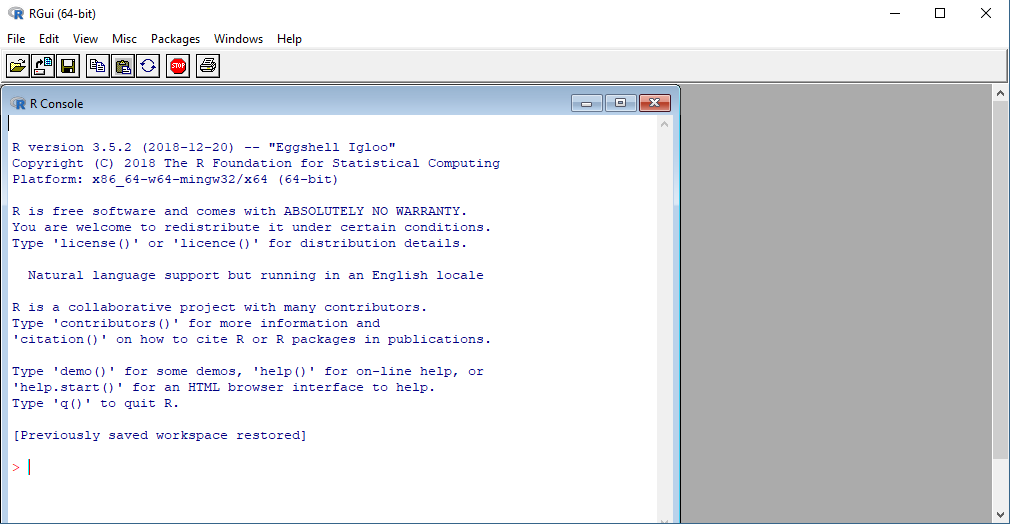
\includegraphics[width=0.8\linewidth]{jendela_r} 

}

\caption{Jendela R.}\label{fig:jendela-R}
\end{figure}

\begin{figure}

{\centering 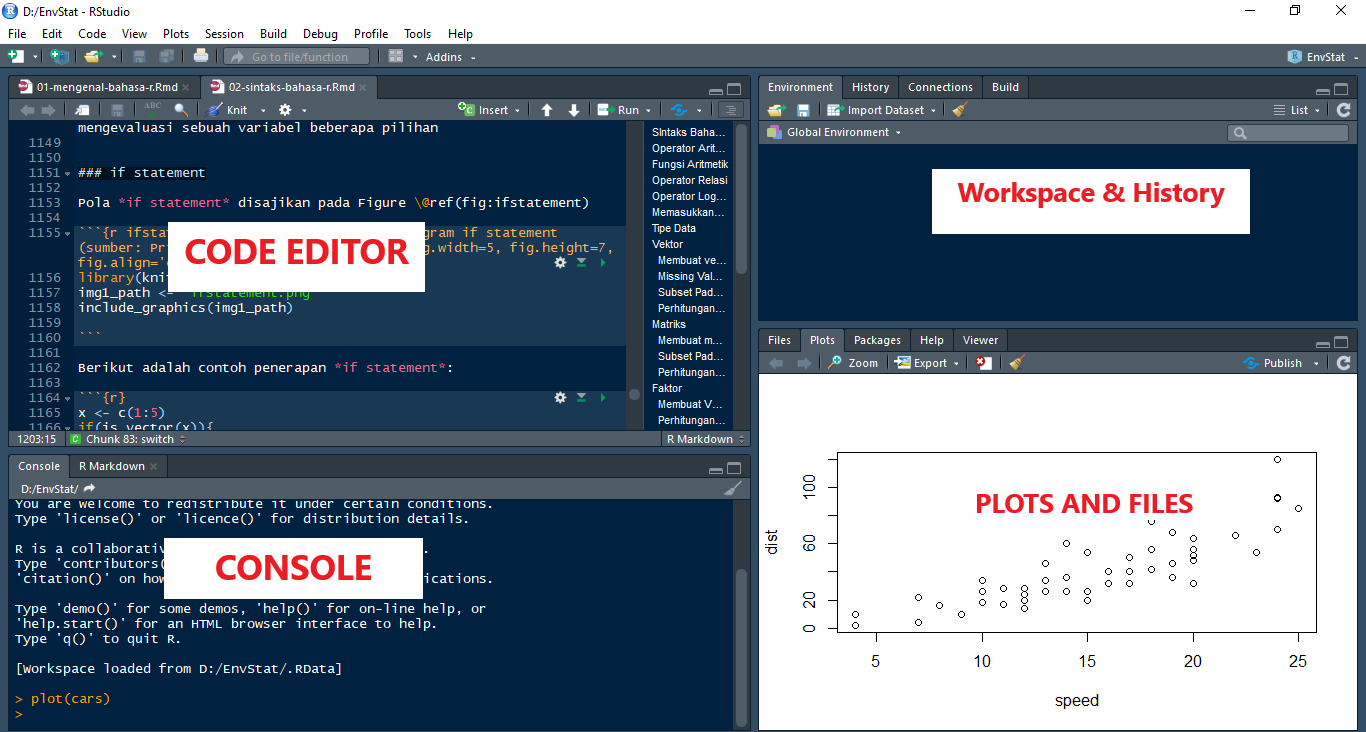
\includegraphics[width=0.8\linewidth]{jendela_rstudio} 

}

\caption{Jendela RStudio.}\label{fig:jendela-RStudio}
\end{figure}

\begin{quote}
\textbf{Note: } Sebaiknya install \texttt{R} terlebih dahulu sebelum
\texttt{RStudio}
\end{quote}

\section{Working Directory}\label{working-directory}

Setiap pengguna akan bekerja pada tempat khusus yang disebut sebagai
\emph{working directory}. \emph{working directory} merupakan sebuah
folder dimana \texttt{R} akan membaca dan menyimpan file kerja kita.
Pada pengguna \texttt{windows}, \emph{working directory} secara default
pada saat pertama kali menginstall \texttt{R} terletak pada folder
\texttt{c:\textbackslash{}\textbackslash{}Document}.

\subsection{Mengubah Lokasi Working
Directory}\label{mengubah-lokasi-working-directory}

Kita dapat mengubah lokasi \emph{working directory} berdasarkan lokasi
yang kita inginkan, misalnya letak data yang akan kita olah tidak ada
pada folder default atau kita ingin pekerjaan kita terkait \texttt{R}
dapat berlangsung pada satu folder khusus.

Berikut adalah cara mengubah \emph{working directory} pada \texttt{R}.

\begin{enumerate}
\def\labelenumi{\arabic{enumi}.}
\tightlist
\item
  Buatlah folder pada drive (kita bisa membuat folder pada selain drive
  c) dan namai dengan nama yang kalian inginkan. Pada tutorial ini
  penulis menggunakan nama folder \texttt{R}.
\item
  Jika pengguna menggunakan \texttt{RStudio}, pada menu \texttt{RStudio}
  pilih \textbf{Session \textgreater{} Set Working Directory
  \textgreater{} Chooses Directory}. Proses tersebut ditampilkan pada
  Figure \ref{fig:working}
\item
  Pilih folder yang telah dibuat pada step 1 sebagai *working directory.
\end{enumerate}

\begin{quote}
\textbf{Note: } Data atau file yang hendak dibaca selama proses kerja
pada \texttt{R} harus selalu diletakkan pada working directory. Jika
tidak maka data atau file tidak akan terbaca.
\end{quote}

Untuk mengecek apakah proses perubahan telah terjadi, kita dapat
mengeceknya dengan menjalankan perintah berikut untuk melihat lokasi
\emph{working directory} kita yang baru.

\begin{Shaded}
\begin{Highlighting}[]
\KeywordTok{getwd}\NormalTok{()}
\end{Highlighting}
\end{Shaded}

\begin{figure}

{\centering 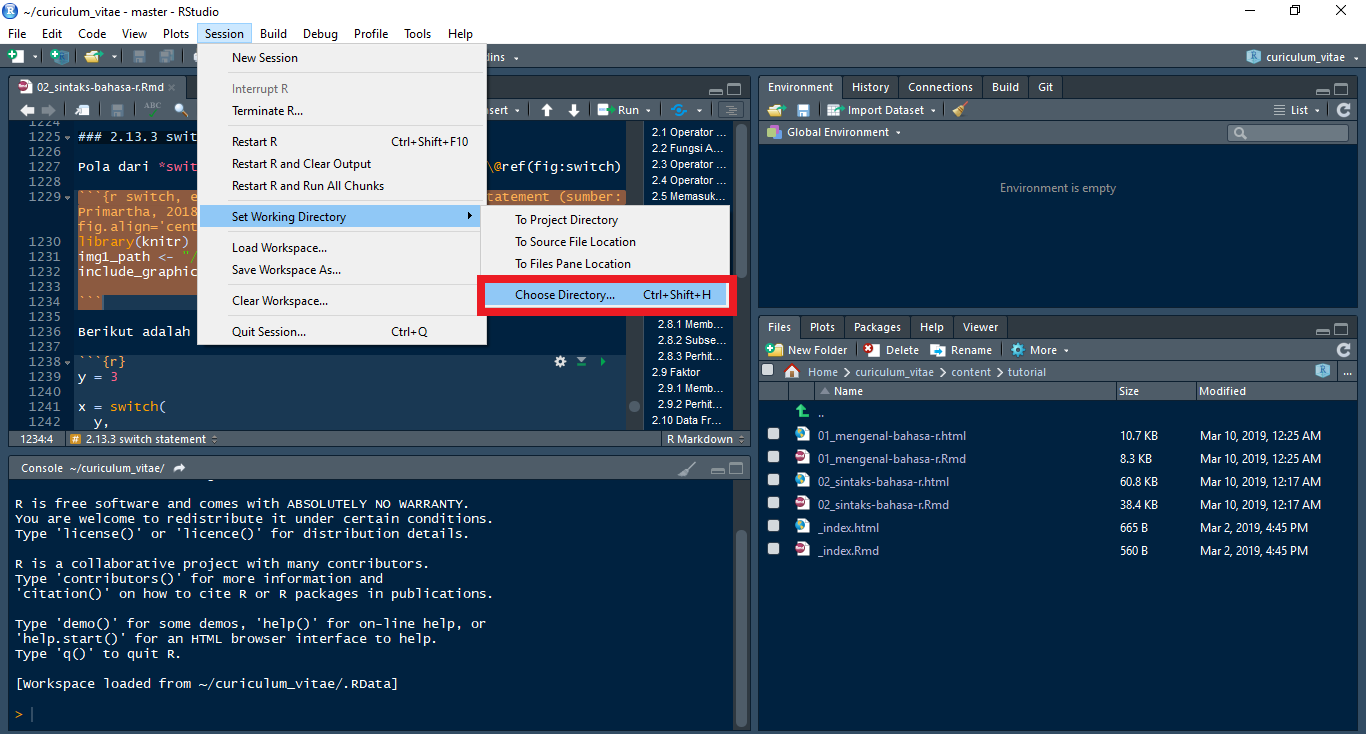
\includegraphics[width=0.8\linewidth]{working} 

}

\caption{Mengubah working directory.}\label{fig:working}
\end{figure}

Selain itu kita dapat mengubah \emph{working directory} menggunakan
perintah berikut:

\begin{Shaded}
\begin{Highlighting}[]
\CommentTok{# Ubah working directori pada folder R}
\KeywordTok{setwd}\NormalTok{(}\StringTok{"/Documents/R"}\NormalTok{)}
\end{Highlighting}
\end{Shaded}

\begin{quote}
\textbf{Note: } Pada proses pengisian lokasi folder pastikan pemisah
pada lokasi folder menggunakan tanda ``/'' bukan ``"
\end{quote}

\subsection{Mengubah Lokasi Working Directory
Default}\label{mengubah-lokasi-working-directory-default}

Pada proses yang telah penulis jelaskan sebelumnya. Proses perubahan
\emph{working directory} hanya berlaku pada saat pekerjaan tersebut
dilakukan. Setelah pekerjaan selesai dan kita menjalankan kembali
\texttt{R} maka \emph{working directory} akan kembali secara default
pada working directory lama.

Untuk membuat lokasi default \emph{working directory} pindah, kita dapat
melakukannya dengan memilih pada menu: \textbf{Tools \textgreater{}
Global options \textgreater{} pada ``General'' klik pada ``Browse'' dan
pilih lokasi working directory yang diinginkan}. Proses tersebut
ditampilkan pada Figure \ref{fig:default}

\begin{figure}

{\centering 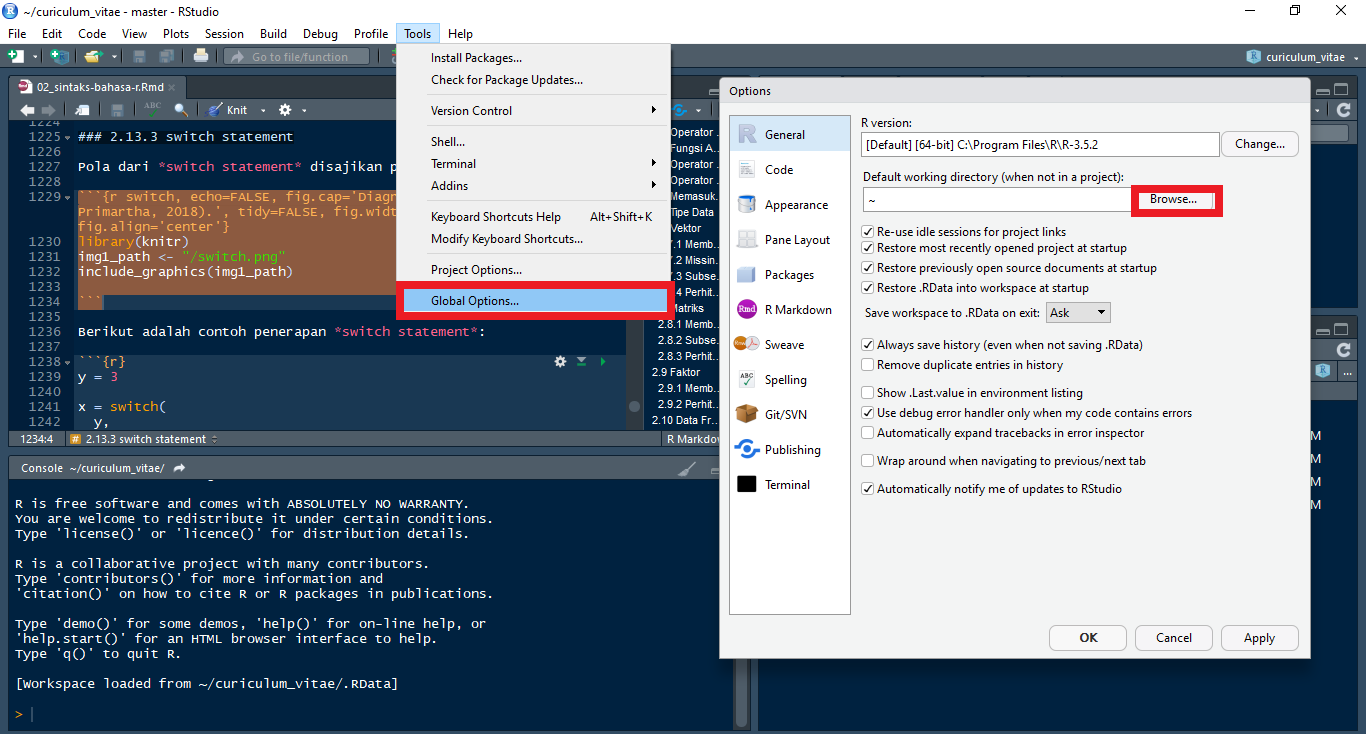
\includegraphics[width=0.8\linewidth]{default} 

}

\caption{Merubah working directory melalui Global options.}\label{fig:default}
\end{figure}

\section{Fasilitas Help}\label{fasilitas-help}

Agar dapat menggunakan \texttt{R} dengan secara lebih baik, pengetahuan
untuk mengakses fasilitas \emph{help} in cukup penting untuk
disampaikan. Adapun cara yang dapat digunakan adalah sebagai berikut.

\subsection{Mencari Help dari Suatu Perintah
Tertentu}\label{mencari-help-dari-suatu-perintah-tertentu}

Untuk memperoleh bantuan terkait suatu perintah tertentu kita dapat
menggunakan fungsi \texttt{help()}. Secara umum format yang digunakan
adalah sebagai berikut:

\begin{Shaded}
\begin{Highlighting}[]
\KeywordTok{help}\NormalTok{(nama_perintah)}
\end{Highlighting}
\end{Shaded}

atau dapat juga menggunakan tanda tanya (?) pada awal
\texttt{nama\_perintah} seperti berikut:

\begin{Shaded}
\begin{Highlighting}[]
\NormalTok{?nama_perintah}
\end{Highlighting}
\end{Shaded}

Misalkan kita kebingungan terkait bagaimana cara menuliskan perintah
untuk menghitung rata-rata suatu vektor. Kita dapat mengetikkan perintah
berikut untuk mengakses fasilitas \emph{help}.

\begin{Shaded}
\begin{Highlighting}[]
\KeywordTok{help}\NormalTok{(mean)}

\CommentTok{#atau}
\NormalTok{?mean}
\end{Highlighting}
\end{Shaded}

Perintah tersebut akan memunculkan hasil berupa dokumentasi yang
ditampilkan pada Figure \ref{fig:meandoc}.

\begin{figure}

{\centering 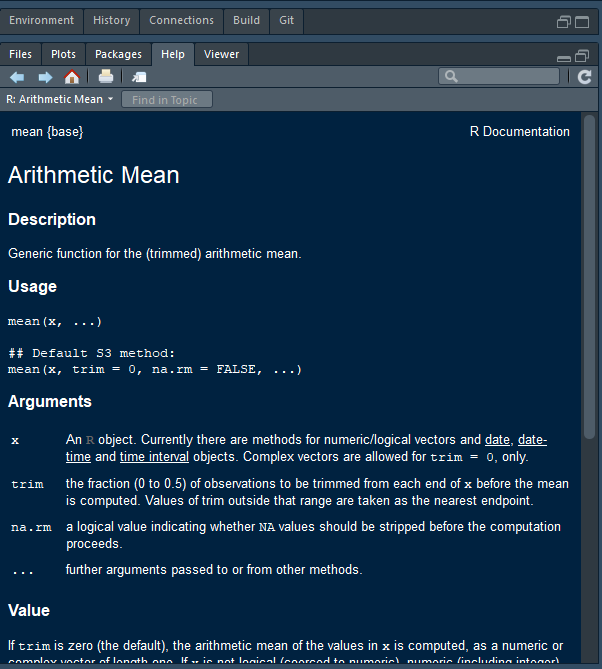
\includegraphics[width=0.5\linewidth]{meandoc} 

}

\caption{Jendela help dokumentasi fungsi mean().}\label{fig:meandoc}
\end{figure}

Keterangan pada jendela pada Figure \ref{fig:meandoc} adalah sebagia
berikut:

\begin{enumerate}
\def\labelenumi{\arabic{enumi}.}
\tightlist
\item
  Pada bagian jendela kiri atas jendela \emph{help}, diberikan
  keterangan nama dari perintah yang sedang ditampilkan.
\item
  Selanjutnya, pada bagian atas dokumen, ditampilkan infomasi terkait
  nama perintah, dan nama \emph{library} yang memuat perintah tersebut.
  Pada gambar diatas informasi terkait perintah dan nama \emph{library}
  ditunjukkan pada teks \texttt{mean\ \{base\}} yang menunjukkan
  perintah \texttt{mean()} pada paket (\emph{library}) \emph{base}
  (paket bawaan \texttt{R}).
\item
  Setiap jendela \emph{help} dari suatu perintah tertentu selanjutnya
  akan memuat bagian-bagian berikut:
\end{enumerate}

\begin{itemize}
\tightlist
\item
  \emph{Title}
\item
  \emph{Description} : deskripsi singkat tentang perintah.
\item
  \emph{Usage} : menampilkan sintaks perintah untuk penggunaan perintah
  tersebut.
\item
  \emph{Arguments} : keterangan mengenai \emph{argument/input}yang
  diperlukan pada perintah tersebut.
\item
  \emph{Details} : keterangan lebih lengkap lengkap tentang perintah
  tersebut.
\item
  \emph{Value} : keterangan tentang \emph{output} suatu perintah dapat
  diperoleh pada bagian ini.
\item
  \emph{Author(s)} : memberikan keterangan tentang \emph{Author} dari
  perintah tersebut.
\item
  \emph{References} : seringkali referensi yang dapat digunakan untuk
  memperoleh keterangan lebih lanjut terhadap suatu perintah ditampilkan
  pada bagian ini.
\item
  \emph{See also}: bagian ini berisikan daftar perintah/fungsi yang
  berhubungan erat dengan perintah tersebut.
\item
  \emph{Example} : berisikan contoh-contoh penggunaan perintah tersebut.
\end{itemize}

Kita juga dapat melihat contoh penggunaan dari perintah tersebut. Untuk
melakukannya kita dapat menggunakan fungsi \texttt{example()}. Fungsi
tersebut akan menampilkan contoh kode penerapan dari fungsi yang kita
inginkan. Secara sederhana fungsi tersebut dapat dituliskan sebagai
berikut:

\begin{Shaded}
\begin{Highlighting}[]
\KeywordTok{example}\NormalTok{(nama_perintah)}
\end{Highlighting}
\end{Shaded}

Untuk mengetahui contoh kode fungsi \texttt{mean()}, ketikkan sintaks
berikut:

\begin{Shaded}
\begin{Highlighting}[]
\KeywordTok{example}\NormalTok{(mean)}
\end{Highlighting}
\end{Shaded}

\begin{verbatim}
## 
## mean> x <- c(0:10, 50)
## 
## mean> xm <- mean(x)
## 
## mean> c(xm, mean(x, trim = 0.10))
## [1] 8.75 5.50
\end{verbatim}

kita juga dapat mencoba kode yang dihasilkan pada console \texttt{R}.
Berikut adalah contoh penerapannya:

\begin{Shaded}
\begin{Highlighting}[]
\CommentTok{# Menghitung rata-rata bilangan 1 sampai 10 dan 50}
\CommentTok{# membuat vektor}
\NormalTok{x <-}\StringTok{ }\KeywordTok{c}\NormalTok{(}\DecValTok{0}\OperatorTok{:}\DecValTok{10}\NormalTok{, }\DecValTok{50}\NormalTok{)}

\CommentTok{# Print}
\NormalTok{x}
\end{Highlighting}
\end{Shaded}

\begin{verbatim}
##  [1]  0  1  2  3  4  5  6  7  8  9 10 50
\end{verbatim}

\begin{Shaded}
\begin{Highlighting}[]
\CommentTok{# mean}
\KeywordTok{mean}\NormalTok{(x)}
\end{Highlighting}
\end{Shaded}

\begin{verbatim}
## [1] 8.75
\end{verbatim}

Pembaca dapat mencoba melakukanya sendiri dengan mengganti nilai yang
telah ada serta mencoba contoh kode yang lain.

\subsection{General Help}\label{general-help}

Kita juga dapat membaca beberapa dokumen manual yang ada pada
\texttt{R}. Untuk melakukannya jalankan perintah berikut:

\begin{Shaded}
\begin{Highlighting}[]
\KeywordTok{help.start}\NormalTok{()}
\end{Highlighting}
\end{Shaded}

Output yang dihasilkan berupa link pada sejumlah dokumen yang dapat kita
klik. Tampilan halaman yang dihasilkan disajikan pada Figure
\ref{fig:generalhelp}.

\begin{figure}

{\centering 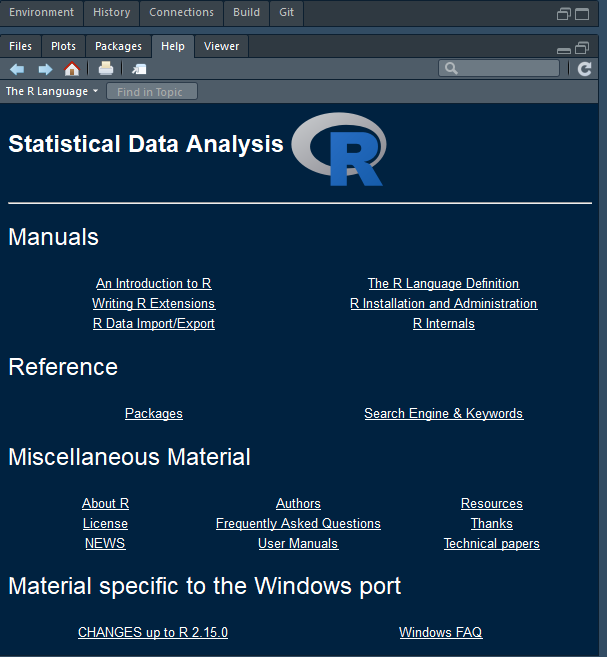
\includegraphics[width=0.5\linewidth]{generalhelp} 

}

\caption{Jendela general help dokumentasi fungsi mean().}\label{fig:generalhelp}
\end{figure}

\subsection{Fasilitas Help Lainnya}\label{fasilitas-help-lainnya}

Selain yang telah penulis sebutkan sebelumnya. Kita juga dapat
memanfaatkan fasilitas \emph{help} lainnya melalui fungsi
\texttt{apropos()} dan \texttt{help.search()}.

\texttt{apropos\ ()}: mengembalikan daftar objek, berisi pola yang
pembaca cari, dengan pencocokan sebagian. Ini berguna ketika pembaca
tidak ingat persis nama fungsi yang akan digunakan. Berikut adalah
contoh ketika penulis ingin mengetahui fungsi yang digunakan untuk
menghitung median.

\begin{Shaded}
\begin{Highlighting}[]
\KeywordTok{apropos}\NormalTok{(}\StringTok{"med"}\NormalTok{)}
\end{Highlighting}
\end{Shaded}

\begin{verbatim}
##  [1] "elNamed"         "elNamed<-"       "interp.median"  
##  [4] "median"          "median.default"  "median_hilow"   
##  [7] "mediate"         "mediate.diagram" "medpolish"      
## [10] "runmed"
\end{verbatim}

\emph{List} yang dihasilkan berupa fungsi-fungsi yang memiliki elemen
kata ``med''. Berdasarkan pencaria tersebut penulis dapat mencoba
menggunakan fungsi ``median'' untuk menghitung median.

\texttt{help.search\ ()} (sebagai alternatif ??): mencari dokumentasi
yang cocok dengan karakter yang diberikan dengan cara yang berbeda. Ini
mengembalikan daftar fungsi yang mengandung istilah yang pembaca cari
dengan deskripsi singkat dari fungsi.

Berikut adalah contoh penerapan dari fungsi tersebut:

\begin{Shaded}
\begin{Highlighting}[]
\KeywordTok{help.search}\NormalTok{(}\StringTok{"mean"}\NormalTok{)}

\CommentTok{# atau}
\NormalTok{??mean}
\end{Highlighting}
\end{Shaded}

\emph{Output} yang dihasilkan akan tampak seperti pada Figure
\ref{fig:helpsearch}.

\begin{figure}

{\centering 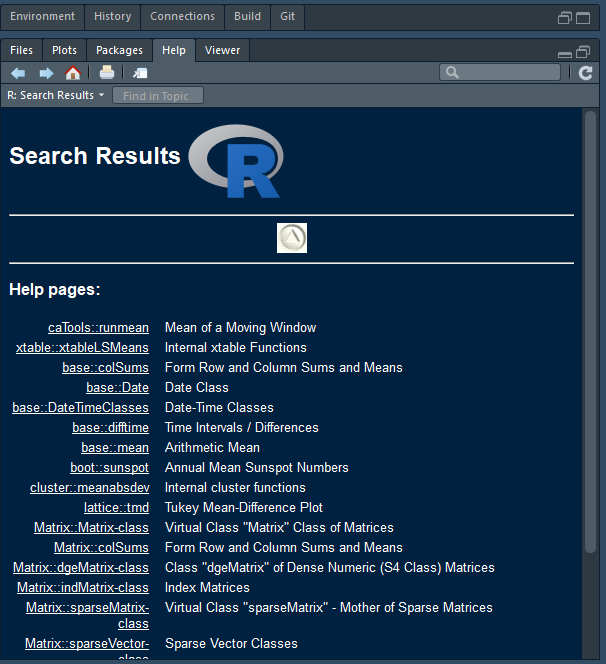
\includegraphics[width=0.5\linewidth]{helpsearch} 

}

\caption{Jendela help search dokumentasi fungsi mean().}\label{fig:helpsearch}
\end{figure}

\section{Referensi}\label{referensi}

\begin{enumerate}
\def\labelenumi{\arabic{enumi}.}
\tightlist
\item
  Primartha, R. 2018. \textbf{Belajar Machine Learning Teori dan
  Praktik}. Penerbit Informatika : Bandung
\item
  Rosadi,D. 2016. \textbf{Analisis Statistika dengan R}. Gadjah Mada
  University Press: Yogyakarta
\item
  STHDA. Running RStudio and Setting Up Your Working Directory - Easy R
  Programming
  .\url{http://www.sthda.com/english/wiki/running-rstudio-and-setting-up-your-working-directory-easy-r-programming\#set-your-working-directory}
\item
  STDHA. \textbf{Getting Help With Functions In R Programming}.
  \url{http://www.sthda.com/english/wiki/getting-help-with-functions-in-r-programming}
  .
\item
  Venables, W.N. Smith D.M. and R Core Team. 2018. \textbf{An
  Introduction to R}. R Manuals.
\end{enumerate}

\chapter{Sintaks Bahasa R}\label{sintaks-bahasa-r}

Pada \emph{chapter} ini penulis hendak mengajak pembaca lebih familiar
dengan sintaks atau perintah yang ada pada \texttt{R}. Pembaca akan
mempelajari penggunaan operator dalam melakukan operasi pengolahan data
pada \texttt{R}, jenis data yang ada pada \texttt{R}, sampai dengan
bagaimana kita melakukan proses \emph{decision making} menggunakan
\texttt{R}.

\section{Operator Aritmatika}\label{operator-aritmatika}

Proses perhitungan akan ditangani oleh fungsi khusus. \texttt{R} akan
memahami urutannya secara benar. Kecuali kita secara eksplisit
menetapkan yang lain. Sebagai contoh jalankan sintaks berikut:

\begin{Shaded}
\begin{Highlighting}[]
\DecValTok{2}\OperatorTok{+}\DecValTok{4}\OperatorTok{*}\DecValTok{2}
\end{Highlighting}
\end{Shaded}

\begin{verbatim}
## [1] 10
\end{verbatim}

Bandingkan dengan sintaks berikut:

\begin{Shaded}
\begin{Highlighting}[]
\NormalTok{(}\DecValTok{2}\OperatorTok{+}\DecValTok{4}\NormalTok{)}\OperatorTok{*}\DecValTok{2}
\end{Highlighting}
\end{Shaded}

\begin{verbatim}
## [1] 12
\end{verbatim}

\begin{quote}
\texttt{R} dapat digunakan sebagai kalkulator
\end{quote}

Berdasarkan kedua hasil tersebut dapat disimpulkan bahwa ketika kita
tidak menetapkan urutan perhitungan menggunakan tanda kurung, \texttt{R}
akan secara otomatis akan menghitung terlebih dahulu perkalian atau
pembangian.

Operator aritmatika yang disediakan \texttt{R} adalah sebagai berikut:

\textbf{Table 1} Operator Aritmatika \texttt{R}

\begin{longtable}[]{@{}ll@{}}
\toprule
\begin{minipage}[b]{0.15\columnwidth}\raggedright\strut
\textbf{Simbol}\strut
\end{minipage} & \begin{minipage}[b]{0.79\columnwidth}\raggedright\strut
\textbf{Keterangan}\strut
\end{minipage}\tabularnewline
\midrule
\endhead
\begin{minipage}[t]{0.15\columnwidth}\raggedright\strut
+\strut
\end{minipage} & \begin{minipage}[t]{0.79\columnwidth}\raggedright\strut
\emph{Addition}, untuk operasi penjumlahan\strut
\end{minipage}\tabularnewline
\begin{minipage}[t]{0.15\columnwidth}\raggedright\strut
-\strut
\end{minipage} & \begin{minipage}[t]{0.79\columnwidth}\raggedright\strut
\emph{Substraction}, untuk operasi pengurangan\strut
\end{minipage}\tabularnewline
\begin{minipage}[t]{0.15\columnwidth}\raggedright\strut
*\strut
\end{minipage} & \begin{minipage}[t]{0.79\columnwidth}\raggedright\strut
\emph{Multiplication}, untuk operasi pembagian\strut
\end{minipage}\tabularnewline
\begin{minipage}[t]{0.15\columnwidth}\raggedright\strut
/\strut
\end{minipage} & \begin{minipage}[t]{0.79\columnwidth}\raggedright\strut
\emph{Division}, untuk operasi pembagian\strut
\end{minipage}\tabularnewline
\begin{minipage}[t]{0.15\columnwidth}\raggedright\strut
\^{}\strut
\end{minipage} & \begin{minipage}[t]{0.79\columnwidth}\raggedright\strut
\emph{Eksponentiation}, untuk operasi pemangkatan\strut
\end{minipage}\tabularnewline
\begin{minipage}[t]{0.15\columnwidth}\raggedright\strut
\%\%\strut
\end{minipage} & \begin{minipage}[t]{0.79\columnwidth}\raggedright\strut
\emph{Modulus}, Untuk mencari sisa pembagian\strut
\end{minipage}\tabularnewline
\begin{minipage}[t]{0.15\columnwidth}\raggedright\strut
\%/\%\strut
\end{minipage} & \begin{minipage}[t]{0.79\columnwidth}\raggedright\strut
\emph{Integer}, Untuk mencari bilangan bulat hasil pembagian saja dan
tanpa sisa pembagian\strut
\end{minipage}\tabularnewline
\bottomrule
\end{longtable}

Untuk lebih memahaminya berikut contoh sintaks penerapan operator
tersebut.

\begin{Shaded}
\begin{Highlighting}[]
\CommentTok{# Addition}
\DecValTok{5}\OperatorTok{+}\DecValTok{3}
\end{Highlighting}
\end{Shaded}

\begin{verbatim}
## [1] 8
\end{verbatim}

\begin{Shaded}
\begin{Highlighting}[]
\CommentTok{# Substraction}
\DecValTok{5}\OperatorTok{-}\DecValTok{3}
\end{Highlighting}
\end{Shaded}

\begin{verbatim}
## [1] 2
\end{verbatim}

\begin{Shaded}
\begin{Highlighting}[]
\CommentTok{# Multiplication}
\DecValTok{5}\OperatorTok{*}\DecValTok{3}
\end{Highlighting}
\end{Shaded}

\begin{verbatim}
## [1] 15
\end{verbatim}

\begin{Shaded}
\begin{Highlighting}[]
\CommentTok{# Division}
\DecValTok{5}\OperatorTok{/}\DecValTok{3}
\end{Highlighting}
\end{Shaded}

\begin{verbatim}
## [1] 1.666667
\end{verbatim}

\begin{Shaded}
\begin{Highlighting}[]
\CommentTok{# Eksponetiation}
\DecValTok{5}\OperatorTok{^}\DecValTok{3}
\end{Highlighting}
\end{Shaded}

\begin{verbatim}
## [1] 125
\end{verbatim}

\begin{Shaded}
\begin{Highlighting}[]
\CommentTok{# Modulus}
\DecValTok{5}\OperatorTok\DecValTok{3}
\end{Highlighting}
\end{Shaded}

\begin{verbatim}
## [1] 2
\end{verbatim}

\begin{Shaded}
\begin{Highlighting}[]
\CommentTok{# Integer}
\DecValTok{5}\OperatorTok\DecValTok{3}
\end{Highlighting}
\end{Shaded}

\begin{verbatim}
## [1] 1
\end{verbatim}

\begin{quote}
\emph{Note: } Pada \texttt{R} tanda \texttt{\#} berfungsi menambahkan
keterangan untuk menjelaskan sebuah sintaks pada \texttt{R}.
\end{quote}

\section{Fungsi Aritmetik}\label{fungsi-aritmetik}

Selain fungsi operator aritmetik, pada \texttt{R} juga telah tersedia
fungsi aritmetik yang lain seperti logaritmik, ekponensial,
trigonometri, dll.

\begin{enumerate}
\def\labelenumi{\arabic{enumi}.}
\tightlist
\item
  Logaritma dan eksponensial
\end{enumerate}

Untuk contoh fungsi logaritmik dan eksponensial jalankan sintaks
berikut:

\begin{Shaded}
\begin{Highlighting}[]
\KeywordTok{log2}\NormalTok{(}\DecValTok{8}\NormalTok{) }\CommentTok{# logaritma basis 2 untuk 8}
\end{Highlighting}
\end{Shaded}

\begin{verbatim}
## [1] 3
\end{verbatim}

\begin{Shaded}
\begin{Highlighting}[]
\KeywordTok{log10}\NormalTok{(}\DecValTok{8}\NormalTok{) }\CommentTok{# logaritma basis 10 untuk 8}
\end{Highlighting}
\end{Shaded}

\begin{verbatim}
## [1] 0.90309
\end{verbatim}

\begin{Shaded}
\begin{Highlighting}[]
\KeywordTok{exp}\NormalTok{(}\DecValTok{8}\NormalTok{) }\CommentTok{# eksponensial 8}
\end{Highlighting}
\end{Shaded}

\begin{verbatim}
## [1] 2980.958
\end{verbatim}

\begin{enumerate}
\def\labelenumi{\arabic{enumi}.}
\setcounter{enumi}{1}
\tightlist
\item
  Fungsi trigonometri
\end{enumerate}

fungsi trigonometri yang ditampilkan seperti sin,cos, tan, dll.

\begin{Shaded}
\begin{Highlighting}[]
\KeywordTok{cos}\NormalTok{(x) }\CommentTok{# cos x}
\KeywordTok{sin}\NormalTok{(x) }\CommentTok{# Sin x}
\KeywordTok{tan}\NormalTok{(x) }\CommentTok{# Tan x}
\KeywordTok{acos}\NormalTok{(x) }\CommentTok{# arc-cos x}
\KeywordTok{asin}\NormalTok{(x) }\CommentTok{# arc-sin x}
\KeywordTok{atan}\NormalTok{(x) }\CommentTok{#arc-tan x}
\end{Highlighting}
\end{Shaded}

\begin{quote}
\textbf{Note: } x dalam fungsi trigonometri memiliki satuan radian
\end{quote}

Berikut adalah salah satu contoh penggunaannya:

\begin{Shaded}
\begin{Highlighting}[]
\KeywordTok{cos}\NormalTok{(pi)}
\end{Highlighting}
\end{Shaded}

\begin{verbatim}
## [1] -1
\end{verbatim}

\begin{enumerate}
\def\labelenumi{\arabic{enumi}.}
\setcounter{enumi}{2}
\tightlist
\item
  Fungsi matematik lainnya
\end{enumerate}

Fungsi lainnya yang dapat digunakan adalah fungsi absolut, akar kuadrat,
dll. Berikut adalah contoh sintaks penggunaan fungsi absolut dan akar
kuadrat.

\begin{Shaded}
\begin{Highlighting}[]
\KeywordTok{abs}\NormalTok{(}\OperatorTok{-}\DecValTok{2}\NormalTok{) }\CommentTok{# nilai absolut -2}
\end{Highlighting}
\end{Shaded}

\begin{verbatim}
## [1] 2
\end{verbatim}

\begin{Shaded}
\begin{Highlighting}[]
\KeywordTok{sqrt}\NormalTok{(}\DecValTok{4}\NormalTok{) }\CommentTok{# akar kuadrat 4}
\end{Highlighting}
\end{Shaded}

\begin{verbatim}
## [1] 2
\end{verbatim}

\section{Operator Relasi}\label{operator-relasi}

Operator relasi digunakan untuk membandingkan satu objek dengan objek
lainnya. Operator yang disediakan \texttt{R} disajikan pada Table 2.

\textbf{Table 2} Operator Relasi \texttt{R}

\begin{longtable}[]{@{}ll@{}}
\toprule
\textbf{Simbol} & \textbf{Keterangan}\tabularnewline
\midrule
\endhead
``\textgreater{}'' & Lebih besar dari\tabularnewline
``\textless{}'' & Lebih Kecil dari\tabularnewline
``=='' & Sama dengan\tabularnewline
``\textgreater{}='' & Lebih besar sama dengan\tabularnewline
``\textless{}='' & Lebih kecil sama dengan\tabularnewline
``!='' & Tidak sama dengan\tabularnewline
\bottomrule
\end{longtable}

Berikut adalah penerapan operator pada tabel tersebut:

\begin{Shaded}
\begin{Highlighting}[]
\NormalTok{x <-}\StringTok{ }\DecValTok{34}
\NormalTok{y <-}\StringTok{ }\DecValTok{35}

\CommentTok{# Operator >}
\NormalTok{x }\OperatorTok{>}\StringTok{ }\NormalTok{y}
\end{Highlighting}
\end{Shaded}

\begin{verbatim}
## [1] FALSE
\end{verbatim}

\begin{Shaded}
\begin{Highlighting}[]
\CommentTok{# Operator <}
\NormalTok{x }\OperatorTok{<}\StringTok{ }\NormalTok{y}
\end{Highlighting}
\end{Shaded}

\begin{verbatim}
## [1] TRUE
\end{verbatim}

\begin{Shaded}
\begin{Highlighting}[]
\CommentTok{# operator ==}
\NormalTok{x }\OperatorTok{==}\StringTok{ }\NormalTok{y}
\end{Highlighting}
\end{Shaded}

\begin{verbatim}
## [1] FALSE
\end{verbatim}

\begin{Shaded}
\begin{Highlighting}[]
\CommentTok{# Operator >=}
\NormalTok{x }\OperatorTok{>=}\StringTok{ }\NormalTok{y}
\end{Highlighting}
\end{Shaded}

\begin{verbatim}
## [1] FALSE
\end{verbatim}

\begin{Shaded}
\begin{Highlighting}[]
\CommentTok{# Operator <=}
\NormalTok{x }\OperatorTok{<=}\StringTok{ }\NormalTok{y}
\end{Highlighting}
\end{Shaded}

\begin{verbatim}
## [1] TRUE
\end{verbatim}

\begin{Shaded}
\begin{Highlighting}[]
\CommentTok{# Operator !=}
\NormalTok{x }\OperatorTok{!=}\StringTok{ }\NormalTok{y}
\end{Highlighting}
\end{Shaded}

\begin{verbatim}
## [1] TRUE
\end{verbatim}

\section{Operator Logika}\label{operator-logika}

Operator logika hanya berlaku pada vektor dengan tipe logical, numeric,
atau complex. Semua angka bernilai 1 akan dianggap bernilai logika
\texttt{TRUE}. Operator logika yang disediakan \texttt{R} dapat dilihat
pada Table 3.

\textbf{Table 3} Operator logika \texttt{R}

\begin{longtable}[]{@{}ll@{}}
\toprule
\textbf{Simbol} & \textbf{Keterangan}\tabularnewline
\midrule
\endhead
\&\& & Operator logika AND\tabularnewline
&\tabularnewline
! & Opeartor logika NOT\tabularnewline
\& & Operator logika AND element wise\tabularnewline
& Operator logika OR element wise\tabularnewline
\bottomrule
\end{longtable}

Penerapannya terdapat pada sintaks berikut:

\begin{Shaded}
\begin{Highlighting}[]
\NormalTok{v <-}\StringTok{ }\KeywordTok{c}\NormalTok{(}\OtherTok{TRUE}\NormalTok{,}\OtherTok{TRUE}\NormalTok{, }\OtherTok{FALSE}\NormalTok{)}
\NormalTok{t <-}\StringTok{ }\KeywordTok{c}\NormalTok{(}\OtherTok{FALSE}\NormalTok{,}\OtherTok{FALSE}\NormalTok{,}\OtherTok{FALSE}\NormalTok{)}

\CommentTok{# Operator &&}
\KeywordTok{print}\NormalTok{(v}\OperatorTok{&&}\NormalTok{t)}
\end{Highlighting}
\end{Shaded}

\begin{verbatim}
## [1] FALSE
\end{verbatim}

\begin{Shaded}
\begin{Highlighting}[]
\CommentTok{# Operator ||}
\KeywordTok{print}\NormalTok{(v}\OperatorTok{||}\NormalTok{t)}
\end{Highlighting}
\end{Shaded}

\begin{verbatim}
## [1] TRUE
\end{verbatim}

\begin{Shaded}
\begin{Highlighting}[]
\CommentTok{# Operator !}
\KeywordTok{print}\NormalTok{(}\OperatorTok{!}\NormalTok{v)}
\end{Highlighting}
\end{Shaded}

\begin{verbatim}
## [1] FALSE FALSE  TRUE
\end{verbatim}

\begin{Shaded}
\begin{Highlighting}[]
\CommentTok{# operator &}
\KeywordTok{print}\NormalTok{(v}\OperatorTok{&}\NormalTok{t)}
\end{Highlighting}
\end{Shaded}

\begin{verbatim}
## [1] FALSE FALSE FALSE
\end{verbatim}

\begin{Shaded}
\begin{Highlighting}[]
\CommentTok{# Operator |}
\KeywordTok{print}\NormalTok{(v}\OperatorTok{|}\NormalTok{t)}
\end{Highlighting}
\end{Shaded}

\begin{verbatim}
## [1]  TRUE  TRUE FALSE
\end{verbatim}

\begin{quote}
\textbf{Note: }

operator \& dan \textbar{} akan mengecek logika tiap elemen pada vektor
secara berpesangan (sesuai urutan dari kiri ke kanan).

Operator \%\% dan \textbar{}\textbar{} hanya mengecek dari kiri ke kanan
pada observasi pertama. Misal saat menggunakan \&\& jika observasi
pertama TRUE maka observasi pertama pada vektor lainnya akan dicek,
namun jika observasi pertama FALSE maka proses akan segera dihentikan
dan menghasilkan FALSE.
\end{quote}

\section{Memasukkan Nilai Kedalam
Variabel}\label{memasukkan-nilai-kedalam-variabel}

Variabel pada \texttt{R} dapat digunakan untuk menyimpan nilai. Sebagai
contoh jalankan sintaks berikut:

\begin{Shaded}
\begin{Highlighting}[]
\CommentTok{# Harga sebuah lemon adalah 500 rupiah}
\NormalTok{lemon <-}\StringTok{ }\DecValTok{500}

\CommentTok{# Atau}
\DecValTok{500}\NormalTok{ ->}\StringTok{ }\NormalTok{lemon}

\CommentTok{# dapat juga menggunakan tanda "="}
\NormalTok{lemon =}\StringTok{ }\DecValTok{500}
\end{Highlighting}
\end{Shaded}

\begin{quote}
\textbf{Note: }

\begin{enumerate}
\def\labelenumi{\arabic{enumi}.}
\item
  \texttt{R} memungkinkan penggunaan \textless{}-,-\textgreater{}, atau
  = sebagai perintah pengisi nilai variabel
\item
  \texttt{R} bersifat \emph{case-sensitive}. Maksudnya adalah variabel
  Lemon tidak sama dengan lemon (Besar kecil huruf berpengaruh)
\end{enumerate}
\end{quote}

Untuk mengetahui nilai dari objek \texttt{lemon} kita dapat menggunakan
fungsi \texttt{print()} atau mengetikkan nama objeknya secara langsung.

\begin{Shaded}
\begin{Highlighting}[]
\CommentTok{# Menggunakan fungsi print()}
\KeywordTok{print}\NormalTok{(lemon)}
\end{Highlighting}
\end{Shaded}

\begin{verbatim}
## [1] 500
\end{verbatim}

\begin{Shaded}
\begin{Highlighting}[]
\CommentTok{# Atau}
\NormalTok{lemon}
\end{Highlighting}
\end{Shaded}

\begin{verbatim}
## [1] 500
\end{verbatim}

\texttt{R} akan menyimpan variabel \texttt{lemon} sebagai objek pada
memori. Sehingga kita dapat melakukan operasi terhadap objek tersebut
seperti mengalikannya atau menjumlahkannya dengan bilangan lain. Sebagai
contoh jalankan sintaks berikut:

\begin{Shaded}
\begin{Highlighting}[]
\CommentTok{# Operasi perkalian terhadap objek lemon}
\DecValTok{5}\OperatorTok{*}\NormalTok{lemon}
\end{Highlighting}
\end{Shaded}

\begin{verbatim}
## [1] 2500
\end{verbatim}

Kita dapat juga mengubah nilai dari objek \texttt{lemon} dengan cara
menginput nilai baru terhadap objek yang sama. \texttt{R} secara
otomatis akan menggatikan nilai sebelumnya. Untuk lebih memahaminya
jalankan sintaks berikut:

\begin{Shaded}
\begin{Highlighting}[]
\NormalTok{lemon <-}\StringTok{ }\DecValTok{1000}

\CommentTok{# Print lemon}
\KeywordTok{print}\NormalTok{(lemon)}
\end{Highlighting}
\end{Shaded}

\begin{verbatim}
## [1] 1000
\end{verbatim}

Untuk lebih memahaminya berikut adalah sintaks untuk menghitung volume
suatu objek.

\begin{Shaded}
\begin{Highlighting}[]
\CommentTok{# Dimensi objek}
\NormalTok{panjang <-}\StringTok{ }\DecValTok{10}
\NormalTok{lebar <-}\StringTok{ }\DecValTok{5}
\NormalTok{tinggi <-}\StringTok{ }\DecValTok{5}

\CommentTok{# Menghitung volume}
\NormalTok{volume <-}\StringTok{ }\NormalTok{panjang}\OperatorTok{*}\NormalTok{lebar}\OperatorTok{*}\NormalTok{tinggi}

\CommentTok{# Print objek volume}
\KeywordTok{print}\NormalTok{(volume)}
\end{Highlighting}
\end{Shaded}

\begin{verbatim}
## [1] 250
\end{verbatim}

Untuk mengetahui objek apa saja yang telah kita buat sepanjang artikel
ini kita dapang menggunakan fungsi \texttt{ls()}.

\begin{Shaded}
\begin{Highlighting}[]
\KeywordTok{ls}\NormalTok{()}
\end{Highlighting}
\end{Shaded}

\begin{verbatim}
##  [1] "A"         "B"         "img1_path" "lebar"     "lemon"    
##  [6] "panjang"   "t"         "tinggi"    "v"         "volume"   
## [11] "x"         "xm"        "y"
\end{verbatim}

\begin{quote}
Kumpulan objek yang telah tersimpan dalam memori disebut sebagai
\textbf{workspace}
\end{quote}

Untuk menghapus objek pada memori kita dapat menggunakan fungsi
\texttt{rm()}. Pada sintaks berikut penulis hendak menghapus objek
\texttt{lemon} dan \texttt{volume}.

\begin{Shaded}
\begin{Highlighting}[]
\CommentTok{# Menghapus objek lemon dan volume}
\KeywordTok{rm}\NormalTok{(lemon, volume)}

\CommentTok{# Tampilkan kembali objek yang tersisa}
\KeywordTok{ls}\NormalTok{()}
\end{Highlighting}
\end{Shaded}

\begin{verbatim}
##  [1] "A"         "B"         "img1_path" "lebar"     "panjang"  
##  [6] "t"         "tinggi"    "v"         "x"         "xm"       
## [11] "y"
\end{verbatim}

\begin{quote}
\textbf{Note: } Setiap variabel atau objek yang dibuat akan menempati
sejumlah memori pada komputer sehingga jika kita bekerja dengan jumlah
data yang banyak pastikan kita menghapus seluruh objek pada memori
sebelum memulai kerja.
\end{quote}

\section{Tipe Data}\label{tipe-data}

Data pada \texttt{R} dapat dikelompokan berdasarkan beberapa tipe. Tipe
data pada \texttt{R} disajikan pada Table 4.

\textbf{Table 4} Tipe Data \texttt{R}

\begin{longtable}[]{@{}lll@{}}
\toprule
\textbf{Tipe Data} & \textbf{Contoh} &
\textbf{Keterangan}\tabularnewline
\midrule
\endhead
Logical & TRUE, FALSE & Nilai Boolean\tabularnewline
Numeric & 12.3, 5, 999 & Segala jenis angka\tabularnewline
Integer & 23L, 97L, 3L & Bilangan integer (bilangan
bulat)\tabularnewline
Complex & 2i, 3i, 9i & Bilangan kompleks\tabularnewline
Character & `a', ``b'', ``123'' & Karakter dan string\tabularnewline
Raw & Identik dengan ``hello'' & Segala jenis data yang disimpan sebagai
raw bytes\tabularnewline
\bottomrule
\end{longtable}

Sintaks berikut adalah contoh dari tipe data pada \texttt{R}. Untuk
mengetahui tipa data suatu objek kita dapat menggunakan perintah
\texttt{class()}

\begin{Shaded}
\begin{Highlighting}[]
\CommentTok{# Logical}
\NormalTok{apel <-}\StringTok{ }\OtherTok{TRUE}
\KeywordTok{class}\NormalTok{(apel)}
\end{Highlighting}
\end{Shaded}

\begin{verbatim}
## [1] "logical"
\end{verbatim}

\begin{Shaded}
\begin{Highlighting}[]
\CommentTok{# Numeric}
\NormalTok{x <-}\StringTok{ }\FloatTok{2.3}
\KeywordTok{class}\NormalTok{(x)}
\end{Highlighting}
\end{Shaded}

\begin{verbatim}
## [1] "numeric"
\end{verbatim}

\begin{Shaded}
\begin{Highlighting}[]
\CommentTok{# Integer}
\NormalTok{y <-}\StringTok{ }\NormalTok{2L}
\KeywordTok{class}\NormalTok{(y)}
\end{Highlighting}
\end{Shaded}

\begin{verbatim}
## [1] "integer"
\end{verbatim}

\begin{Shaded}
\begin{Highlighting}[]
\CommentTok{# Compleks}
\NormalTok{z <-}\StringTok{ }\DecValTok{5}\OperatorTok{+}\NormalTok{2i}
\KeywordTok{class}\NormalTok{(z)}
\end{Highlighting}
\end{Shaded}

\begin{verbatim}
## [1] "complex"
\end{verbatim}

\begin{Shaded}
\begin{Highlighting}[]
\CommentTok{# string}
\NormalTok{w <-}\StringTok{ "saya"}
\KeywordTok{class}\NormalTok{(w)}
\end{Highlighting}
\end{Shaded}

\begin{verbatim}
## [1] "character"
\end{verbatim}

\begin{Shaded}
\begin{Highlighting}[]
\CommentTok{# Raw}
\NormalTok{xy <-}\StringTok{ }\KeywordTok{charToRaw}\NormalTok{(}\StringTok{"hello world"}\NormalTok{)}
\KeywordTok{class}\NormalTok{(xy)}
\end{Highlighting}
\end{Shaded}

\begin{verbatim}
## [1] "raw"
\end{verbatim}

Keenam jenis data tersebut disebut sebagai tipe data atomik. Hal ini
disebabkan karena hanya dapat menangani satu tipe data saja. Misalnya
hanya numeric atau hanya integer.

Selain menggunakan fungsi \texttt{class()}, kita dapat pula menggunakan
fungsi \texttt{is\_numeric()}, \texttt{is.character()},
\texttt{is.logical()}, dan sebagainya berdasarkan jenis data apa yang
ingin kita cek. Berbeda dengan fungsi \texttt{class()}, ouput yang
dihasilkan pada fungsi seperti \texttt{is\_numeric()} adalah nilai
Boolean sehingga fungsi ini hanya digunakan untuk mengecek apakah jenis
data pada objek sama seperti yang kita pikirkan. Sebagai contoh
disajikan pada sintaks berikut:

\begin{Shaded}
\begin{Highlighting}[]
\NormalTok{data <-}\StringTok{ }\DecValTok{25}

\CommentTok{# Cek apakah objek berisi data numerik}
\KeywordTok{is.numeric}\NormalTok{(data)}
\end{Highlighting}
\end{Shaded}

\begin{verbatim}
## [1] TRUE
\end{verbatim}

\begin{Shaded}
\begin{Highlighting}[]
\CommentTok{# Cek apakah objek adalah karakter}
\KeywordTok{is.character}\NormalTok{(data)}
\end{Highlighting}
\end{Shaded}

\begin{verbatim}
## [1] FALSE
\end{verbatim}

Kita juga dapat mengubah jenis data menjadi jenis lainnya seperti
integer menjadi numerik atau sebaliknya. Fungsi yang digunakan adalah
\texttt{as.numeric()} jika ingin mengubah suatu jenis data menjadi
numerik. Fungsi lainnya juga dapat digunakan sesuai dengan kita ingin
mengubah jenis data objek menjadi jenis data lainnya.

\begin{Shaded}
\begin{Highlighting}[]
\CommentTok{# Integer}
\NormalTok{apel <-}\StringTok{ }\NormalTok{2L}

\CommentTok{# Ubah menjadi numerik}
\KeywordTok{as.numeric}\NormalTok{(apel)}
\end{Highlighting}
\end{Shaded}

\begin{verbatim}
## [1] 2
\end{verbatim}

\begin{Shaded}
\begin{Highlighting}[]
\CommentTok{# Cek}
\KeywordTok{is.numeric}\NormalTok{(apel)}
\end{Highlighting}
\end{Shaded}

\begin{verbatim}
## [1] TRUE
\end{verbatim}

\begin{Shaded}
\begin{Highlighting}[]
\CommentTok{# Logical}
\NormalTok{nangka <-}\StringTok{ }\OtherTok{TRUE}

\CommentTok{# Ubah logical menjadi numeric}
\KeywordTok{as.numeric}\NormalTok{(nangka)}
\end{Highlighting}
\end{Shaded}

\begin{verbatim}
## [1] 1
\end{verbatim}

\begin{Shaded}
\begin{Highlighting}[]
\CommentTok{# Karakter}
\NormalTok{minum <-}\StringTok{ "minum"}

\CommentTok{# ubah karakter menjadi numerik}
\KeywordTok{as.numeric}\NormalTok{(minum)}
\end{Highlighting}
\end{Shaded}

\begin{verbatim}
## Warning: NAs introduced by coercion
\end{verbatim}

\begin{verbatim}
## [1] NA
\end{verbatim}

\begin{quote}
\textbf{Note: } Konversi karakter menjadi numerik akan menghasilkan
output NA (\emph{not available}). \texttt{R} tidak mengetahui bagaimana
cara merubah karakter menjadi bentuk numerik.
\end{quote}

Berdasarkan Tabel 2, vektor karakter dapat dibuat menggunakan tanda
kurung baik \emph{double quote} (``'') maupun \emph{single quote}
('').Jika pada teks yang kita tuliskan mengandung \emph{quote} maka kita
harus menghentikannya menggunakan tanda ( ~). Sbegai contoh kita ingin
menuliskan `\textbf{My friend's name is ``Adi''}, pada sintaks akan
dituliskan:

\begin{Shaded}
\begin{Highlighting}[]
\StringTok{'My friend\textbackslash{}`s name is "Adi"'}
\end{Highlighting}
\end{Shaded}

\begin{verbatim}
## [1] "My friend`s name is \"Adi\""
\end{verbatim}

\begin{Shaded}
\begin{Highlighting}[]
\CommentTok{# Atau}

\StringTok{"My friend's name }\CharTok{\textbackslash{}"}\StringTok{Adi}\CharTok{\textbackslash{}"}\StringTok{"}
\end{Highlighting}
\end{Shaded}

\begin{verbatim}
## [1] "My friend's name \"Adi\""
\end{verbatim}

\section{Vektor}\label{vektor}

Vektor merupakan kombinasi berbagai nilai (numerik, karakter, logical,
dan sebagainya berdasarkan jenis input data) pada objek yang sma. Pada
contoh kasus berikut, pembaca akan memiliki sesuai jenis data input
yaitu\textbf{vektor numerik}, \textbf{vector karakter}, \textbf{vektor
logical}, dll.

\subsection{Membuat vektor}\label{membuat-vektor}

Vektor dibuat dengan menggunakan fungsi \texttt{c()}(concatenate)
seperti yang disajikan pada sintaks berikut:

\begin{Shaded}
\begin{Highlighting}[]
\CommentTok{# membuat vektor numerik}
\NormalTok{x <-}\StringTok{ }\KeywordTok{c}\NormalTok{(}\DecValTok{3}\NormalTok{,}\FloatTok{3.5}\NormalTok{,}\DecValTok{4}\NormalTok{,}\DecValTok{7}\NormalTok{)}
\NormalTok{x }\CommentTok{# print vektor}
\end{Highlighting}
\end{Shaded}

\begin{verbatim}
## [1] 3.0 3.5 4.0 7.0
\end{verbatim}

\begin{Shaded}
\begin{Highlighting}[]
\CommentTok{# membuat vektor karakter}
\NormalTok{y <-}\StringTok{ }\KeywordTok{c}\NormalTok{(}\StringTok{"Apel"}\NormalTok{, }\StringTok{"Jeruk"}\NormalTok{, }\StringTok{"Rambutan"}\NormalTok{, }\StringTok{"Salak"}\NormalTok{)}
\NormalTok{y }\CommentTok{# print vektor}
\end{Highlighting}
\end{Shaded}

\begin{verbatim}
## [1] "Apel"     "Jeruk"    "Rambutan" "Salak"
\end{verbatim}

\begin{Shaded}
\begin{Highlighting}[]
\CommentTok{# membuat vektor logical}
\NormalTok{t <-}\StringTok{ }\KeywordTok{c}\NormalTok{(}\StringTok{"TRUE"}\NormalTok{, }\StringTok{"FALSE"}\NormalTok{, }\StringTok{"TRUE"}\NormalTok{)}
\NormalTok{t }\CommentTok{# print vektor}
\end{Highlighting}
\end{Shaded}

\begin{verbatim}
## [1] "TRUE"  "FALSE" "TRUE"
\end{verbatim}

selain menginput nilai pada vektor, kita juga dapat memberi nama nilai
setiap vektor menggunakan fungsi \texttt{names()}.

\begin{Shaded}
\begin{Highlighting}[]
\CommentTok{# Membuat vektor jumlah buah yang dibeli}
\NormalTok{Jumlah <-}\StringTok{ }\KeywordTok{c}\NormalTok{(}\DecValTok{5}\NormalTok{,}\DecValTok{5}\NormalTok{,}\DecValTok{6}\NormalTok{,}\DecValTok{7}\NormalTok{)}
\KeywordTok{names}\NormalTok{(Jumlah) <-}\StringTok{ }\KeywordTok{c}\NormalTok{(}\StringTok{"Apel"}\NormalTok{, }\StringTok{"Jeruk"}\NormalTok{, }\StringTok{"Rambutan"}\NormalTok{, }\StringTok{"Salak"}\NormalTok{)}

\CommentTok{# Atau}
\NormalTok{Jumlah <-}\StringTok{ }\KeywordTok{c}\NormalTok{(}\DataTypeTok{Apel=}\DecValTok{5}\NormalTok{, }\DataTypeTok{Jeruk=}\DecValTok{5}\NormalTok{, }\DataTypeTok{Rambutan=}\DecValTok{6}\NormalTok{, }\DataTypeTok{Salak=}\DecValTok{7}\NormalTok{)}

\CommentTok{# Print}
\NormalTok{Jumlah}
\end{Highlighting}
\end{Shaded}

\begin{verbatim}
##     Apel    Jeruk Rambutan    Salak 
##        5        5        6        7
\end{verbatim}

\begin{quote}
\textbf{Note: } Vektor hanya dapat memuat satu buah jenis data. Vektor
hanya dapat mengandung jenis data numerik saja, karakter saja, dll.
\end{quote}

Untuk menentukan panjang sebuah vektor kita dapat menggunakan fungsi
\texttt{lenght()}.

\begin{Shaded}
\begin{Highlighting}[]
\KeywordTok{length}\NormalTok{(Jumlah)}
\end{Highlighting}
\end{Shaded}

\begin{verbatim}
## [1] 4
\end{verbatim}

\subsection{Missing Values}\label{missing-values}

Seringkali nilai pada vektor kita tidak lengkap atau terdapat nilai yang
hilang (\emph{missing value}) pada vektor. \emph{Missing value} pada
\texttt{R} dilambangkan oleh \texttt{NA}(\emph{not available}). Berikut
adalah contoh vektor dengan \emph{missing value}.

\begin{Shaded}
\begin{Highlighting}[]
\NormalTok{Jumlah <-}\StringTok{ }\KeywordTok{c}\NormalTok{(}\DataTypeTok{Apel=}\DecValTok{5}\NormalTok{, }\DataTypeTok{Jeruk=}\OtherTok{NA}\NormalTok{, }\DataTypeTok{Rambutan=}\DecValTok{6}\NormalTok{, }\DataTypeTok{Salak=}\DecValTok{7}\NormalTok{)}
\end{Highlighting}
\end{Shaded}

Untuk mengecek apakah dalam objek terdapat \emph{missing value} dapat
menggunakan fungsi \texttt{is.na()}. ouput dari fungsi tersebut adalah
nilai Boolean. Jika terdapat \emph{Missing value}, maka output yang
dihasilkan akan memberikan nilai \texttt{TRUE}.

\begin{Shaded}
\begin{Highlighting}[]
\KeywordTok{is.na}\NormalTok{(Jumlah)}
\end{Highlighting}
\end{Shaded}

\begin{verbatim}
##     Apel    Jeruk Rambutan    Salak 
##    FALSE     TRUE    FALSE    FALSE
\end{verbatim}

\begin{quote}
\textbf{Note: }

Selain NA terdapat NaN (\emph{not a number}) sebagai \emph{missing
value8}. Nilai tersebut muncul ketika fungsi matematika yang digunakan
pada proses perhitungan tidak bekerja sebagaimana mestinya. Contoh: 0/0
= NaN

\texttt{is.na()} juga akan menghasilkan nilai \texttt{TRUE} pada NaN.
Untuk membedakannya dengan NA dapat digunakan fungsi \texttt{is.nan()}.
\end{quote}

\subsection{Subset Pada Vektor}\label{subset-pada-vektor}

\emph{Subseting vector} terdiri atas tiga jenis, yaitu: \emph{positive
indexing}, \emph{Negative Indexing}, dan .

\begin{itemize}
\tightlist
\item
  \textbf{Positive indexing}: memilih elemen vektor berdasarkan
  posisinya (indeks) dalam kurung siku.
\end{itemize}

\begin{Shaded}
\begin{Highlighting}[]
\CommentTok{# Subset vektor pada urutan kedua}
\NormalTok{Jumlah[}\DecValTok{2}\NormalTok{]}
\end{Highlighting}
\end{Shaded}

\begin{verbatim}
## Jeruk 
##    NA
\end{verbatim}

\begin{Shaded}
\begin{Highlighting}[]
\CommentTok{# Subset vektor pada urutan 2 dan 4}
\NormalTok{Jumlah[}\KeywordTok{c}\NormalTok{(}\DecValTok{2}\NormalTok{, }\DecValTok{4}\NormalTok{)]}
\end{Highlighting}
\end{Shaded}

\begin{verbatim}
## Jeruk Salak 
##    NA     7
\end{verbatim}

Selain melalui urutan (indeks), kita juga dapat melakukan subset
berdasarkan nama elemen vektornya.

\begin{Shaded}
\begin{Highlighting}[]
\NormalTok{Jumlah[}\StringTok{"Jeruk"}\NormalTok{]}
\end{Highlighting}
\end{Shaded}

\begin{verbatim}
## Jeruk 
##    NA
\end{verbatim}

\begin{quote}
\textbf{Note: } Indeks pada \texttt{R} dimulai dari 1. Sehingga kolom
atau elemen pertama vektor dimulai dari {[}1{]}
\end{quote}

\begin{itemize}
\tightlist
\item
  \textbf{Negative indexing}: mengecualikan (\emph{exclude}) elemen
  vektor.
\end{itemize}

\begin{Shaded}
\begin{Highlighting}[]
\CommentTok{# mengecualikan elemen vektor 2 dan 4}
\NormalTok{Jumlah[}\OperatorTok{-}\KeywordTok{c}\NormalTok{(}\DecValTok{2}\NormalTok{,}\DecValTok{4}\NormalTok{)]}
\end{Highlighting}
\end{Shaded}

\begin{verbatim}
##     Apel Rambutan 
##        5        6
\end{verbatim}

\begin{Shaded}
\begin{Highlighting}[]
\CommentTok{# mengecualikan elemen vektor 1 sampai 3}
\NormalTok{Jumlah[}\OperatorTok{-}\KeywordTok{c}\NormalTok{(}\DecValTok{1}\OperatorTok{:}\DecValTok{3}\NormalTok{)]}
\end{Highlighting}
\end{Shaded}

\begin{verbatim}
## Salak 
##     7
\end{verbatim}

\begin{itemize}
\tightlist
\item
  \textbf{Subset berdasarkan vektor logical}: Hanya, elemen-elemen yang
  nilai yang bersesuaian dalam vektor pemilihan bernilai TRUE, akan
  disimpan dalam subset.
\end{itemize}

\begin{quote}
\textbf{Note: } panjang vektor yang digunakan untuk subset harus sama.
\end{quote}

\begin{Shaded}
\begin{Highlighting}[]
\NormalTok{Jumlah <-}\StringTok{ }\KeywordTok{c}\NormalTok{(}\DataTypeTok{Apel=}\DecValTok{5}\NormalTok{, }\DataTypeTok{Jeruk=}\OtherTok{NA}\NormalTok{, }\DataTypeTok{Rambutan=}\DecValTok{6}\NormalTok{, }\DataTypeTok{Salak=}\DecValTok{7}\NormalTok{)}

\CommentTok{# selecting vector}
\NormalTok{merah <-}\StringTok{ }\KeywordTok{c}\NormalTok{(}\OtherTok{TRUE}\NormalTok{, }\OtherTok{FALSE}\NormalTok{, }\OtherTok{TRUE}\NormalTok{, }\OtherTok{FALSE}\NormalTok{)}

\CommentTok{# Subset}
\NormalTok{Jumlah[merah}\OperatorTok{==}\OtherTok{TRUE}\NormalTok{]}
\end{Highlighting}
\end{Shaded}

\begin{verbatim}
##     Apel Rambutan 
##        5        6
\end{verbatim}

\begin{Shaded}
\begin{Highlighting}[]
\CommentTok{# Subset untuk elemen vektor bukan missing value}
\NormalTok{Jumlah[}\OperatorTok{!}\KeywordTok{is.na}\NormalTok{(Jumlah)]}
\end{Highlighting}
\end{Shaded}

\begin{verbatim}
##     Apel Rambutan    Salak 
##        5        6        7
\end{verbatim}

\subsection{Perhitungan Menggunakan
Vektor}\label{perhitungan-menggunakan-vektor}

Jika pembaca melakukan operasi dengan vektor, operasi akan diterapkan ke
setiap elemen vektor. Contoh disediakan pada sintaks di bawah ini:

\begin{Shaded}
\begin{Highlighting}[]
\NormalTok{pendapatan <-}\StringTok{ }\KeywordTok{c}\NormalTok{(}\DecValTok{2000}\NormalTok{, }\DecValTok{1800}\NormalTok{, }\DecValTok{2500}\NormalTok{, }\DecValTok{3000}\NormalTok{)}
\KeywordTok{names}\NormalTok{(pendapatan) <-}\StringTok{ }\KeywordTok{c}\NormalTok{(}\StringTok{"Andi"}\NormalTok{, }\StringTok{"Joni"}\NormalTok{, }\StringTok{"Lina"}\NormalTok{, }\StringTok{"Rani"}\NormalTok{)}
\NormalTok{pendapatan}
\end{Highlighting}
\end{Shaded}

\begin{verbatim}
## Andi Joni Lina Rani 
## 2000 1800 2500 3000
\end{verbatim}

\begin{Shaded}
\begin{Highlighting}[]
\CommentTok{# Kalikan pendapatan dengan 3}
\NormalTok{pendapatan}\OperatorTok{*}\DecValTok{3}
\end{Highlighting}
\end{Shaded}

\begin{verbatim}
## Andi Joni Lina Rani 
## 6000 5400 7500 9000
\end{verbatim}

Seperti yang dapat dilihat, \texttt{R} mengalikan setiap elemen dengan
bilangan pengali.

Kita juga dapat mengalikan vektor dengan vektor lainnya.Contohnya
disajikan pada sintaks berikut:

\begin{Shaded}
\begin{Highlighting}[]
\CommentTok{# membuat vektor dengan panjang sama dengan dengan vektor pendapatan}
\NormalTok{coefs <-}\StringTok{ }\KeywordTok{c}\NormalTok{(}\DecValTok{2}\NormalTok{, }\FloatTok{1.5}\NormalTok{, }\DecValTok{1}\NormalTok{, }\DecValTok{3}\NormalTok{)}

\CommentTok{# Mengalikan pendapatan dengan vektor coefs}
\NormalTok{pendapatan}\OperatorTok{*}\NormalTok{coefs}
\end{Highlighting}
\end{Shaded}

\begin{verbatim}
## Andi Joni Lina Rani 
## 4000 2700 2500 9000
\end{verbatim}

Berdasarkan sintaks tersebut dapat terlihat bahwa operasi matematik
terhadap masing-masing vektor dapat berlangsung jika panjang vektornya
sama.

Berikut adalah fungsi lain yang dapat digunakan pada operasi matematika
vektor.

\begin{Shaded}
\begin{Highlighting}[]
\KeywordTok{max}\NormalTok{(x) }\CommentTok{# memperoleh nilai maksimum x}
\KeywordTok{min}\NormalTok{(x) }\CommentTok{# memperoleh nilai minimum x}
\KeywordTok{range}\NormalTok{(x) }\CommentTok{# memperoleh range vektor x}
\KeywordTok{length}\NormalTok{(x) }\CommentTok{# memperoleh jumlah elemen vektor x}
\KeywordTok{sum}\NormalTok{(x) }\CommentTok{# memperoleh total penjumlahan elemen vektor x}
\KeywordTok{prod}\NormalTok{(x) }\CommentTok{# memeperoleh produk elemen vektor x}
\KeywordTok{mean}\NormalTok{(x) }\CommentTok{# memperoleh nilai rata-rata seluruh elemen vektor x}
\KeywordTok{sd}\NormalTok{(x) }\CommentTok{# standar deviasi vektor x}
\KeywordTok{var}\NormalTok{(x) }\CommentTok{# varian vektor x}
\KeywordTok{sort}\NormalTok{(x) }\CommentTok{# mengurutkan elemen vektor x dari yang terbesar}
\end{Highlighting}
\end{Shaded}

Contoh penggunaan fungsi tersebut disajikan beberapa pada sintaks
berikut:

\begin{Shaded}
\begin{Highlighting}[]
\CommentTok{# Menghitung range pendapatan}
\KeywordTok{range}\NormalTok{(pendapatan)}
\end{Highlighting}
\end{Shaded}

\begin{verbatim}
## [1] 1800 3000
\end{verbatim}

\begin{Shaded}
\begin{Highlighting}[]
\CommentTok{# menghitung rata-rata dan standar deviasi pendapatan}
\KeywordTok{mean}\NormalTok{(pendapatan)}
\end{Highlighting}
\end{Shaded}

\begin{verbatim}
## [1] 2325
\end{verbatim}

\begin{Shaded}
\begin{Highlighting}[]
\KeywordTok{sd}\NormalTok{(pendapatan)}
\end{Highlighting}
\end{Shaded}

\begin{verbatim}
## [1] 537.7422
\end{verbatim}

\section{Matriks}\label{matriks}

Matriks seperti Excel sheet yang berisi banyak baris dan kolom (kumpulan
bebrapa vektor). Matriks digunakan untuk menggabungkan vektor dengan
tipe yang sama, yang bisa berupa numerik, karakter, atau logis. Matriks
digunakan untuk menyimpan tabel data dalam R. Baris-baris matriks pada
umumnya adalah individu / pengamatan dan kolom adalah variabel.

\subsection{Membuat matriks}\label{membuat-matriks}

Untuk membuat matriks kita dapat menggunakan fungsi \texttt{cbind()}
atau \texttt{rbind()}. Berikut adalah contoh sintaks untuk membuat
matriks.

\begin{Shaded}
\begin{Highlighting}[]
\CommentTok{# membuat vektor numerik}
\NormalTok{col1 <-}\StringTok{ }\KeywordTok{c}\NormalTok{(}\DecValTok{5}\NormalTok{, }\DecValTok{6}\NormalTok{, }\DecValTok{7}\NormalTok{, }\DecValTok{8}\NormalTok{, }\DecValTok{9}\NormalTok{)}
\NormalTok{col2 <-}\StringTok{ }\KeywordTok{c}\NormalTok{(}\DecValTok{2}\NormalTok{, }\DecValTok{4}\NormalTok{, }\DecValTok{5}\NormalTok{, }\DecValTok{9}\NormalTok{, }\DecValTok{8}\NormalTok{)}
\NormalTok{col3 <-}\StringTok{ }\KeywordTok{c}\NormalTok{(}\DecValTok{7}\NormalTok{, }\DecValTok{3}\NormalTok{, }\DecValTok{4}\NormalTok{, }\DecValTok{8}\NormalTok{, }\DecValTok{7}\NormalTok{)}

\CommentTok{# menggabungkan vektor berdasarkan kolom}
\NormalTok{my_data <-}\StringTok{ }\KeywordTok{cbind}\NormalTok{(col1, col2, col3)}
\NormalTok{my_data}
\end{Highlighting}
\end{Shaded}

\begin{verbatim}
##      col1 col2 col3
## [1,]    5    2    7
## [2,]    6    4    3
## [3,]    7    5    4
## [4,]    8    9    8
## [5,]    9    8    7
\end{verbatim}

\begin{Shaded}
\begin{Highlighting}[]
\CommentTok{# Mengubah atau menambahkan nama baris}
\KeywordTok{rownames}\NormalTok{(my_data) <-}\StringTok{ }\KeywordTok{c}\NormalTok{(}\StringTok{"row1"}\NormalTok{, }\StringTok{"row2"}\NormalTok{, }\StringTok{"row3"}\NormalTok{, }\StringTok{"row4"}\NormalTok{, }\StringTok{"row5"}\NormalTok{)}
\NormalTok{my_data}
\end{Highlighting}
\end{Shaded}

\begin{verbatim}
##      col1 col2 col3
## row1    5    2    7
## row2    6    4    3
## row3    7    5    4
## row4    8    9    8
## row5    9    8    7
\end{verbatim}

\begin{quote}
\textbf{Note: }

\begin{itemize}
\tightlist
\item
  \textbf{cbind()}: menggabungkan objek \texttt{R} berdasarkan kolom
\item
  \textbf{rbind()}: menggabungkan objek \texttt{R} berdasarkan baris
\item
  \textbf{rownames()}: mengambil atau menetapkan nama-nama baris dari
  objek seperti-matriks
\item
  \textbf{colnames()}: mengambil atau menetapkan nama-nama kolom dari
  objek seperti-matriks
\end{itemize}
\end{quote}

Kita dapat melakukan tranpose (merotasi matriks sehingga kolom menjadi
baris dan sebaliknya) menggunakan fungsi \texttt{t()}. Berikut adalah
contoh penerapannya:

\begin{Shaded}
\begin{Highlighting}[]
\KeywordTok{t}\NormalTok{(my_data)}
\end{Highlighting}
\end{Shaded}

\begin{verbatim}
##      row1 row2 row3 row4 row5
## col1    5    6    7    8    9
## col2    2    4    5    9    8
## col3    7    3    4    8    7
\end{verbatim}

Selain melalui pembentukan sejumlah objek vektor, kita juga dapat
membuat matriks menggunakan fungsi \texttt{matrix()}. Secara sederhana
fungsi tersebut dapat dituliskan sebagai berikut:

\begin{Shaded}
\begin{Highlighting}[]
\KeywordTok{matrix}\NormalTok{(}\DataTypeTok{data =} \OtherTok{NA}\NormalTok{, }\DataTypeTok{nrow =} \DecValTok{1}\NormalTok{, }\DataTypeTok{ncol =} \DecValTok{1}\NormalTok{, }\DataTypeTok{byrow =} \OtherTok{FALSE}\NormalTok{,}
       \DataTypeTok{dimnames =} \OtherTok{NULL}\NormalTok{)}
\end{Highlighting}
\end{Shaded}

\begin{quote}
\textbf{Note: }

\begin{itemize}
\tightlist
\item
  \textbf{data}: vektor data opsional
\item
  \textbf{nrow}, \textbf{ncol}: jumlah baris dan kolom yang diinginkan,
  masing-masing.
\item
  \textbf{byrow}: nilai logis. Jika FALSE (default) matriks diisi oleh
  kolom, jika tidak, matriks diisi oleh baris.
\item
  \textbf{dimnames}: Daftar dua vektor yang memberikan nama baris dan
  kolom masing-masing.
\end{itemize}
\end{quote}

Dalam kode \texttt{R} di bawah ini, data input memiliki panjang 6. Kita
ingin membuat matriks dengan dua kolom. Kita tidak perlu menentukan
jumlah baris (di sini \texttt{nrow\ =\ 3}). \texttt{R} akan menyimpulkan
ini secara otomatis. Matriks diisi kolom demi kolom saat argumen
\texttt{byrow\ =\ FALSE}. Jika kita ingin mengisi matriks dengan baris,
gunakan \texttt{byrow\ =\ TRUE}. Berikut adalah contoh pembuatan matriks
menggunakan fungsi \texttt{matrix()}.

\begin{Shaded}
\begin{Highlighting}[]
\NormalTok{data <-}\StringTok{ }\KeywordTok{matrix}\NormalTok{(}
           \DataTypeTok{data =} \KeywordTok{c}\NormalTok{(}\DecValTok{1}\NormalTok{,}\DecValTok{2}\NormalTok{,}\DecValTok{3}\NormalTok{, }\DecValTok{11}\NormalTok{,}\DecValTok{12}\NormalTok{,}\DecValTok{13}\NormalTok{), }
           \DataTypeTok{nrow =} \DecValTok{2}\NormalTok{, }\DataTypeTok{byrow =} \OtherTok{TRUE}\NormalTok{,}
           \DataTypeTok{dimnames =} \KeywordTok{list}\NormalTok{(}\KeywordTok{c}\NormalTok{(}\StringTok{"row1"}\NormalTok{, }\StringTok{"row2"}\NormalTok{), }\KeywordTok{c}\NormalTok{(}\StringTok{"C.1"}\NormalTok{, }\StringTok{"C.2"}\NormalTok{, }\StringTok{"C.3"}\NormalTok{))}
\NormalTok{           )}
\NormalTok{data}
\end{Highlighting}
\end{Shaded}

\begin{verbatim}
##      C.1 C.2 C.3
## row1   1   2   3
## row2  11  12  13
\end{verbatim}

Untuk mengetahui dimensi dari suatu matriks, kita dapat menggunakan
fungsi \texttt{ncol()} untuk mengetahui jumlah kolom matriks dan
\texttt{nrow()} untuk mengetahui jumlah baris pada matriks. Berikut
adalah contoh penerapannya:

\begin{Shaded}
\begin{Highlighting}[]
\CommentTok{# mengetahui jumlah kolom}
\KeywordTok{ncol}\NormalTok{(my_data)}
\end{Highlighting}
\end{Shaded}

\begin{verbatim}
## [1] 3
\end{verbatim}

\begin{Shaded}
\begin{Highlighting}[]
\CommentTok{# mengetahui jumlah baris}
\KeywordTok{nrow}\NormalTok{(my_data)}
\end{Highlighting}
\end{Shaded}

\begin{verbatim}
## [1] 5
\end{verbatim}

Jika ingin memperoleh ringkasan terkait dimensi matriks kita juga dapat
mengunakan fungsi \texttt{dim()} untuk mengetahui jumlah baris dan kolom
matriks. Berikut adalah contoh penerapannya:

\begin{Shaded}
\begin{Highlighting}[]
\KeywordTok{dim}\NormalTok{(my_data) }\CommentTok{# jumlah baris dan kolom}
\end{Highlighting}
\end{Shaded}

\begin{verbatim}
## [1] 5 3
\end{verbatim}

\subsection{Subset Pada Matriks}\label{subset-pada-matriks}

Sama dengan vektor, subset juga dapat dilakukan pada matriks. Bedanya
subset dilakukan berdasarkan baris dan kolom pada matriks.

\begin{itemize}
\tightlist
\item
  \textbf{Memilih baris/kolom} berdasarkan pengindeksan positif
\end{itemize}

baris atau kolom dapat diseleksi menggunakan format
\texttt{data{[}row,\ col{]}}. Cara selesi ini sama dengan vektor,
bedanya kita harus menetukan baris dan kolom dari data yang akan kita
pilih. Berikut adalah contoh penerapannya:

\begin{Shaded}
\begin{Highlighting}[]
\CommentTok{# Pilih baris ke-2}
\NormalTok{my_data[}\DecValTok{2}\NormalTok{,]}
\end{Highlighting}
\end{Shaded}

\begin{verbatim}
## col1 col2 col3 
##    6    4    3
\end{verbatim}

\begin{Shaded}
\begin{Highlighting}[]
\CommentTok{# Pilih baris 2 sampai 4}
\NormalTok{my_data[}\DecValTok{2}\OperatorTok{:}\DecValTok{4}\NormalTok{,]}
\end{Highlighting}
\end{Shaded}

\begin{verbatim}
##      col1 col2 col3
## row2    6    4    3
## row3    7    5    4
## row4    8    9    8
\end{verbatim}

\begin{Shaded}
\begin{Highlighting}[]
\CommentTok{# Pilih baris 2 dan 4}
\NormalTok{my_data[}\KeywordTok{c}\NormalTok{(}\DecValTok{2}\NormalTok{,}\DecValTok{4}\NormalTok{),]}
\end{Highlighting}
\end{Shaded}

\begin{verbatim}
##      col1 col2 col3
## row2    6    4    3
## row4    8    9    8
\end{verbatim}

\begin{Shaded}
\begin{Highlighting}[]
\CommentTok{# Pilih baris 2 dan kolom 3}
\NormalTok{my_data[}\DecValTok{2}\NormalTok{, }\DecValTok{3}\NormalTok{]}
\end{Highlighting}
\end{Shaded}

\begin{verbatim}
## [1] 3
\end{verbatim}

\begin{itemize}
\tightlist
\item
  \textbf{Pilih berdasarkan nama baris/kolom}
\end{itemize}

Berikut adalah contoh subset berdasarkan nama baris atau kolom.

\begin{Shaded}
\begin{Highlighting}[]
\CommentTok{# Pilih baris 1 dan kolom 3}
\NormalTok{my_data[}\StringTok{"row1"}\NormalTok{,}\StringTok{"col3"}\NormalTok{]}
\end{Highlighting}
\end{Shaded}

\begin{verbatim}
## [1] 7
\end{verbatim}

\begin{Shaded}
\begin{Highlighting}[]
\CommentTok{# Pilih baris 1 sampai 4 dan kolom 3}
\NormalTok{baris <-}\StringTok{ }\KeywordTok{c}\NormalTok{(}\StringTok{"row1"}\NormalTok{,}\StringTok{"row2"}\NormalTok{,}\StringTok{"row3"}\NormalTok{)}
\NormalTok{my_data[baris, }\StringTok{"col3"}\NormalTok{]}
\end{Highlighting}
\end{Shaded}

\begin{verbatim}
## row1 row2 row3 
##    7    3    4
\end{verbatim}

\begin{itemize}
\tightlist
\item
  \textbf{Kecualikan baris/kolom} dengan pengindeksan negatif
\end{itemize}

Sama seperti vektor pengecualian data dapat dilakukan di matriks
menggunakan pengindeksan negatif. Berikut cara melakukannya:

\begin{Shaded}
\begin{Highlighting}[]
\CommentTok{# Kecualikan baris 2 dan 3 serta kolom 3}
\NormalTok{my_data[}\OperatorTok{-}\KeywordTok{c}\NormalTok{(}\DecValTok{2}\NormalTok{,}\DecValTok{3}\NormalTok{), }\OperatorTok{-}\DecValTok{3}\NormalTok{]}
\end{Highlighting}
\end{Shaded}

\begin{verbatim}
##      col1 col2
## row1    5    2
## row4    8    9
## row5    9    8
\end{verbatim}

\begin{itemize}
\tightlist
\item
  \textbf{Pilihan dengan logik}
\end{itemize}

Dalam kode \texttt{R} di bawah ini, misalkan kita ingin hanya menyimpan
baris di mana col3\textgreater{} = 4:

\begin{Shaded}
\begin{Highlighting}[]
\NormalTok{col3 <-}\StringTok{ }\NormalTok{my_data[, }\StringTok{"col3"}\NormalTok{]}
\NormalTok{my_data[col3 }\OperatorTok{>=}\StringTok{ }\DecValTok{4}\NormalTok{, ]}
\end{Highlighting}
\end{Shaded}

\begin{verbatim}
##      col1 col2 col3
## row1    5    2    7
## row3    7    5    4
## row4    8    9    8
## row5    9    8    7
\end{verbatim}

\subsection{Perhitungan Menggunakan
Matriks}\label{perhitungan-menggunakan-matriks}

\_ Kita juga dapat melakukan operasi matematika pada matriks. Pada
operasi matematika pada matriks proses yang terjadi bisa lebih kompleks
dibanding pada vektor, dimana kita dapat melakukan operasi untuk
memperoleh gambaran data pada tiap kolom atau baris.

Berikut adalah contoh operasi matematika sederhana pada matriks:

\begin{Shaded}
\begin{Highlighting}[]
\CommentTok{# mengalikan masing-masing elemen matriks dengan 2}
\NormalTok{my_data}\OperatorTok{*}\DecValTok{2}
\end{Highlighting}
\end{Shaded}

\begin{verbatim}
##      col1 col2 col3
## row1   10    4   14
## row2   12    8    6
## row3   14   10    8
## row4   16   18   16
## row5   18   16   14
\end{verbatim}

\begin{Shaded}
\begin{Highlighting}[]
\CommentTok{# memperoleh nilai log basis 2 pada masing-masing elemen matriks}
\KeywordTok{log2}\NormalTok{(my_data)}
\end{Highlighting}
\end{Shaded}

\begin{verbatim}
##          col1     col2     col3
## row1 2.321928 1.000000 2.807355
## row2 2.584963 2.000000 1.584963
## row3 2.807355 2.321928 2.000000
## row4 3.000000 3.169925 3.000000
## row5 3.169925 3.000000 2.807355
\end{verbatim}

Seperti yang telah penulis jelaskan sebelumnya, kita juga dapat
melakukan operasi matematika untuk memperoleh hasil penjumlahan elemen
pada tiap baris atau kolom dengan menggunakan fungsi \texttt{rowSums()}
untuk baris dan \texttt{colSums()} untuk kolom.

\begin{Shaded}
\begin{Highlighting}[]
\CommentTok{# Total pada tiap kolom}
\KeywordTok{colSums}\NormalTok{(my_data)}
\end{Highlighting}
\end{Shaded}

\begin{verbatim}
## col1 col2 col3 
##   35   28   29
\end{verbatim}

\begin{Shaded}
\begin{Highlighting}[]
\CommentTok{# Total pada tiap baris}
\KeywordTok{rowSums}\NormalTok{(my_data)}
\end{Highlighting}
\end{Shaded}

\begin{verbatim}
## row1 row2 row3 row4 row5 
##   14   13   16   25   24
\end{verbatim}

Jika kita tertarik untuk mencari nilai rata-rata tiap baris arau kolom
kita juga dapat menggunakan fungsi \texttt{rowMeans()} atau
\texttt{colMeans()}. Berikut adalah contoh penerapannya:

\begin{Shaded}
\begin{Highlighting}[]
\CommentTok{# Rata-rata tiap baris}
\KeywordTok{rowMeans}\NormalTok{(my_data)}
\end{Highlighting}
\end{Shaded}

\begin{verbatim}
##     row1     row2     row3     row4     row5 
## 4.666667 4.333333 5.333333 8.333333 8.000000
\end{verbatim}

\begin{Shaded}
\begin{Highlighting}[]
\CommentTok{# Rata-rata tiap kolom}
\KeywordTok{colMeans}\NormalTok{(my_data)}
\end{Highlighting}
\end{Shaded}

\begin{verbatim}
## col1 col2 col3 
##  7.0  5.6  5.8
\end{verbatim}

Kita juga dapat melakukan perhitungan statistika lainnya menggunakan
fungsi \texttt{apply()}. Berikut adalah format sederhananya:

\begin{Shaded}
\begin{Highlighting}[]
\KeywordTok{apply}\NormalTok{(x, MARGIN, FUN)}
\end{Highlighting}
\end{Shaded}

\begin{quote}
\textbf{Note: }

\begin{itemize}
\tightlist
\item
  x : data matriks
\item
  MARGIN : Nilai yang dapat digunakan adalah 1 (untuk operasi pada
  baris) dan 2 (untuk operasi pada kolom)
\item
  FUN : fungsi yang diterapkan pada baris atau kolom
\end{itemize}
\end{quote}

untuk mengetahui fungsi (\texttt{FUN}) apa saja yang dapat diterapkan
pada fungsi \texttt{apply()} jalankan sintaks bantuan berikut:

\begin{Shaded}
\begin{Highlighting}[]
\KeywordTok{help}\NormalTok{(apply)}
\end{Highlighting}
\end{Shaded}

Berikut adalah contoh penerapannya:

\begin{Shaded}
\begin{Highlighting}[]
\CommentTok{# Rata-rata pada tiap baris}
\KeywordTok{apply}\NormalTok{(my_data, }\DecValTok{1}\NormalTok{, mean)}
\end{Highlighting}
\end{Shaded}

\begin{verbatim}
##     row1     row2     row3     row4     row5 
## 4.666667 4.333333 5.333333 8.333333 8.000000
\end{verbatim}

\begin{Shaded}
\begin{Highlighting}[]
\CommentTok{# Median pada tiap kolom}
\KeywordTok{apply}\NormalTok{(my_data, }\DecValTok{2}\NormalTok{, median)}
\end{Highlighting}
\end{Shaded}

\begin{verbatim}
## col1 col2 col3 
##    7    5    7
\end{verbatim}

\section{Faktor}\label{faktor}

Dalam bahasa \texttt{R} , faktor merupakan verktor dengan level. Level
disimpan sebagai \texttt{R} Character. Jika kita menggunakan SPSS maka
factor ini akan sama dengan jenis data numerik atau ordinal.

Faktor merepresentasikan kategori atau grup pada data. Untuk membuat
faktor pada \texttt{R}, kita dapat menggunakan fungsi \texttt{factor()}.

\subsection{Membuat Variabel Faktor}\label{membuat-variabel-faktor}

Berikut adalah contoh sintaks pembuatan variabel faktor.

\begin{Shaded}
\begin{Highlighting}[]
\CommentTok{# membuat variabel faktor}
\NormalTok{faktor <-}\StringTok{ }\KeywordTok{factor}\NormalTok{(}\KeywordTok{c}\NormalTok{(}\DecValTok{1}\NormalTok{,}\DecValTok{2}\NormalTok{,}\DecValTok{1}\NormalTok{,}\DecValTok{2}\NormalTok{))}
\NormalTok{faktor}
\end{Highlighting}
\end{Shaded}

\begin{verbatim}
## [1] 1 2 1 2
## Levels: 1 2
\end{verbatim}

Pada sintaks tersebut objek faktor terdiri atas dua buah kategori atau
pada \texttt{R} disebut sebagai \textbf{factor levels}. Kita dapat
mengecek factor levels menggunakan fungsi \texttt{levels()}.

\begin{Shaded}
\begin{Highlighting}[]
\KeywordTok{levels}\NormalTok{(faktor)}
\end{Highlighting}
\end{Shaded}

\begin{verbatim}
## [1] "1" "2"
\end{verbatim}

Kita juga dapat memberikan label atau mengubah level pada faktor.
Berikut adalah contoh bagaimana kita melakukannya:

\begin{Shaded}
\begin{Highlighting}[]
\CommentTok{# Ubah level}
\KeywordTok{levels}\NormalTok{(faktor) <-}\StringTok{ }\KeywordTok{c}\NormalTok{(}\StringTok{"baik"}\NormalTok{,}\StringTok{"tidak_baik"}\NormalTok{)}
\NormalTok{faktor}
\end{Highlighting}
\end{Shaded}

\begin{verbatim}
## [1] baik       tidak_baik baik       tidak_baik
## Levels: baik tidak_baik
\end{verbatim}

\begin{Shaded}
\begin{Highlighting}[]
\CommentTok{# Ubah urutan level}
\NormalTok{faktor <-}\StringTok{ }\KeywordTok{factor}\NormalTok{(faktor,}
                 \DataTypeTok{levels =} \KeywordTok{c}\NormalTok{(}\StringTok{"tidak_baik"}\NormalTok{,}\StringTok{"baik"}\NormalTok{))}
\NormalTok{faktor}
\end{Highlighting}
\end{Shaded}

\begin{verbatim}
## [1] baik       tidak_baik baik       tidak_baik
## Levels: tidak_baik baik
\end{verbatim}

\begin{quote}
\textbf{Note: }

\begin{itemize}
\tightlist
\item
  Fungsi \texttt{is.factor()} dapat digunakan untuk mengecek apakah
  sebuah variabel adalah faktor. Hasil yang dimunculkan dapat berupa
  TRUE (jika faktor) atau FALSE (jika bukan)
\item
  Fungsi \texttt{as.factor()} dapat digunakan untuk merubah sebuah
  variabel menjadi faktor.
\end{itemize}
\end{quote}

\begin{Shaded}
\begin{Highlighting}[]
\CommentTok{# Cek jika objek faktor adalah faktor}
\KeywordTok{is.factor}\NormalTok{(faktor)}
\end{Highlighting}
\end{Shaded}

\begin{verbatim}
## [1] TRUE
\end{verbatim}

\begin{Shaded}
\begin{Highlighting}[]
\CommentTok{# Cek jika objek Jumlah adalah faktor}
\KeywordTok{is.factor}\NormalTok{(Jumlah)}
\end{Highlighting}
\end{Shaded}

\begin{verbatim}
## [1] FALSE
\end{verbatim}

\begin{Shaded}
\begin{Highlighting}[]
\CommentTok{# Ubah objek Jumlah menjadi faktor}
\KeywordTok{as.factor}\NormalTok{(Jumlah)}
\end{Highlighting}
\end{Shaded}

\begin{verbatim}
##     Apel    Jeruk Rambutan    Salak 
##        5     <NA>        6        7 
## Levels: 5 6 7
\end{verbatim}

\subsection{Perhitungan Menggunakan
Faktor}\label{perhitungan-menggunakan-faktor}

Jika kita ingin mengetahui jumlah masing-masing observasi pada
masing-masing faktor, kita dapat menggunakan fungsi \texttt{summary()}.
Berikut adalah contoh penerapannya:

\begin{Shaded}
\begin{Highlighting}[]
\KeywordTok{summary}\NormalTok{(faktor)}
\end{Highlighting}
\end{Shaded}

\begin{verbatim}
## tidak_baik       baik 
##          2          2
\end{verbatim}

Pada contoh perhitungan menggunakan vektor kita telah membuat objek
\texttt{pendapatan}. Pada objek tersebut kita ingin menghitung nilai
rata-rata pendapatan berdasarkan objek faktor. Untuk melakukannya kita
dapat menggunakan fungsi \texttt{tapply()}.

\begin{Shaded}
\begin{Highlighting}[]
\NormalTok{pendapatan}
\end{Highlighting}
\end{Shaded}

\begin{verbatim}
## Andi Joni Lina Rani 
## 2000 1800 2500 3000
\end{verbatim}

\begin{Shaded}
\begin{Highlighting}[]
\NormalTok{faktor}
\end{Highlighting}
\end{Shaded}

\begin{verbatim}
## [1] baik       tidak_baik baik       tidak_baik
## Levels: tidak_baik baik
\end{verbatim}

\begin{Shaded}
\begin{Highlighting}[]
\CommentTok{# Rata-rata pendapatan dan simpan sebagai objek dengan nama:}
\CommentTok{# mean_pendapatan}
\NormalTok{mean_pendapatan <-}\StringTok{ }\KeywordTok{tapply}\NormalTok{(pendapatan, faktor, mean)}
\NormalTok{mean_pendapatan}
\end{Highlighting}
\end{Shaded}

\begin{verbatim}
## tidak_baik       baik 
##       2400       2250
\end{verbatim}

\begin{Shaded}
\begin{Highlighting}[]
\CommentTok{# Hitung ukuran/panjang masing-masing grup}
\KeywordTok{tapply}\NormalTok{(pendapatan, faktor, length)}
\end{Highlighting}
\end{Shaded}

\begin{verbatim}
## tidak_baik       baik 
##          2          2
\end{verbatim}

Untuk mengetahui jumlah masing-masing observasi masing-masing factor
levels kita juga dapat menggunakan fungsi \texttt{table()}. Fungsi
tersebut akan membuat frekuensi tabel pada masing-masing factor levels
atau yang dikenal sebagai \emph{contingency table}.

\begin{Shaded}
\begin{Highlighting}[]
\KeywordTok{table}\NormalTok{(faktor)}
\end{Highlighting}
\end{Shaded}

\begin{verbatim}
## faktor
## tidak_baik       baik 
##          2          2
\end{verbatim}

\begin{Shaded}
\begin{Highlighting}[]
\CommentTok{# Cross-tabulation antara}
\CommentTok{# faktor dan pendapatan}
\KeywordTok{table}\NormalTok{(pendapatan, faktor)}
\end{Highlighting}
\end{Shaded}

\begin{verbatim}
##           faktor
## pendapatan tidak_baik baik
##       1800          1    0
##       2000          0    1
##       2500          0    1
##       3000          1    0
\end{verbatim}

\section{Data Frames}\label{data-frames}

Data frame merupakan kumpulan vektor dengan panjang sama atau dapat pula
dikatan sebagai matriks yang memiliki kolom dengan jenis data yang
berbeda-beda (numerik, karakter, logical). Pada data frame terdapat
baris dan kolom. Baris disebut sebagai observasi, sedangkan kolom
disebut sebagai variabel. Sehingga dapat dikatakan bahwa setiap
observasi akan memiliki satu atau beberapa variabel.

\subsection{Membuat Data Frame}\label{membuat-data-frame}

Data frame dapat dibuat menggunakan fungsi \texttt{data.frame()}.
Berikut adalah contoh cara membuat data frame:

\begin{Shaded}
\begin{Highlighting}[]
\CommentTok{# Membuat data frame}
\NormalTok{nama <-}\StringTok{ }\KeywordTok{c}\NormalTok{(}\StringTok{"Andi"}\NormalTok{,}\StringTok{"Rizal"}\NormalTok{,}\StringTok{"Ani"}\NormalTok{,}\StringTok{"Ina"}\NormalTok{)}
\NormalTok{pendapatan <-}\StringTok{ }\KeywordTok{c}\NormalTok{(}\DecValTok{1000}\NormalTok{, }\DecValTok{2000}\NormalTok{, }\DecValTok{3500}\NormalTok{, }\DecValTok{500}\NormalTok{)}
\NormalTok{tinggi <-}\StringTok{ }\KeywordTok{c}\NormalTok{(}\DecValTok{160}\NormalTok{, }\DecValTok{155}\NormalTok{, }\DecValTok{170}\NormalTok{, }\DecValTok{146}\NormalTok{)}
\NormalTok{usia <-}\StringTok{ }\KeywordTok{c}\NormalTok{(}\DecValTok{35}\NormalTok{, }\DecValTok{40}\NormalTok{, }\DecValTok{25}\NormalTok{, }\DecValTok{27}\NormalTok{)}
\NormalTok{menikah <-}\StringTok{ }\KeywordTok{c}\NormalTok{(}\OtherTok{TRUE}\NormalTok{, }\OtherTok{FALSE}\NormalTok{, }\OtherTok{TRUE}\NormalTok{, }\OtherTok{TRUE}\NormalTok{)}

\NormalTok{data_teman <-}\StringTok{ }\KeywordTok{data.frame}\NormalTok{(}\DataTypeTok{nama =}\NormalTok{ nama,}
                         \DataTypeTok{gaji =}\NormalTok{ pendapatan,}
                         \DataTypeTok{tinggi =}\NormalTok{ tinggi,}
                         \DataTypeTok{menikah =}\NormalTok{ menikah)}

\NormalTok{data_teman}
\end{Highlighting}
\end{Shaded}

\begin{verbatim}
##    nama gaji tinggi menikah
## 1  Andi 1000    160    TRUE
## 2 Rizal 2000    155   FALSE
## 3   Ani 3500    170    TRUE
## 4   Ina  500    146    TRUE
\end{verbatim}

Untuk mengecek apakah objek \texttt{data\_teman} merupakan data frame,
kita dapat menggunakan fungsi \texttt{is.data.frame()}. Jika hasilnya
TRUE, maka objek tersebut adalah data frame. Berikut adalah contoh
penerapannya:

\begin{Shaded}
\begin{Highlighting}[]
\KeywordTok{is.data.frame}\NormalTok{(data_teman)}
\end{Highlighting}
\end{Shaded}

\begin{verbatim}
## [1] TRUE
\end{verbatim}

\begin{quote}
\textbf{Note: } untuk konversi objek menjadi data frame, kita dapat
menjalankan fungsi \texttt{as.data.frame()}.
\end{quote}

\subsection{Subset Pada Data Frame}\label{subset-pada-data-frame}

Subset pada data frame sebenarnya tidak berbeda dengan subset pada
matriks. Bedanya adalah kita juga bisa melakukan subset langsung
terhadap nama variabel menggunakan dollar sign. Untuk lebih memahaminya
berikut adalah jenis subset pada data frame.

\begin{itemize}
\tightlist
\item
  \textbf{Pengindeksan positif} menggunakan nama dan lokasi.
\end{itemize}

\begin{Shaded}
\begin{Highlighting}[]
\CommentTok{# Subset menggunakan dollar sign}
\NormalTok{data_teman}\OperatorTok{$}\NormalTok{nama}
\end{Highlighting}
\end{Shaded}

\begin{verbatim}
## [1] Andi  Rizal Ani   Ina  
## Levels: Andi Ani Ina Rizal
\end{verbatim}

\begin{Shaded}
\begin{Highlighting}[]
\CommentTok{# atau }
\NormalTok{data_teman[, }\StringTok{"nama"}\NormalTok{]}
\end{Highlighting}
\end{Shaded}

\begin{verbatim}
## [1] Andi  Rizal Ani   Ina  
## Levels: Andi Ani Ina Rizal
\end{verbatim}

\begin{Shaded}
\begin{Highlighting}[]
\CommentTok{# subset baris 1 sampai 3 serta kolom 1 dan 3}
\NormalTok{data_teman[}\DecValTok{1}\OperatorTok{:}\DecValTok{3}\NormalTok{, }\KeywordTok{c}\NormalTok{(}\DecValTok{1}\NormalTok{,}\DecValTok{3}\NormalTok{)]}
\end{Highlighting}
\end{Shaded}

\begin{verbatim}
##    nama tinggi
## 1  Andi    160
## 2 Rizal    155
## 3   Ani    170
\end{verbatim}

\begin{itemize}
\tightlist
\item
  \textbf{Pengindeksan negatif}
\end{itemize}

\begin{Shaded}
\begin{Highlighting}[]
\CommentTok{# Kecualikan kolom nama}
\NormalTok{data_teman[,}\OperatorTok{-}\DecValTok{1}\NormalTok{]}
\end{Highlighting}
\end{Shaded}

\begin{verbatim}
##   gaji tinggi menikah
## 1 1000    160    TRUE
## 2 2000    155   FALSE
## 3 3500    170    TRUE
## 4  500    146    TRUE
\end{verbatim}

\begin{itemize}
\tightlist
\item
  \textbf{Pengideksan berdasarkan karakteristik}
\end{itemize}

Kita ingin memilih data dengan kriteria teman yang telah menikah

\begin{Shaded}
\begin{Highlighting}[]
\NormalTok{data_teman[data_teman}\OperatorTok{$}\NormalTok{menikah}\OperatorTok{==}\OtherTok{TRUE}\NormalTok{, ]}
\end{Highlighting}
\end{Shaded}

\begin{verbatim}
##   nama gaji tinggi menikah
## 1 Andi 1000    160    TRUE
## 3  Ani 3500    170    TRUE
## 4  Ina  500    146    TRUE
\end{verbatim}

\begin{Shaded}
\begin{Highlighting}[]
\CommentTok{# Tampilkan hanya kolom nama dan gaji untuk yang telah menikah}
\NormalTok{data_teman[data_teman}\OperatorTok{$}\NormalTok{menikah}\OperatorTok{==}\OtherTok{TRUE}\NormalTok{, }\DecValTok{1}\OperatorTok{:}\DecValTok{2}\NormalTok{]}
\end{Highlighting}
\end{Shaded}

\begin{verbatim}
##   nama gaji
## 1 Andi 1000
## 3  Ani 3500
## 4  Ina  500
\end{verbatim}

kita juga dapat menggunakan fungsi \texttt{subset()} agar lebih mudah.
Berikut adalah contoh penerapannya:

\begin{Shaded}
\begin{Highlighting}[]
\CommentTok{# subset terhadap teman yang berusia >=30 tahun}
\KeywordTok{subset}\NormalTok{(data_teman, usia}\OperatorTok{>=}\DecValTok{30}\NormalTok{)}
\end{Highlighting}
\end{Shaded}

\begin{verbatim}
##    nama gaji tinggi menikah
## 1  Andi 1000    160    TRUE
## 2 Rizal 2000    155   FALSE
\end{verbatim}

Opsi lain adalah menggunakan fungsi \texttt{attach()} dan
\texttt{detach()}. Fungsi \texttt{attach()} mengambil data frame dan
membuat kolomnya dapat diakses hanya dengan memberikan nama mereka.

\begin{Shaded}
\begin{Highlighting}[]
\CommentTok{# attach data frame}
\KeywordTok{attach}\NormalTok{(data_teman)}
\end{Highlighting}
\end{Shaded}

\begin{verbatim}
## The following objects are masked _by_ .GlobalEnv:
## 
##     menikah, nama, tinggi
\end{verbatim}

\begin{Shaded}
\begin{Highlighting}[]
\CommentTok{# ==== memulai data manipulation ====}
\NormalTok{data_teman[usia}\OperatorTok{>=}\DecValTok{30}\NormalTok{]}
\end{Highlighting}
\end{Shaded}

\begin{verbatim}
##    nama gaji
## 1  Andi 1000
## 2 Rizal 2000
## 3   Ani 3500
## 4   Ina  500
\end{verbatim}

\begin{Shaded}
\begin{Highlighting}[]
\CommentTok{# ==== mengakhiri data manipulation ====}
\CommentTok{# detach data frame}

\KeywordTok{detach}\NormalTok{(data_teman)}
\end{Highlighting}
\end{Shaded}

\subsection{Memperluas Data Frame}\label{memperluas-data-frame}

Kita dapat juga memperluas data frame dengan cara menambahkan variabel
atau kolombaru pada data frame. Pada contoh kali ini penulis akan
menambahkan kolom pendidikan terakhir pada objek \texttt{data\_teman}.
Berikut adalah sintaks yang digunakan.

\begin{Shaded}
\begin{Highlighting}[]
\CommentTok{# membuat vektor pendidikan}
\NormalTok{pendidikan <-}\StringTok{ }\KeywordTok{c}\NormalTok{(}\StringTok{"S1"}\NormalTok{,}\StringTok{"S2"}\NormalTok{,}\StringTok{"D3"}\NormalTok{,}\StringTok{"D1"}\NormalTok{)}

\CommentTok{# menambahkan variabel pendidikan pada data frame}
\NormalTok{data_teman}\OperatorTok{$}\NormalTok{pendidikan <-}\StringTok{ }\NormalTok{pendidikan}
\end{Highlighting}
\end{Shaded}

\begin{Shaded}
\begin{Highlighting}[]
\CommentTok{# atau}
\KeywordTok{cbind}\NormalTok{(data_teman, }\DataTypeTok{pendidikan=}\NormalTok{pendidikan)}
\end{Highlighting}
\end{Shaded}

\subsection{Perhitungan Pada Data
Frame}\label{perhitungan-pada-data-frame}

Perhitungan pada variabel numerik data frame pada dasarnya sama dengan
perhitungan pada matriks. kita dapat menggunakan fungsi
\texttt{rowSums()}, \texttt{colSums()}, \texttt{rowMeans()} dan
\texttt{apply()}. Proses perhitungan dan manipulasi pada data frame akan
dibahas pada sesi yang lain secara lebih detail.

\section{List}\label{list}

List adalah kumpulan objek yang diurutkan, yang dapat berupa vektor,
matriks, data frame, dll. Dengan kata lain, daftar dapat berisi semua
jenis objek \texttt{R}.

\subsection{Membuat List}\label{membuat-list}

List dapat dibuat menggunakan fungsi \texttt{list()}. Berikut disajikan
contoh sebuah list sebuah keluarga:

\begin{Shaded}
\begin{Highlighting}[]
\CommentTok{# Membuat list keluarga}
\NormalTok{keluarga <-}\StringTok{ }\KeywordTok{list}\NormalTok{(}
  \DataTypeTok{ayah =} \StringTok{"Budi"}\NormalTok{,}
  \DataTypeTok{usia_ayah =} \DecValTok{48}\NormalTok{,}
  \DataTypeTok{ibu  =} \StringTok{"Ani"}\NormalTok{,}
  \DataTypeTok{usia_ibu =} \StringTok{"47"}\NormalTok{,}
  \DataTypeTok{anak =} \KeywordTok{c}\NormalTok{(}\StringTok{"Andi"}\NormalTok{, }\StringTok{"Adi"}\NormalTok{),}
  \DataTypeTok{usia_anak =} \KeywordTok{c}\NormalTok{(}\DecValTok{15}\NormalTok{,}\DecValTok{10}\NormalTok{)}
\NormalTok{  )}

\CommentTok{# Print}
\NormalTok{keluarga}
\end{Highlighting}
\end{Shaded}

\begin{verbatim}
## $ayah
## [1] "Budi"
## 
## $usia_ayah
## [1] 48
## 
## $ibu
## [1] "Ani"
## 
## $usia_ibu
## [1] "47"
## 
## $anak
## [1] "Andi" "Adi" 
## 
## $usia_anak
## [1] 15 10
\end{verbatim}

\begin{Shaded}
\begin{Highlighting}[]
\CommentTok{# Nama elemen dalam list}
\KeywordTok{names}\NormalTok{(keluarga)}
\end{Highlighting}
\end{Shaded}

\begin{verbatim}
## [1] "ayah"      "usia_ayah" "ibu"       "usia_ibu"  "anak"      "usia_anak"
\end{verbatim}

\begin{Shaded}
\begin{Highlighting}[]
\CommentTok{# Jumlah elemen pada list}
\KeywordTok{length}\NormalTok{(keluarga)}
\end{Highlighting}
\end{Shaded}

\begin{verbatim}
## [1] 6
\end{verbatim}

\subsection{Subset List}\label{subset-list}

Kita dapat memilih sebuah elemen pada list dengan menggunakan nama
elemen atau indeks dari elemen tersebut. Berikut adalah contoh
penerapannya:

\begin{Shaded}
\begin{Highlighting}[]
\CommentTok{# Subset berdasarkan nama}
\CommentTok{# mengambil elemen usia_ayah}
\NormalTok{keluarga}\OperatorTok{$}\NormalTok{usia_ayah}
\end{Highlighting}
\end{Shaded}

\begin{verbatim}
## [1] 48
\end{verbatim}

\begin{Shaded}
\begin{Highlighting}[]
\CommentTok{# Atau}
\NormalTok{keluarga[[}\StringTok{"usia_ayah"}\NormalTok{]]}
\end{Highlighting}
\end{Shaded}

\begin{verbatim}
## [1] 48
\end{verbatim}

\begin{Shaded}
\begin{Highlighting}[]
\CommentTok{# Subset berdasarkan indeks}
\NormalTok{keluarga[[}\DecValTok{2}\NormalTok{]]}
\end{Highlighting}
\end{Shaded}

\begin{verbatim}
## [1] 48
\end{verbatim}

\begin{Shaded}
\begin{Highlighting}[]
\CommentTok{# subset elemen pertama pada keluarga[[5]]}
\NormalTok{keluarga[[}\DecValTok{5}\NormalTok{]][}\DecValTok{1}\NormalTok{]}
\end{Highlighting}
\end{Shaded}

\begin{verbatim}
## [1] "Andi"
\end{verbatim}

\subsection{Memperluas List}\label{memperluas-list}

Kita juga dapat menambahkan elemen pada list yang telah kita buat. Pada
contoh list sebelumnya penulis akan menambahkan elemen keluarga yang
lain seperti berikut:

\begin{Shaded}
\begin{Highlighting}[]
\CommentTok{# Menambahkan kakek dan nenek pada list}
\NormalTok{keluarga}\OperatorTok{$}\NormalTok{kakek <-}\StringTok{ "Suprapto"}
\NormalTok{keluarga}\OperatorTok{$}\NormalTok{nenek <-}\StringTok{ "Sri"}

\CommentTok{# Print}
\NormalTok{keluarga}
\end{Highlighting}
\end{Shaded}

\begin{verbatim}
## $ayah
## [1] "Budi"
## 
## $usia_ayah
## [1] 48
## 
## $ibu
## [1] "Ani"
## 
## $usia_ibu
## [1] "47"
## 
## $anak
## [1] "Andi" "Adi" 
## 
## $usia_anak
## [1] 15 10
## 
## $kakek
## [1] "Suprapto"
## 
## $nenek
## [1] "Sri"
\end{verbatim}

Kita juga dapat menggabungkan beberapa list menjadi satu. Berikut adalah
format sederhana bagaimana cara menggabungkan beberapa list menjadi
satu:

\begin{Shaded}
\begin{Highlighting}[]
\NormalTok{list_baru <-}\StringTok{ }\KeywordTok{c}\NormalTok{(list_a, list_b, list_c, ...)}
\end{Highlighting}
\end{Shaded}

\section{Loop}\label{loop}

\emph{Loop} merupakan kode program yang berulang-ulang. \emph{Loop}
berguna saat kita ingin melakukan sebuah perintah yang perlu dijalankan
berulang-ulang seperti melakukan perhitungan maupaun melakukan
visualisasi terhadap banyak variabel secara serentak. Hal ini tentu saja
membantu kita karena kita tidak perlu menulis sejumlah sintaks yang
berulang-ulang. Kita hanya perlu mengatur \emph{statement} berdasarkan
hasil yang kita harapkan.

Pada \texttt{R} bentuk \emph{loop} dapat bermacam-macam (``\emph{for
loop}'',``\emph{while loop}'', dll). \texttt{R} menyederhanakan bentuk
\emph{loop} ini dengan menyediakan sejumlah fungsi seperti
\texttt{apply()},\texttt{tapply()}, dll. Sehingga \texttt{loop} jarang
sekali muncul dalam kode \texttt{R}. Sehingga \texttt{R} sering disebut
sebagai \emph{loopless loop}.

Meski \emph{loop} jarang muncul bukan berarti kita tidak akan
melakukannya. Terkadang saat kita melakukan komputasi statistik atau
matematik dan belum terdapat paket yang mendukung proses tersebut,
sering kali kita akan membuat sintaks sendiri berdasarkan algoritma
metode tersebut. Pada algoritma tersebut sering pula terdapat
\emph{loop} yang diperlukan selama proses perhitungan. Secara sederhana
diagram umum loop ditampilkan pada Figure \ref{fig:loop}

\begin{figure}

{\centering 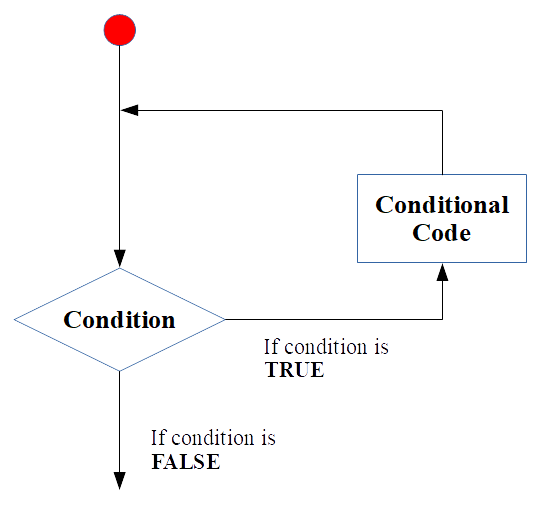
\includegraphics[width=0.4\linewidth]{skema_loop} 

}

\caption{Diagram umum loop (sumber: Primartha, 2018).}\label{fig:loop}
\end{figure}

\subsection{For Loop}\label{for-loop}

Mengulangi sebuah \emph{statement} atau sekelompok \emph{statement}
sebanyak nilai yang ditentukan di awal. Jadi operasi akan terus
dilakukan sampai dengan jumlah yang telah ditetapkan di awal atau dengan
kata lain tes kondisi (Jika jumlah pengulangan telah cukup) hanya akan
dilakukan di akhir. Secara sederhana bentuk dari \emph{for loop} dapat
dituliskan sebagai berikut:

\begin{Shaded}
\begin{Highlighting}[]
\ControlFlowTok{for}\NormalTok{ (value }\ControlFlowTok{in}\NormalTok{ vector)\{}
\NormalTok{  statements}
\NormalTok{\}}
\end{Highlighting}
\end{Shaded}

Berikut adalah contoh sintaks penerapan \emph{for loop}:

\begin{Shaded}
\begin{Highlighting}[]
\CommentTok{# Membuat vektor numerik}
\NormalTok{vektor <-}\StringTok{ }\KeywordTok{c}\NormalTok{(}\DecValTok{1}\OperatorTok{:}\DecValTok{5}\NormalTok{)}

\CommentTok{# loop }
\ControlFlowTok{for}\NormalTok{(i }\ControlFlowTok{in}\NormalTok{ vektor)\{}
  \KeywordTok{print}\NormalTok{(i)}
\NormalTok{\}}
\end{Highlighting}
\end{Shaded}

\begin{verbatim}
## [1] 1
## [1] 2
## [1] 3
## [1] 4
## [1] 5
\end{verbatim}

\emph{Loop} akan dimulai dari blok \emph{statement for} sampai dengan
\texttt{print(i)}. Berdasarkan \emph{loop} pada contoh tersebut,
\emph{loop} hanya dilakukan sebanyak 5 kali sesuai dengan jumlah vektor
yang ada.

\subsection{While Loop}\label{while-loop}

\emph{While loop} merupakan loop yang digunakan ketika kita telah
menetapkan \emph{stop condition} sebelumnya. Blok \emph{statement}/kode
yang sama akan terus dijalankan sampai \emph{stop condition} ini
tercapai. \emph{Stop condition} akan di cek sebelum melakukan proses
\emph{loop}. Berikut adalah pola dari \emph{while loop} dapat dituliskan
sebagai berikut:

\begin{Shaded}
\begin{Highlighting}[]
\ControlFlowTok{while}\NormalTok{ (test_expression)\{}
\NormalTok{  statement}
\NormalTok{\}}
\end{Highlighting}
\end{Shaded}

Berikut adalah contoh penerapan dari \emph{while loop}:

\begin{Shaded}
\begin{Highlighting}[]
\NormalTok{coba <-}\StringTok{ }\KeywordTok{c}\NormalTok{(}\StringTok{"Contoh"}\NormalTok{)}
\NormalTok{counter <-}\StringTok{ }\DecValTok{1}

\CommentTok{# loop}
\ControlFlowTok{while}\NormalTok{ (counter}\OperatorTok{<}\DecValTok{5}\NormalTok{)\{}
  \CommentTok{# print vektor}
  \KeywordTok{print}\NormalTok{(coba)}
  \CommentTok{# tambahkan nilai counter sehingga proses terus berlangsung sampai counter = 5 }
\NormalTok{  counter <-}\StringTok{ }\NormalTok{counter }\OperatorTok{+}\StringTok{ }\DecValTok{1}
\NormalTok{\}}
\end{Highlighting}
\end{Shaded}

\begin{verbatim}
## [1] "Contoh"
## [1] "Contoh"
## [1] "Contoh"
## [1] "Contoh"
\end{verbatim}

\emph{Loop} akan dimulai dari blok \emph{statement while} sampai dengan
\emph{counter} \textless{}- 1. \emph{Loop} hanya akan dilakukan
sepanjang nilai \emph{counter} \textless{} 5.

\subsection{Repeat Loop}\label{repeat-loop}

\emph{Repeat loop} akan menjalankan \emph{statement}/kode yang sama
berulang-ulang hingga \emph{stop condition} tercapai. Berikut adalah
pola dari \emph{repeat loop}.

\begin{Shaded}
\begin{Highlighting}[]
\ControlFlowTok{repeat}\NormalTok{ \{}
\NormalTok{  commands}
  \ControlFlowTok{if}\NormalTok{(condition)\{}
    \ControlFlowTok{break}
\NormalTok{  \}}
\NormalTok{\}}
\end{Highlighting}
\end{Shaded}

Berikut adalah contoh penerapan dari \emph{repeat loop}:

\begin{Shaded}
\begin{Highlighting}[]
\NormalTok{coba <-}\StringTok{ }\KeywordTok{c}\NormalTok{(}\StringTok{"contoh"}\NormalTok{)}
\NormalTok{counter <-}\StringTok{ }\DecValTok{1}
\ControlFlowTok{repeat}\NormalTok{ \{}
  \KeywordTok{print}\NormalTok{(coba)}
\NormalTok{  counter <-}\StringTok{ }\NormalTok{counter }\OperatorTok{+}\StringTok{ }\DecValTok{1}
  \ControlFlowTok{if}\NormalTok{(counter }\OperatorTok{<}\StringTok{ }\DecValTok{5}\NormalTok{)\{}
\ControlFlowTok{break}
\NormalTok{  \}}
\NormalTok{\}}
\end{Highlighting}
\end{Shaded}

\begin{verbatim}
## [1] "contoh"
\end{verbatim}

\emph{Loop} akan dimulai dari blok \emph{statement while} sampai dengan
\emph{break}. \emph{Loop} hanya akan dilakukan sepanjang nilai
\emph{counter} \textless{} 5. Hasil yang diperoleh berbeda dengan
\emph{while loop}, dimana kita memperoleh 4 buah kata ``contoh''. Hal
ini disebabkan karena \emph{repeat loop} melakukan pengecekan \emph{stop
condition} tidak di awal loop seperti \emph{while loop} sehingga
berapapun nilainya, selama nilainya sesuai dengan \emph{stop condition}
maka \emph{loop} akan dihentikan. Hal ini berbeda dengan \emph{while
loop} dimana proses dilakukan berulang-ulang sampai jumlahnya mendekati
\emph{stop condition}.

\subsection{Break}\label{break}

\emph{Break} sebenarnya bukan bagian dari \emph{loop}, namun sering
digunakan dalam \emph{loop}. \emph{Break} dapat digunakan pada
\emph{loop} manakala dirasa perlu, yaitu saat kondisi yang disyaratkan
pada \emph{break} tercapai.

Berikut adalah contoh penerapan \emph{break} pada beberapa jenis
\emph{loop}.

\begin{Shaded}
\begin{Highlighting}[]
\CommentTok{# for loop}
\NormalTok{a =}\StringTok{ }\KeywordTok{c}\NormalTok{(}\DecValTok{2}\NormalTok{,}\DecValTok{4}\NormalTok{,}\DecValTok{6}\NormalTok{,}\DecValTok{8}\NormalTok{,}\DecValTok{10}\NormalTok{,}\DecValTok{12}\NormalTok{,}\DecValTok{14}\NormalTok{)}
\ControlFlowTok{for}\NormalTok{(i }\ControlFlowTok{in}\NormalTok{ a)\{}
  \ControlFlowTok{if}\NormalTok{(i}\OperatorTok{>}\DecValTok{8}\NormalTok{)\{}
    \ControlFlowTok{break}
\NormalTok{  \}}
  \KeywordTok{print}\NormalTok{(i)}
\NormalTok{\}}
\end{Highlighting}
\end{Shaded}

\begin{verbatim}
## [1] 2
## [1] 4
## [1] 6
## [1] 8
\end{verbatim}

\begin{Shaded}
\begin{Highlighting}[]
\CommentTok{# while loop}
\NormalTok{a =}\StringTok{ }\DecValTok{2}
\NormalTok{b =}\StringTok{ }\DecValTok{4}
\ControlFlowTok{while}\NormalTok{(a}\OperatorTok{<}\DecValTok{7}\NormalTok{)\{}
  \KeywordTok{print}\NormalTok{(a)}
\NormalTok{  a =}\StringTok{ }\NormalTok{a }\OperatorTok{+}\DecValTok{1}
  \ControlFlowTok{if}\NormalTok{(b}\OperatorTok{+}\NormalTok{a}\OperatorTok{>}\DecValTok{10}\NormalTok{)\{}
    \ControlFlowTok{break}
\NormalTok{  \}}
\NormalTok{\}}
\end{Highlighting}
\end{Shaded}

\begin{verbatim}
## [1] 2
## [1] 3
## [1] 4
## [1] 5
## [1] 6
\end{verbatim}

\begin{Shaded}
\begin{Highlighting}[]
\CommentTok{# repeat loop}
\NormalTok{a =}\StringTok{ }\DecValTok{1}
\ControlFlowTok{repeat}\NormalTok{\{}
  \KeywordTok{print}\NormalTok{(a)}
\NormalTok{  a =}\StringTok{ }\NormalTok{a}\OperatorTok{+}\DecValTok{1}
  \ControlFlowTok{if}\NormalTok{(a}\OperatorTok{>}\DecValTok{6}\NormalTok{)\{}
    \ControlFlowTok{break}
\NormalTok{  \}}
\NormalTok{\}}
\end{Highlighting}
\end{Shaded}

\begin{verbatim}
## [1] 1
## [1] 2
## [1] 3
## [1] 4
## [1] 5
## [1] 6
\end{verbatim}

\section{Decision Making}\label{decision-making}

\emph{Decicion Making} atau sering disebut sebagai \emph{if then else
statement} merupakan bentuk percabagan yang digunakan manakala kita
ingin agar program dapat melakukan pengujian terhadap syarat kondisi
tertentu. Pada Table 5 disajikan daftar percabangan yang digunakan pada
\texttt{R}.

\textbf{Table 5} Daftar percabangan pada \texttt{R}

\begin{longtable}[]{@{}ll@{}}
\toprule
\begin{minipage}[b]{0.15\columnwidth}\raggedright\strut
\textbf{Statement}\strut
\end{minipage} & \begin{minipage}[b]{0.79\columnwidth}\raggedright\strut
\textbf{Keterangan}\strut
\end{minipage}\tabularnewline
\midrule
\endhead
\begin{minipage}[t]{0.15\columnwidth}\raggedright\strut
\emph{if statement}\strut
\end{minipage} & \begin{minipage}[t]{0.79\columnwidth}\raggedright\strut
\emph{if statement} hanya terdiri atas sebuah ekspresi \emph{Boolean},
dan diikuti satu atau lebih \emph{statement}\strut
\end{minipage}\tabularnewline
\begin{minipage}[t]{0.15\columnwidth}\raggedright\strut
\emph{if\ldots{}else statement}\strut
\end{minipage} & \begin{minipage}[t]{0.79\columnwidth}\raggedright\strut
\emph{if else statement} terdiri atas beberapa buah ekspresi
\emph{Boolean}. Ekspressi \emph{Boolean} berikutnya akan dijalankan jika
ekspresi *Boolan sebelumnya bernilai FALSE\strut
\end{minipage}\tabularnewline
\begin{minipage}[t]{0.15\columnwidth}\raggedright\strut
\emph{switch statement}\strut
\end{minipage} & \begin{minipage}[t]{0.79\columnwidth}\raggedright\strut
\emph{switch statement} digunakan untuk mengevaluasi sebuah variabel
beberapa pilihan\strut
\end{minipage}\tabularnewline
\bottomrule
\end{longtable}

\subsection{if statement}\label{if-statement}

Pola \emph{if statement} disajikan pada Figure \ref{fig:ifstatement}

\begin{figure}

{\centering 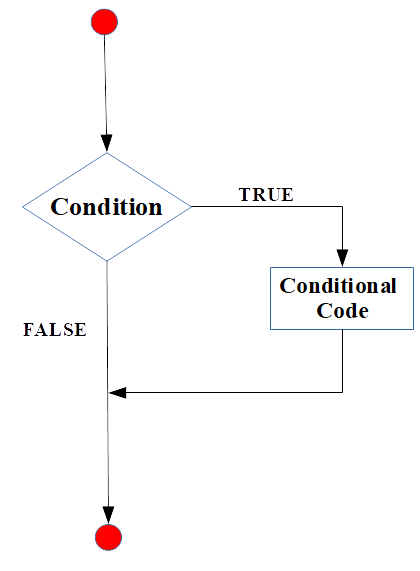
\includegraphics[width=0.4\linewidth]{ifstatement} 

}

\caption{Diagram if statement (sumber: Primartha, 2018).}\label{fig:ifstatement}
\end{figure}

Berikut adalah contoh penerapan \emph{if statement}:

\begin{Shaded}
\begin{Highlighting}[]
\NormalTok{x <-}\StringTok{ }\KeywordTok{c}\NormalTok{(}\DecValTok{1}\OperatorTok{:}\DecValTok{5}\NormalTok{)}
\ControlFlowTok{if}\NormalTok{(}\KeywordTok{is.vector}\NormalTok{(x))\{}
  \KeywordTok{print}\NormalTok{(}\StringTok{"x adalah sebuah vector"}\NormalTok{)}
\NormalTok{\}}
\end{Highlighting}
\end{Shaded}

\begin{verbatim}
## [1] "x adalah sebuah vector"
\end{verbatim}

\subsection{if else statement}\label{if-else-statement}

Pola dari \emph{if else statement} disajikan pada Figure
\ref{fig:ifelse}

\begin{figure}

{\centering 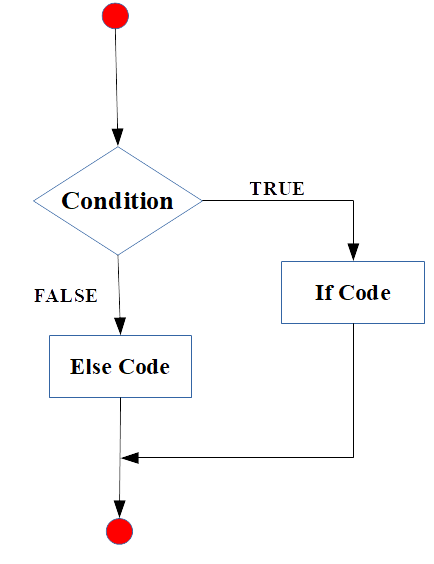
\includegraphics[width=0.4\linewidth]{ifelse} 

}

\caption{Diagram if else statement (sumber: Primartha, 2018).}\label{fig:ifelse}
\end{figure}

Berikut adalah contoh penerapan \emph{if else statement}:

\begin{Shaded}
\begin{Highlighting}[]
\NormalTok{x <-}\StringTok{ }\KeywordTok{c}\NormalTok{(}\StringTok{"Andi"}\NormalTok{,}\StringTok{"Iwan"}\NormalTok{, }\StringTok{"Adi"}\NormalTok{)}
\ControlFlowTok{if}\NormalTok{(}\StringTok{"Rina"} \OperatorTok\StringTok{ }\NormalTok{x)\{}
  \KeywordTok{print}\NormalTok{(}\StringTok{"Rina ditemukan"}\NormalTok{)}
\NormalTok{\} }\ControlFlowTok{else} \ControlFlowTok{if}\NormalTok{(}\StringTok{"Adi"} \OperatorTok\StringTok{ }\NormalTok{x)\{}
  \KeywordTok{print}\NormalTok{(}\StringTok{"Adi ditemukan"}\NormalTok{)}
\NormalTok{\} }\ControlFlowTok{else}\NormalTok{\{}
  \KeywordTok{print}\NormalTok{(}\StringTok{"tidak ada yang ditemukan"}\NormalTok{)}
\NormalTok{\}}
\end{Highlighting}
\end{Shaded}

\begin{verbatim}
## [1] "Adi ditemukan"
\end{verbatim}

\subsection{switch statement}\label{switch-statement}

Pola dari \emph{switch statement} disajikan pada Figure \ref{fig:switch}

\begin{figure}

{\centering 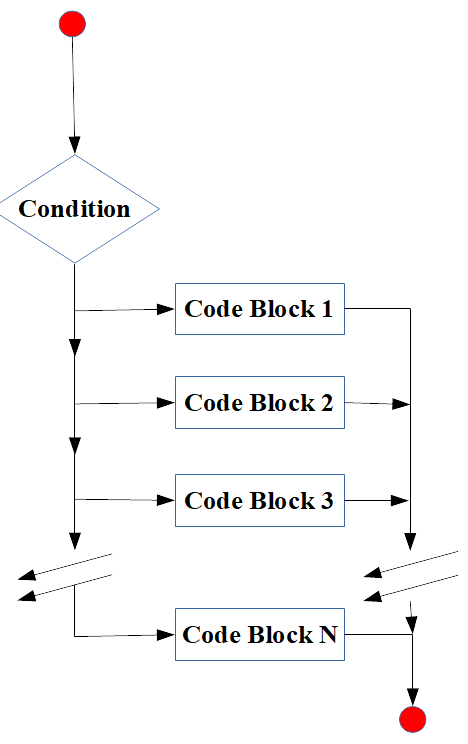
\includegraphics[width=0.4\linewidth]{switch} 

}

\caption{Diagram switch statement (sumber: Primartha, 2018).}\label{fig:switch}
\end{figure}

Berikut adalah contoh penerapan \emph{switch statement}:

\begin{Shaded}
\begin{Highlighting}[]
\NormalTok{y =}\StringTok{ }\DecValTok{3}

\NormalTok{x =}\StringTok{ }\ControlFlowTok{switch}\NormalTok{(}
\NormalTok{  y,}
  \StringTok{"Selamat Pagi"}\NormalTok{,}
  \StringTok{"Selamat Siang"}\NormalTok{,}
  \StringTok{"Selamat Sore"}\NormalTok{,}
  \StringTok{"Selamat Malam"}
\NormalTok{)}

\KeywordTok{print}\NormalTok{(x)}
\end{Highlighting}
\end{Shaded}

\begin{verbatim}
## [1] "Selamat Sore"
\end{verbatim}

\section{Fungsi}\label{fungsi}

Fungsi merupakan sekumpulan instruksi atau \emph{statement} yang dapat
melakukan tugas khusus. Sebagai contoh fungsi perkalian untuk
menyelesaikan operasi perkalian, fungsi pemangkatan hanya untuk operasi
pemangkatan, dll.

Pada \texttt{R} terdapat 2 jenis fungsi, yaitu: \emph{build in fuction}
dan \emph{user define function}. \emph{build in fnction} merupakan
fungsi bawaan \texttt{R} saat pertama kita menginstall \texttt{R}.
Contohnya adalah \texttt{mean()}, \texttt{sum()}, \texttt{ls()},
\texttt{rm()}, dll. Sedangkan \emph{user define fuction} merupakan
fungsi-fungsi yang dibuat sendiri oleh pengguna.

Fungsi-fungsi buatan pengguna haruslah dideklarasikan (dibuat) terlebih
dahulu sebelum dapat dijalankan. Pola pembentukan fungsi adalah sebagai
berikut:

\begin{Shaded}
\begin{Highlighting}[]
\NormalTok{function_name <-}\StringTok{ }\ControlFlowTok{function}\NormalTok{(argument_}\DecValTok{1}\NormalTok{, argument_}\DecValTok{2}\NormalTok{, ...)\{}
  \ControlFlowTok{function}\NormalTok{ body}
\NormalTok{\}}
\end{Highlighting}
\end{Shaded}

\begin{quote}
\textbf{Note: }

\begin{itemize}
\tightlist
\item
  \textbf{function\_name} : Nama dari fungsi \texttt{R}. \texttt{R} akan
  menyimpan fungsi tersebut sebagai objek
\item
  \textbf{argument\_1, argument\_2,\ldots{}} : \emph{Argument} bersifat
  opsional (tidak wajib). \emph{Argument} dapat digunakan untuk memberi
  inputan kepada fungsi
\item
  \textbf{function body} : Merupakan inti dari fungsi. Fuction body
  dapat terdiri atas 0 statement (kosong) hingga banyak statement.
\item
  \textbf{return} : Fungsi ada yang memiliki \emph{output} atau
  \emph{return value} ada juga yang tidak. Jika fungsi memiliki
  \emph{return value} maka \emph{return value} dapat diproses lebih
  lanjut
\end{itemize}
\end{quote}

Berikut adalah contoh penerapan \emph{user define function}:

\begin{Shaded}
\begin{Highlighting}[]
\CommentTok{# Fungsi tanpa argument}
\NormalTok{bilang <-}\StringTok{ }\ControlFlowTok{function}\NormalTok{()\{}
  \KeywordTok{print}\NormalTok{(}\StringTok{"Hello World!!"}\NormalTok{)}
\NormalTok{\}}

\CommentTok{# Print}
\KeywordTok{bilang}\NormalTok{()}
\end{Highlighting}
\end{Shaded}

\begin{verbatim}
## [1] "Hello World!!"
\end{verbatim}

\begin{Shaded}
\begin{Highlighting}[]
\CommentTok{# Fungsi dengan argumen}
\NormalTok{tambah <-}\StringTok{ }\ControlFlowTok{function}\NormalTok{(a,b)\{}
  \KeywordTok{print}\NormalTok{(a}\OperatorTok{+}\NormalTok{b)}
\NormalTok{\}}

\CommentTok{# Print}
\KeywordTok{tambah}\NormalTok{(}\DecValTok{5}\NormalTok{,}\DecValTok{3}\NormalTok{)}
\end{Highlighting}
\end{Shaded}

\begin{verbatim}
## [1] 8
\end{verbatim}

\begin{Shaded}
\begin{Highlighting}[]
\CommentTok{# Fungsi dengan return value}
\NormalTok{kali <-}\StringTok{ }\ControlFlowTok{function}\NormalTok{(a,b)\{}
  \KeywordTok{return}\NormalTok{(a}\OperatorTok{*}\NormalTok{b)}
\NormalTok{\}}

\CommentTok{# Print}
\KeywordTok{kali}\NormalTok{(}\DecValTok{4}\NormalTok{,}\DecValTok{3}\NormalTok{)}
\end{Highlighting}
\end{Shaded}

\begin{verbatim}
## [1] 12
\end{verbatim}

\section{Referensi}\label{referensi-1}

\begin{enumerate}
\def\labelenumi{\arabic{enumi}.}
\tightlist
\item
  Primartha, R. 2018. \textbf{Belajar Machine Learning Teori dan
  Praktik}. Penerbit Informatika : Bandung.
\item
  Rosadi,D. 2016. \textbf{Analisis Statistika dengan R}. Gadjah Mada
  University Press: Yogyakarta.
\item
  STHDA. \textbf{Easy R Programming Basics}.
  \url{http://www.sthda.com/english/wiki/easy-r-programming-basics}
\item
  Venables, W.N. Smith D.M. and R Core Team. 2018. \textbf{An
  Introduction to R}. R Manuals.
\item
  The R Core Team. 2018. \textbf{R: A Language and Environment for
  Statistical Computing}. R Manuals.
\end{enumerate}

\chapter{Manajemen Data R}\label{manajemen-data-r}

Data manajemen merupakan bagian penting dalam setiap proses analisa
data. Proses import dan eksport data pada berbagai format penting untuk
dipelajari. Selain itu, proses perapihan data sebelum analisa menjadi
bagian yang harus ada pada awal proses analisa. Proses-proses tersebut
akan kita ulas secara mendalam pada \emph{chapter} ini.\emph{Chapter}
ini juga akan membahas bagaimana kita dapat melakukan sejumlah
manipulasi data untuk memperoleh informasi lebih yang terkandung pada.

\section{Import File}\label{import-file}

Pada sesi bagian ini penulis akan menjelaskan cara mengimport file pada
\texttt{R}. File yang diimport ke dalam \texttt{R} terdiri atas file
yang sering digunakan pada saat akan melakukan analisis data, antara
lain: TXT, CSv, Excel, SPSS, SAS, dan STATA.

Pada bagian ini akan dijelaskan pula bagaimana melakukan import data
menggunakan library \texttt{readr} serta kelebihan dari metode import
data yang digunakan. Berikut adalah cara mengimport data berbagai format
pada \texttt{R}.

\begin{quote}
\textbf{Note: } Pastikan kita telah mengatur lokasi \emph{working
directory} pada tempat dimana lokasi file yang akan kita baca berada
untuk mempermudah dalam melakukan import file.
\end{quote}

\subsection{Import File Menggunakan Fungsi Bawaan
R}\label{import-file-menggunakan-fungsi-bawaan-r}

Fungsi bawaan \texttt{R} secara umum hanya dapat membaca data dengan
format TXT dan CSV. Pada \texttt{RStudio} fungsi ini bertambah dengan
adanya library tambahan yang telah terinstall di \texttt{RStudio} untuk
membaca file dengan format EXCEL, SPSS, SAS dan STATA.

Secara umum fungsi yang digunakan untuk membaca data dengan format tabel
seperti TXT dan CSV adalah fungsi\texttt{read.table()}. Berikut adalah
list fungsi dasar lainnya untuk membaca file dengan format TXT dan CSV
pada \texttt{R}:

\begin{itemize}
\tightlist
\item
  \textbf{read.csv()}: untuk membaca file dengan format \emph{comma
  separated value}(``.csv'').
\item
  \textbf{read.csv2()}: varian yang digunakan jika pada file ``.csv''
  yang akan dibaca mengandung koma (``,'') sebagai desimal dan semicolon
  (``;'') sebagai pemisah antar variabel atau kolom.
\item
  \textbf{read.delim()}: untuk membaca file dengan format
  \emph{tab-separated value}(``.txt'').
\item
  \textbf{read.delim2()}: membaca file dengan format ``.txt'' dengan
  tanda koma (``,'') sebagai penujuk bilangan desimal.
\end{itemize}

Masing-masing fungsi diatas dapat dituliskan kedalam \texttt{R} dengan
format sebagai berikut:

\begin{Shaded}
\begin{Highlighting}[]
\CommentTok{# Membaca tabular data pada  R}
\KeywordTok{read.table}\NormalTok{(file, }\DataTypeTok{header =} \OtherTok{FALSE}\NormalTok{, }\DataTypeTok{sep =} \StringTok{""}\NormalTok{, }\DataTypeTok{dec =} \StringTok{"."}\NormalTok{)}
\CommentTok{# Membaca"comma separated value" files (".csv")}
\KeywordTok{read.csv}\NormalTok{(file, }\DataTypeTok{header =} \OtherTok{TRUE}\NormalTok{, }\DataTypeTok{sep =} \StringTok{","}\NormalTok{, }\DataTypeTok{dec =} \StringTok{"."}\NormalTok{, ...)}
\CommentTok{# atau gunakan read.csv2 jika tanda desimal pada data adalah "," dan pemisah kolom adalah ";"}
\KeywordTok{read.csv2}\NormalTok{(file, }\DataTypeTok{header =} \OtherTok{TRUE}\NormalTok{, }\DataTypeTok{sep =} \StringTok{";"}\NormalTok{, }\DataTypeTok{dec =} \StringTok{","}\NormalTok{, ...)}
\CommentTok{# MembacaTAB delimited files}
\KeywordTok{read.delim}\NormalTok{(file, }\DataTypeTok{header =} \OtherTok{TRUE}\NormalTok{, }\DataTypeTok{sep =} \StringTok{"}\CharTok{\textbackslash{}t}\StringTok{"}\NormalTok{, }\DataTypeTok{dec =} \StringTok{"."}\NormalTok{, ...)}
\KeywordTok{read.delim2}\NormalTok{(file, }\DataTypeTok{header =} \OtherTok{TRUE}\NormalTok{, }\DataTypeTok{sep =} \StringTok{"}\CharTok{\textbackslash{}t}\StringTok{"}\NormalTok{, }\DataTypeTok{dec =} \StringTok{","}\NormalTok{, ...)}
\end{Highlighting}
\end{Shaded}

\begin{quote}
\textbf{Note: }

\begin{itemize}
\tightlist
\item
  \textbf{file}: nama file diakhiri dengan format file (misal:
  ``nama\_file.txt'') yang akan di import ke dalam file. Dapat pula
  diisi lokasi file tersebut berada, misal:(C:/Users/My
  PC/Documents/nama\_file.txt atau .csv)
\item
  \textbf{sep}: pemisah antar kolom. ``\t'' digunakan untuk
  tab-delimited file.
\item
  \textbf{header}: nilai logik. jika TRUE, maka \texttt{read.table()}
  akan menganggap bahwa file yang akan dibaca pada baris pertama file
  merupakan header data.
\item
  \textbf{dec}: karakter yang digunakan sebagai penunjuk desimal pada
  data.
\end{itemize}
\end{quote}

Untuk info lebih lanjut terkait fungsi-fungsi tersebut dan contoh
bagaimana menggunakannya, pembaca dapat mengakses fitur batuan dari
fungsi tersebut menggunakan sintaks berikut:

\begin{Shaded}
\begin{Highlighting}[]
\CommentTok{# mengakses menu bantuan}
\NormalTok{?read.table}
\NormalTok{?read.csv}
\NormalTok{?read.csv2}
\NormalTok{?read.delim}
\NormalTok{?read.delim2}
\end{Highlighting}
\end{Shaded}

Misalkan penulis memiliki data pada file bernama ``mtcars.csv'' dengan
desimal berupa titik pada datanya. Penulsi ingin membaca file tersebut,
maka penulis akan menuliskan sintaks berikut:

\begin{Shaded}
\begin{Highlighting}[]
\NormalTok{data <-}\StringTok{ }\KeywordTok{read.csv}\NormalTok{(}\StringTok{"mtcars.csv"}\NormalTok{)}
\end{Highlighting}
\end{Shaded}

Secara default perintah tersebut akan membaca baris pertama data sebagai
header serta data berupa karakter menjadi factor. Untuk mencegah agar
data berupa karakter menjadi faktor, perintah tersebut dapat ditambahkan
parameter \texttt{stringAsFactor\ =\ FALSE}.

Kita juga dapat memilih file yang akan kita baca secara interakti. Misal
pada \emph{working directory} terdapat beberapa file yang akan kita
baca. Kita ingin melihat file dengan format tertentu yang hendak kita
baca, namun kita malas mengecek file explorer pada windows. Untuk
mengatasi masalah tersebut, kita dapat menggunakan fungsi
\texttt{file.choose()} pada \texttt{R}. Fungsi tersebut akan menampilkan
jendela windows explores sehingga kita dapat memilih file apa yang
hendak dibaca. Berikut adalah contoh penerapannya:

\begin{Shaded}
\begin{Highlighting}[]
\NormalTok{data <-}\StringTok{ }\KeywordTok{read.csv}\NormalTok{(}\KeywordTok{file.choose}\NormalTok{())}
\end{Highlighting}
\end{Shaded}

\begin{quote}
\textbf{Note: } pastikan format file yang dibaca sama dengan fungsi
import yang digunakan.
\end{quote}

Kita juga dapat membaca file dari internet. Untuk melakukannya kit hanya
perlu meng-copy url file tersebut. Berikut adalah contoh file yang
dibaca dari internet:

\begin{Shaded}
\begin{Highlighting}[]
\CommentTok{# Membaca file dari internet}
\NormalTok{data <-}\StringTok{ }\KeywordTok{read.delim}\NormalTok{(}\StringTok{"http://www.sthda.com/upload/boxplot_format.txt"}\NormalTok{)}

\CommentTok{# mengecek 6 observasi awal}
\KeywordTok{head}\NormalTok{(data)}
\end{Highlighting}
\end{Shaded}

\begin{verbatim}
##    Nom variable Group
## 1 IND1       10     A
## 2 IND2        7     A
## 3 IND3       20     A
## 4 IND4       14     A
## 5 IND5       14     A
## 6 IND6       12     A
\end{verbatim}

\subsection{Membaca File CSV dan TXT Menggunakan Library
readr}\label{membaca-file-csv-dan-txt-menggunakan-library-readr}

Pada bagian sebelumnya kita telah belajar bagaimana cara membaca file
dengan format CSV dan TXT menggunakan paket dasar \texttt{R}. Pada
bagian ini penulis akan menjelaskan bagaimana cara membaca file dengan
format TXT dan CSV pada \texttt{R} menggunakan paket \texttt{readr}.

\texttt{readr} dikembangkan oleh Hadley Wickham. paket \texttt{readr}
memberikan solusi cepat dan ramah untuk membaca delimited file ke dalam
\texttt{R}.

Dibandingkan dengan paket dasar \texttt{R}, \texttt{readr} memiliki
kelebihan sebagai berikut:

\begin{itemize}
\tightlist
\item
  Mampu membaca file 10x lebih cepat dibandingkan pada paket bawaan
  \texttt{R}.
\item
  Menampilkan \emph{progress bar} yang bermanfaat jika proses pemuatan
  berlangsung agak lama.
\item
  semua fungsi bekerja dengan cara yang persis sama dengan paket bawaan
  \texttt{R}.
\end{itemize}

Untuk dapat menggunakan \texttt{readr}, kita perlu menginstall paketnya
terlebih dahulu. Untuk melakukannya jalankan sintaks berikut:

\begin{Shaded}
\begin{Highlighting}[]
\CommentTok{# Menginstall paket}
\KeywordTok{install.packages}\NormalTok{(}\StringTok{"readr"}\NormalTok{)}

\CommentTok{# Memuat paket}
\KeywordTok{library}\NormalTok{(readr)}
\end{Highlighting}
\end{Shaded}

Berikut adalah format bebrapa fungsi yang dapat digunakan:

\begin{Shaded}
\begin{Highlighting}[]
\CommentTok{# Fungsi umum (membaca TXT dan CSV) dapat juga membaca flat file dan tsv}
\KeywordTok{read_delim}\NormalTok{(file, delim, }\DataTypeTok{col_names =} \OtherTok{TRUE}\NormalTok{)}
\CommentTok{# Membaca comma (",") separated values}
\KeywordTok{read_csv}\NormalTok{(file, }\DataTypeTok{col_names =} \OtherTok{TRUE}\NormalTok{)}
\CommentTok{# Membaca semicolon (";") separated values}
\KeywordTok{read_csv2}\NormalTok{(file, }\DataTypeTok{col_names =} \OtherTok{TRUE}\NormalTok{)}
\CommentTok{# Membaca tab separated values}
\KeywordTok{read_tsv}\NormalTok{(file, }\DataTypeTok{col_names =} \OtherTok{TRUE}\NormalTok{)}
\end{Highlighting}
\end{Shaded}

\begin{quote}
\textbf{Note: }

\begin{itemize}
\tightlist
\item
  \textbf{file}: path file, koneksi atau raw vector. File yang
  berakhiran .gz, .bz2, .xz, atau .zip akan secara otomatis tidak
  terkompresi. File yang dimulai dengan ``http: //'', ``https: //'',
  ``ftp: //'', atau ``ftps: //'' akan diunduh secara otomatis. File gz
  jarak jauh juga dapat diunduh \& didekompresi secara otomatis.
\item
  \textbf{delim}: karakter yang membatasi tiap nilai pada file.
\item
  \textbf{col\_names}: nilai logik. Jika TRUE, maka baris pertama akan
  menjadi header.
\end{itemize}
\end{quote}

Berikut adalah contoh bagaimana cara membaca file menggunakan fungsi
pada paket \texttt{readr}:

\begin{Shaded}
\begin{Highlighting}[]
\CommentTok{# Membaca file lokal}
\NormalTok{data <-}\StringTok{ }\KeywordTok{read_csv}\NormalTok{(}\StringTok{"mtcars.csv"}\NormalTok{)}

\CommentTok{# atau}
\NormalTok{data <-}\StringTok{ }\KeywordTok{read_csv}\NormalTok{(}\KeywordTok{file.choose}\NormalTok{())}

\CommentTok{# Membaca dari internet}
\NormalTok{data <-}\StringTok{ }\KeywordTok{read_tsv}\NormalTok{(}\StringTok{"http://www.sthda.com/upload/boxplot_format.txt"}\NormalTok{)}
\end{Highlighting}
\end{Shaded}

Kita juga dapat menspesifikasi jenis data pada kolom yang akan dibaca.
Keuntungan dari penentuan jenis kolom (tipe data) akan memastikan data
yang telah dibaca tidak salah berdasarkan jenis data pada masing-masing
kolom.

Beberapa format jenis kolom yang tersedia pada \texttt{readr} adalah
sebagi berikut:

\begin{itemize}
\tightlist
\item
  \textbf{col\_integer()}: untuk menentukan integer (alias = ``i'').
\item
  \textbf{col\_double()}: untuk menentukan kolom sebagai jenis data
  double (alias = ``d'').
\item
  \textbf{col\_logical()}: untuk menentukan variabel logis (alias =
  ``l'').
\item
  \textbf{col\_character()}: meninggalkan string apa adanya.Tidak
  mengonversinya menjadi faktor (alias = ``c'').
\item
  \textbf{col\_factor()}: untuk menentukan variabel faktor (atau
  pengelompokan) (alias = ``f'')
\item
  \textbf{col\_skip()}: untuk mengabaikan kolom (alias = ``-'' atau
  ``\_``)
\item
  \textbf{col\_date()} (alias = ``D''), \textbf{col\_datetime()} (alias
  = ``T'') dan \textbf{col\_time()} (``t'') untuk menentukan tanggal,
  waktu tanggal, dan waktu.
\end{itemize}

Berikut adalah contoh penerapannya:

\begin{Shaded}
\begin{Highlighting}[]
\NormalTok{data <-}\StringTok{ }\KeywordTok{read_csv}\NormalTok{(}\StringTok{"my_file.csv"}\NormalTok{, }\DataTypeTok{col_types =} \KeywordTok{cols}\NormalTok{(}
  \DataTypeTok{x =} \StringTok{"i"}\NormalTok{, }\CommentTok{# kolom integer}
  \DataTypeTok{treatment =} \StringTok{"c"} \CommentTok{# kolom karakter/string}
\NormalTok{))}
\end{Highlighting}
\end{Shaded}

\subsection{Import File Excel Pada R}\label{import-file-excel-pada-r}

Keunggulan penggunaan excel sebagai format penyimpan data adalah kita
dapat menyimpan banyak data dan memisahkannya pada lembar (\emph{sheet})
yang berbeda sebagai suatu data yang independen dibandingkan pembacaan
pada file csv yang hanya berisikan satu tabel data saja tiap file.

Pada \texttt{R} kita dapat melakukan pembacaan file menggunakan berbagai
macam cara seperti menggunakan paket bawaan \texttt{R} maupun
menggunakan library yang perlu kita install. Berikut adalah beberapa
cara membaca file excel pada \texttt{R}.

\begin{enumerate}
\def\labelenumi{\alph{enumi}.}
\item
  Mengkonversi terlebih dahulu satu sheet excel yang akan kita baca
  menjadi format ``.csv'' maupun ``.txt'' sehingga dapat dibaca seperti
  pada sub-bab 3.1.1.
\item
  Menyalin data dari excel dan mengimport data pada \texttt{R}.
\end{enumerate}

Cara ini sedikit mirip dengan cara sebelumnya, dimana kita perlu membuka
file excel dan melakukan \textbf{select} dan \textbf{copy} (ctrl+c)
tabel data yang hendak dibaca. Data tersebut selanjutnya akan tersimpan
pada \textbf{clipboard}.

Data yang telah tersalin selanjutnya diimport ke \texttt{R} dengan
mengetikkan sintaks berikut:

\begin{Shaded}
\begin{Highlighting}[]
\NormalTok{data <-}\StringTok{ }\KeywordTok{read.table}\NormalTok{(}\DataTypeTok{file=} \StringTok{"clipboard"}\NormalTok{,}
                   \DataTypeTok{sep =} \StringTok{"}\CharTok{\textbackslash{}t}\StringTok{"}\NormalTok{, }\DataTypeTok{header =} \OtherTok{TRUE}\NormalTok{)}
\end{Highlighting}
\end{Shaded}

Cara ini merupakan cara yang paling sering penulis gunakan. Kelemahan
penggunaan cara ini adalah ketika kita melakukan proses \textbf{select}
dan \textbf{copy} (ctrl+c) tabel yang jumlahnya sangat banyak dan
terdapat teks-teks penjelasan terkait tabel data pada lembar kerja excel
yang tidak ingin kita sertakan akan memakan waktu yang lebih lama pada
proses \textbf{select}.

\begin{enumerate}
\def\labelenumi{\alph{enumi}.}
\setcounter{enumi}{2}
\tightlist
\item
  Mengimport data menggunakan library readxl.
\end{enumerate}

Paket \texttt{readxl}, yang dikembangkan oleh Hadley Wickham, dapat
digunakan untuk dengan mudah mengimpor file Excel (xls \textbar{} xlsx)
ke \texttt{R} tanpa ada ketergantungan eksternal.

Untuk dapat menggunakan library \texttt{readxl} kita harus
menginstallnya terlebih dahulu menggunakan sintaks berikut:

\begin{Shaded}
\begin{Highlighting}[]
\CommentTok{# Instal paket}
\KeywordTok{install.packages}\NormalTok{(}\StringTok{"readxl"}\NormalTok{)}

\CommentTok{# memuat paket}
\KeywordTok{library}\NormalTok{(readxl)}
\end{Highlighting}
\end{Shaded}

Berikut adalah contoh cara mengimport data dengan format xls atau xlsx
pada \texttt{R}.

\begin{Shaded}
\begin{Highlighting}[]
\CommentTok{# Tentukan sheet dengan nama sheet pada file}
\NormalTok{data <-}\StringTok{ }\KeywordTok{read_excel}\NormalTok{(}\StringTok{"my_file.xlsx"}\NormalTok{, }\DataTypeTok{sheet =} \StringTok{"data"}\NormalTok{)}

\CommentTok{# Tentukan sheet berdasarkan indeks sheet}
\NormalTok{data <-}\StringTok{ }\KeywordTok{read_excel}\NormalTok{(}\StringTok{"my_file.xlsx"}\NormalTok{, }\DataTypeTok{sheet =} \DecValTok{2}\NormalTok{) }\CommentTok{# membaca sheet ke-2}
\end{Highlighting}
\end{Shaded}

\begin{enumerate}
\def\labelenumi{\alph{enumi}.}
\setcounter{enumi}{3}
\tightlist
\item
  Mengimport data menggunakan library xlsx
\end{enumerate}

Paket \texttt{xlsx}, solusi berbasis \texttt{java}, adalah salah satu
paket \texttt{R} yang ampuh untuk membaca, menulis, dan memformat file
Excel. Untuk dapat menggunakannya kita harus menginstall dan memuatnya
terlebih dahulu. Berikut sintaks yang digunakan:

\begin{Shaded}
\begin{Highlighting}[]
\CommentTok{# Menginstall paket}
\KeywordTok{install.packages}\NormalTok{(}\StringTok{"xlsx"}\NormalTok{)}

\CommentTok{# Memuat paket}
\KeywordTok{library}\NormalTok{(xlsx)}
\end{Highlighting}
\end{Shaded}

Terdapat dua buah fungsi yang disediakan pada paket tersebut yaitu
\texttt{read.xlsx()} dan \texttt{read.xlsx2()}. Perbedaan keduanya
adalah \texttt{read.xlsx2()} digunakan pada file data dengan ukuran yang
besar serta proses pembacaan data yang lebih cepat dibandingkan dengan
\texttt{read.xlsx()}. Fromat yang digunakan untuk kedua fungsi tersebut
disajikan sebagai berikut:

\begin{Shaded}
\begin{Highlighting}[]
\KeywordTok{read.xlsx}\NormalTok{(file, sheetIndex, }\DataTypeTok{header=}\OtherTok{TRUE}\NormalTok{)}
\KeywordTok{read.xlsx2}\NormalTok{(file, sheetIndex, }\DataTypeTok{header=}\OtherTok{TRUE}\NormalTok{)}
\end{Highlighting}
\end{Shaded}

\begin{quote}
\textbf{Note: }

\begin{itemize}
\tightlist
\item
  \textbf{file}: nama atau lokasi file berada
\item
  \textbf{sheetIndex}: Indeks dari sheet yang hendak dibaca
\item
  \textbf{header}: nilai logik. Jika bernilai TRUE, maka baris pertama
  dari sheet menjadi header.
\end{itemize}
\end{quote}

Berikut adalah contoh penggunaanya:

\begin{Shaded}
\begin{Highlighting}[]
\NormalTok{data <-}\StringTok{ }\KeywordTok{read.xlsx}\NormalTok{(}\KeywordTok{file.choose}\NormalTok{(), }\DecValTok{1}\NormalTok{) }\CommentTok{# membaca sheet 1}
\end{Highlighting}
\end{Shaded}

\begin{quote}
\textbf{Note: } kita juga dapat membaca file dari internet seperti pada
sub-bab 3.1.1.
\end{quote}

\subsection{Membaca File Dari Format Aplikasi
Statistik}\label{membaca-file-dari-format-aplikasi-statistik}

Untuk membaca file yang berasal dari format aplikasi statistik seperti
SPSS, SAS, dan STATA kita perlu menginstal dan memuat paket-paket yang
dibutuhkan sesuai dengan file yang akan kita install. Berikut adalah
sintaks bagaimana cara mengimport file dari berbagai format aplikasi
statistik.

\begin{Shaded}
\begin{Highlighting}[]
\CommentTok{# membaca file SPSS}
\KeywordTok{install.packages}\NormalTok{(}\StringTok{"Hmisc"}\NormalTok{) }\CommentTok{# menginstall paket}
\KeywordTok{library}\NormalTok{(Hmisc) }\CommentTok{# memuat paket}
\CommentTok{# simpan SPSS dataset pada transport format}
\NormalTok{get file=}\StringTok{'c:\textbackslash{}mydata.sav'}\NormalTok{.}
\NormalTok{export outfile=}\StringTok{'c:\textbackslash{}mydata.por'}\NormalTok{. }
\NormalTok{data <-}\StringTok{ }\KeywordTok{spss.get}\NormalTok{(}\StringTok{"c:\textbackslash{}mydata.por"}\NormalTok{, }\DataTypeTok{use.value.labels=} \OtherTok{TRUE}\NormalTok{) }
\CommentTok{# use.value.labels digunakan untuk mengubah label menjadi factor}


\CommentTok{# membaca file SAS}
\KeywordTok{install.packages}\NormalTok{(}\StringTok{"Hmisc"}\NormalTok{) }\CommentTok{# menginstall paket}
\KeywordTok{library}\NormalTok{(Hmisc) }\CommentTok{# memuat paket}
\CommentTok{# simpan SAS dataset pada transport format}
\NormalTok{libname out xport }\StringTok{'c:/mydata.xpt'}\NormalTok{;}
\NormalTok{data out.mydata;}
\NormalTok{set sasuser.mydata;}
\NormalTok{run;}
\NormalTok{data <-}\StringTok{ }\KeywordTok{sasxport.get}\NormalTok{(}\StringTok{"c:/mydata.xpt"}\NormalTok{) }
\CommentTok{# Variabel yang berupa karakter akan dikonversi menjadi factor}


\CommentTok{# membaca file STATA}
\KeywordTok{install.packages}\NormalTok{(}\StringTok{"foreign"}\NormalTok{) }\CommentTok{# menginstall paket}
\KeywordTok{library}\NormalTok{(foreign) }\CommentTok{# memuat paket}
\NormalTok{data <-}\StringTok{ }\KeywordTok{read.dta}\NormalTok{(}\StringTok{"c:/mydata.dta"}\NormalTok{)}
\end{Highlighting}
\end{Shaded}

\section{Eksport File}\label{eksport-file}

Setelah kita melakukan analisa dan telah memperoleh hasil yang kita
inginkan dan memperoleh data frame berupa hasil prediksi suatu model
atau data yang telah dibersihakan, kita ingin melakukan pelaporan dalam
bentuk file dengan format seperti EXCEL, CSV atau TXT. Untuk
melakukannya kita perlu melakukan eksport data yang telah dihasilkan.

Pada bagian ini penulis akan menjelaskan bagaimana cara mengeksport data
dari \texttt{R} kedalam format TXT, CSV, maupun EXCEL. Sebenarnya
\texttt{R} memungkinkan untuk melakukan eksport dalam format lain
seperti RDA maupun RDS yang tidak dibahas dalam buku ini karena berada
diluar lingkup buku ini.

\subsection{Eksport Data Menjadi Format TXT dan
CSV}\label{eksport-data-menjadi-format-txt-dan-csv}

Terdapat dua cara untuk melakukan ekport data dari \texttt{R} menjadi
format TXT atau CSV, yaitu melalui paket dasar \texttt{R} maupun
menggunakan library \texttt{readr}. Kedua cara tersebut memiliki
sejumlah kemiripan dari segi fungsi, namun berbeda dari segi kecepatan
eksport.

Fungsi dasar yang digunakan pada \texttt{R} untuk melakukan eksport file
kedalam format TXT dan CSv adalah \texttt{write.tabel()}. Format umum
yang digunakan adalah sebagai berikut:

\begin{Shaded}
\begin{Highlighting}[]
\KeywordTok{write.table}\NormalTok{(x, file, }\DataTypeTok{sep=} \StringTok{" "}\NormalTok{, }\DataTypeTok{dec =} \StringTok{","}\NormalTok{,}
            \DataTypeTok{row.names =} \OtherTok{TRUE}\NormalTok{, }\DataTypeTok{col.names =} \OtherTok{TRUE}\NormalTok{)}
\end{Highlighting}
\end{Shaded}

\begin{quote}
\textbf{Note: }

\begin{itemize}
\tightlist
\item
  \textbf{x}: matriks atau data frame yang akan ditulis.
\item
  \textbf{file}: karakter yang menentukan nama file yang dihasilkan.
\item
  \textbf{sep}: string pemisah bidang atau kolom, mis., sep = ``~t''
  (untuk nilai yang dipisahkan tab).
\item
  \textbf{dec}: string yang akan digunakan sebagai pemisah desimal.
  Standarnya adalah ``.''.
\item
  \textbf{row.names}: nilai logik yang menunjukkan apakah nama baris x
  harus ditulis bersama dengan x, atau vektor karakter nama baris yang
  akan ditulis.
\item
  \textbf{col.names}: baik nilai logik yang menunjukkan apakah nama
  kolom x harus ditulis bersama dengan x, atau vektor karakter nama
  kolom yang akan ditulis. Jika \texttt{col.names\ =\ NA} dan
  \texttt{row.names\ =\ TRUE} ditambahkan nama kolom kosong, yang
  merupakan konvensi yang digunakan untuk file CSV untuk dibaca oleh
  spreadsheet.
\end{itemize}
\end{quote}

Selain menggunakan fungsi tersebut, untuk eksport ke dalam format CSV
juga dapa menggunakan fungsi \texttt{write.csv()} atau
\texttt{write.csv2()}. Berikut adalah format yang digunakan:

\begin{Shaded}
\begin{Highlighting}[]
\KeywordTok{write.csv}\NormalTok{(data, }\DataTypeTok{file=}\StringTok{"data.csv"}\NormalTok{)}
\KeywordTok{write.csv2}\NormalTok{(data, }\DataTypeTok{file=}\StringTok{"data.csv"}\NormalTok{)}
\end{Highlighting}
\end{Shaded}

Secara penampakan kedua fungsi tersebut pada dasarnya sama dengan fungsi
\texttt{write.table()}, bedanya adalah kedua fungsi tersebut spesifik
digunakan untuk eksport file kedalam format CSV.

\begin{quote}
\textbf{Note: }

\begin{itemize}
\tightlist
\item
  \textbf{write.csv()} menggunakan ``.'' sebagai titik desimal serta
  ``,'' sebagai pemisah antar kolom data.
\item
  \textbf{write.csv2()} menggunakan ``,'' sebagai titik desimal serta
  ``;'' sebagai pemisah antar kolom data.
\end{itemize}
\end{quote}

Misalkan kita ingin melakukan eksport data objek \texttt{mtcars} kedalam
format CSV. Untuk melakukannya dapat dilakukan dengan sintaks berikut:

\begin{Shaded}
\begin{Highlighting}[]
\KeywordTok{write.csv}\NormalTok{(mtcars, }\DataTypeTok{file=}\StringTok{"mtcars.csv"}\NormalTok{, }\DataTypeTok{row.names =} \OtherTok{FALSE}\NormalTok{)}
\end{Highlighting}
\end{Shaded}

\begin{quote}
\textbf{Note: } Hasil ekspoet ditampilkan pada \emph{working directory}
\end{quote}

Kita juga dapat menggunakan fungsi \texttt{write\_delim()} dari library
\texttt{readr} untuk melakukan eksport data kedalam format CSV atau TXT.
Berdasarkan format file yang hendak dihasilkan kita juga dapat
menggunakan fungsi \texttt{write\_csv()} atau \texttt{write\_tsv()}.
Berikut adalah penjelasan terkait kedua fungsi tersebut:

\begin{itemize}
\tightlist
\item
  \textbf{write\_csv()}: untuk mengeksport kedalam format CSV.
\item
  \textbf{write\_tsv()}: untuk mengeksport kedalam format TXT.
\end{itemize}

Format sederhana ketiga fungsi fungsi tersebut adalah sebagai berikut:

\begin{Shaded}
\begin{Highlighting}[]
\CommentTok{# Fungsi umum}
\KeywordTok{write_delim}\NormalTok{(x, path, }\DataTypeTok{delim =} \StringTok{" "}\NormalTok{)}
\CommentTok{# Write comma (",") separated value files}
\KeywordTok{write_csv}\NormalTok{(file, path)}
\CommentTok{# Write tab ("\textbackslash{}t") separated value files}
\KeywordTok{write_tsv}\NormalTok{(file, path)}
\end{Highlighting}
\end{Shaded}

\begin{quote}
\textbf{Note: }

\begin{itemize}
\tightlist
\item
  \textbf{x}: data frame yang akan ditulis
\item
  \textbf{path}: path ke file hasil (dapat berupa nama file disertai
  ekstensi file yang akan dibuat)
\item
  \textbf{delim}: Delimiter digunakan untuk memisahkan nilai. Harus
  karakter tunggal.
\end{itemize}
\end{quote}

Berikut adalah contoh penerapan dari fungsi tersebut:

\begin{Shaded}
\begin{Highlighting}[]
\CommentTok{# memuat mtcars data}
\KeywordTok{data}\NormalTok{(mtcars)}
\KeywordTok{library}\NormalTok{(readr)}

\CommentTok{# eksport mtcars menjadi tsv atau txt}
\KeywordTok{write_tsv}\NormalTok{(mtcars, }\DataTypeTok{path =} \StringTok{"mtcars.txt"}\NormalTok{)}

\CommentTok{# eksport mycars menjadi csv}
\KeywordTok{write_csv}\NormalTok{(mtcars, }\DataTypeTok{path =} \StringTok{"mtcars.csv"}\NormalTok{)}
\end{Highlighting}
\end{Shaded}

\subsection{Eksport Data Menjadi Format
Excel}\label{eksport-data-menjadi-format-excel}

Untuk mengeksport data menjadi format EXCEL (``.xls'' atau ``.xlsx'')
kita dapat menggunakan fungsi \texttt{write.xlsx()} dan
\texttt{write.xlsx2()} dari library \texttt{xlsx}. Berikut adalah format
sederhana yanga digunakan:

\begin{Shaded}
\begin{Highlighting}[]
\KeywordTok{write.xlsx}\NormalTok{(x, file, }\DataTypeTok{sheetName =} \StringTok{"Sheet1"}\NormalTok{, }
  \DataTypeTok{col.names =} \OtherTok{TRUE}\NormalTok{, }\DataTypeTok{row.names =} \OtherTok{TRUE}\NormalTok{, }\DataTypeTok{append =} \OtherTok{FALSE}\NormalTok{)}
\KeywordTok{write.xlsx2}\NormalTok{(x, file, }\DataTypeTok{sheetName =} \StringTok{"Sheet1"}\NormalTok{,}
  \DataTypeTok{col.names =} \OtherTok{TRUE}\NormalTok{, }\DataTypeTok{row.names =} \OtherTok{TRUE}\NormalTok{, }\DataTypeTok{append =} \OtherTok{FALSE}\NormalTok{)}
\end{Highlighting}
\end{Shaded}

\begin{quote}
\textbf{Note: }

\begin{itemize}
\tightlist
\item
  \textbf{x}: sebuah data frame untuk ditulis ke dalam worksheet.
\item
  \textbf{file}: path ke file output.
\item
  \textbf{sheetName}: string karakter yang digunakan untuk nama sheet.
\item
  \textbf{col.names, row.names}: nilai logik yang menentukan apakah nama
  kolom / nama baris x akan ditulis ke file.
\item
  \textbf{append}: nilai logis yang menunjukkan apakah x harus
  ditambahkan ke file yang ada.
\end{itemize}
\end{quote}

Berikut adalah contoh penerapannya:

\begin{Shaded}
\begin{Highlighting}[]
\KeywordTok{library}\NormalTok{(}\StringTok{"xlsx"}\NormalTok{)}
\CommentTok{# Menuliskan dataset pertama pada workbook}
\KeywordTok{write.xlsx}\NormalTok{(USArrests, }\DataTypeTok{file =} \StringTok{"myworkbook.xlsx"}\NormalTok{,}
      \DataTypeTok{sheetName =} \StringTok{"USA-ARRESTS"}\NormalTok{, }\DataTypeTok{append =} \OtherTok{FALSE}\NormalTok{)}
\CommentTok{# Menambahkan dataset kedua pada workbook}
\KeywordTok{write.xlsx}\NormalTok{(mtcars, }\DataTypeTok{file =} \StringTok{"myworkbook.xlsx"}\NormalTok{, }
           \DataTypeTok{sheetName=}\StringTok{"MTCARS"}\NormalTok{, }\DataTypeTok{append=}\OtherTok{TRUE}\NormalTok{)}
\CommentTok{# Menambahkan dataset kedua pada workbook}
\KeywordTok{write.xlsx}\NormalTok{(iris, }\DataTypeTok{file =} \StringTok{"myworkbook.xlsx"}\NormalTok{,}
           \DataTypeTok{sheetName=}\StringTok{"IRIS"}\NormalTok{, }\DataTypeTok{append=}\OtherTok{TRUE}\NormalTok{)}
\end{Highlighting}
\end{Shaded}

\section{Tibble Data Format}\label{tibble-data-format}

Tibble adalah data frame yang menyediakan metode print yang lebih bagus,
berguna saat bekerja dengan kumpulan data besar. Pada bagian ini penulis
akan menjelaskan penggunaan tibble sebagai alternatif kita dalam
berinteraksi dengan data frame.

Untuk membuat tibble kita perlu menginstall dan memuat library
\texttt{tibble} yang dikembangkan oleh \textbf{Hadley Wichham}. Berikut
adalah sintaks yang digunakan:

\begin{Shaded}
\begin{Highlighting}[]
\CommentTok{# menginstall paket}
\KeywordTok{install.packages}\NormalTok{(}\StringTok{"tibble"}\NormalTok{)}

\CommentTok{# memuat paket}
\KeywordTok{library}\NormalTok{(tibble)}
\end{Highlighting}
\end{Shaded}

\subsection{Membuat Tibble}\label{membuat-tibble}

Untuk dapat membuat tibble kita dapat melakukan konversi data frame yang
sudah ada menjadi tibble menggunakan fungsi \texttt{as\_tibble()}.
Berikut adalah contoh bagaimana membuat tibble mengunakan data
\texttt{iris}:

\begin{Shaded}
\begin{Highlighting}[]
\CommentTok{# memuat data mtcars}
\KeywordTok{data}\NormalTok{(}\StringTok{"iris"}\NormalTok{)}

\CommentTok{# print}
\KeywordTok{head}\NormalTok{(iris, }\DecValTok{10}\NormalTok{)}
\end{Highlighting}
\end{Shaded}

\begin{verbatim}
##    Sepal.Length Sepal.Width Petal.Length Petal.Width Species
## 1           5.1         3.5          1.4         0.2  setosa
## 2           4.9         3.0          1.4         0.2  setosa
## 3           4.7         3.2          1.3         0.2  setosa
## 4           4.6         3.1          1.5         0.2  setosa
## 5           5.0         3.6          1.4         0.2  setosa
## 6           5.4         3.9          1.7         0.4  setosa
## 7           4.6         3.4          1.4         0.3  setosa
## 8           5.0         3.4          1.5         0.2  setosa
## 9           4.4         2.9          1.4         0.2  setosa
## 10          4.9         3.1          1.5         0.1  setosa
\end{verbatim}

\begin{Shaded}
\begin{Highlighting}[]
\CommentTok{# konversi mtcars menjadi tibble}
\NormalTok{iris_tbl <-}\StringTok{ }\KeywordTok{as_tibble}\NormalTok{(iris)}

\CommentTok{# print}
\NormalTok{iris_tbl}
\end{Highlighting}
\end{Shaded}

\begin{verbatim}
## # A tibble: 150 x 5
##    Sepal.Length Sepal.Width Petal.Length Petal.Width Species
##           <dbl>       <dbl>        <dbl>       <dbl> <fct>  
##  1          5.1         3.5          1.4         0.2 setosa 
##  2          4.9         3            1.4         0.2 setosa 
##  3          4.7         3.2          1.3         0.2 setosa 
##  4          4.6         3.1          1.5         0.2 setosa 
##  5          5           3.6          1.4         0.2 setosa 
##  6          5.4         3.9          1.7         0.4 setosa 
##  7          4.6         3.4          1.4         0.3 setosa 
##  8          5           3.4          1.5         0.2 setosa 
##  9          4.4         2.9          1.4         0.2 setosa 
## 10          4.9         3.1          1.5         0.1 setosa 
## # ... with 140 more rows
\end{verbatim}

\begin{quote}
\textbf{Note: } Kita dapat mengkonversi tibble menjadi data frame
menggunakan fungsi \texttt{as.data.frame()}
\end{quote}

Secara default saat kita print tibble, maka akan dimunculkan 10
observasi pertama. Pada data frame biasa jika kita print data tersebut
maka seluruh observasi akan ditampilkan.

Penggunaan tibble ini cenderung menguntungkan saat kita bekerja dengan
jumlah data yang besar dan ingin mengecek observasi yang ada. Hal ini
berbeda dengan data frame biasa dimana untuk mengecek observasi awal
kita perlu menggunakan fungsi \texttt{head()} agar seluruh data tidak
ditampilkan. Sehingga penggunaan tibble cenderung membuat proses analisa
menjadi lebih rapi.

Kita juga dapat membuat tibble dari kumpulan sejumlah vektor menggunakan
fungsi \texttt{tibble()}. \texttt{tibble()} akan secara otomatis mendaur
ulang input dengan panjang 1 (variabel \texttt{y}), dan memungkinkan
kita untuk merujuk ke variabel yang baru saja kita buat, seperti yang
ditunjukkan pada sintaks berikut:

\begin{Shaded}
\begin{Highlighting}[]
\KeywordTok{tibble}\NormalTok{(}
  \DataTypeTok{x =} \DecValTok{1}\OperatorTok{:}\DecValTok{20}\NormalTok{,}
  \DataTypeTok{y =} \DecValTok{1}\NormalTok{,}
  \DataTypeTok{z =} \DecValTok{2}\OperatorTok{*}\NormalTok{x}\OperatorTok{+}\DecValTok{5}\OperatorTok{*}\NormalTok{y}
\NormalTok{)}
\end{Highlighting}
\end{Shaded}

\begin{verbatim}
## # A tibble: 20 x 3
##        x     y     z
##    <int> <dbl> <dbl>
##  1     1     1     7
##  2     2     1     9
##  3     3     1    11
##  4     4     1    13
##  5     5     1    15
##  6     6     1    17
##  7     7     1    19
##  8     8     1    21
##  9     9     1    23
## 10    10     1    25
## 11    11     1    27
## 12    12     1    29
## 13    13     1    31
## 14    14     1    33
## 15    15     1    35
## 16    16     1    37
## 17    17     1    39
## 18    18     1    41
## 19    19     1    43
## 20    20     1    45
\end{verbatim}

Jika pembaca telah mulai familiar dengan fungsi \texttt{data.frame()},
perlu diingat bahwa \texttt{tibble()} melakukan lebih sedikit: tidak
pernah mengubah jenis input (mis., tidak pernah mengubah string menjadi
faktor!), tidak pernah mengubah nama variabel, dan tidak pernah membuat
nama baris seperti yang biasa terjadi saat kita menggunakan fungsi
\texttt{data.frame()}.

Cara lain yang dapat digunakan untuk membuat tibble adalah dengan
menggunakan fungsi \texttt{tribble()} yang merupakan singkatan dari
\emph{transposed tibble}. \texttt{tribble()} dikustomisasi untuk entri
data dalam kode: judul kolom didefinisikan oleh rumus (yaitu, mereka
mulai dengan \textasciitilde{}), dan entri dipisahkan oleh koma. Hal ini
memungkinkan untuk menata sejumlah kecil data dalam bentuk yang mudah
dibaca. Berikut adalah contoh penerapannya:

\begin{Shaded}
\begin{Highlighting}[]
\KeywordTok{tribble}\NormalTok{(}
  \OperatorTok{~}\NormalTok{x, }\OperatorTok{~}\NormalTok{y, }\OperatorTok{~}\NormalTok{z,}
  \CommentTok{#--/--/----}
  \StringTok{"a"}\NormalTok{, }\DecValTok{2}\NormalTok{, }\DecValTok{5}\NormalTok{,}
  \StringTok{"b"}\NormalTok{, }\DecValTok{5}\NormalTok{, }\DecValTok{7}
\NormalTok{)}
\end{Highlighting}
\end{Shaded}

\begin{verbatim}
## # A tibble: 2 x 3
##   x         y     z
##   <chr> <dbl> <dbl>
## 1 a         2     5
## 2 b         5     7
\end{verbatim}

Penambahahan komen (\#--/--/----) dilakukan untuk memperjelas posisi
dari header sehingga meminimalisir kesalahan dalam input data.

\subsection{Tibble vs Data Frame}\label{tibble-vs-data-frame}

terdapat dua buah perbedaan utama antara tibble dan data frame , yaitu:
\emph{printing} dan \emph{subsetting}.

\begin{enumerate}
\def\labelenumi{\alph{enumi}.}
\tightlist
\item
  \textbf{Printing}
\end{enumerate}

Tibbles memiliki metode print halus yang hanya menampilkan 10 baris
pertama observasi, dan semua kolom yang sesuai dengan lebar layar. Ini
membuatnya lebih mudah untuk bekerja dengan data besar. Selain namanya,
setiap kolom melaporkan jenis datanya, fitur bagus yang dipinjam dari
fungsi \texttt{str()}. Berikut adalah contohnya:

\begin{Shaded}
\begin{Highlighting}[]
\KeywordTok{tribble}\NormalTok{(}
  \OperatorTok{~}\NormalTok{x, }\OperatorTok{~}\NormalTok{y, }\OperatorTok{~}\NormalTok{z,}
  \CommentTok{#--/---/--------}
  \StringTok{"a"}\NormalTok{, }\FloatTok{2.1}\NormalTok{, }\OtherTok{FALSE}\NormalTok{,}
  \StringTok{"b"}\NormalTok{, }\FloatTok{5.5}\NormalTok{, }\OtherTok{TRUE}
\NormalTok{)}
\end{Highlighting}
\end{Shaded}

\begin{verbatim}
## # A tibble: 2 x 3
##   x         y z    
##   <chr> <dbl> <lgl>
## 1 a       2.1 FALSE
## 2 b       5.5 TRUE
\end{verbatim}

Tibbles dirancang agar kita tidak secara sengaja menampilkan data yang
sangat banyak saat melakukan perintah \texttt{print()}. Tetapi terkadang
kita membutuhkan lebih banyak output daripada tampilan default. Ada
beberapa opsi yang dapat membantu.

Pertama, kita dapat secara eksplisit melakukan print data frame dan
mengontrol jumlah baris (n) dan lebar tampilan. \texttt{width\ =\ Inf}
akan menampilkan semua kolom. Berikut adalah contoh penerapannya

\begin{Shaded}
\begin{Highlighting}[]
\KeywordTok{print}\NormalTok{(iris_tbl, }\DataTypeTok{n=}\DecValTok{15}\NormalTok{, }\DataTypeTok{width=}\OtherTok{Inf}\NormalTok{)}
\end{Highlighting}
\end{Shaded}

\begin{verbatim}
## # A tibble: 150 x 5
##    Sepal.Length Sepal.Width Petal.Length Petal.Width Species
##           <dbl>       <dbl>        <dbl>       <dbl> <fct>  
##  1          5.1         3.5          1.4         0.2 setosa 
##  2          4.9         3            1.4         0.2 setosa 
##  3          4.7         3.2          1.3         0.2 setosa 
##  4          4.6         3.1          1.5         0.2 setosa 
##  5          5           3.6          1.4         0.2 setosa 
##  6          5.4         3.9          1.7         0.4 setosa 
##  7          4.6         3.4          1.4         0.3 setosa 
##  8          5           3.4          1.5         0.2 setosa 
##  9          4.4         2.9          1.4         0.2 setosa 
## 10          4.9         3.1          1.5         0.1 setosa 
## 11          5.4         3.7          1.5         0.2 setosa 
## 12          4.8         3.4          1.6         0.2 setosa 
## 13          4.8         3            1.4         0.1 setosa 
## 14          4.3         3            1.1         0.1 setosa 
## 15          5.8         4            1.2         0.2 setosa 
## # ... with 135 more rows
\end{verbatim}

Kita juga dapat mengontrol print default dengan melakukan pengaturan
menggunakan fungsi \texttt{options()}. Berikut adalah contoh
penerapannya:

\begin{itemize}
\tightlist
\item
  \textbf{options(tibble.print\_max= n, tibble.print\_min= m)}: jika
  terdapat lebih dari ``m'' baris, print hanya sejumlah ``n'' baris.
\item
  \textbf{options(dplyr.print\_min = Inf)}: untuk selalu menampilkan
  seluruh baris. Perlu diingat fungsi ini dapat digunakan saat kita
  telah memuat library \texttt{dplyr}.
\item
  \textbf{options(tibble.width = Inf)}: menampilkan seluruh kolom tanpa
  mempedulikan lebar tampilan layar.
\end{itemize}

Cara terakhir untuk menampilkan seluruh observasi adalh dengan fungsi
\texttt{view()}. Berikut adalah contoh penerapannya pada data
\texttt{iris\_tbl}:

\begin{Shaded}
\begin{Highlighting}[]
\KeywordTok{view}\NormalTok{(iris_tbl)}
\end{Highlighting}
\end{Shaded}

\begin{enumerate}
\def\labelenumi{\alph{enumi}.}
\setcounter{enumi}{1}
\tightlist
\item
  \textbf{Subsetting}
\end{enumerate}

Sejauh ini semua alat yang kita pelajari telah bekerja dengan data frame
yang lengkap. Jika kita ingin mengeluarkan variabel tunggal, kita
memerlukan beberapa alat baru, dollar sign (\texttt{\$}) dan {[}{[}.
{[}{[}dapat mengekstraksi berdasarkan nama atau posisi; \texttt{\$}
hanya mengekstraksi berdasarkan nama. Berikut adalah contoh
penerapannya:

\begin{Shaded}
\begin{Highlighting}[]
\CommentTok{# print tibble}
\NormalTok{iris_tbl}
\end{Highlighting}
\end{Shaded}

\begin{verbatim}
## # A tibble: 150 x 5
##    Sepal.Length Sepal.Width Petal.Length Petal.Width Species
##           <dbl>       <dbl>        <dbl>       <dbl> <fct>  
##  1          5.1         3.5          1.4         0.2 setosa 
##  2          4.9         3            1.4         0.2 setosa 
##  3          4.7         3.2          1.3         0.2 setosa 
##  4          4.6         3.1          1.5         0.2 setosa 
##  5          5           3.6          1.4         0.2 setosa 
##  6          5.4         3.9          1.7         0.4 setosa 
##  7          4.6         3.4          1.4         0.3 setosa 
##  8          5           3.4          1.5         0.2 setosa 
##  9          4.4         2.9          1.4         0.2 setosa 
## 10          4.9         3.1          1.5         0.1 setosa 
## # ... with 140 more rows
\end{verbatim}

\begin{Shaded}
\begin{Highlighting}[]
\CommentTok{# subset berdasarkan nama kolom}
\NormalTok{iris_tbl}\OperatorTok{$}\NormalTok{Sepal.Length}
\end{Highlighting}
\end{Shaded}

\begin{verbatim}
##   [1] 5.1 4.9 4.7 4.6 5.0 5.4 4.6 5.0 4.4 4.9 5.4 4.8 4.8 4.3 5.8 5.7 5.4
##  [18] 5.1 5.7 5.1 5.4 5.1 4.6 5.1 4.8 5.0 5.0 5.2 5.2 4.7 4.8 5.4 5.2 5.5
##  [35] 4.9 5.0 5.5 4.9 4.4 5.1 5.0 4.5 4.4 5.0 5.1 4.8 5.1 4.6 5.3 5.0 7.0
##  [52] 6.4 6.9 5.5 6.5 5.7 6.3 4.9 6.6 5.2 5.0 5.9 6.0 6.1 5.6 6.7 5.6 5.8
##  [69] 6.2 5.6 5.9 6.1 6.3 6.1 6.4 6.6 6.8 6.7 6.0 5.7 5.5 5.5 5.8 6.0 5.4
##  [86] 6.0 6.7 6.3 5.6 5.5 5.5 6.1 5.8 5.0 5.6 5.7 5.7 6.2 5.1 5.7 6.3 5.8
## [103] 7.1 6.3 6.5 7.6 4.9 7.3 6.7 7.2 6.5 6.4 6.8 5.7 5.8 6.4 6.5 7.7 7.7
## [120] 6.0 6.9 5.6 7.7 6.3 6.7 7.2 6.2 6.1 6.4 7.2 7.4 7.9 6.4 6.3 6.1 7.7
## [137] 6.3 6.4 6.0 6.9 6.7 6.9 5.8 6.8 6.7 6.7 6.3 6.5 6.2 5.9
\end{verbatim}

\begin{Shaded}
\begin{Highlighting}[]
\CommentTok{#subset berdasarkan posisi}
\NormalTok{iris_tbl[[}\DecValTok{1}\NormalTok{]]}
\end{Highlighting}
\end{Shaded}

\begin{verbatim}
##   [1] 5.1 4.9 4.7 4.6 5.0 5.4 4.6 5.0 4.4 4.9 5.4 4.8 4.8 4.3 5.8 5.7 5.4
##  [18] 5.1 5.7 5.1 5.4 5.1 4.6 5.1 4.8 5.0 5.0 5.2 5.2 4.7 4.8 5.4 5.2 5.5
##  [35] 4.9 5.0 5.5 4.9 4.4 5.1 5.0 4.5 4.4 5.0 5.1 4.8 5.1 4.6 5.3 5.0 7.0
##  [52] 6.4 6.9 5.5 6.5 5.7 6.3 4.9 6.6 5.2 5.0 5.9 6.0 6.1 5.6 6.7 5.6 5.8
##  [69] 6.2 5.6 5.9 6.1 6.3 6.1 6.4 6.6 6.8 6.7 6.0 5.7 5.5 5.5 5.8 6.0 5.4
##  [86] 6.0 6.7 6.3 5.6 5.5 5.5 6.1 5.8 5.0 5.6 5.7 5.7 6.2 5.1 5.7 6.3 5.8
## [103] 7.1 6.3 6.5 7.6 4.9 7.3 6.7 7.2 6.5 6.4 6.8 5.7 5.8 6.4 6.5 7.7 7.7
## [120] 6.0 6.9 5.6 7.7 6.3 6.7 7.2 6.2 6.1 6.4 7.2 7.4 7.9 6.4 6.3 6.1 7.7
## [137] 6.3 6.4 6.0 6.9 6.7 6.9 5.8 6.8 6.7 6.7 6.3 6.5 6.2 5.9
\end{verbatim}

Dibandingkan dengan data frame, tibble lebih ketat: tibble tidak pernah
melakukan \emph{partial matching}, dan mereka akan menghasilkan
peringatan jika kolom yang kita coba akses tidak ada.

\section{Merapikan Data}\label{merapikan-data}

Sebelum memulai analisa terhadap data yang kita miliki, umumnya kita
akan merapikan data yang akan kita gunakan. Tujuannya adalah agar data
yang akan digunakan sudah siap untuk dilakukan analisa dengan software
tertentu seperti \texttt{R}, dimana pada dataset perlu jelas antara
variabel dan nilai (\emph{value}), serta untuk mempermudah dalah
memperoleh informasi pada data. Berikut adalah beberapa contoh dataset
yang dapat pembaca cermati terkait manakah data yang telah rapi
(\emph{tidy data}) dan mana yang belum (\emph{messy data}):

\begin{Shaded}
\begin{Highlighting}[]
\CommentTok{# Install paket dataset EDAWR}
\CommentTok{# install.packages("devtools")}
\CommentTok{# devtools::install_github("rstudio/EDAWR")}

\CommentTok{# hilangkan tanda # jika pembaca belum menginstall}
\end{Highlighting}
\end{Shaded}

\begin{Shaded}
\begin{Highlighting}[]
\KeywordTok{library}\NormalTok{(EDAWR)}
\CommentTok{# memuat dataset}
\NormalTok{storms <-}\StringTok{ }\NormalTok{EDAWR}\OperatorTok{::}\NormalTok{storms}
\NormalTok{cases}
\end{Highlighting}
\end{Shaded}

\begin{verbatim}
##   country  2011  2012  2013
## 1      FR  7000  6900  7000
## 2      DE  5800  6000  6200
## 3      US 15000 14000 13000
\end{verbatim}

\begin{Shaded}
\begin{Highlighting}[]
\NormalTok{pollution}
\end{Highlighting}
\end{Shaded}

\begin{verbatim}
##       city  size amount
## 1 New York large     23
## 2 New York small     14
## 3   London large     22
## 4   London small     16
## 5  Beijing large    121
## 6  Beijing small     56
\end{verbatim}

Sebelum kita melakukan analisa di dataset tersebut, kita harus tahu
terlebih dahulu apa saja syarat suatu dataset dikatakan rapi
(\emph{tidy}). Berikut adalah syaratnya:

\begin{itemize}
\tightlist
\item
  Setiap variabel harus memiliki kolomnya sendiri
\item
  Setiap observasi harus memiliki barisnya sendiri
\item
  Setiap nilai berada pada sel tersendiri
\end{itemize}

Ketiga syarat tersebut saling berhubungan sehingga jika salah satu
syarat tersebut tidak terpenuhi, maka dataset belum bisa dikatakan
\emph{tidy}. Ketiga syarat tersebut dapat divisualisasikan melalui
Figure \ref{fig:tidy}

\begin{figure}

{\centering 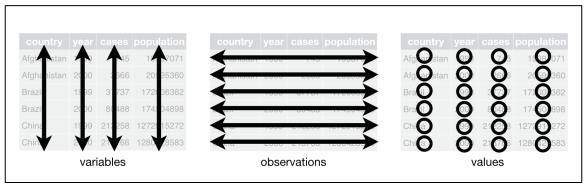
\includegraphics[width=8.14in]{tidy} 

}

\caption{Visualisasi 3 rule tidy data}\label{fig:tidy}
\end{figure}

Pada dataset \texttt{storms} terdapat 4 buah kolom dan 6 buah baris.
Masing-masing kolom menyatakan variabel pada masing-masing observasi
seperti nama badai , kecepatan angin, tekanan dan waktu . Ketiga syarat
kerapihan data sudah terpenuhi pada data tersebut sehingga kita bisa
melakukan analisa terhadap data tersebut, misalnya kecepatan angin dan
tekanan pada masing-masing badai. Selain itu kita juga dapat dengan
mudah menginput variabel baru pada dataset tersebut, misal: rasio
(kecepatan angin/tekanan).

Berikut adalah contoh bagaimana kita dapat dengan mudah menarik nilai
variabel pada masing-masing kolom dan membentuk variabel baru pada
dataset tersebut:

\begin{Shaded}
\begin{Highlighting}[]
\CommentTok{# subset variabel}
\NormalTok{storms}\OperatorTok{$}\NormalTok{storm}
\end{Highlighting}
\end{Shaded}

\begin{verbatim}
## [1] "Alberto" "Alex"    "Allison" "Ana"     "Arlene"  "Arthur"
\end{verbatim}

\begin{Shaded}
\begin{Highlighting}[]
\NormalTok{storms}\OperatorTok{$}\NormalTok{wind}
\end{Highlighting}
\end{Shaded}

\begin{verbatim}
## [1] 110  45  65  40  50  45
\end{verbatim}

\begin{Shaded}
\begin{Highlighting}[]
\NormalTok{storms}\OperatorTok{$}\NormalTok{pressure}
\end{Highlighting}
\end{Shaded}

\begin{verbatim}
## [1] 1007 1009 1005 1013 1010 1010
\end{verbatim}

\begin{Shaded}
\begin{Highlighting}[]
\NormalTok{storms}\OperatorTok{$}\NormalTok{date}
\end{Highlighting}
\end{Shaded}

\begin{verbatim}
## [1] "2000-08-03" "1998-07-27" "1995-06-03" "1997-06-30" "1999-06-11"
## [6] "1996-06-17"
\end{verbatim}

\begin{Shaded}
\begin{Highlighting}[]
\CommentTok{# membuat variabel baru}
\NormalTok{storms_new <-}\StringTok{ }\NormalTok{storms}
\NormalTok{storms_new}\OperatorTok{$}\NormalTok{ratio <-}\StringTok{ }\NormalTok{storms_new}\OperatorTok{$}\NormalTok{wind}\OperatorTok{/}\NormalTok{storms_new}\OperatorTok{$}\NormalTok{pressure}
\NormalTok{storms_new}
\end{Highlighting}
\end{Shaded}

\begin{verbatim}
##     storm wind pressure       date      ratio
## 1 Alberto  110     1007 2000-08-03 0.10923535
## 2    Alex   45     1009 1998-07-27 0.04459861
## 3 Allison   65     1005 1995-06-03 0.06467662
## 4     Ana   40     1013 1997-06-30 0.03948667
## 5  Arlene   50     1010 1999-06-11 0.04950495
## 6  Arthur   45     1010 1996-06-17 0.04455446
\end{verbatim}

Pada dataset \texttt{cases} terdapat 3 buah kolom dan 3 baris. Pada
kolom pertama berupa kode Negara, sedangkan kolom sisanya merupakan
tahun. Jika kita perhatikan dengan seksama dataset tersebut merupakan
sebuah \emph{contingency table} dimana tabel tersebut menyatakan
frekuensi kejadian pada tahun tertentu dan negara tertentu. Dataset
tersebut belum dapat dikatan \emph{tidy} karena kolom \texttt{2011}
sampai \texttt{2013} merupakan sebuah nilai dari observasi dan bukan
sebuah variabel sehingga dataset tersebut masih tergolong dataset
\emph{messy}. Selain itu sangat sulit untuk dilakukan penarikan terhadap
nilai pada setiap kolom serta pembentukan variabel baru sebagai
pendukung analisa juga sulit dilakukan. Berikut adalah contoh melakukan
penarikan nilai / subset pada masing variabel:

\begin{Shaded}
\begin{Highlighting}[]
\NormalTok{cases}\OperatorTok{$}\NormalTok{country}
\end{Highlighting}
\end{Shaded}

\begin{verbatim}
## [1] "FR" "DE" "US"
\end{verbatim}

\begin{Shaded}
\begin{Highlighting}[]
\KeywordTok{names}\NormalTok{(cases[}\OperatorTok{-}\DecValTok{1}\NormalTok{])}
\end{Highlighting}
\end{Shaded}

\begin{verbatim}
## [1] "2011" "2012" "2013"
\end{verbatim}

\begin{Shaded}
\begin{Highlighting}[]
\KeywordTok{unlist}\NormalTok{(cases[}\DecValTok{1}\OperatorTok{:}\DecValTok{3}\NormalTok{, }\DecValTok{2}\OperatorTok{:}\DecValTok{4}\NormalTok{])}
\end{Highlighting}
\end{Shaded}

\begin{verbatim}
## 20111 20112 20113 20121 20122 20123 20131 20132 20133 
##  7000  5800 15000  6900  6000 14000  7000  6200 13000
\end{verbatim}

Pada dataset \texttt{pollution}terdapat 3 buah kolom dan 6 baris.
Masing-masing kolom menyatakan lokasi berupa nama kota, keterangan
ukuran partikel, serta nilai dari ukuran partikel. Beberapa dari kita
mungkin menganggap dataset ini telah memenuhi syarat kerapihan data.
Namun, coba kita cermati jika mita ingin membuat variabel baru terkait
dengan berapa rentang ukuran partikel (range ukuran partikel) pada
masing-masing kota. Hal tersebut tentu sangat sulit dilakukan pada
dataset tersebut, namun dataset tersebut memungkinkan kita dengan mudah
mengambil nilai dari masing-masing variabelnya seperti contoh berikut:

\begin{Shaded}
\begin{Highlighting}[]
\NormalTok{pollution}\OperatorTok{$}\NormalTok{city}
\end{Highlighting}
\end{Shaded}

\begin{verbatim}
## [1] "New York" "New York" "London"   "London"   "Beijing"  "Beijing"
\end{verbatim}

\begin{Shaded}
\begin{Highlighting}[]
\NormalTok{pollution}\OperatorTok{$}\NormalTok{size}
\end{Highlighting}
\end{Shaded}

\begin{verbatim}
## [1] "large" "small" "large" "small" "large" "small"
\end{verbatim}

\begin{Shaded}
\begin{Highlighting}[]
\NormalTok{pollution}\OperatorTok{$}\NormalTok{amount}
\end{Highlighting}
\end{Shaded}

\begin{verbatim}
## [1]  23  14  22  16 121  56
\end{verbatim}

Berdasarkan contoh-contoh tersebut pada pembahasan kali ini penulis akan
menjelaskan bagaiman cara melakukan perapihan data menggunakan library
\texttt{tidyr}. Sebelum kita melakukannya berikut adalah sintaks untuk
menginstall library tersebut:

\begin{Shaded}
\begin{Highlighting}[]
\CommentTok{# memasang paket}
\KeywordTok{install.packages}\NormalTok{(}\StringTok{"tidyr"}\NormalTok{)}
\end{Highlighting}
\end{Shaded}

\begin{Shaded}
\begin{Highlighting}[]
\CommentTok{# memuat paket}
\KeywordTok{library}\NormalTok{(tidyr)}
\end{Highlighting}
\end{Shaded}

\subsection{Gather}\label{gather}

Pada dataset \texttt{cases} kolom \texttt{2011} sampai \texttt{2013}
perlu dijadikan satu variabel yaitu tahun. untuk melakukannya kita dapat
menggunakan fungsi \texttt{gather()}. Secara sederhana fungsi tersebut
dapat dituliskan dengan format sebagai berikut:

\begin{Shaded}
\begin{Highlighting}[]
\KeywordTok{gather}\NormalTok{(data, key, value, ...)}
\end{Highlighting}
\end{Shaded}

\begin{quote}
\textbf{Note: }

\begin{itemize}
\tightlist
\item
  \textbf{data}: data frame
\item
  \textbf{key, value}: nama kunci dan kolom nilai yang akan dibuat di
  output
\item
  \textbf{\ldots{}}: Spesifikasi kolom untuk dikumpulkan. Nilai yang
  diizinkan adalah:

  \begin{itemize}
  \tightlist
  \item
    nama variabel
  \item
    jika kita ingin memilih semua variabel antara a dan e, gunakan a:e
  \item
    jika kita ingin mengecualikan nama kolom y gunakan -y
  \item
    untuk opsi lainnya, lihat: \texttt{dplyr::select()}
  \end{itemize}
\end{itemize}
\end{quote}

Berikut adalah contoh penerapannya pada dataset \texttt{cases}:

\begin{Shaded}
\begin{Highlighting}[]
\CommentTok{# Ubah dataset cases menjadi tibble simpan sebagai objek cases_new}
\KeywordTok{library}\NormalTok{(tibble)}
\NormalTok{cases_tbl <-}\StringTok{ }\KeywordTok{as_tibble}\NormalTok{(cases)}

\CommentTok{# print}
\NormalTok{cases_tbl}
\end{Highlighting}
\end{Shaded}

\begin{verbatim}
## # A tibble: 3 x 4
##   country `2011` `2012` `2013`
##   <chr>    <dbl>  <dbl>  <dbl>
## 1 FR        7000   6900   7000
## 2 DE        5800   6000   6200
## 3 US       15000  14000  13000
\end{verbatim}

\begin{Shaded}
\begin{Highlighting}[]
\CommentTok{# gather}
\NormalTok{cases_new <-}\StringTok{ }\KeywordTok{gather}\NormalTok{(cases_tbl, }
                    \CommentTok{# variabel kunci}
                    \DataTypeTok{key =} \StringTok{"year"}\NormalTok{,}
                    \CommentTok{# nilai variabel}
                    \DataTypeTok{value =} \StringTok{"frequency"}\NormalTok{,}
                    \CommentTok{# kecualikan kolom country}
                    \OperatorTok{-}\NormalTok{country)}

\CommentTok{# print}
\NormalTok{cases_new}
\end{Highlighting}
\end{Shaded}

\begin{verbatim}
## # A tibble: 9 x 3
##   country year  frequency
##   <chr>   <chr>     <dbl>
## 1 FR      2011       7000
## 2 DE      2011       5800
## 3 US      2011      15000
## 4 FR      2012       6900
## 5 DE      2012       6000
## 6 US      2012      14000
## 7 FR      2013       7000
## 8 DE      2013       6200
## 9 US      2013      13000
\end{verbatim}

Berdasarkan hasil yang diperoleh terlihat bahwa variabel tahun memiliki
jenis data karakter. Jenis data ini masih belum sesuai sehingga perlu
dikonversi agar menjadi jenis data numerik (\emph{dbl = double}). Untuk
melakukannya jalankan sintaks berikut:

\begin{Shaded}
\begin{Highlighting}[]
\CommentTok{# Ubah jenis variabel tahun menjadi numerik}
\NormalTok{cases_new}\OperatorTok{$}\NormalTok{year <-}\StringTok{ }\KeywordTok{as.numeric}\NormalTok{(cases_new}\OperatorTok{$}\NormalTok{year)}
\NormalTok{cases_new}
\end{Highlighting}
\end{Shaded}

\begin{verbatim}
## # A tibble: 9 x 3
##   country  year frequency
##   <chr>   <dbl>     <dbl>
## 1 FR       2011      7000
## 2 DE       2011      5800
## 3 US       2011     15000
## 4 FR       2012      6900
## 5 DE       2012      6000
## 6 US       2012     14000
## 7 FR       2013      7000
## 8 DE       2013      6200
## 9 US       2013     13000
\end{verbatim}

Data yang diperoleh sekaran telah rapi (\emph{tidy}), sehingga sudah
siap untuk dilakukan analisa data.

\subsection{Spread}\label{spread}

Fungsi \texttt{spread()} berkebalikan dengan \texttt{gather()}. Fungsi
\texttt{gather()} menggabungkan beberapa kolom menjadi 2 buah kolom
kolom kunci sedangkan \texttt{spread()} merubah dua kolom menjadi
beberapa kolom. Format sederhanya adalah sebagai berikut:

\begin{quote}
\textbf{Note: }

\begin{itemize}
\tightlist
\item
  \textbf{data}: data frame
\item
  \textbf{key}: nama kolom yang akan dijadikan heading pada kolom baru
\item
  \textbf{value}: nama kolom yang nilainya akan mengisi setiap sel
\end{itemize}
\end{quote}

Pada contoh kasus pada data \texttt{pollution}, kita dapat memisahkan
kolom 2 menjadi kolom baru yaitu kolom \texttt{big\ size} dan
\texttt{small\ size}. Untuk melakukannya jalankan sintaks berikut:

\begin{Shaded}
\begin{Highlighting}[]
\CommentTok{# merubah objek pollution menjadi tibble}
\NormalTok{pollution_tbl <-}\StringTok{ }\KeywordTok{as_tibble}\NormalTok{(pollution)}

\CommentTok{# print}
\NormalTok{pollution_tbl}
\end{Highlighting}
\end{Shaded}

\begin{verbatim}
## # A tibble: 6 x 3
##   city     size  amount
##   <chr>    <chr>  <dbl>
## 1 New York large     23
## 2 New York small     14
## 3 London   large     22
## 4 London   small     16
## 5 Beijing  large    121
## 6 Beijing  small     56
\end{verbatim}

\begin{Shaded}
\begin{Highlighting}[]
\CommentTok{# spread}
\NormalTok{pollution_new <-}\StringTok{ }\KeywordTok{spread}\NormalTok{(pollution_tbl,}
                        \DataTypeTok{key =}\NormalTok{ size,}
                        \DataTypeTok{value =}\NormalTok{ amount)}

\CommentTok{#print}
\NormalTok{pollution_new}
\end{Highlighting}
\end{Shaded}

\begin{verbatim}
## # A tibble: 3 x 3
##   city     large small
##   <chr>    <dbl> <dbl>
## 1 Beijing    121    56
## 2 London      22    16
## 3 New York    23    14
\end{verbatim}

Terlihat bahwa data \texttt{pollution} tampak memnuhi syarat kerapihan
data (\emph{tidy}). Kita sekarang dapat menginput variabel baru dan
melakukan analisa terhadap data tersebut. Berikut adalah contoh
penerapannya:

\begin{Shaded}
\begin{Highlighting}[]
\CommentTok{# input variabel range (large-small)}
\NormalTok{pollution_new}\OperatorTok{$}\NormalTok{range <-}\StringTok{ }\NormalTok{pollution_new}\OperatorTok{$}\NormalTok{large }\OperatorTok{-}\StringTok{ }\NormalTok{pollution_new}\OperatorTok{$}\NormalTok{small}

\CommentTok{# print}
\NormalTok{pollution_new}
\end{Highlighting}
\end{Shaded}

\begin{verbatim}
## # A tibble: 3 x 4
##   city     large small range
##   <chr>    <dbl> <dbl> <dbl>
## 1 Beijing    121    56    65
## 2 London      22    16     6
## 3 New York    23    14     9
\end{verbatim}

Berdasarkan hasil yang diperoleh diketahui bahwa nilai range ukuran
partikel terbesar berada di Kota Beijing.

\subsection{Separate}\label{separate}

Fungsi \texttt{separate()} merupakan fungsi yang digunakan untuk
memisahkan sejumlah nilai pada sebuah kolom menjadi beberapa kolom
berdasarkan karakter pemisah yang ada di dalam nilai suatu kolom. Fungsi
ini berbeda dengan fungsi sebelumnya seperti \texttt{gather()} dan
\texttt{spread()} yang menggabung atau memisahkan 2 atau beberapa kolom.
Format sederhana fungsi \texttt{separate()} adalah sebagai berikut:

\begin{Shaded}
\begin{Highlighting}[]
\KeywordTok{separate}\NormalTok{(data, col, into, }\DataTypeTok{sep =} \StringTok{"[^[:alnum:]]+"}\NormalTok{, }\DataTypeTok{convert=} \OtherTok{TRUE}\NormalTok{)}
\end{Highlighting}
\end{Shaded}

\begin{quote}
\textbf{Note: }

\begin{itemize}
\tightlist
\item
  \textbf{data}: data frame.
\item
  \textbf{col}: Nama kolom yang tidak dikutip.
\item
  \textbf{into}: Vektor karakter menentukan nama variabel baru yang akan
  dibuat.
\item
  \textbf{sep}: Pemisah antar kolom:
\item
  Jika karakter, diartikan sebagai ekspresi reguler. Jika numerik,
  diartikan sebagai posisi untuk dibelah. Nilai-nilai positif mulai dari
  1 di ujung kiri string; nilai negatif mulai dari -1 di ujung kanan
  string.
\item
  \textbf{convert}: nilai logik. Jika bernilai TRUE maka kolom baru yang
  akan diperoleh akan dikonversi berdasarkan jenis data yang seharusnya.
\end{itemize}
\end{quote}

Pada dataset \texttt{storms} kita ingin memisahkan kolom \texttt{date}
menjadi beberapa kolom seperti \texttt{year}, \texttt{month}, dan
\texttt{day}, Kita dapat menggunakan fungsi \texttt{separate()} untuk
memisahkan nilai pada kolom tersebut berdasarkan karakter pemisah pada
nilai kolom tersebut dalam hal ini adalah ``-''. Berikut adalah cara
melakukannya:

\begin{Shaded}
\begin{Highlighting}[]
\CommentTok{# merubah storms menjadi tibble}
\NormalTok{storms_tbl <-}\StringTok{ }\KeywordTok{as_tibble}\NormalTok{(storms)}

\CommentTok{# print}
\NormalTok{storms_tbl}
\end{Highlighting}
\end{Shaded}

\begin{verbatim}
## # A tibble: 6 x 4
##   storm    wind pressure date      
##   <chr>   <int>    <int> <date>    
## 1 Alberto   110     1007 2000-08-03
## 2 Alex       45     1009 1998-07-27
## 3 Allison    65     1005 1995-06-03
## 4 Ana        40     1013 1997-06-30
## 5 Arlene     50     1010 1999-06-11
## 6 Arthur     45     1010 1996-06-17
\end{verbatim}

\begin{Shaded}
\begin{Highlighting}[]
\CommentTok{# separate}
\NormalTok{storms_new <-}\StringTok{ }\KeywordTok{separate}\NormalTok{(storms_tbl,}
                       \DataTypeTok{col =}\NormalTok{ date,}
                       \DataTypeTok{into =} \KeywordTok{c}\NormalTok{(}\StringTok{"year"}\NormalTok{,}\StringTok{"month"}\NormalTok{,}\StringTok{"days"}\NormalTok{),}
                       \DataTypeTok{sep =} \StringTok{"-"}\NormalTok{,}
                       \DataTypeTok{convert =} \OtherTok{TRUE}\NormalTok{)}

\CommentTok{# print}
\NormalTok{storms_new}
\end{Highlighting}
\end{Shaded}

\begin{verbatim}
## # A tibble: 6 x 6
##   storm    wind pressure  year month  days
##   <chr>   <int>    <int> <int> <int> <int>
## 1 Alberto   110     1007  2000     8     3
## 2 Alex       45     1009  1998     7    27
## 3 Allison    65     1005  1995     6     3
## 4 Ana        40     1013  1997     6    30
## 5 Arlene     50     1010  1999     6    11
## 6 Arthur     45     1010  1996     6    17
\end{verbatim}

Berdasarkan hasil yang diperoleh terlihat bahwa data telah terpisah
dengan benar yang ditunjukkan dari nilai yang terpisah dan jenis data
yang dihasilkan.

\subsection{Unite}\label{unite}

Fungsi \texttt{unite()} merupakan kebalikan dari fungsi
\texttt{separate()}, dimana fungsi ini menggabungkan sejumlah kolom
menjadi 1 kolom. Format sederhana untuk melakukanya disajikan sebagai
berikut:

\begin{Shaded}
\begin{Highlighting}[]
\KeywordTok{unite}\NormalTok{(data, col, ..., }\DataTypeTok{sep =} \StringTok{"_"}\NormalTok{)}
\end{Highlighting}
\end{Shaded}

\begin{quote}
\textbf{Note: }

\begin{itemize}
\tightlist
\item
  \textbf{data}: data frame.
\item
  \textbf{col}: nama kolom baru (tanpa tanda kutip) untuk ditambahkan.
\item
  \textbf{sep}: pemisah yang akan digunakan pada antar nilai.
\end{itemize}
\end{quote}

Pada dataset \texttt{storms\_new} kita ingin menggabungkan kembali kolom
\texttt{year}, \texttt{month}, dan \texttt{days} dengan karakter pemisah
``/''. Berikut adalah cara melakukannya:

\begin{Shaded}
\begin{Highlighting}[]
\CommentTok{# unite}
\NormalTok{storms_old <-}\StringTok{ }\KeywordTok{unite}\NormalTok{(storms_new,}
                   \DataTypeTok{col =} \StringTok{"date"}\NormalTok{,}
\NormalTok{                   year, month, days,}
                   \DataTypeTok{sep =} \StringTok{"-"}\NormalTok{)}

\CommentTok{# print}
\NormalTok{storms_old}
\end{Highlighting}
\end{Shaded}

\begin{verbatim}
## # A tibble: 6 x 4
##   storm    wind pressure date     
##   <chr>   <int>    <int> <chr>    
## 1 Alberto   110     1007 2000-8-3 
## 2 Alex       45     1009 1998-7-27
## 3 Allison    65     1005 1995-6-3 
## 4 Ana        40     1013 1997-6-30
## 5 Arlene     50     1010 1999-6-11
## 6 Arthur     45     1010 1996-6-17
\end{verbatim}

\begin{Shaded}
\begin{Highlighting}[]
\CommentTok{# ubah jenis kolom menjadi date}
\NormalTok{storms_old}\OperatorTok{$}\NormalTok{date <-}\StringTok{ }\KeywordTok{as.Date}\NormalTok{(storms_old}\OperatorTok{$}\NormalTok{date)}

\CommentTok{# print}
\NormalTok{storms_old}
\end{Highlighting}
\end{Shaded}

\begin{verbatim}
## # A tibble: 6 x 4
##   storm    wind pressure date      
##   <chr>   <int>    <int> <date>    
## 1 Alberto   110     1007 2000-08-03
## 2 Alex       45     1009 1998-07-27
## 3 Allison    65     1005 1995-06-03
## 4 Ana        40     1013 1997-06-30
## 5 Arlene     50     1010 1999-06-11
## 6 Arthur     45     1010 1996-06-17
\end{verbatim}

\section{Transformasi Data}\label{transformasi-data}

Data frame merupakan struktur data utama dalam statistik dan dalam
\texttt{R}. Struktur dasar data frame ialah ada satu observasi tiap
baris dan setiap kolom mewakili variabel, ukuran, fitur, atau
karakteristik pengamatan itu yang telah dijelaskan pada bagian
sebelumya. \texttt{R} memiliki implementasi internal data frame yang
kemungkinan besar akan kita gunakan paling sering. Namun, ada paket di
CRAN yang mengimplementasikan data frame layaknya basis data relasional
yang memungkinkan kita untuk beroperasi pada data frame yang sangat
besar.

Mengingat pentingnya mengelola dat frame, penting bagi kita untuk
memiliki alat yang baik untuk melakukannya. \texttt{R} memiliki beberapa
paket seperti fungsi \texttt{subset()} dan penggunaan operator ``{[}''
dan ``\$'' untuk mengekstrak himpunan bagian dari frame data. Namun,
operasi lain, seperti pemfilteran, pengurutan, dan pengelompokan data,
seringkali dapat menjadi operasi yang membosankan di \texttt{R} yang
sintaksisnya tidak terlalu intuitif. Paket \texttt{dplyr} dirancang
untuk mengurangi banyak masalah ini dan menyediakan serangkaian
rutinitas yang dioptimalkan secara khusus untuk menangani data frame.

\subsection{Paket dplyr}\label{paket-dplyr}

Paket \texttt{dplyr} dikembangkan oleh \textbf{Hadley Wickham} dari
\textbf{RStudio} dan merupakan versi yang dioptimalkan dari paket
\texttt{plyr}-nya. Paket \texttt{dplyr} tidak menyediakan fungsionalitas
baru untuk \texttt{R} sendiri, dalam arti bahwa semua yang dilakukan
\texttt{dplyr} sudah dapat dilakukan dengan fungsi basis \texttt{R},
tetapi sangat menyederhanakan fungsi yang ada di \texttt{R}.

Salah satu kontribusi penting dari paket \texttt{dplyr} adalah ia
menyediakan ``\emph{grammar}'' (khususnya, kata kerja) untuk manipulasi
data dan untuk beroperasi pada data frame. Melalui \emph{grammar} ini,
kita dapat berkomunikasi dengan masuk akal apa yang telah kita lakukan
terhadap data frame dapat pula dipahami orang lain (dengan asumsi mereka
juga tahu \emph{grammar}-nya). Hal ini berguna karena memberikan
abstraksi untuk manipulasi data yang sebelumnya tidak ada. Kontribusi
lain yang bermanfaat adalah bahwa fungsi \texttt{dplyr} sangat cepat,
karena banyak operasi utama dikodekan dalam C++.

Pada bagian ini pembaca akan belajar \textbf{6} fungsi utama yang ada
pada paket \texttt{dplyr}. Fungsi tersebut antara lain:

\begin{enumerate}
\def\labelenumi{\arabic{enumi}.}
\tightlist
\item
  Mengambil sejumlah observasi berdasarkan nilainya (\texttt{filter()}).
\item
  Mengurutkan kembali baris data frame berdasarkan nilai pada sebuah
  atau beberapa variabel (\texttt{arrange()}).
\item
  Mengambil atau subset terhadap sebuah atau beberapa variabel
  berdasarkan nama variabel/kolom (\texttt{select()}).
\item
  Membuat variabel baru atau menambahkan kolom baru (\texttt{mutate()}).
\item
  Membuat ringkasan terhadap data frame (\texttt{summarize()})
\item
  Mengelompokkan operasi berdasarkan grup data (\texttt{group\_by()}).
\end{enumerate}

Keseluruhan fungsi tersebut format fungsi yang seragam, yaitu:

\begin{enumerate}
\def\labelenumi{\arabic{enumi}.}
\tightlist
\item
  Argumen pertama adalah data frame.
\item
  Argumen selanjutnya adalah deskripsi yang akan dilakukan terhadap data
  frame (filter, pengurutan kembali, membuat ringkasan, dll) menggunakan
  nama variabel (tanpa tanda kutip).
\item
  Hasil operasi yang diperoleh adalah data frame baru.
\end{enumerate}

Untuk menginstall dan memuat paket \texttt{dplyr} jalankan sintaks
berikut:

\begin{Shaded}
\begin{Highlighting}[]
\CommentTok{# Memasang paket}
\KeywordTok{install.packages}\NormalTok{(}\StringTok{"dplyr"}\NormalTok{)}
\end{Highlighting}
\end{Shaded}

\begin{Shaded}
\begin{Highlighting}[]
\CommentTok{# memuat paket}
\KeywordTok{library}\NormalTok{(dplyr)}
\end{Highlighting}
\end{Shaded}

\subsection{filter()}\label{filter}

Fungsi \texttt{filter()} digunakan untuk mengekstrak himpunan bagian
(subset) baris dari data frame. Fungsi ini mirip dengan fungsi
\texttt{subset()} yang ada di \texttt{R}. Secara sederhana format fungsi
\texttt{filter()} dapat dituliskan sebagai berikut:

\begin{Shaded}
\begin{Highlighting}[]
\KeywordTok{filter}\NormalTok{(data, ....)}
\end{Highlighting}
\end{Shaded}

\begin{quote}
\textbf{Note: }

\begin{itemize}
\tightlist
\item
  \textbf{data} : data frame
\item
  \textbf{\ldots{}.} : Predikat logis didefinisikan dalam istilah
  variabel dalam \textbf{data}. Beberapa kondisi digabungkan dengan \&
  (lihat Chapter 2 opeator relasi dan operator logika. Hanya baris
  tempat kondisi bernilai TRUE disimpan.
\end{itemize}
\end{quote}

Misalkan kita akan melakukan melakukan filter terhadap data frame
\texttt{pollution\_tbl} terhadap variabel \texttt{size} dengan kriteria
\texttt{large} dan \texttt{amount} \textgreater{} 12. Berikut adalah
sintaks yang digunakan:

\begin{Shaded}
\begin{Highlighting}[]
\KeywordTok{filter}\NormalTok{(pollution_tbl, size}\OperatorTok{==}\StringTok{"large"} \OperatorTok{&}\StringTok{ }\NormalTok{amount }\OperatorTok{>}\StringTok{ }\DecValTok{12}\NormalTok{)}
\end{Highlighting}
\end{Shaded}

\begin{verbatim}
## # A tibble: 3 x 3
##   city     size  amount
##   <chr>    <chr>  <dbl>
## 1 New York large     23
## 2 London   large     22
## 3 Beijing  large    121
\end{verbatim}

Jika menggunakan paket dasar \texttt{R}:

\begin{Shaded}
\begin{Highlighting}[]
\KeywordTok{subset}\NormalTok{(pollution_tbl,size}\OperatorTok{==}\StringTok{"large"} \OperatorTok{&}\StringTok{ }\NormalTok{amount }\OperatorTok{>}\StringTok{ }\DecValTok{12}\NormalTok{)}
\end{Highlighting}
\end{Shaded}

\begin{verbatim}
## # A tibble: 3 x 3
##   city     size  amount
##   <chr>    <chr>  <dbl>
## 1 New York large     23
## 2 London   large     22
## 3 Beijing  large    121
\end{verbatim}

Operator ``\textgreater{}'' merupakan operator relasi (lihat chapter 2:
operator relasi). Operator tersebut banyak digunakan untuk melakukan
filter terhadap variabel/kolom yang mengandung nilai numerik.

Operator ``=='' merupakan operator logika (lihat chapter 2: operator
logika). Operator tersebut digunakan untuk melakukan filter terhadap
sejumlah syarat atau kondisi yang kita tetapkan. Jika nilai yang
dihasilkan TRUE, maka hanya observasi tersebut yang akan ditampilkan.
Untuk lebih memahami penerapan masing-masing operator logika pada proses
filter perhatikan Figure \ref{fig:filter} berikut:

\begin{figure}

{\centering 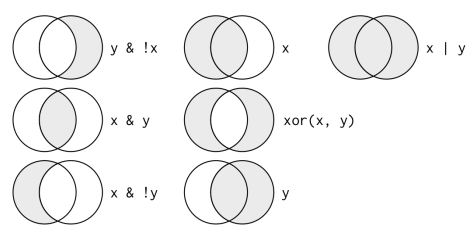
\includegraphics[width=6.57in]{filter} 

}

\caption{Diagram operasi Boolean}\label{fig:filter}
\end{figure}

\begin{quote}
\textbf{Note: } Bagian yang di arsir adalah observasi yang akan
ditampilkan pada output.
\end{quote}

Salah satu bagian terpenting dan paling sering penulis gunakan pada
fungsi ini memfilter \emph{missing value} (melihat observasi yang
mengandung \emph{missing value} atau tidak melibatkan \emph{missing
value}). Berikut adalah contoh filter terhadap data pada
\texttt{pollution\_tbl} yang tidak mengandung \emph{missing value} dan
nilai \texttt{amount}\textgreater{}0.

\begin{Shaded}
\begin{Highlighting}[]
\KeywordTok{filter}\NormalTok{(pollution_tbl,}\OperatorTok{!}\NormalTok{(}\KeywordTok{is.na}\NormalTok{(amount)}\OperatorTok{|}\NormalTok{amount}\OperatorTok{<=}\DecValTok{0}\NormalTok{))}
\end{Highlighting}
\end{Shaded}

\begin{verbatim}
## # A tibble: 6 x 3
##   city     size  amount
##   <chr>    <chr>  <dbl>
## 1 New York large     23
## 2 New York small     14
## 3 London   large     22
## 4 London   small     16
## 5 Beijing  large    121
## 6 Beijing  small     56
\end{verbatim}

Berdasarkan hasil yang diperoleh seluruh data tidak ada yang di drop
sehingga dapat disimpulkan bahwa data tersebut tidak mengandung
\emph{missing value} dan nol.

\subsection{arrange()}\label{arrange}

Fungsi \texttt{arrange()} bekerja mirip dengan fungsi \texttt{filter()}
kecuali bahwa alih-alih memilih baris, fungsi ini mengubah urutan
observasinya (mengurutkan dari yang terbesar atau sebaliknya).
Dibutuhkan data frame dan sekumpulan nama kolom (atau ekspresi yang
lebih rumit) untuk dipesan. Jika kita memberikan lebih dari satu nama
kolom pada fungsi, setiap kolom tambahan akan digunakan untuk menentukan
urutan nilai yang sama berdasarkan nilai kolom sebelumnya.

Fungsi \texttt{arrange()} mirip dengan fungsi \texttt{order()} pada
paket dasar \texttt{R}. Format sederhana fungsi ini adalah sebagai
berikut:

\begin{Shaded}
\begin{Highlighting}[]
\KeywordTok{arrange}\NormalTok{(data, ....)}
\end{Highlighting}
\end{Shaded}

\begin{quote}
\textbf{Note: }

\begin{itemize}
\tightlist
\item
  \textbf{data} : data frame
\item
  \textbf{\ldots{}.} : daftar nama variabel yang tidak dikutip yang
  dipisahkan tanda koma, atau ekspresi yang melibatkan nama variabel.
  Gunakan \texttt{desc()} untuk mengurutkan variabel dalam urutan
  menurun.
\end{itemize}
\end{quote}

Misalkan kita ingin melihat urutan mobil pada data \texttt{mtcars}
berdasarkan penggunaan bahan bakar (\texttt{mpg}) dan bobot mobil
(\texttt{wt}) tersebut. Berikut adalah sintaks yang digunakan:

\begin{Shaded}
\begin{Highlighting}[]
\KeywordTok{data}\NormalTok{(}\StringTok{"mtcars"}\NormalTok{)}

\CommentTok{# Ubah mtcars menjadi tibble}
\NormalTok{mtcars<-}\StringTok{ }\KeywordTok{as_tibble}\NormalTok{(mtcars)}

\KeywordTok{arrange}\NormalTok{(mtcars, mpg, wt)}
\end{Highlighting}
\end{Shaded}

\begin{verbatim}
## # A tibble: 32 x 11
##      mpg   cyl  disp    hp  drat    wt  qsec    vs    am  gear  carb
##    <dbl> <dbl> <dbl> <dbl> <dbl> <dbl> <dbl> <dbl> <dbl> <dbl> <dbl>
##  1  10.4     8  472    205  2.93  5.25  18.0     0     0     3     4
##  2  10.4     8  460    215  3     5.42  17.8     0     0     3     4
##  3  13.3     8  350    245  3.73  3.84  15.4     0     0     3     4
##  4  14.3     8  360    245  3.21  3.57  15.8     0     0     3     4
##  5  14.7     8  440    230  3.23  5.34  17.4     0     0     3     4
##  6  15       8  301    335  3.54  3.57  14.6     0     1     5     8
##  7  15.2     8  304    150  3.15  3.44  17.3     0     0     3     2
##  8  15.2     8  276.   180  3.07  3.78  18       0     0     3     3
##  9  15.5     8  318    150  2.76  3.52  16.9     0     0     3     2
## 10  15.8     8  351    264  4.22  3.17  14.5     0     1     5     4
## # ... with 22 more rows
\end{verbatim}

Jika ingin urutan yang digunakan adalah dari yang terbesar ke terkecil
untuk kedua variabel tersebut jalankan sintaks berikut:

\begin{Shaded}
\begin{Highlighting}[]
\KeywordTok{arrange}\NormalTok{(mtcars, }\KeywordTok{desc}\NormalTok{(mpg), }\KeywordTok{desc}\NormalTok{(wt))}
\end{Highlighting}
\end{Shaded}

\begin{verbatim}
## # A tibble: 32 x 11
##      mpg   cyl  disp    hp  drat    wt  qsec    vs    am  gear  carb
##    <dbl> <dbl> <dbl> <dbl> <dbl> <dbl> <dbl> <dbl> <dbl> <dbl> <dbl>
##  1  33.9     4  71.1    65  4.22  1.84  19.9     1     1     4     1
##  2  32.4     4  78.7    66  4.08  2.2   19.5     1     1     4     1
##  3  30.4     4  75.7    52  4.93  1.62  18.5     1     1     4     2
##  4  30.4     4  95.1   113  3.77  1.51  16.9     1     1     5     2
##  5  27.3     4  79      66  4.08  1.94  18.9     1     1     4     1
##  6  26       4 120.     91  4.43  2.14  16.7     0     1     5     2
##  7  24.4     4 147.     62  3.69  3.19  20       1     0     4     2
##  8  22.8     4 141.     95  3.92  3.15  22.9     1     0     4     2
##  9  22.8     4 108      93  3.85  2.32  18.6     1     1     4     1
## 10  21.5     4 120.     97  3.7   2.46  20.0     1     0     3     1
## # ... with 22 more rows
\end{verbatim}

Jika menggunakan fungsi \texttt{order()}:

\begin{Shaded}
\begin{Highlighting}[]
\KeywordTok{attach}\NormalTok{(mtcars)}
\CommentTok{# urutan dari kecil ke besar}
\NormalTok{mtcars[}\KeywordTok{order}\NormalTok{(mpg, wt), ]}
\end{Highlighting}
\end{Shaded}

\begin{verbatim}
## # A tibble: 32 x 11
##      mpg   cyl  disp    hp  drat    wt  qsec    vs    am  gear  carb
##    <dbl> <dbl> <dbl> <dbl> <dbl> <dbl> <dbl> <dbl> <dbl> <dbl> <dbl>
##  1  10.4     8  472    205  2.93  5.25  18.0     0     0     3     4
##  2  10.4     8  460    215  3     5.42  17.8     0     0     3     4
##  3  13.3     8  350    245  3.73  3.84  15.4     0     0     3     4
##  4  14.3     8  360    245  3.21  3.57  15.8     0     0     3     4
##  5  14.7     8  440    230  3.23  5.34  17.4     0     0     3     4
##  6  15       8  301    335  3.54  3.57  14.6     0     1     5     8
##  7  15.2     8  304    150  3.15  3.44  17.3     0     0     3     2
##  8  15.2     8  276.   180  3.07  3.78  18       0     0     3     3
##  9  15.5     8  318    150  2.76  3.52  16.9     0     0     3     2
## 10  15.8     8  351    264  4.22  3.17  14.5     0     1     5     4
## # ... with 22 more rows
\end{verbatim}

\begin{Shaded}
\begin{Highlighting}[]
\CommentTok{# urutan dari besar ke kecil}
\NormalTok{mtcars[}\KeywordTok{order}\NormalTok{(}\OperatorTok{-}\NormalTok{mpg, }\OperatorTok{-}\NormalTok{wt), ]}
\end{Highlighting}
\end{Shaded}

\begin{verbatim}
## # A tibble: 32 x 11
##      mpg   cyl  disp    hp  drat    wt  qsec    vs    am  gear  carb
##    <dbl> <dbl> <dbl> <dbl> <dbl> <dbl> <dbl> <dbl> <dbl> <dbl> <dbl>
##  1  33.9     4  71.1    65  4.22  1.84  19.9     1     1     4     1
##  2  32.4     4  78.7    66  4.08  2.2   19.5     1     1     4     1
##  3  30.4     4  75.7    52  4.93  1.62  18.5     1     1     4     2
##  4  30.4     4  95.1   113  3.77  1.51  16.9     1     1     5     2
##  5  27.3     4  79      66  4.08  1.94  18.9     1     1     4     1
##  6  26       4 120.     91  4.43  2.14  16.7     0     1     5     2
##  7  24.4     4 147.     62  3.69  3.19  20       1     0     4     2
##  8  22.8     4 141.     95  3.92  3.15  22.9     1     0     4     2
##  9  22.8     4 108      93  3.85  2.32  18.6     1     1     4     1
## 10  21.5     4 120.     97  3.7   2.46  20.0     1     0     3     1
## # ... with 22 more rows
\end{verbatim}

\begin{quote}
\textbf{Note: } \emph{missing value} akan selalu diurutkan pada
observasi terakhir baik menggunakan urutan dari terbesar ke terkecil
maupun sebaliknya.
\end{quote}

\subsection{select()}\label{select}

Fungsi \texttt{select()} dapat digunakan untuk memilih kolom dari data
frame yang ingin kita fokuskan. Seringkali kita memiliki data frame yang
besar yang berisi semua data, tetapi setiap analisis yang diberikan
hanya menggunakan subset variabel atau pengamatan. Fungsi
\texttt{select()} memungkinkan kita untuk mendapatkan beberapa kolom
yang mungkin kita butuhkan.

Fungsi \texttt{select()} memiliki kesamaan dengan subset menggunakan
tanda ``{[}'' dan ``\$''. Perbedaanya adalah kita dapat melakukan hal
lebih melalui fungsi ini seperti memilih berdasarkan kriteria tertentu
menggunakan fungsi bantuan sebagai berikut:

\begin{enumerate}
\def\labelenumi{\arabic{enumi}.}
\tightlist
\item
  \texttt{starts\_with("abcd")}, pilih kolom yang memiliki awalan
  ``abcd''.
\item
  \texttt{end\_with("abcd")}, pilih kolom yang memiliki akhiran
  ``abcd''.
\item
  \texttt{contains("abcd")}, pilih kolom yang mengandung nama ``abcd''
\item
  \texttt{matches("(.)\textbackslash{}\textbackslash{}1")}, pilih
  variabel yang mengandung \emph{regular expression}. Fungsi ini memilih
  variabel yang mengandung perulangan karakter.
\item
  \texttt{num\_range("x",\ 1:3)}, cocokkan berdasarkan kolom dengan nama
  x1,x2,x3.
\end{enumerate}

Berdasarkan fungsi bantuan tersebut, fungsi \texttt{select()} lebih
powerfull dibandingkan dengan cara subset biasa serta lebih mudah dalam
melakukannya. Berikut adalah format dari fungsi \texttt{select()}:

\begin{Shaded}
\begin{Highlighting}[]
\KeywordTok{select}\NormalTok{(data, ....)}
\end{Highlighting}
\end{Shaded}

\begin{quote}
\textbf{Note: }

\begin{itemize}
\tightlist
\item
  \textbf{data} : data frame
\item
  \textbf{\ldots{}.} : Satu atau lebih ekspresi kutip yang dipisahkan
  oleh koma. kita dapat memperlakukan nama variabel seperti posisi,
  sehingga kita dapat menggunakan ekspresi seperti x: y untuk memilih
  rentang variabel.Nilai positif pilih variabel; nilai negatif drop
  variabel. Jika ekspresi pertama negatif, \texttt{select()} akan secara
  otomatis dimulai dengan semua variabel. Gunakan argumen bernama, mis.
  \texttt{new\_name\ =\ old\_name}, untuk mengganti nama variabel yang
  dipilih.
\end{itemize}
\end{quote}

Berikut adalah contoh penerapan \texttt{selct()} pada data frame
\texttt{flights}.

\begin{Shaded}
\begin{Highlighting}[]
\CommentTok{# memasang paket}
\CommentTok{# install.packages("nycflights13")}

\CommentTok{# memuat data frame}
\KeywordTok{library}\NormalTok{(nycflights13)}

\CommentTok{# data}
\NormalTok{flights}
\end{Highlighting}
\end{Shaded}

\begin{verbatim}
## # A tibble: 336,776 x 19
##     year month   day dep_time sched_dep_time dep_delay arr_time
##    <int> <int> <int>    <int>          <int>     <dbl>    <int>
##  1  2013     1     1      517            515         2      830
##  2  2013     1     1      533            529         4      850
##  3  2013     1     1      542            540         2      923
##  4  2013     1     1      544            545        -1     1004
##  5  2013     1     1      554            600        -6      812
##  6  2013     1     1      554            558        -4      740
##  7  2013     1     1      555            600        -5      913
##  8  2013     1     1      557            600        -3      709
##  9  2013     1     1      557            600        -3      838
## 10  2013     1     1      558            600        -2      753
## # ... with 336,766 more rows, and 12 more variables: sched_arr_time <int>,
## #   arr_delay <dbl>, carrier <chr>, flight <int>, tailnum <chr>,
## #   origin <chr>, dest <chr>, air_time <dbl>, distance <dbl>, hour <dbl>,
## #   minute <dbl>, time_hour <dttm>
\end{verbatim}

\begin{Shaded}
\begin{Highlighting}[]
\CommentTok{# pilih kolom berdasarkan nama kolom}
\KeywordTok{select}\NormalTok{(flights, year, month, day)}
\end{Highlighting}
\end{Shaded}

\begin{verbatim}
## # A tibble: 336,776 x 3
##     year month   day
##    <int> <int> <int>
##  1  2013     1     1
##  2  2013     1     1
##  3  2013     1     1
##  4  2013     1     1
##  5  2013     1     1
##  6  2013     1     1
##  7  2013     1     1
##  8  2013     1     1
##  9  2013     1     1
## 10  2013     1     1
## # ... with 336,766 more rows
\end{verbatim}

\begin{Shaded}
\begin{Highlighting}[]
\CommentTok{# pilih seluruh kolom dari year sampai day}
\KeywordTok{select}\NormalTok{(flights, year}\OperatorTok{:}\NormalTok{day)}
\end{Highlighting}
\end{Shaded}

\begin{verbatim}
## # A tibble: 336,776 x 3
##     year month   day
##    <int> <int> <int>
##  1  2013     1     1
##  2  2013     1     1
##  3  2013     1     1
##  4  2013     1     1
##  5  2013     1     1
##  6  2013     1     1
##  7  2013     1     1
##  8  2013     1     1
##  9  2013     1     1
## 10  2013     1     1
## # ... with 336,766 more rows
\end{verbatim}

\begin{Shaded}
\begin{Highlighting}[]
\CommentTok{# drop kolom dari year sampai day}
\KeywordTok{select}\NormalTok{(flights, }\OperatorTok{-}\NormalTok{(year}\OperatorTok{:}\NormalTok{day))}
\end{Highlighting}
\end{Shaded}

\begin{verbatim}
## # A tibble: 336,776 x 16
##    dep_time sched_dep_time dep_delay arr_time sched_arr_time arr_delay
##       <int>          <int>     <dbl>    <int>          <int>     <dbl>
##  1      517            515         2      830            819        11
##  2      533            529         4      850            830        20
##  3      542            540         2      923            850        33
##  4      544            545        -1     1004           1022       -18
##  5      554            600        -6      812            837       -25
##  6      554            558        -4      740            728        12
##  7      555            600        -5      913            854        19
##  8      557            600        -3      709            723       -14
##  9      557            600        -3      838            846        -8
## 10      558            600        -2      753            745         8
## # ... with 336,766 more rows, and 10 more variables: carrier <chr>,
## #   flight <int>, tailnum <chr>, origin <chr>, dest <chr>, air_time <dbl>,
## #   distance <dbl>, hour <dbl>, minute <dbl>, time_hour <dttm>
\end{verbatim}

\begin{Shaded}
\begin{Highlighting}[]
\CommentTok{# pilih kolom dengan akhiran time}
\KeywordTok{select}\NormalTok{(flights, }\KeywordTok{ends_with}\NormalTok{(}\StringTok{"time"}\NormalTok{))}
\end{Highlighting}
\end{Shaded}

\begin{verbatim}
## # A tibble: 336,776 x 5
##    dep_time sched_dep_time arr_time sched_arr_time air_time
##       <int>          <int>    <int>          <int>    <dbl>
##  1      517            515      830            819      227
##  2      533            529      850            830      227
##  3      542            540      923            850      160
##  4      544            545     1004           1022      183
##  5      554            600      812            837      116
##  6      554            558      740            728      150
##  7      555            600      913            854      158
##  8      557            600      709            723       53
##  9      557            600      838            846      140
## 10      558            600      753            745      138
## # ... with 336,766 more rows
\end{verbatim}

\begin{Shaded}
\begin{Highlighting}[]
\CommentTok{# pilih kolom yang mengandung karakter "arr"}
\KeywordTok{select}\NormalTok{(flights, }\KeywordTok{contains}\NormalTok{(}\StringTok{"arr"}\NormalTok{))}
\end{Highlighting}
\end{Shaded}

\begin{verbatim}
## # A tibble: 336,776 x 4
##    arr_time sched_arr_time arr_delay carrier
##       <int>          <int>     <dbl> <chr>  
##  1      830            819        11 UA     
##  2      850            830        20 UA     
##  3      923            850        33 AA     
##  4     1004           1022       -18 B6     
##  5      812            837       -25 DL     
##  6      740            728        12 UA     
##  7      913            854        19 B6     
##  8      709            723       -14 EV     
##  9      838            846        -8 B6     
## 10      753            745         8 AA     
## # ... with 336,766 more rows
\end{verbatim}

Kita juga dapat menggunakan fungsi tambahan \texttt{everithing()} yang
berguna jika kita ingin memindahkan variabel yang menjadi fokus kita ke
awal data frame tanpa melakukan drop variabel. Berikut adalah contoh
sintaksnya:

\begin{Shaded}
\begin{Highlighting}[]
\CommentTok{# pindahkan kolom yang mengandung time di awal}
\KeywordTok{select}\NormalTok{(flights, }\KeywordTok{contains}\NormalTok{(}\StringTok{"time"}\NormalTok{), }\KeywordTok{everything}\NormalTok{())}
\end{Highlighting}
\end{Shaded}

\begin{verbatim}
## # A tibble: 336,776 x 19
##    dep_time sched_dep_time arr_time sched_arr_time air_time
##       <int>          <int>    <int>          <int>    <dbl>
##  1      517            515      830            819      227
##  2      533            529      850            830      227
##  3      542            540      923            850      160
##  4      544            545     1004           1022      183
##  5      554            600      812            837      116
##  6      554            558      740            728      150
##  7      555            600      913            854      158
##  8      557            600      709            723       53
##  9      557            600      838            846      140
## 10      558            600      753            745      138
## # ... with 336,766 more rows, and 14 more variables: time_hour <dttm>,
## #   year <int>, month <int>, day <int>, dep_delay <dbl>, arr_delay <dbl>,
## #   carrier <chr>, flight <int>, tailnum <chr>, origin <chr>, dest <chr>,
## #   distance <dbl>, hour <dbl>, minute <dbl>
\end{verbatim}

\subsection{mutate()}\label{mutate}

Fungsi \texttt{mutate()} ada untuk menghitung transformasi variabel
dalam data frame. Seringkali, kita ingin membuat variabel baru yang
berasal dari variabel yang ada dan fungsi \texttt{mutate()} menyediakan
antarmuka yang bersih untuk melakukan itu. Format yang digunakan adalah
sebagai berikut:

\begin{Shaded}
\begin{Highlighting}[]
\KeywordTok{mutate}\NormalTok{(data, ....)}
\end{Highlighting}
\end{Shaded}

\begin{quote}
\textbf{Note: }

\begin{itemize}
\tightlist
\item
  \textbf{data} : data frame
\item
  \textbf{\ldots{}.} : Pasangan nama-nilai ekspresi, masing-masing
  dengan panjang 1 atau panjang yang sama dengan jumlah baris dalam grup
  (jika menggunakan group\_by ()) atau di seluruh input (jika tidak
  menggunakan grup). Nama setiap argumen akan menjadi nama variabel
  baru, dan nilainya akan menjadi nilai yang sesuai. Gunakan nilai NULL
  dalam mutasi untuk menjatuhkan drop variabel lama, sehingga variabel
  baru menimpa variabel yang ada dengan nama yang sama.
\end{itemize}
\end{quote}

\begin{Shaded}
\begin{Highlighting}[]
\CommentTok{# subset data frame}
\NormalTok{flights_sml <-}\StringTok{ }\KeywordTok{select}\NormalTok{(flights,}
\NormalTok{  year}\OperatorTok{:}\NormalTok{day,}
  \KeywordTok{ends_with}\NormalTok{(}\StringTok{"delay"}\NormalTok{),}
\NormalTok{  distance,}
\NormalTok{  air_time}
\NormalTok{)}

\CommentTok{# mutate()}
\KeywordTok{mutate}\NormalTok{(flights_sml,}
  \DataTypeTok{gain =}\NormalTok{ arr_delay }\OperatorTok{-}\StringTok{ }\NormalTok{dep_delay,}
  \DataTypeTok{hours =}\NormalTok{ air_time }\OperatorTok{/}\StringTok{ }\DecValTok{60}\NormalTok{,}
  \DataTypeTok{gain_per_hour =}\NormalTok{ gain }\OperatorTok{/}\StringTok{ }\NormalTok{hours}
\NormalTok{)}
\end{Highlighting}
\end{Shaded}

\begin{verbatim}
## # A tibble: 336,776 x 10
##     year month   day dep_delay arr_delay distance air_time  gain hours
##    <int> <int> <int>     <dbl>     <dbl>    <dbl>    <dbl> <dbl> <dbl>
##  1  2013     1     1         2        11     1400      227     9 3.78 
##  2  2013     1     1         4        20     1416      227    16 3.78 
##  3  2013     1     1         2        33     1089      160    31 2.67 
##  4  2013     1     1        -1       -18     1576      183   -17 3.05 
##  5  2013     1     1        -6       -25      762      116   -19 1.93 
##  6  2013     1     1        -4        12      719      150    16 2.5  
##  7  2013     1     1        -5        19     1065      158    24 2.63 
##  8  2013     1     1        -3       -14      229       53   -11 0.883
##  9  2013     1     1        -3        -8      944      140    -5 2.33 
## 10  2013     1     1        -2         8      733      138    10 2.3  
## # ... with 336,766 more rows, and 1 more variable: gain_per_hour <dbl>
\end{verbatim}

Jika hanya ingin menyisakan variabel output fungsi \texttt{mutate()}
pada data frame (variabel lain di drop), kita dapat menggunakan fungsi
\texttt{transmute()}. Berikut adalah contoh sintaks yang digunakan:

\begin{Shaded}
\begin{Highlighting}[]
\KeywordTok{transmute}\NormalTok{(flights,}
  \DataTypeTok{gain =}\NormalTok{ arr_delay }\OperatorTok{-}\StringTok{ }\NormalTok{dep_delay,}
  \DataTypeTok{hours =}\NormalTok{ air_time }\OperatorTok{/}\StringTok{ }\DecValTok{60}\NormalTok{,}
  \DataTypeTok{gain_per_hour =}\NormalTok{ gain }\OperatorTok{/}\StringTok{ }\NormalTok{hours}
\NormalTok{)}
\end{Highlighting}
\end{Shaded}

\begin{verbatim}
## # A tibble: 336,776 x 3
##     gain hours gain_per_hour
##    <dbl> <dbl>         <dbl>
##  1     9 3.78           2.38
##  2    16 3.78           4.23
##  3    31 2.67          11.6 
##  4   -17 3.05          -5.57
##  5   -19 1.93          -9.83
##  6    16 2.5            6.4 
##  7    24 2.63           9.11
##  8   -11 0.883        -12.5 
##  9    -5 2.33          -2.14
## 10    10 2.3            4.35
## # ... with 336,766 more rows
\end{verbatim}

Adapaun fungsi-fungsi dan operator yang dapat digunakan pada
\texttt{mutate()} untuk membuat variabel baru adalah sebagai berikut:

\begin{enumerate}
\def\labelenumi{\arabic{enumi}.}
\tightlist
\item
  \textbf{Operator aritmatik} (+,-,*,/,\^{}, \%/\%, \%\%). operator
  aritmetik seperti \%/\% dan \%\% sangat berguna dalam memecah integer
  menjadi beberapa bagian seperti hasil bagi tanpa sisa (\%/\%) dan sisa
  hasil bagi (\%\%). Berikut adalah contoh penerapannya:
\end{enumerate}

\begin{Shaded}
\begin{Highlighting}[]
\KeywordTok{transmute}\NormalTok{(flights,}
\NormalTok{  dep_time,}
  \DataTypeTok{hour =}\NormalTok{ dep_time }\OperatorTok\StringTok{ }\DecValTok{100}\NormalTok{,}
  \DataTypeTok{minute =}\NormalTok{ dep_time }\OperatorTok\StringTok{ }\DecValTok{100}
\NormalTok{)}
\end{Highlighting}
\end{Shaded}

\begin{verbatim}
## # A tibble: 336,776 x 3
##    dep_time  hour minute
##       <int> <dbl>  <dbl>
##  1      517     5     17
##  2      533     5     33
##  3      542     5     42
##  4      544     5     44
##  5      554     5     54
##  6      554     5     54
##  7      555     5     55
##  8      557     5     57
##  9      557     5     57
## 10      558     5     58
## # ... with 336,766 more rows
\end{verbatim}

\begin{enumerate}
\def\labelenumi{\arabic{enumi}.}
\setcounter{enumi}{1}
\tightlist
\item
  \textbf{Fungsi aritmetik}
  (\texttt{log()},\texttt{sin()},\texttt{cos()},dll)
\item
  \textbf{Fungsi Offsets} (\texttt{lead()}dan \texttt{lag()}).
  memungkinkan kita untuk merujuk pada nilai-nilai memimpin atau
  tertinggal. Berikut adalah contoh penerapannya:
\end{enumerate}

\begin{Shaded}
\begin{Highlighting}[]
\NormalTok{(x <-}\StringTok{ }\DecValTok{1}\OperatorTok{:}\DecValTok{10}\NormalTok{)}
\end{Highlighting}
\end{Shaded}

\begin{verbatim}
##  [1]  1  2  3  4  5  6  7  8  9 10
\end{verbatim}

\begin{Shaded}
\begin{Highlighting}[]
\KeywordTok{lag}\NormalTok{(x)}
\end{Highlighting}
\end{Shaded}

\begin{verbatim}
##  [1] NA  1  2  3  4  5  6  7  8  9
\end{verbatim}

\begin{Shaded}
\begin{Highlighting}[]
\KeywordTok{lead}\NormalTok{(x)}
\end{Highlighting}
\end{Shaded}

\begin{verbatim}
##  [1]  2  3  4  5  6  7  8  9 10 NA
\end{verbatim}

\begin{enumerate}
\def\labelenumi{\arabic{enumi}.}
\setcounter{enumi}{3}
\tightlist
\item
  \textbf{Fungsi kumulatif}
  (\texttt{cumsum()},\texttt{cumprod()},\texttt{cummin()},\texttt{cummax()},
  dan \texttt{cummean()}). Jika kita membutuhkan agregat bergulir (mis.,
  Jumlah yang dihitung di atas jendela bergulir). Berikut adalah contoh
  penerapannya:
\end{enumerate}

\begin{Shaded}
\begin{Highlighting}[]
\NormalTok{x}
\end{Highlighting}
\end{Shaded}

\begin{verbatim}
##  [1]  1  2  3  4  5  6  7  8  9 10
\end{verbatim}

\begin{Shaded}
\begin{Highlighting}[]
\KeywordTok{cumsum}\NormalTok{(x)}
\end{Highlighting}
\end{Shaded}

\begin{verbatim}
##  [1]  1  3  6 10 15 21 28 36 45 55
\end{verbatim}

\begin{Shaded}
\begin{Highlighting}[]
\KeywordTok{cummean}\NormalTok{(x)}
\end{Highlighting}
\end{Shaded}

\begin{verbatim}
##  [1] 1.0 1.5 2.0 2.5 3.0 3.5 4.0 4.5 5.0 5.5
\end{verbatim}

\begin{enumerate}
\def\labelenumi{\arabic{enumi}.}
\setcounter{enumi}{4}
\item
  \textbf{Operator logik} (\textless{}, \textless{}=, \textgreater{},
  \textgreater{}=, !=). Jika kita melakukan urutan operasi logis yang
  kompleks, seringkali ide yang baik untuk menyimpan nilai sementara
  dalam variabel baru sehingga kita dapat memeriksa bahwa setiap langkah
  berfungsi seperti yang diharapkan.
\item
  Rangking (\texttt{min\_rank()}, \texttt{row\_number()},
  \texttt{dense\_rank()}, \texttt{percent\_rank()},
  \texttt{cume\_dist()}dan \texttt{ntile()}).
\end{enumerate}

\subsection{summarize() dan group\_by()}\label{summarize-dan-group_by}

Kita dapat membuat ringkasan data menggunakan fungsi
\texttt{summarize()}. Fungsi tersebut akan merubah data frame menjadi
sebuah baris berisi ringkasan data yang kita inginkan. Berikut adalh
contoh penerapannya:

\begin{Shaded}
\begin{Highlighting}[]
\KeywordTok{summarize}\NormalTok{(flights, }\DataTypeTok{delay =} \KeywordTok{mean}\NormalTok{(dep_delay, }\DataTypeTok{na.rm =} \OtherTok{TRUE}\NormalTok{))}
\end{Highlighting}
\end{Shaded}

\begin{verbatim}
## # A tibble: 1 x 1
##   delay
##   <dbl>
## 1  12.6
\end{verbatim}

FUngsi ini akan lebih berguna saat digunakan dengan fungsi
\texttt{group\_by()} sehingga dapat diperoleh ringkasan data pada setiap
grup. berikut adalah contoh penerapannya:

\begin{Shaded}
\begin{Highlighting}[]
\NormalTok{by_day <-}\StringTok{ }\KeywordTok{group_by}\NormalTok{(flights, year, month, day)}
    \KeywordTok{summarize}\NormalTok{(by_day, }\DataTypeTok{delay =} \KeywordTok{mean}\NormalTok{(dep_delay, }\DataTypeTok{na.rm =} \OtherTok{TRUE}\NormalTok{))}
\end{Highlighting}
\end{Shaded}

\begin{verbatim}
## # A tibble: 365 x 4
## # Groups:   year, month [12]
##     year month   day delay
##    <int> <int> <int> <dbl>
##  1  2013     1     1 11.5 
##  2  2013     1     2 13.9 
##  3  2013     1     3 11.0 
##  4  2013     1     4  8.95
##  5  2013     1     5  5.73
##  6  2013     1     6  7.15
##  7  2013     1     7  5.42
##  8  2013     1     8  2.55
##  9  2013     1     9  2.28
## 10  2013     1    10  2.84
## # ... with 355 more rows
\end{verbatim}

\subsection{Mengkombinasikan Beberapa Operasi Menggunakan Operator Pipe
(\%\textgreater{}\%)}\label{mengkombinasikan-beberapa-operasi-menggunakan-operator-pipe}

Operator pipa (\%\textgreater{}\%) sangat berguna untuk merangkai
bersama beberapa fungsi \texttt{dplyr} dalam suatu urutan operasi.
Perhatikan contoh sebelumnya dimana setiap kali kita ingin menerapkan
lebih dari satu fungsi, urutannya akan dimulai dalam urutan panggilan
fungsi bersarang yang sulit dibaca. Secara ringkas dapat kita tulis
sebagai berikut:

\begin{Shaded}
\begin{Highlighting}[]
\KeywordTok{third}\NormalTok{(}\KeywordTok{second}\NormalTok{(}\KeywordTok{first}\NormalTok{(x)))}
\end{Highlighting}
\end{Shaded}

Jika dituliskan menggunakan operator pipa akan menghasilkan sintak
berikut:

\begin{Shaded}
\begin{Highlighting}[]
\NormalTok{x }\OperatorTok
\StringTok{  }\KeywordTok{first}\NormalTok{() }\OperatorTok
\StringTok{  }\KeywordTok{second}\NormalTok{() }\OperatorTok
\StringTok{  }\KeywordTok{third}\NormalTok{()}
\end{Highlighting}
\end{Shaded}

Dengan menuliskannya melalui cara tersebut kita dapat membacanya lebih
mudah.

Misal kita ingin mengetahui hubungan antara variabel jarak
(\texttt{dist}) terhadap rata-rata delay (\texttt{arr\_delay}).
Langkah-langkah untuk melakukannya dengan menggunakan operator pipa
adalah sebagai berikut:

\begin{enumerate}
\def\labelenumi{\arabic{enumi}.}
\tightlist
\item
  Kelompokkan penerbangan berdasarkan destinasinya
  (\texttt{group\_by()}).
\item
  Hitung ringkasan data berdasarkan jarak, rata-rata delay, dan jumlah
  penerbangan.
\item
  Lakukan filter untuk membuang \emph{noisy point} (jika diperlukan).
  Dalam hal ini jumlah penerbangan \textgreater{} 20 dan tujuan
  penerbangan Honolulu (``HNL'') adalah \emph{outlier} atau \emph{noisy
  point}.
\end{enumerate}

Berikut adalah sintaks untuk melakukannya:

\begin{Shaded}
\begin{Highlighting}[]
\CommentTok{# Tanpa pipe operator}
\NormalTok{by_dest <-}\StringTok{ }\KeywordTok{group_by}\NormalTok{(flights, dest)}
\NormalTok{delay <-}\StringTok{ }\KeywordTok{summarize}\NormalTok{(by_dest,}
  \DataTypeTok{count =} \KeywordTok{n}\NormalTok{(),}
  \DataTypeTok{dist =} \KeywordTok{mean}\NormalTok{(distance, }\DataTypeTok{na.rm =} \OtherTok{TRUE}\NormalTok{),}
  \DataTypeTok{delay =} \KeywordTok{mean}\NormalTok{(arr_delay, }\DataTypeTok{na.rm =} \OtherTok{TRUE}\NormalTok{)}
\NormalTok{)}
\NormalTok{delay <-}\StringTok{ }\KeywordTok{filter}\NormalTok{(delay, count }\OperatorTok{>}\StringTok{ }\DecValTok{20}\NormalTok{, dest }\OperatorTok{!=}\StringTok{ "HNL"}\NormalTok{)}

\CommentTok{# Dengan pipe operator}
\KeywordTok{library}\NormalTok{(magrittr)}
\NormalTok{delays <-}\StringTok{ }\NormalTok{flights }\OperatorTok
\StringTok{  }\KeywordTok{group_by}\NormalTok{(dest) }\OperatorTok
\StringTok{  }\KeywordTok{summarize}\NormalTok{(}
  \DataTypeTok{count =} \KeywordTok{n}\NormalTok{(),}
  \DataTypeTok{dist =} \KeywordTok{mean}\NormalTok{(distance, }\DataTypeTok{na.rm =} \OtherTok{TRUE}\NormalTok{),}
  \DataTypeTok{delay =} \KeywordTok{mean}\NormalTok{(arr_delay, }\DataTypeTok{na.rm =} \OtherTok{TRUE}\NormalTok{)}
\NormalTok{  ) }\OperatorTok
\StringTok{  }\KeywordTok{filter}\NormalTok{(count }\OperatorTok{>}\StringTok{ }\DecValTok{20}\NormalTok{, dest }\OperatorTok{!=}\StringTok{ "HNL"}\NormalTok{)}

\CommentTok{# Print}
\NormalTok{delays}
\end{Highlighting}
\end{Shaded}

\begin{verbatim}
## # A tibble: 96 x 4
##    dest  count  dist delay
##    <chr> <int> <dbl> <dbl>
##  1 ABQ     254 1826   4.38
##  2 ACK     265  199   4.85
##  3 ALB     439  143  14.4 
##  4 ATL   17215  757. 11.3 
##  5 AUS    2439 1514.  6.02
##  6 AVL     275  584.  8.00
##  7 BDL     443  116   7.05
##  8 BGR     375  378   8.03
##  9 BHM     297  866. 16.9 
## 10 BNA    6333  758. 11.8 
## # ... with 86 more rows
\end{verbatim}

\begin{verbatim}
## `geom_smooth()` using method = 'loess' and formula 'y ~ x'
\end{verbatim}

\begin{figure}

{\centering 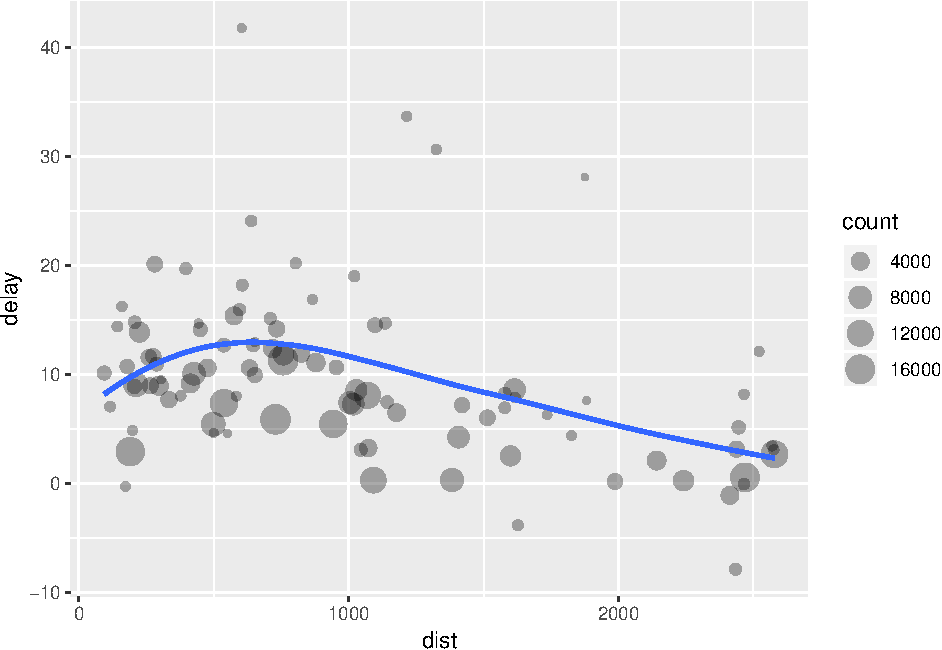
\includegraphics[width=0.7\linewidth]{EnvStat_files/figure-latex/distvsave-1} 

}

\caption{Jarak vs rata-rata delay}\label{fig:distvsave}
\end{figure}

Berdasarkan Figure \ref{fig:distvsave}, rata-rata delay meningkat
seiring dengan pertambahan jarak penerbangan.

\section{Referensi}\label{referensi-2}

\begin{enumerate}
\def\labelenumi{\arabic{enumi}.}
\tightlist
\item
  Wickham, H. Grolemund G. 2016. \textbf{R For Data Science: Import,
  Tidy, Transform, Visualize, And Model Data}. O'Reilly Media, Inc.
\item
  Peng, R.D. 2015. \textbf{Exploratory Data Analysis with R}. Leanpub
  book.
\item
  Dplyr Documentation. \url{https://dplyr.tidyverse.org/}
\item
  Quick-R. \textbf{Data Input}.
  \url{https://www.statmethods.net/input/index.html}
\item
  Quick-R. \textbf{Data Management}.
  \url{https://www.statmethods.net/management/index.html}
\item
  STHDA. \textbf{Importing Data Into R }.
  \url{http://www.sthda.com/english/wiki/importing-data-into-r}
\item
  STHDA. \textbf{Exporting Data From R}.
  \url{http://www.sthda.com/english/wiki/exporting-data-from-r}
\end{enumerate}

\chapter{Visualisasi Data Menggunakan Fungsi Dasar
R}\label{visualisasi-data-menggunakan-fungsi-dasar-r}

Visualisasi data merupakan bagian yang sangat penting untuk
mengkomunikasikan hasil analisa yang telah kita lakukan. Selain itu,
komunikasi juga membantu kita untuk memperoleh gambaran terkait data
selama proses analisa data sehingga membantu kita dalam memutuskan
metode analisa apa yang dapat kita terapkan pada data tersebut.

\texttt{R} memiliki library visualisasi yang sangat beragam, baik yang
merupakan fungsi dasar pada \texttt{R} maupun dari sumber lain seperti
ggplot dan lattice. Seluruh library visualisasi tersebut memiliki
kelebihan dan kekurangannya masing-masing.

Pada \emph{chapter} ini kita tidak akan membahas seluruh library
tersebut. Kita akab berfokus pada fungsi visualisasi dasar bawaan dari
\texttt{R}. kita akan mempelajari mengenai jenis visualisasi data sampai
dengan melakukan kustomisasi pada parameter grafik yang kita buat.

\section{Visualisasi Data Menggunakan Fungsi
plot()}\label{visualisasi-data-menggunakan-fungsi-plot}

Fungsi \texttt{plot()} merupakan fungsi umum yang digunakan untuk
membuat plot pada \texttt{R}. Format dasarnya adalah sebagai berikut:

\begin{Shaded}
\begin{Highlighting}[]
\KeywordTok{plot}\NormalTok{(x, y, }\DataTypeTok{type=}\StringTok{"p"}\NormalTok{)}
\end{Highlighting}
\end{Shaded}

\begin{quote}
\textbf{Note: }

\begin{itemize}
\tightlist
\item
  \textbf{x dan y}: titik koordinat plot Berupa variabel dengan panjang
  atau jumlah observasi yang sama.
\item
  \textbf{type}: jenis grafik yang hendak dibuat. Nilai yang dapat
  dimasukkan antara lain:
\item
  type=``p'' : membuat plot titik atau scatterplot. Nilai ini merupakan
  default pada fungsi \texttt{plot()}.
\item
  type=``l'' : membuat plot garis.
\item
  type=``b'' : membuat plot titik yang terhubung dengan garis.
\item
  type=``o'' : membuat plot titik yang ditimpa oleh garis.
\item
  type=``h'' : membuat plot garis vertikal dari titik ke garis y=0.
\item
  type=``s'' : membuat fungsi tangga.
\item
  type=``n'' : tidak membuat grafik plot sama sekali, kecuali plot dari
  axis. Dapat digunakan untuk mengatur tampilan suatu plot utama yang
  diikuti oleh sekelompok plot tambahan.
\end{itemize}
\end{quote}

Untuk lebih memahaminya berikut penulis akan sajikan contoh untuk
masing-masing grafik tersebut. Berikut adalah contoh sintaks dan hasil
plot yang disajikan pada Figure \ref{fig:plot}:

\begin{Shaded}
\begin{Highlighting}[]
\CommentTok{# membuat vektor data }
\NormalTok{x <-}\StringTok{ }\KeywordTok{c}\NormalTok{(}\DecValTok{1}\OperatorTok{:}\DecValTok{10}\NormalTok{); y <-}\StringTok{ }\NormalTok{x}\OperatorTok{^}\DecValTok{2}
\end{Highlighting}
\end{Shaded}

\begin{Shaded}
\begin{Highlighting}[]
\CommentTok{# membagi jendela grafik menajdi 4 baris dan 2 kolom}
\KeywordTok{par}\NormalTok{(}\DataTypeTok{mfrow=}\KeywordTok{c}\NormalTok{(}\DecValTok{3}\NormalTok{,}\DecValTok{3}\NormalTok{))}

\CommentTok{# loop}
\NormalTok{type <-}\StringTok{ }\KeywordTok{c}\NormalTok{(}\StringTok{"p"}\NormalTok{,}\StringTok{"l"}\NormalTok{,}\StringTok{"b"}\NormalTok{,}\StringTok{"o"}\NormalTok{,}\StringTok{"h"}\NormalTok{,}\StringTok{"s"}\NormalTok{,}\StringTok{"n"}\NormalTok{)}
\ControlFlowTok{for}\NormalTok{ (i }\ControlFlowTok{in}\NormalTok{ type)\{}
  \KeywordTok{plot}\NormalTok{(x,y, }\DataTypeTok{type=}\NormalTok{ i,}
       \DataTypeTok{main=} \KeywordTok{paste}\NormalTok{(}\StringTok{"type="}\NormalTok{, i))}
\NormalTok{\}}
\end{Highlighting}
\end{Shaded}

\begin{figure}

{\centering 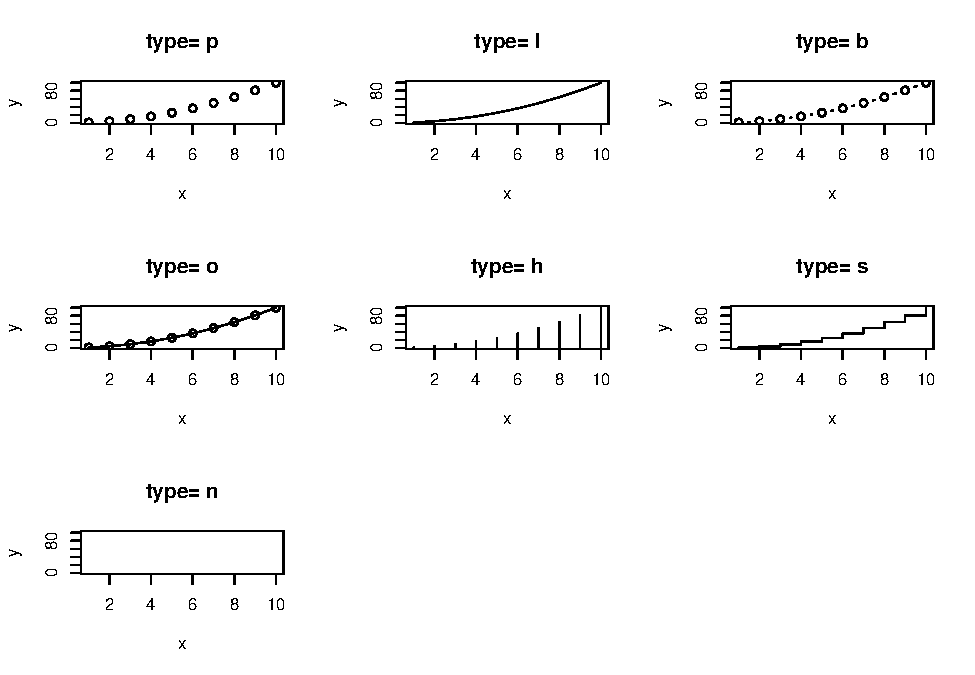
\includegraphics[width=0.8\linewidth]{EnvStat_files/figure-latex/plot-1} 

}

\caption{Plot berbagai jenis setting type}\label{fig:plot}
\end{figure}

Pada contoh selanjutnya akan dilakukan plot terhadap dataset
\texttt{trees}. Untuk memuatnya jalankan sintaks berikut:

\begin{Shaded}
\begin{Highlighting}[]
\KeywordTok{library}\NormalTok{(tibble)}
\end{Highlighting}
\end{Shaded}

\begin{Shaded}
\begin{Highlighting}[]
\CommentTok{# memuat dataset}
\NormalTok{trees <-}\StringTok{ }\KeywordTok{as_tibble}\NormalTok{(trees)}

\CommentTok{# print }
\NormalTok{trees}
\end{Highlighting}
\end{Shaded}

\begin{verbatim}
## # A tibble: 31 x 3
##    Girth Height Volume
##    <dbl>  <dbl>  <dbl>
##  1   8.3     70   10.3
##  2   8.6     65   10.3
##  3   8.8     63   10.2
##  4  10.5     72   16.4
##  5  10.7     81   18.8
##  6  10.8     83   19.7
##  7  11       66   15.6
##  8  11       75   18.2
##  9  11.1     80   22.6
## 10  11.2     75   19.9
## # ... with 21 more rows
\end{verbatim}

Pada dataset tersebut kita ingin membuat scatterplot untuk melihat
korelasi antara variabel \texttt{Height} dan \texttt{Volume}. Untuk
melakukannya jalankan sintaks berikut:

\begin{Shaded}
\begin{Highlighting}[]
\KeywordTok{plot}\NormalTok{(trees}\OperatorTok{$}\NormalTok{Height, trees}\OperatorTok{$}\NormalTok{Volume)}
\end{Highlighting}
\end{Shaded}

\begin{Shaded}
\begin{Highlighting}[]
\CommentTok{# atau }
\KeywordTok{with}\NormalTok{(trees, }\KeywordTok{plot}\NormalTok{(Height, Volume))}
\end{Highlighting}
\end{Shaded}

\begin{figure}

{\centering 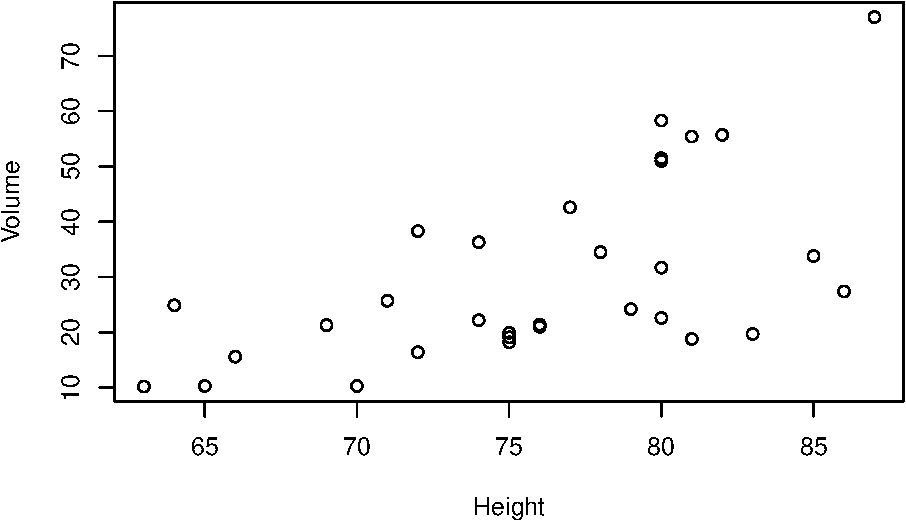
\includegraphics[width=0.7\linewidth]{EnvStat_files/figure-latex/scatter-1} 

}

\caption{Scatterplot Height vs Volume}\label{fig:scatter}
\end{figure}

Kita juga dapat menggunakan formula untuk membuat scatterplot pada
Figure \ref{fig:scatter}. Berikut adalah contoh sintaks yang digunakan:

\begin{Shaded}
\begin{Highlighting}[]
\NormalTok{x <-}\StringTok{ }\NormalTok{trees}\OperatorTok{$}\NormalTok{Height}
\NormalTok{y <-}\StringTok{ }\NormalTok{trees}\OperatorTok{$}\NormalTok{Volume}

\KeywordTok{plot}\NormalTok{(y}\OperatorTok{~}\NormalTok{x)}
\end{Highlighting}
\end{Shaded}

Fungsi \texttt{plot()} juga dapat digunakan untuk membentuk matriks
scatterplot. Untuk membuatnya kita hanya perlu memasukkan seluruh
dataset kedalam fungsi \texttt{plot()}. Berikut adalah sintaks dan
output yang dihasilkan berupa Figure \ref{fig:scatter2}:

\begin{Shaded}
\begin{Highlighting}[]
\KeywordTok{plot}\NormalTok{(trees)}
\end{Highlighting}
\end{Shaded}

\begin{figure}

{\centering 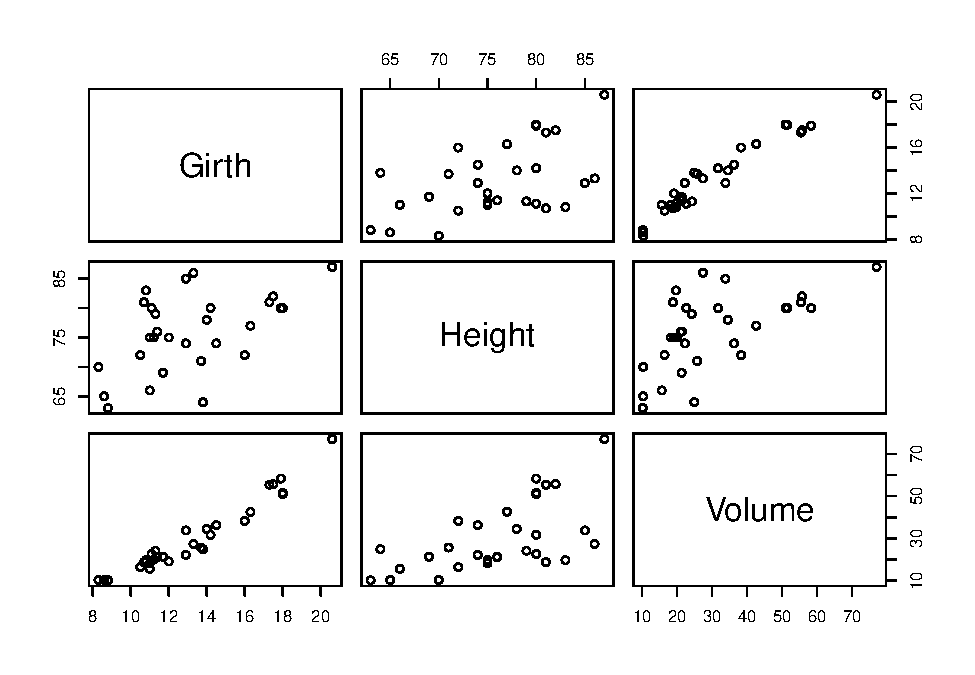
\includegraphics[width=0.8\linewidth]{EnvStat_files/figure-latex/scatter2-1} 

}

\caption{Matriks scatterplot dataset trees}\label{fig:scatter2}
\end{figure}

Selain itu jika kita memasukkan objek \texttt{lm()} yang merupakan
fungsi untuk melakukan operasi regresi linier pada fungsi
\texttt{plot()}, output yang dihasilkan berupa plot diagnostik yang
berguna untuk menguji asumsi model regresi linier. Berikut adalah contoh
sintaks dan output yang dihasilkan pada Figure \ref{fig:diag}:

\begin{Shaded}
\begin{Highlighting}[]
\CommentTok{# membagi jendela grafik menjadi 2 baris dan 2 kolom}
\KeywordTok{par}\NormalTok{(}\DataTypeTok{mfrow=}\KeywordTok{c}\NormalTok{(}\DecValTok{2}\NormalTok{,}\DecValTok{2}\NormalTok{))}

\CommentTok{# plot}
\KeywordTok{plot}\NormalTok{(}\KeywordTok{lm}\NormalTok{(Volume}\OperatorTok{~}\NormalTok{Height, }\DataTypeTok{data=}\NormalTok{trees))}
\end{Highlighting}
\end{Shaded}

\begin{figure}

{\centering 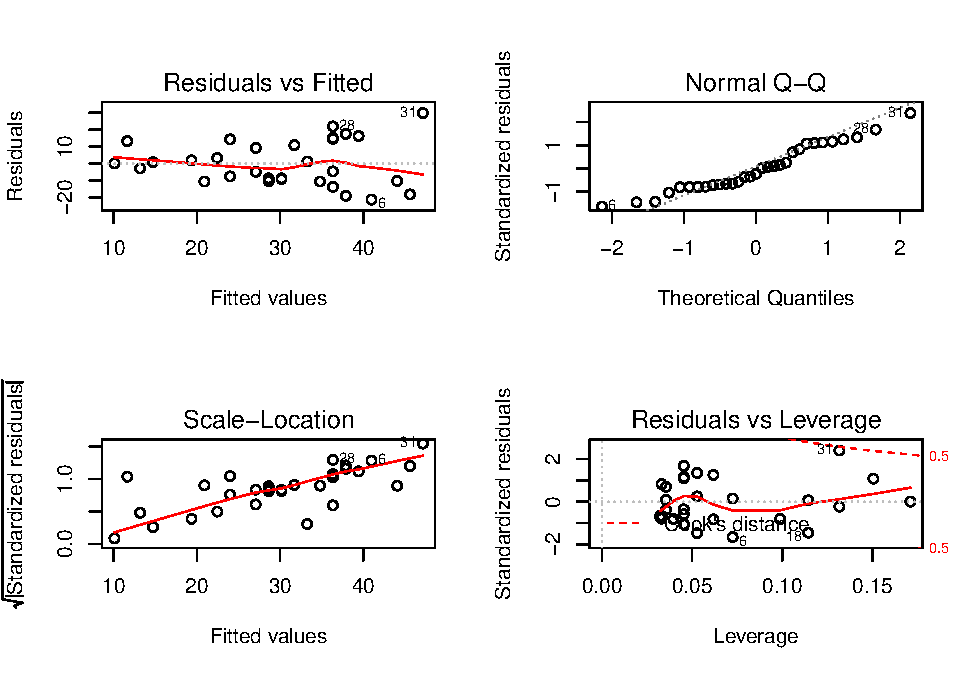
\includegraphics[width=0.8\linewidth]{EnvStat_files/figure-latex/diag-1} 

}

\caption{Plot diagnostik regresi linier}\label{fig:diag}
\end{figure}

Selain objek-objek tersebut, fungsi \texttt{plot()} akan banyak
digunakan dalam analisis statistika kita pada chapter lainnya.

\section{Matriks Scatterplot}\label{matriks-scatterplot}

Pada bagian sebelumnya kita telah belajar bagaimana membuat matriks
scatterplot mengggunakan fungsi \texttt{plot()}. Pada bagian ini kita
akan belajar cara membuat matriks scatterplot menggunakan fungsi
\texttt{pairs()}. Secara umum format fungsi dituliskan sebagai berikut:

\begin{Shaded}
\begin{Highlighting}[]
\KeywordTok{pairs}\NormalTok{(data, }\DataTypeTok{lower.panel=}\OtherTok{NULL}\NormalTok{)}
\end{Highlighting}
\end{Shaded}

\begin{quote}
\textbf{Note: }

\begin{itemize}
\tightlist
\item
  \textbf{data}: data frame
\item
  \textbf{lower.panel}: menampilkan atau tidak menampilkan panel bawah
\end{itemize}
\end{quote}

Untuk lebih memahami penggunaan fungsi tersebut, berikut akan disajikan
contoh penggunaannya pada dataset \texttt{iris}. Sebelum melakukannya
jalankan sintaks berikut untuk memuat dataset:

\begin{Shaded}
\begin{Highlighting}[]
\CommentTok{# memuat dataset irir}
\NormalTok{iris <-}\StringTok{ }\KeywordTok{as_tibble}\NormalTok{(iris)}

\CommentTok{# print}
\NormalTok{iris}
\end{Highlighting}
\end{Shaded}

\begin{verbatim}
## # A tibble: 150 x 5
##    Sepal.Length Sepal.Width Petal.Length Petal.Width Species
##           <dbl>       <dbl>        <dbl>       <dbl> <fct>  
##  1          5.1         3.5          1.4         0.2 setosa 
##  2          4.9         3            1.4         0.2 setosa 
##  3          4.7         3.2          1.3         0.2 setosa 
##  4          4.6         3.1          1.5         0.2 setosa 
##  5          5           3.6          1.4         0.2 setosa 
##  6          5.4         3.9          1.7         0.4 setosa 
##  7          4.6         3.4          1.4         0.3 setosa 
##  8          5           3.4          1.5         0.2 setosa 
##  9          4.4         2.9          1.4         0.2 setosa 
## 10          4.9         3.1          1.5         0.1 setosa 
## # ... with 140 more rows
\end{verbatim}

Untuk membuat matriks scatterplot kita hanya perlu memasukkan objek
\texttt{iris} kedalam fungsi \texttt{pairs()}. Berikut adalah sintaks
yang digunakan dan output yang dihasilkan pada Figure \ref{fig:matscat}:

\begin{Shaded}
\begin{Highlighting}[]
\KeywordTok{pairs}\NormalTok{(iris)}
\end{Highlighting}
\end{Shaded}

\begin{figure}

{\centering 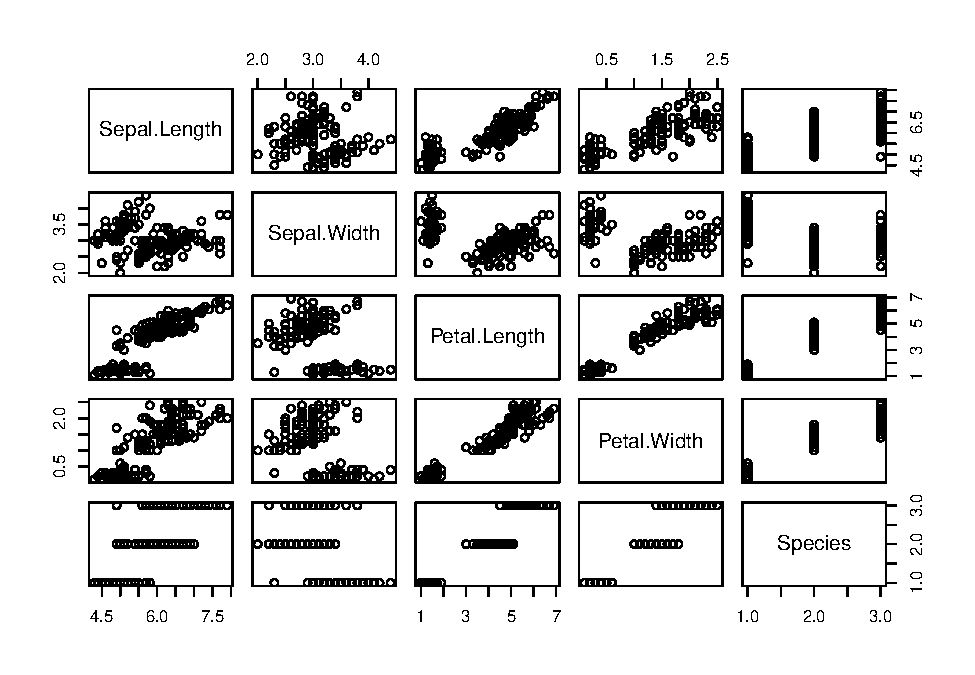
\includegraphics[width=0.8\linewidth]{EnvStat_files/figure-latex/matscat-1} 

}

\caption{Matriks scatterplot iris}\label{fig:matscat}
\end{figure}

Kita dapat melakukan drop terhadap panel bawah grafik tersebut. Untuk
melakukannya kita perlu memasukkan parameter \texttt{lower.panel=NULL}.
Output yang dihasilkan akan tampak seperti pada Figure
\ref{fig:matscat2}.

\begin{Shaded}
\begin{Highlighting}[]
\KeywordTok{pairs}\NormalTok{(iris, }\DataTypeTok{lower.panel=}\OtherTok{NULL}\NormalTok{)}
\end{Highlighting}
\end{Shaded}

\begin{figure}

{\centering 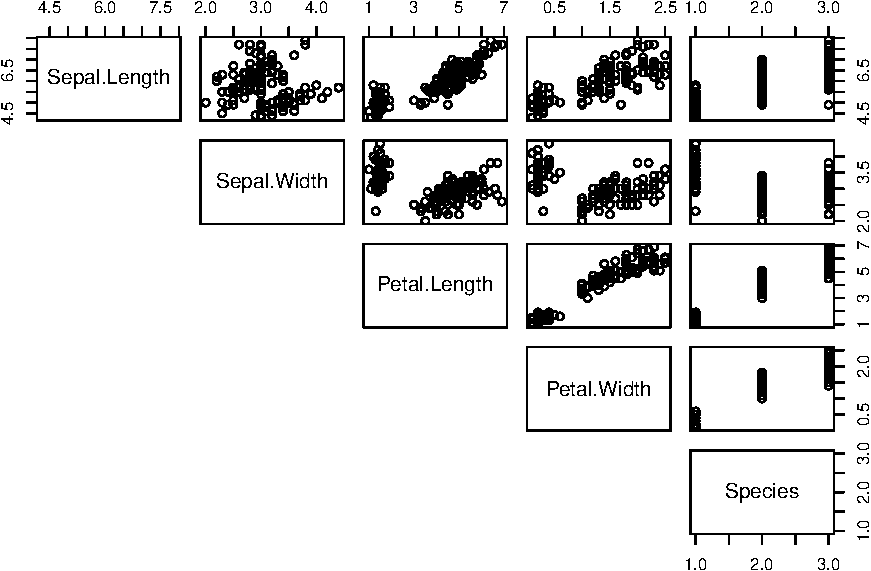
\includegraphics[width=0.8\linewidth]{EnvStat_files/figure-latex/matscat2-1} 

}

\caption{Matriks scatterplot iris tanpa panel bawah}\label{fig:matscat2}
\end{figure}

Kita dapat merubah warna titik berdasarkan factor \texttt{Species}.
Langkah pertama yang perlu dilakukan adalah melakukan drop variabel
\texttt{Species} pada dataset dan memasukkan objek baru tanpa variabel
tersebut kedalam fungsi \texttt{pairs()}. Warna berdasarkan grup
diberikan dengan menambahkan parameter \texttt{col=} pada fungsi
\texttt{pairs()}. Berikut adalah contoh penerapannya dan output yang
dihasilkan pada Figure \ref{fig:matscat3}:

\begin{Shaded}
\begin{Highlighting}[]
\CommentTok{# drop variabel Species}
\CommentTok{# simpan dataset baru pada objek iris2}
\NormalTok{iris2 <-}\StringTok{ }\NormalTok{iris[ ,}\DecValTok{1}\OperatorTok{:}\DecValTok{4}\NormalTok{]}

\CommentTok{# print}
\NormalTok{iris2}
\end{Highlighting}
\end{Shaded}

\begin{verbatim}
## # A tibble: 150 x 4
##    Sepal.Length Sepal.Width Petal.Length Petal.Width
##           <dbl>       <dbl>        <dbl>       <dbl>
##  1          5.1         3.5          1.4         0.2
##  2          4.9         3            1.4         0.2
##  3          4.7         3.2          1.3         0.2
##  4          4.6         3.1          1.5         0.2
##  5          5           3.6          1.4         0.2
##  6          5.4         3.9          1.7         0.4
##  7          4.6         3.4          1.4         0.3
##  8          5           3.4          1.5         0.2
##  9          4.4         2.9          1.4         0.2
## 10          4.9         3.1          1.5         0.1
## # ... with 140 more rows
\end{verbatim}

\begin{Shaded}
\begin{Highlighting}[]
\CommentTok{# spesifikasi vaktor warna titik berdasarkan spesies}
\NormalTok{my_col <-}\StringTok{ }\KeywordTok{c}\NormalTok{(}\StringTok{"#00AFBB"}\NormalTok{, }\StringTok{"#E7B800"}\NormalTok{, }\StringTok{"#FC4E07"}\NormalTok{)}

\CommentTok{# plot}
\KeywordTok{pairs}\NormalTok{(iris2, }\DataTypeTok{lower.panel=}\OtherTok{NULL}\NormalTok{,}
      \CommentTok{# spesifikasi warna}
      \DataTypeTok{col=}\NormalTok{ my_col[iris}\OperatorTok{$}\NormalTok{Species])}
\end{Highlighting}
\end{Shaded}

\begin{figure}

{\centering 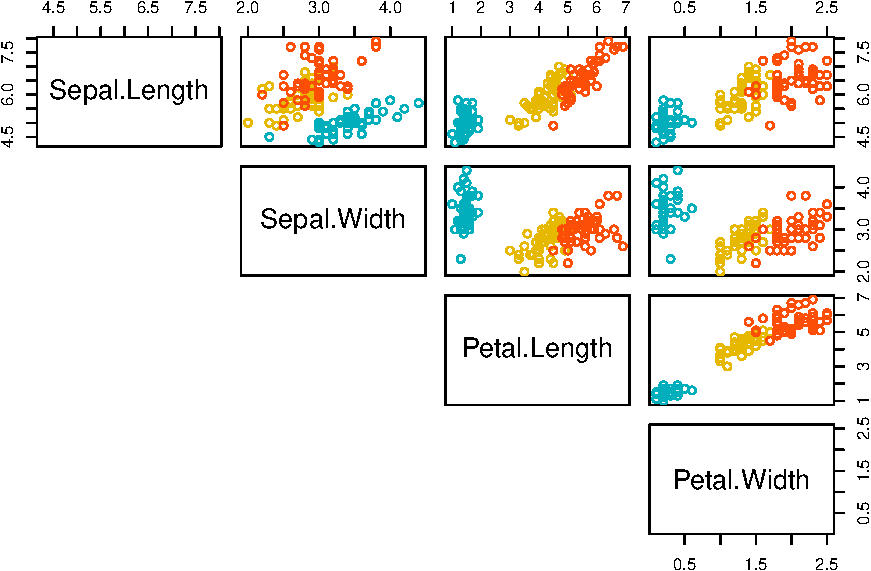
\includegraphics[width=0.8\linewidth]{EnvStat_files/figure-latex/matscat3-1} 

}

\caption{Matriks scatterplot iris tanpa panel bawah}\label{fig:matscat3}
\end{figure}

Kita juga dapat mengganti panel bawah menjadi nilai korelasi antar
variabel. Untuk melakukannya kita perlu mendefinisikan sebuah fungsi
untuk panel bawah dan panel atas (jika ingin warna titik berdasarkan
factor). Setelah fungsi panel bawah dan atas didefinisikan, langkah
selanjutnya adalah melakukan memasukkan nilainya kedalam fungsi
\texttt{pairs()}. Berikut adalah sintaks yang digunakan serta output
yang dihasilkan pada Figure \ref{fig:matscat4}:

\begin{Shaded}
\begin{Highlighting}[]
\CommentTok{# membuat fungsi untuk menghitung}
\CommentTok{# nilai korelasi yang ditempatkan pada panel bawah}
\NormalTok{panel.cor <-}\StringTok{ }\ControlFlowTok{function}\NormalTok{(x, y)\{}
    \CommentTok{# definisi parameter grafik }
\NormalTok{    usr <-}\StringTok{ }\KeywordTok{par}\NormalTok{(}\StringTok{"usr"}\NormalTok{); }\KeywordTok{on.exit}\NormalTok{(}\KeywordTok{par}\NormalTok{(usr))}
    \KeywordTok{par}\NormalTok{(}\DataTypeTok{usr =} \KeywordTok{c}\NormalTok{(}\DecValTok{0}\NormalTok{, }\DecValTok{1}\NormalTok{, }\DecValTok{0}\NormalTok{, }\DecValTok{1}\NormalTok{))}
    \CommentTok{# menghitung koefisien korelas}
\NormalTok{    r <-}\StringTok{ }\KeywordTok{round}\NormalTok{(}\KeywordTok{cor}\NormalTok{(x, y), }\DataTypeTok{digits=}\DecValTok{2}\NormalTok{)}
    \CommentTok{# menambahkan text berdasarkan koefisien korelasi}
\NormalTok{    txt <-}\StringTok{ }\KeywordTok{paste0}\NormalTok{(}\StringTok{"R = "}\NormalTok{, r)}
    \CommentTok{# mengatur besar text sesuai besarnya nilai korelasi}
\NormalTok{    cex.cor <-}\StringTok{ }\FloatTok{0.8}\OperatorTok{/}\KeywordTok{strwidth}\NormalTok{(txt)}
    \KeywordTok{text}\NormalTok{(}\FloatTok{0.5}\NormalTok{, }\FloatTok{0.5}\NormalTok{, txt, }\DataTypeTok{cex =}\NormalTok{ cex.cor }\OperatorTok{*}\StringTok{ }\KeywordTok{abs}\NormalTok{(r))}
\NormalTok{\}}

\CommentTok{# kustomisasi panel atas agar}
\CommentTok{# warna titik berdasarkan factor}
\NormalTok{my_col <-}\StringTok{ }\KeywordTok{c}\NormalTok{(}\StringTok{"#00AFBB"}\NormalTok{, }\StringTok{"#E7B800"}\NormalTok{, }\StringTok{"#FC4E07"}\NormalTok{)}
\NormalTok{upper.panel<-}\ControlFlowTok{function}\NormalTok{(x, y)\{}
  \KeywordTok{points}\NormalTok{(x,y, }\DataTypeTok{col =}\NormalTok{ my_col[iris}\OperatorTok{$}\NormalTok{Species])}
\NormalTok{\}}

\KeywordTok{pairs}\NormalTok{(iris2,}
      \DataTypeTok{lower.panel=}\NormalTok{ panel.cor,}
      \DataTypeTok{upper.panel=}\NormalTok{ upper.panel)}
\end{Highlighting}
\end{Shaded}

\begin{figure}

{\centering 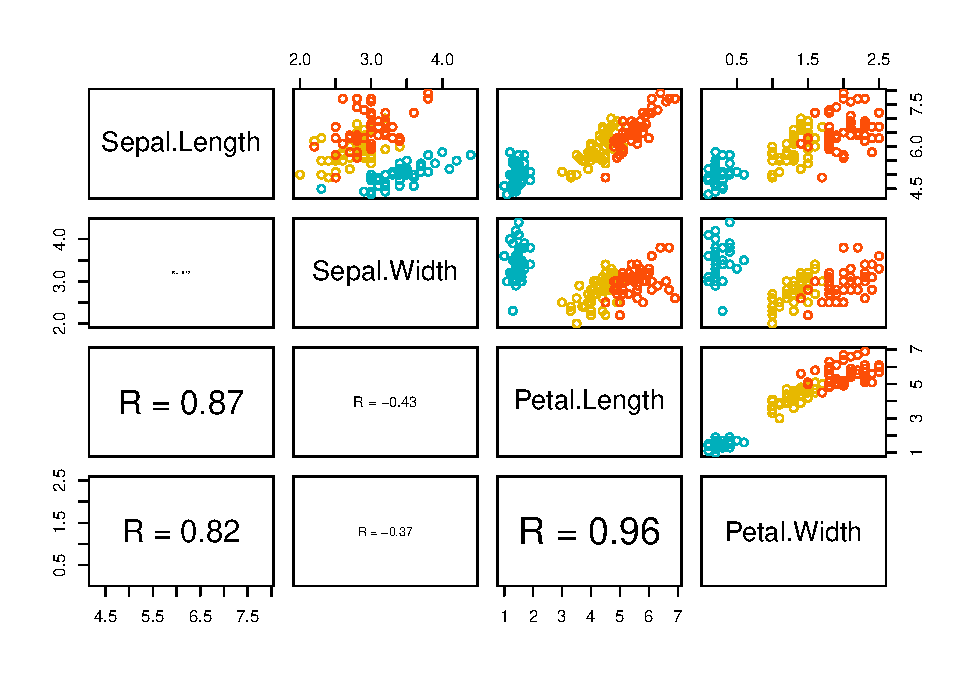
\includegraphics[width=0.8\linewidth]{EnvStat_files/figure-latex/matscat4-1} 

}

\caption{Matriks scatterplot iris dengan koefisien korelasi}\label{fig:matscat4}
\end{figure}

Jika kita tidak ingin nilai korelasi ditampilkan di panel bawah, kita
dapat merubahnya sehingga dapat tampil pada panel atas bersamaan dengan
scatterplot. Untuk melakukannya kita perlu mendefinisikan fungsi pada
panel atas dan memasukkannya pada parameter \texttt{upper.panel=}.
Berikut adalah sintaks yang digunakan beserta output yang dihasilkan
pada Figure \ref{fig:matscat5}:

\begin{Shaded}
\begin{Highlighting}[]
\CommentTok{# kustomisasi panel atas}
\NormalTok{upper.panel<-}\ControlFlowTok{function}\NormalTok{(x, y)\{}
  \KeywordTok{points}\NormalTok{(x,y, }\DataTypeTok{col=}\KeywordTok{c}\NormalTok{(}\StringTok{"#00AFBB"}\NormalTok{, }\StringTok{"#E7B800"}\NormalTok{, }\StringTok{"#FC4E07"}\NormalTok{)[iris}\OperatorTok{$}\NormalTok{Species])}
\NormalTok{  r <-}\StringTok{ }\KeywordTok{round}\NormalTok{(}\KeywordTok{cor}\NormalTok{(x, y), }\DataTypeTok{digits=}\DecValTok{2}\NormalTok{)}
\NormalTok{  txt <-}\StringTok{ }\KeywordTok{paste0}\NormalTok{(}\StringTok{"R = "}\NormalTok{, r)}
\NormalTok{  usr <-}\StringTok{ }\KeywordTok{par}\NormalTok{(}\StringTok{"usr"}\NormalTok{); }\KeywordTok{on.exit}\NormalTok{(}\KeywordTok{par}\NormalTok{(usr))}
  \KeywordTok{par}\NormalTok{(}\DataTypeTok{usr =} \KeywordTok{c}\NormalTok{(}\DecValTok{0}\NormalTok{, }\DecValTok{1}\NormalTok{, }\DecValTok{0}\NormalTok{, }\DecValTok{1}\NormalTok{))}
  \KeywordTok{text}\NormalTok{(}\FloatTok{0.5}\NormalTok{, }\FloatTok{0.9}\NormalTok{, txt)}
\NormalTok{\}}

\CommentTok{# plot}
\KeywordTok{pairs}\NormalTok{(iris2, }\DataTypeTok{lower.panel =} \OtherTok{NULL}\NormalTok{, }
      \DataTypeTok{upper.panel =}\NormalTok{ upper.panel)}
\end{Highlighting}
\end{Shaded}

\begin{figure}

{\centering 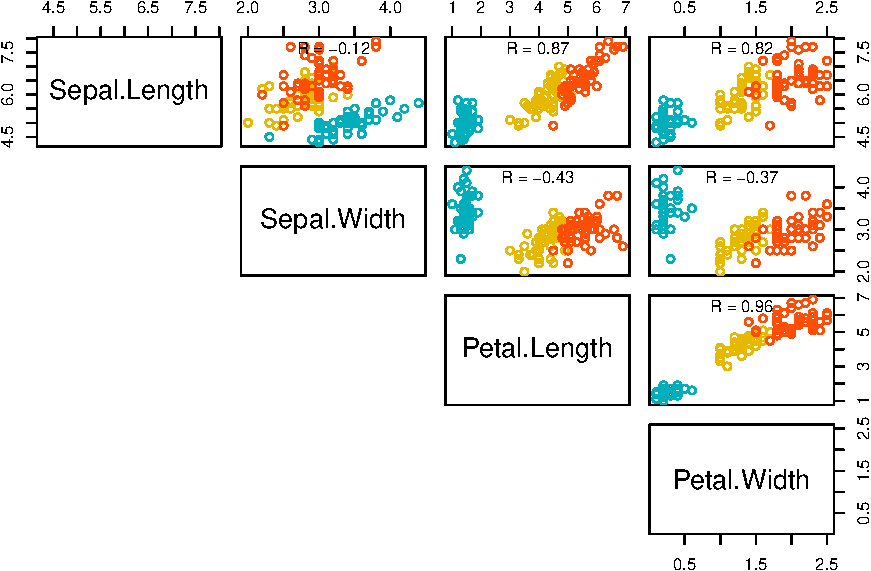
\includegraphics[width=0.8\linewidth]{EnvStat_files/figure-latex/matscat5-1} 

}

\caption{Matriks scatterplot iris dengan koefisien korelasi di panel atas}\label{fig:matscat5}
\end{figure}

\section{Box plot}\label{box-plot}

Box plot pada \texttt{R} dapat dibuat menggunakan fungsi
\texttt{boxplot()}. Berikut adalah sintaks untuk membuat boxplot
variabel \texttt{Sepal.Lenght} pada dataset \texttt{iris} dan output
yang dihasilkan pada Figure \ref{fig:boxplot}:

\begin{Shaded}
\begin{Highlighting}[]
\KeywordTok{boxplot}\NormalTok{(iris}\OperatorTok{$}\NormalTok{Sepal.Length)}
\end{Highlighting}
\end{Shaded}

\begin{figure}

{\centering 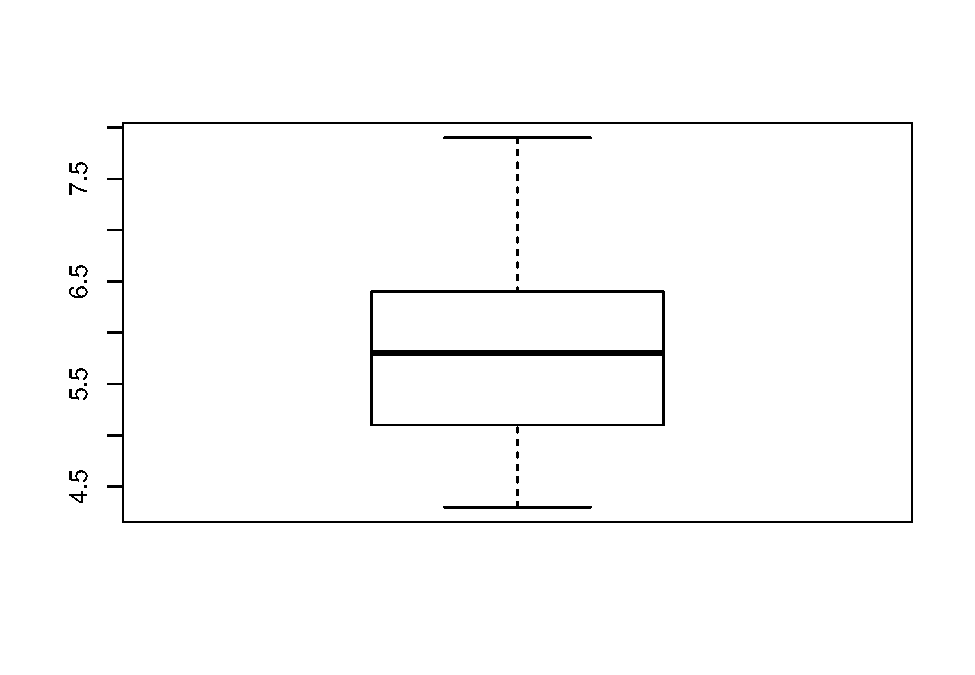
\includegraphics[width=0.7\linewidth]{EnvStat_files/figure-latex/boxplot-1} 

}

\caption{Boxplot variabel Sepal.Length}\label{fig:boxplot}
\end{figure}

Boxplot juga dapat dibuat berdasarkan variabel factor. Hal ini berguna
untuk melihat perbedaan ditribusi data pada masing-masing grup. Pada
sintaks berikut dibuat boxplot berdasarkan variabel \texttt{Species}.
Output yang dihasilkan disajikan pada Figure \ref{fig:boxplot2}:

\begin{Shaded}
\begin{Highlighting}[]
\KeywordTok{boxplot}\NormalTok{(iris}\OperatorTok{$}\NormalTok{Sepal.Length}\OperatorTok{~}\NormalTok{iris}\OperatorTok{$}\NormalTok{Species)}
\end{Highlighting}
\end{Shaded}

\begin{figure}

{\centering 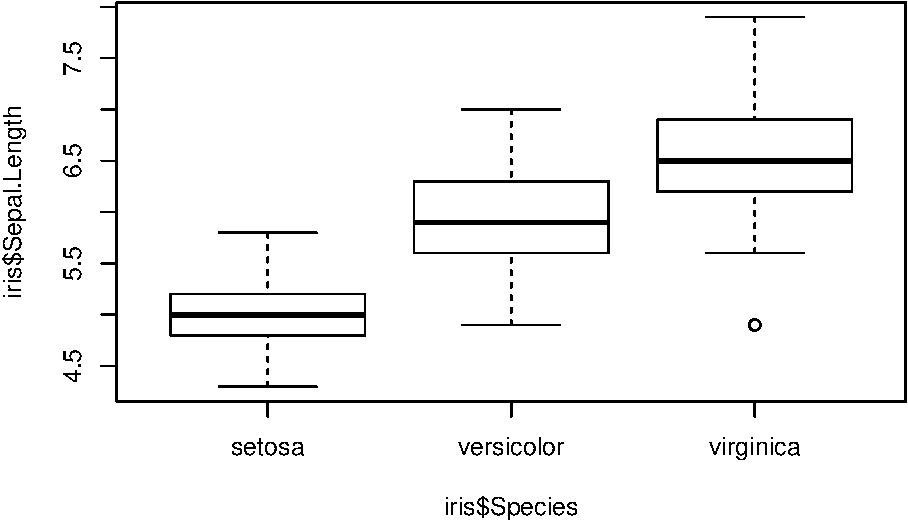
\includegraphics[width=0.7\linewidth]{EnvStat_files/figure-latex/boxplot2-1} 

}

\caption{Boxplot berdasarkan variabel species}\label{fig:boxplot2}
\end{figure}

Kita juga dapat mengubah warna outline dan box pada boxplot. Berikut
adalah contoh sintaks yang digunakan untuk melakukannya dan output yang
dihasilkan disajikan pada Figure \ref{fig:boxplot3}:

\begin{Shaded}
\begin{Highlighting}[]
\KeywordTok{boxplot}\NormalTok{(iris}\OperatorTok{$}\NormalTok{Sepal.Length}\OperatorTok{~}\NormalTok{iris}\OperatorTok{$}\NormalTok{Species,}
        \CommentTok{# ubah warna outline menjadi steelblue}
        \DataTypeTok{border =} \StringTok{"steelblue"}\NormalTok{,}
        \CommentTok{# ubah warna box berdasarkan grup}
        \DataTypeTok{col=} \KeywordTok{c}\NormalTok{(}\StringTok{"#999999"}\NormalTok{, }\StringTok{"#E69F00"}\NormalTok{, }\StringTok{"#56B4E9"}\NormalTok{))}
\end{Highlighting}
\end{Shaded}

\begin{figure}

{\centering 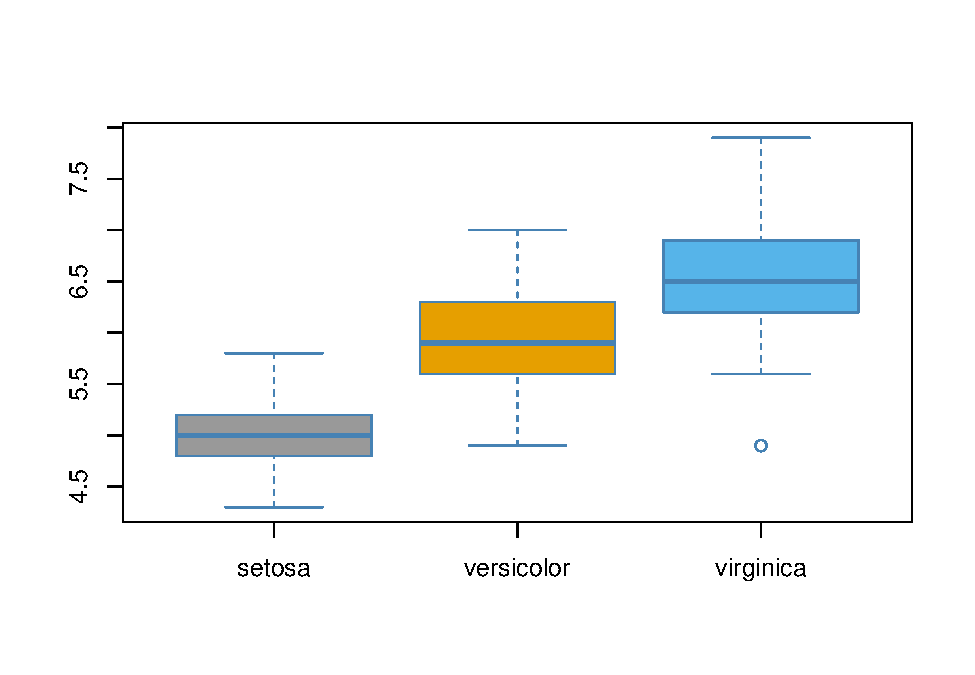
\includegraphics[width=0.7\linewidth]{EnvStat_files/figure-latex/boxplot3-1} 

}

\caption{Boxplot dengan warna berdasarkan spesies}\label{fig:boxplot3}
\end{figure}

Kita juga dapat membuat boxplot pada \emph{multiple group}. Data yang
digunakan untuk contoh tersebut adalah dataset \texttt{ToothGrowth}.
Berikut adalah sintaks untuk memuat dataset tersebut:

\begin{Shaded}
\begin{Highlighting}[]
\CommentTok{# memuat dataset sebagai tibble}
\NormalTok{ToothGrowth <-}\StringTok{ }\KeywordTok{as_tibble}\NormalTok{(ToothGrowth)}

\CommentTok{# print}
\NormalTok{ToothGrowth}
\end{Highlighting}
\end{Shaded}

\begin{verbatim}
## # A tibble: 60 x 3
##      len supp   dose
##    <dbl> <fct> <dbl>
##  1   4.2 VC      0.5
##  2  11.5 VC      0.5
##  3   7.3 VC      0.5
##  4   5.8 VC      0.5
##  5   6.4 VC      0.5
##  6  10   VC      0.5
##  7  11.2 VC      0.5
##  8  11.2 VC      0.5
##  9   5.2 VC      0.5
## 10   7   VC      0.5
## # ... with 50 more rows
\end{verbatim}

\begin{Shaded}
\begin{Highlighting}[]
\CommentTok{# ubah variable dose menjadi factor}
\NormalTok{ToothGrowth}\OperatorTok{$}\NormalTok{dose <-}\StringTok{ }\KeywordTok{as.factor}\NormalTok{(ToothGrowth}\OperatorTok{$}\NormalTok{dose)}

\CommentTok{# print}
\NormalTok{ToothGrowth}
\end{Highlighting}
\end{Shaded}

\begin{verbatim}
## # A tibble: 60 x 3
##      len supp  dose 
##    <dbl> <fct> <fct>
##  1   4.2 VC    0.5  
##  2  11.5 VC    0.5  
##  3   7.3 VC    0.5  
##  4   5.8 VC    0.5  
##  5   6.4 VC    0.5  
##  6  10   VC    0.5  
##  7  11.2 VC    0.5  
##  8  11.2 VC    0.5  
##  9   5.2 VC    0.5  
## 10   7   VC    0.5  
## # ... with 50 more rows
\end{verbatim}

Contoh sintaks dan output boxplot \emph{multiple group} disajikan pada
Figure \ref{fig:boxplot4}:

\begin{Shaded}
\begin{Highlighting}[]
\KeywordTok{boxplot}\NormalTok{(len }\OperatorTok{~}\StringTok{ }\NormalTok{supp}\OperatorTok{*}\NormalTok{dose, }\DataTypeTok{data =}\NormalTok{ ToothGrowth,}
        \DataTypeTok{col =} \KeywordTok{c}\NormalTok{(}\StringTok{"white"}\NormalTok{, }\StringTok{"steelblue"}\NormalTok{))}
\end{Highlighting}
\end{Shaded}

\begin{figure}

{\centering 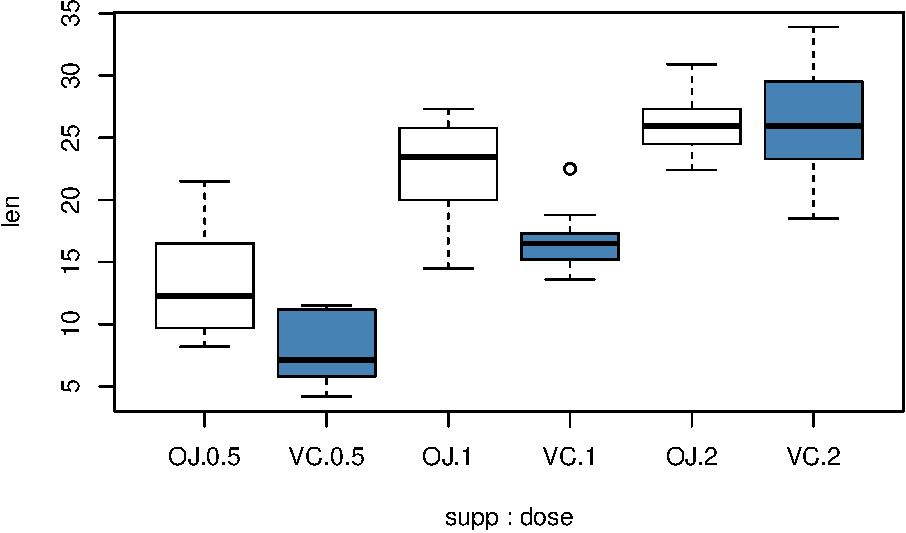
\includegraphics[width=0.7\linewidth]{EnvStat_files/figure-latex/boxplot4-1} 

}

\caption{Boxplot multiple group}\label{fig:boxplot4}
\end{figure}

\section{Bar Plot}\label{bar-plot}

Barplot pada \texttt{R} dapat dibuat menggunakan fungsi
\texttt{barplot()}. Untuk lebih memahaminya berikut disajikan contoh
barplot menggunakan dataset \texttt{VADeaths}. Untuk memuatnya jalankan
sintaks berikut:

\begin{Shaded}
\begin{Highlighting}[]
\NormalTok{VADeaths}
\end{Highlighting}
\end{Shaded}

\begin{verbatim}
##       Rural Male Rural Female Urban Male Urban Female
## 50-54       11.7          8.7       15.4          8.4
## 55-59       18.1         11.7       24.3         13.6
## 60-64       26.9         20.3       37.0         19.3
## 65-69       41.0         30.9       54.6         35.1
## 70-74       66.0         54.3       71.1         50.0
\end{verbatim}

Contoh bar plot untuk variabel \texttt{Rural\ Male} disajikan pada
Figure \ref{fig:barplot}:

\begin{Shaded}
\begin{Highlighting}[]
\KeywordTok{par}\NormalTok{(}\DataTypeTok{mfrow=}\KeywordTok{c}\NormalTok{(}\DecValTok{1}\NormalTok{,}\DecValTok{2}\NormalTok{))}
\KeywordTok{barplot}\NormalTok{(VADeaths[, }\StringTok{"Rural Male"}\NormalTok{], }\DataTypeTok{main=}\StringTok{"a"}\NormalTok{)}
\KeywordTok{barplot}\NormalTok{(VADeaths[, }\StringTok{"Rural Male"}\NormalTok{], }\DataTypeTok{main=}\StringTok{"b"}\NormalTok{, }\DataTypeTok{horiz=}\OtherTok{TRUE}\NormalTok{)}
\end{Highlighting}
\end{Shaded}

\begin{figure}

{\centering 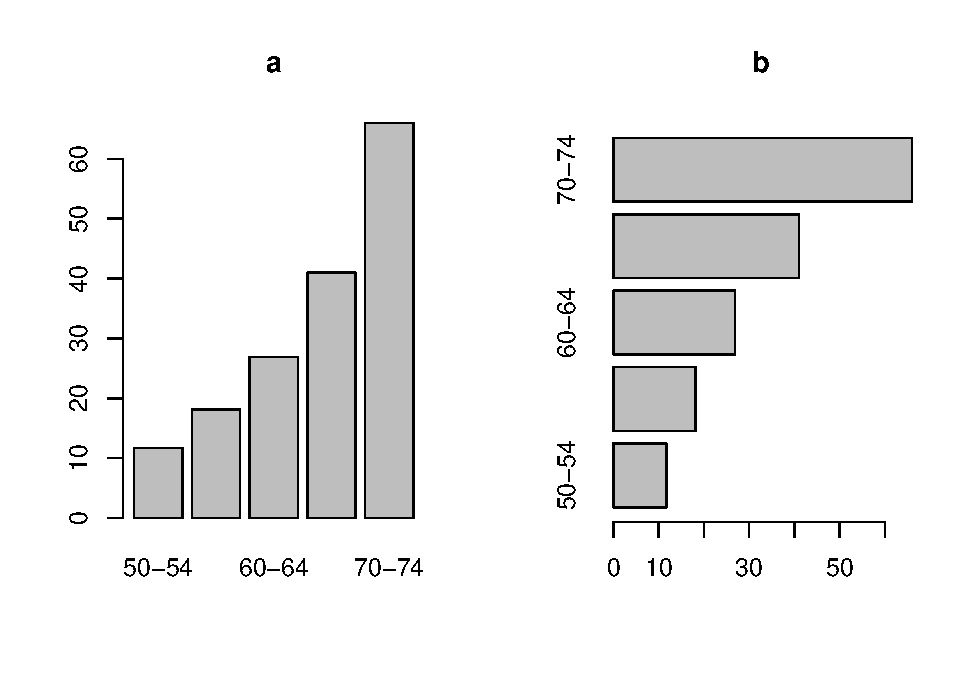
\includegraphics[width=0.7\linewidth]{EnvStat_files/figure-latex/barplot-1} 

}

\caption{a. bar plot vertikal; b. bar plot horizontal}\label{fig:barplot}
\end{figure}

\begin{Shaded}
\begin{Highlighting}[]
\KeywordTok{par}\NormalTok{(}\DataTypeTok{mfrow=}\KeywordTok{c}\NormalTok{(}\DecValTok{1}\NormalTok{,}\DecValTok{1}\NormalTok{))}
\end{Highlighting}
\end{Shaded}

Kita dapat mengubah warna pada masing-masing bar, baik outline bar
maupun box pada bar. Selain itu kita juga dapat mengubah nama grup yang
telah dihasilkan sebelumnya. Berikut sintaks untuk melakukannya dan
output yang dihasilkan pada Figure \ref{fig:barplot2}:

\begin{Shaded}
\begin{Highlighting}[]
\KeywordTok{barplot}\NormalTok{(VADeaths[, }\StringTok{"Rural Male"}\NormalTok{],}
        \CommentTok{# ubah warna ouline menjadi steelblue}
        \DataTypeTok{border=}\StringTok{"steelblue"}\NormalTok{,}
        \CommentTok{# ubah wana box}
        \DataTypeTok{col=} \KeywordTok{c}\NormalTok{(}\StringTok{"grey"}\NormalTok{, }\StringTok{"yellow"}\NormalTok{, }\StringTok{"steelblue"}\NormalTok{, }\StringTok{"green"}\NormalTok{, }\StringTok{"orange"}\NormalTok{),}
        \CommentTok{# ubah nama grup dari A sampai E}
        \DataTypeTok{names.arg =}\NormalTok{ LETTERS[}\DecValTok{1}\OperatorTok{:}\DecValTok{5}\NormalTok{],}
        \CommentTok{# ubah orientasi menajadi horizontal}
        \DataTypeTok{horiz=}\OtherTok{TRUE}\NormalTok{)}
\end{Highlighting}
\end{Shaded}

\begin{figure}

{\centering 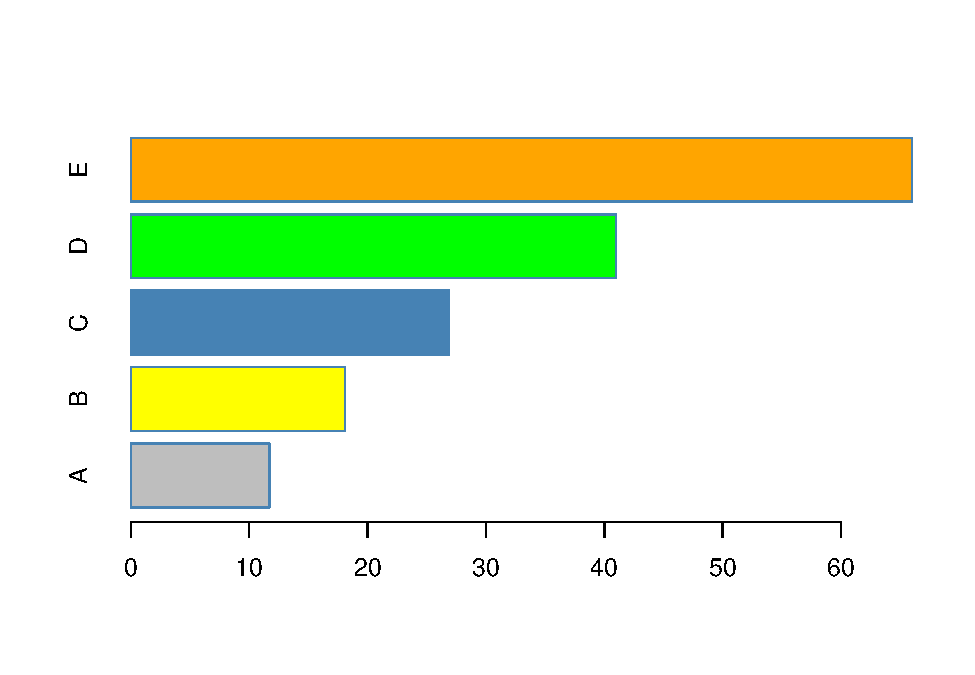
\includegraphics[width=0.7\linewidth]{EnvStat_files/figure-latex/barplot2-1} 

}

\caption{Kustomisasi bar plot}\label{fig:barplot2}
\end{figure}

Untuk bar plot dengan \emph{multiple group}, tersedia dua pengaturan
posisi yaitu \emph{stacked bar plot}(menunjukkan proporsi penyusun pada
masing-masing grup) dan \emph{grouped bar plot}(melihat perbedaan
individual pada masing-masing grup). Pada Figure \ref{fig:barplot3} dan
Figure \ref{fig:barplot4} , disajikan kedua jenis bar plot tersebut.

\begin{Shaded}
\begin{Highlighting}[]
\CommentTok{# staked}
\KeywordTok{barplot}\NormalTok{(VADeaths,}
         \DataTypeTok{col =} \KeywordTok{c}\NormalTok{(}\StringTok{"lightblue"}\NormalTok{, }\StringTok{"mistyrose"}\NormalTok{, }\StringTok{"lightcyan"}\NormalTok{, }
                 \StringTok{"lavender"}\NormalTok{, }\StringTok{"cornsilk"}\NormalTok{),}
        \DataTypeTok{legend =} \KeywordTok{rownames}\NormalTok{(VADeaths))}
\end{Highlighting}
\end{Shaded}

\begin{figure}

{\centering 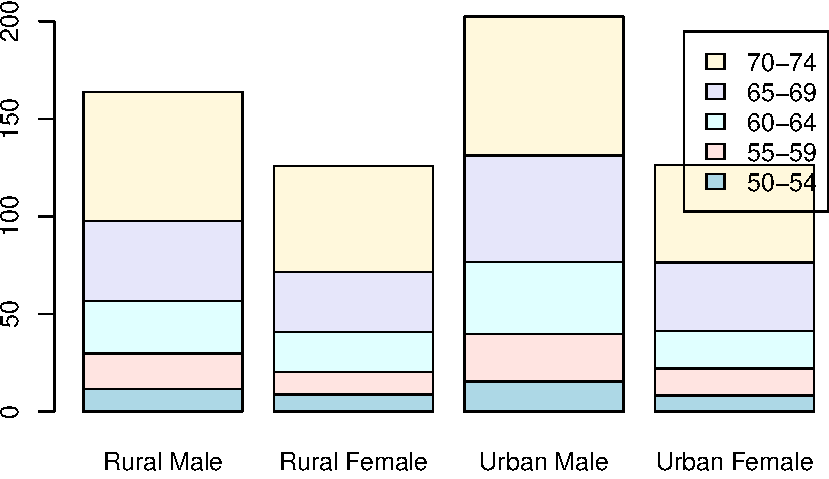
\includegraphics[width=0.7\linewidth]{EnvStat_files/figure-latex/barplot3-1} 

}

\caption{Stacked bar plot}\label{fig:barplot3}
\end{figure}

\begin{Shaded}
\begin{Highlighting}[]
\CommentTok{# grouped}
\KeywordTok{barplot}\NormalTok{(VADeaths,}
         \DataTypeTok{col =} \KeywordTok{c}\NormalTok{(}\StringTok{"lightblue"}\NormalTok{, }\StringTok{"mistyrose"}\NormalTok{, }\StringTok{"lightcyan"}\NormalTok{, }
                 \StringTok{"lavender"}\NormalTok{, }\StringTok{"cornsilk"}\NormalTok{),}
        \DataTypeTok{legend =} \KeywordTok{rownames}\NormalTok{(VADeaths), }\DataTypeTok{beside =} \OtherTok{TRUE}\NormalTok{)}
\end{Highlighting}
\end{Shaded}

\begin{figure}

{\centering 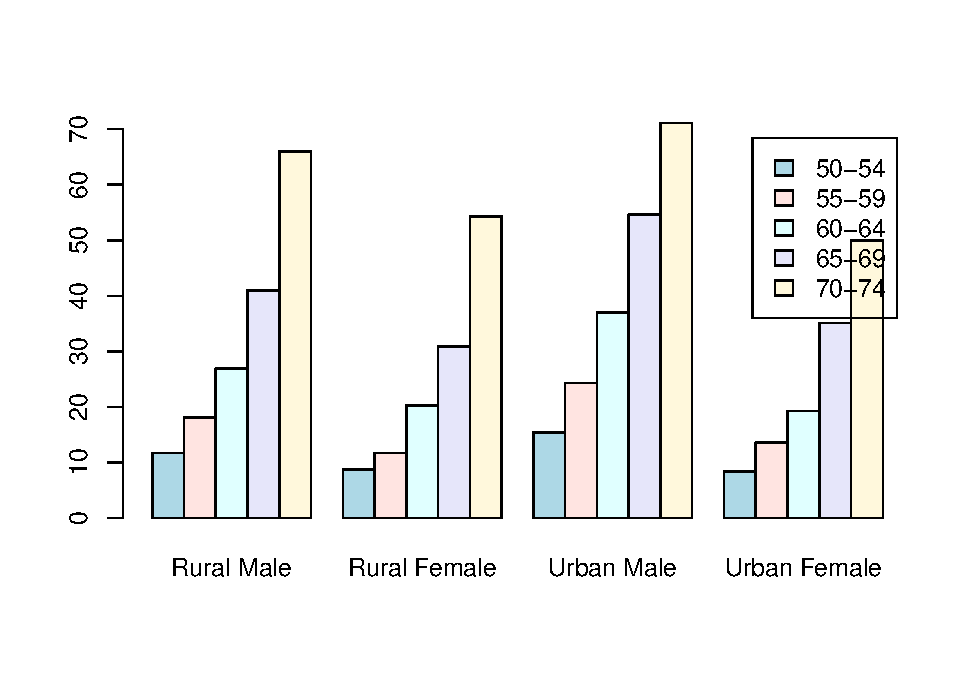
\includegraphics[width=0.7\linewidth]{EnvStat_files/figure-latex/barplot4-1} 

}

\caption{Grouped bar plot}\label{fig:barplot4}
\end{figure}

\section{Line Plot}\label{line-plot}

Line plot pada \texttt{R} dapat dibentuk menggunakan fungsi
\texttt{plot()}. Selain itu fungsi \texttt{lines()} dapat pula digunakan
untuk menambahkan line plot pada grafik. Berikut adalah sintaks untuk
membuat line plot dan outputnya pada Figure \ref{fig:line}:

\begin{Shaded}
\begin{Highlighting}[]
\CommentTok{# Membuat vektor data}
\NormalTok{x <-}\StringTok{ }\KeywordTok{c}\NormalTok{(}\DecValTok{1}\OperatorTok{:}\DecValTok{20}\NormalTok{)}
\NormalTok{y <-}\StringTok{ }\DecValTok{2}\OperatorTok{*}\NormalTok{x}
\NormalTok{z <-}\StringTok{ }\NormalTok{x}\OperatorTok{^}\DecValTok{2}

\CommentTok{# Membuat line plot x vs y}
\KeywordTok{plot}\NormalTok{(y}\OperatorTok{~}\NormalTok{x, }\DataTypeTok{type=}\StringTok{"b"}\NormalTok{,}
     \DataTypeTok{lty=}\DecValTok{1}\NormalTok{,}
     \DataTypeTok{col=}\StringTok{"blue"}\NormalTok{)}

\CommentTok{# Menambahkan line plot x vs z}
\KeywordTok{lines}\NormalTok{(z}\OperatorTok{~}\NormalTok{x, }\DataTypeTok{type=}\StringTok{"o"}\NormalTok{,}
      \DataTypeTok{lty=}\DecValTok{2}\NormalTok{,}
      \DataTypeTok{col=}\StringTok{"red"}\NormalTok{)}

\CommentTok{# Menambahkan legend}
\KeywordTok{legend}\NormalTok{(}\StringTok{"topleft"}\NormalTok{, }\DataTypeTok{legend=}\KeywordTok{c}\NormalTok{(}\StringTok{"Line 1"}\NormalTok{, }\StringTok{"Line 2"}\NormalTok{),}
       \DataTypeTok{col=}\KeywordTok{c}\NormalTok{(}\StringTok{"red"}\NormalTok{, }\StringTok{"blue"}\NormalTok{), }\DataTypeTok{lty =} \DecValTok{1}\OperatorTok{:}\DecValTok{2}\NormalTok{, }\DataTypeTok{cex=}\FloatTok{0.8}\NormalTok{)}
\end{Highlighting}
\end{Shaded}

\begin{figure}

{\centering 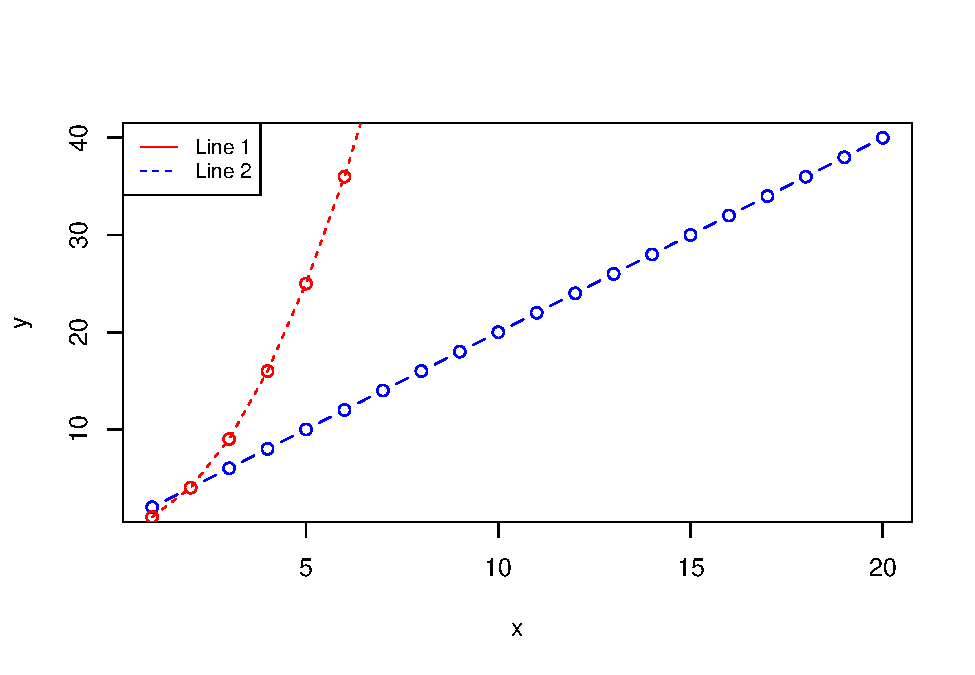
\includegraphics[width=0.7\linewidth]{EnvStat_files/figure-latex/line-1} 

}

\caption{Line plot}\label{fig:line}
\end{figure}

\section{Pie Chart}\label{pie-chart}

Pie chart digunakan untuk membuat visualisasi proporsi pada sebuah data.
Pie chart pada \texttt{R} dibuat menggunakan fungsi \texttt{pie()}.
Berikut adalah sintaks untuk membuat pie chart dan output yang
dihasilkan pada Figure \ref{fig:pie}:

\begin{Shaded}
\begin{Highlighting}[]
\KeywordTok{par}\NormalTok{(}\DataTypeTok{mar =} \KeywordTok{c}\NormalTok{(}\DecValTok{0}\NormalTok{, }\DecValTok{1}\NormalTok{, }\DecValTok{0}\NormalTok{, }\DecValTok{1}\NormalTok{))}
\KeywordTok{pie}\NormalTok{(}
  \KeywordTok{c}\NormalTok{(}\DecValTok{280}\NormalTok{, }\DecValTok{60}\NormalTok{, }\DecValTok{20}\NormalTok{),}
  \KeywordTok{c}\NormalTok{(}\StringTok{'Sky'}\NormalTok{, }\StringTok{'Sunny side of pyramid'}\NormalTok{, }\StringTok{'Shady side of pyramid'}\NormalTok{),}
  \DataTypeTok{col =} \KeywordTok{c}\NormalTok{(}\StringTok{'#0292D8'}\NormalTok{, }\StringTok{'#F7EA39'}\NormalTok{, }\StringTok{'#C4B632'}\NormalTok{),}
  \DataTypeTok{init.angle =} \OperatorTok{-}\DecValTok{50}\NormalTok{, }\DataTypeTok{border =} \OtherTok{NA}
\NormalTok{)}
\end{Highlighting}
\end{Shaded}

\begin{figure}

{\centering 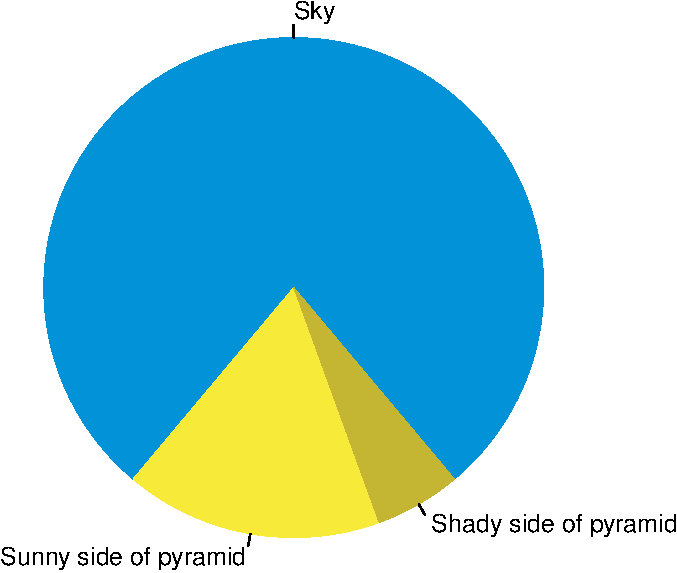
\includegraphics[width=0.7\linewidth]{EnvStat_files/figure-latex/pie-1} 

}

\caption{Pie chart}\label{fig:pie}
\end{figure}

\section{Histogram dan Density Plot}\label{histogram-dan-density-plot}

Fungsi \texttt{hist()} dapat digunakan untuk membuat histogram pada
\texttt{R}. Secara sederhana fungsi tersebut didefinisikan sebagai
berikut:

\begin{Shaded}
\begin{Highlighting}[]
\KeywordTok{hist}\NormalTok{(x, }\DataTypeTok{breaks=}\StringTok{"Sturges"}\NormalTok{)}
\end{Highlighting}
\end{Shaded}

\begin{quote}
\textbf{Note: }

\begin{itemize}
\tightlist
\item
  \textbf{x}: vektor numerik
\item
  \textbf{breaks}: \emph{breakpoints} antar sel histogram.
\end{itemize}
\end{quote}

Pada dataset \texttt{trees} akan dibuat histogram variabel
\texttt{Height}. Untuk melakukannya jalankan sintaks berikut:

\begin{Shaded}
\begin{Highlighting}[]
\KeywordTok{hist}\NormalTok{(trees}\OperatorTok{$}\NormalTok{Height)}
\end{Highlighting}
\end{Shaded}

Output yang dihasilkan disajikan pada Figure \ref{fig:hist}:

\begin{figure}

{\centering 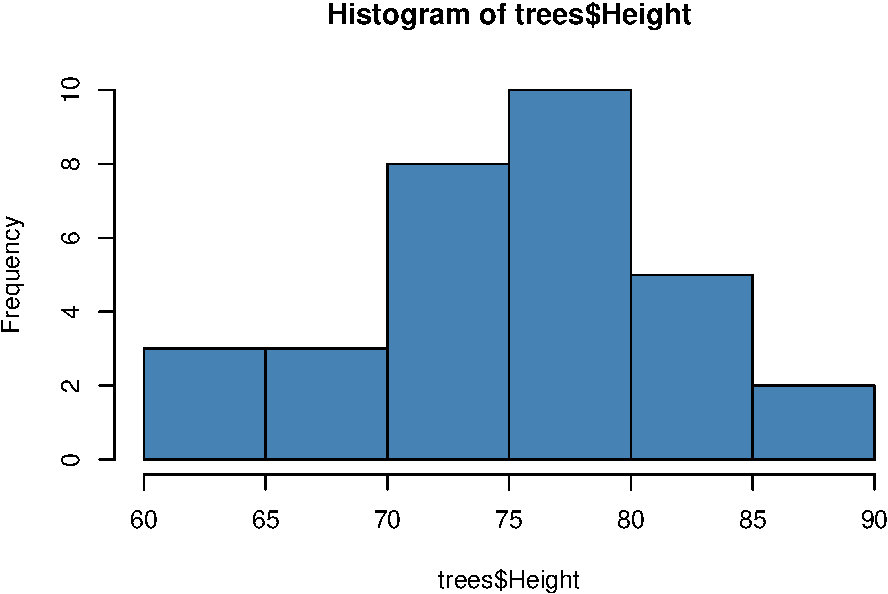
\includegraphics[width=0.7\linewidth]{EnvStat_files/figure-latex/hist-1} 

}

\caption{Histogram}\label{fig:hist}
\end{figure}

Density plot pada \texttt{R} dapat dibuat menggunakan fungsi
\texttt{density()}. Berbeda dengan fungsi \texttt{hist()}, fungsi ini
tidak langsung menghasilkan grafik densitas. Fungsi \texttt{density()}
hanya menghitung kernel densitas pada data. Densitas yang telah dihitung
selanjutnya diplotkan menggunakan fungsi \texttt{plot()}. Berikut adalah
sintaks dan output yang dihasilkan pada Figure \ref{fig:dens}:

\begin{Shaded}
\begin{Highlighting}[]
\CommentTok{# menghitung kernel density}
\NormalTok{dens <-}\StringTok{ }\KeywordTok{density}\NormalTok{(trees}\OperatorTok{$}\NormalTok{Height)}

\CommentTok{# plot densitas dengan outline merah}
\KeywordTok{plot}\NormalTok{(dens,}\DataTypeTok{col=}\StringTok{"red"}\NormalTok{)}
\end{Highlighting}
\end{Shaded}

\begin{figure}

{\centering 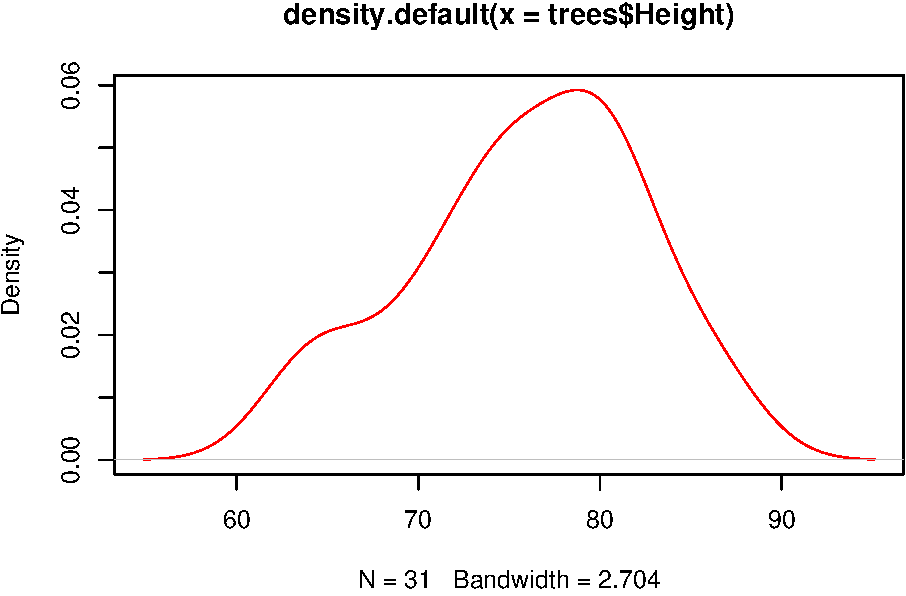
\includegraphics[width=0.7\linewidth]{EnvStat_files/figure-latex/dens-1} 

}

\caption{Density plot}\label{fig:dens}
\end{figure}

Kita juga dapat menambahkan grafik densitas pada histogram sehingga
mempermudah pembacaan pada histogram. Untuk melakukannya kita perlu
mengubah kernel histigram dari frekuensi menjadi density dengan
menambahkan argumen \texttt{freq=FALSE} pada fungsi \texttt{hist()}.
Selanjutnya tambahkan fungsi \texttt{polygon()} untuk memplotkan grafik
densitas. Berikut adalah sintak dan output yang dihasilkan pada Figure
\ref{fig:denshist}:

\begin{Shaded}
\begin{Highlighting}[]
\CommentTok{# menghitung kernel density}
\NormalTok{dens <-}\StringTok{ }\KeywordTok{density}\NormalTok{(trees}\OperatorTok{$}\NormalTok{Height)}

\CommentTok{# histogram}
\KeywordTok{hist}\NormalTok{(trees}\OperatorTok{$}\NormalTok{Height, }\DataTypeTok{freq=}\OtherTok{FALSE}\NormalTok{, }\DataTypeTok{col=}\StringTok{"steelblue"}\NormalTok{)}

\CommentTok{# tambahkan density plot}
\KeywordTok{polygon}\NormalTok{(dens, }\DataTypeTok{border=}\StringTok{"red"}\NormalTok{)}
\end{Highlighting}
\end{Shaded}

\begin{figure}

{\centering 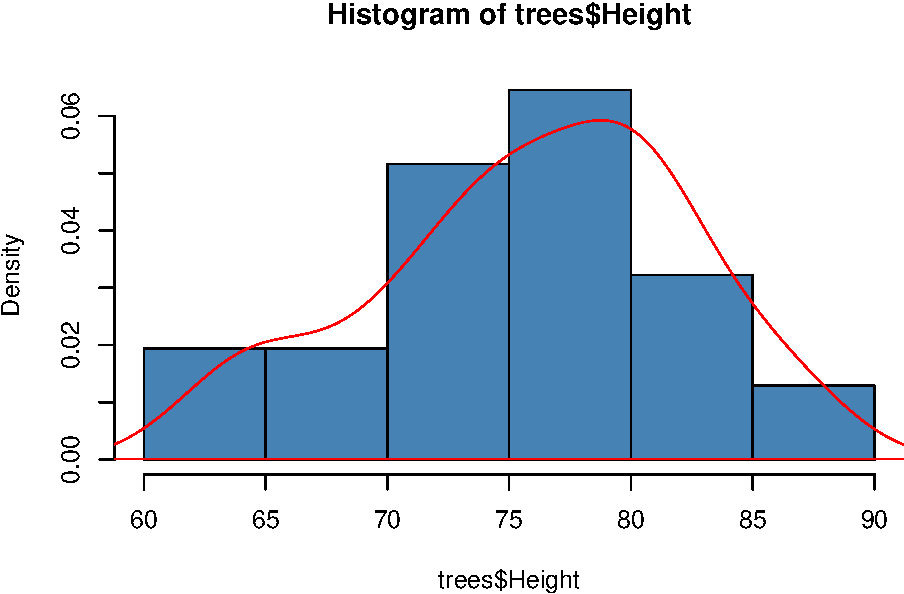
\includegraphics[width=0.7\linewidth]{EnvStat_files/figure-latex/denshist-1} 

}

\caption{Density plot dan histogram}\label{fig:denshist}
\end{figure}

\section{QQ Plot}\label{qq-plot}

QQ plot digunakan untuk mengecek distribusi suatu data apakah
berdistribusi normal atau tidak. Pada \texttt{R} QQ plot dibuat
menggunakan 2 fungsi yaitu: \texttt{qqnorm()} dan \texttt{qqline()}.
Fungsi \texttt{qqnorm()} digunakan untuk memproduksi normal QQ plot
suatu variabel. Sedangkan fungsi \texttt{qqline()} digunakan untuk
membuat garis referensi distiribusi normal. Suatu distribusi dikatan
normal jika titik observasi yang dihasilkan mengikuti garis referensi
tersebut.

Berikut adalah cara membuat QQ plot menggunakan variabel \texttt{Volume}
pada dataset \texttt{trees}. Output yang dihasilkan disajikan pada
Figure \ref{fig:qq}.

\begin{Shaded}
\begin{Highlighting}[]
\KeywordTok{qqnorm}\NormalTok{(trees}\OperatorTok{$}\NormalTok{Volume)}
\KeywordTok{qqline}\NormalTok{(trees}\OperatorTok{$}\NormalTok{Volume, }\DataTypeTok{col=}\StringTok{"red"}\NormalTok{)}
\end{Highlighting}
\end{Shaded}

\begin{figure}

{\centering 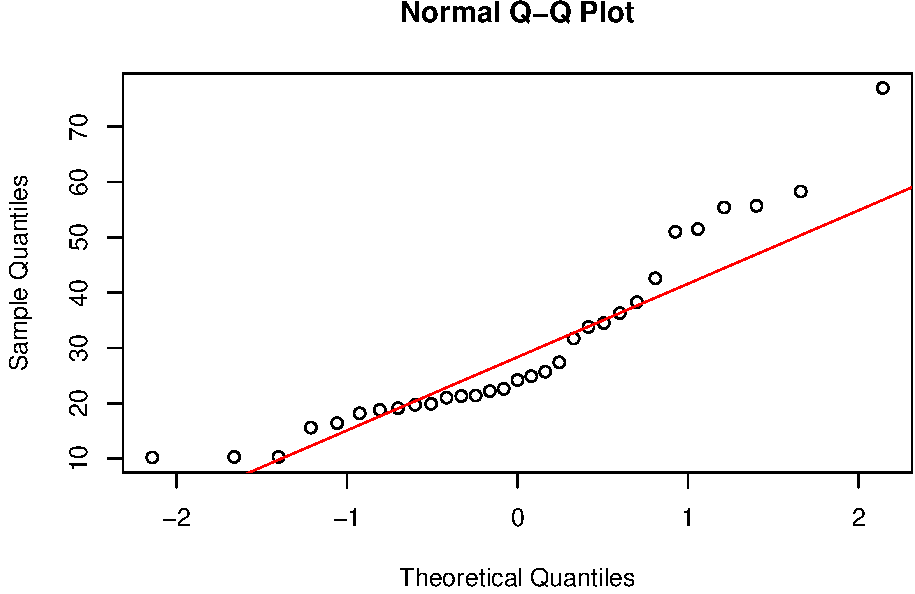
\includegraphics[width=0.7\linewidth]{EnvStat_files/figure-latex/qq-1} 

}

\caption{QQ plot}\label{fig:qq}
\end{figure}

\section{Dot Chart}\label{dot-chart}

Fungsi \texttt{dotchart()} pada \texttt{R} digunakan untuk membuat dot
chart. Format yang digunakan adalah sebagai berikut:

\begin{Shaded}
\begin{Highlighting}[]
\KeywordTok{dotchart}\NormalTok{(x, }\DataTypeTok{labels =} \OtherTok{NULL}\NormalTok{, }\DataTypeTok{groups =} \OtherTok{NULL}\NormalTok{, }
         \DataTypeTok{gcolor =} \KeywordTok{par}\NormalTok{(}\StringTok{"fg"}\NormalTok{), }\DataTypeTok{color =} \KeywordTok{par}\NormalTok{(}\StringTok{"fg"}\NormalTok{))}
\end{Highlighting}
\end{Shaded}

\begin{quote}
\textbf{Note: }

\begin{itemize}
\tightlist
\item
  \textbf{x}: vektor atau matriks numerik.
\item
  \textbf{labels}: vektor label untuk tiap titik.
\item
  \textbf{groups}: grouping variabel yang mengindikasikan bagaimana
  \textbf{x} dikelompokkan.
\item
  \textbf{gcolor}: warna yang digunakan pada label grup dan nilai
  observasi.
\item
  \textbf{color}: warna yang digunakan untuk titik dan label.
\end{itemize}
\end{quote}

Pada contoh berikut disajikan cara membuat dot chart pada dataset
\texttt{mtcars} untuk melihat mobil yang paling hemat bahan bakar
berdasarkan variabel \texttt{mpg} dan jumlah silinder (\texttt{cyl}).
Berikut sintaks yang digunakan dan output yang dihasilkan pada Figure
\ref{fig:dot}:

\begin{Shaded}
\begin{Highlighting}[]
\CommentTok{# mengurutkan dataset mtcars berdasarkan variabel mpg}
\NormalTok{mtcars <-}\StringTok{ }\NormalTok{mtcars[}\KeywordTok{order}\NormalTok{(mtcars}\OperatorTok{$}\NormalTok{mpg), ]}

\CommentTok{# mengubah variabel cyl menjadi factor}
\NormalTok{grps <-}\StringTok{ }\KeywordTok{as.factor}\NormalTok{(mtcars}\OperatorTok{$}\NormalTok{cyl)}

\CommentTok{# membuat vektor warna berdasarkan jumlah grup}
\NormalTok{my_cols <-}\StringTok{ }\KeywordTok{c}\NormalTok{(}\StringTok{"#999999"}\NormalTok{, }\StringTok{"#E69F00"}\NormalTok{, }\StringTok{"#56B4E9"}\NormalTok{)}

\CommentTok{# plot}
\KeywordTok{dotchart}\NormalTok{(mtcars}\OperatorTok{$}\NormalTok{mpg, }\DataTypeTok{labels =} \KeywordTok{row.names}\NormalTok{(mtcars),}
         \DataTypeTok{groups =}\NormalTok{ grps, }\DataTypeTok{gcolor =}\NormalTok{ my_cols,}
         \DataTypeTok{color =}\NormalTok{ my_cols[grps],}
         \DataTypeTok{cex =} \FloatTok{0.6}\NormalTok{,  }\DataTypeTok{pch =} \DecValTok{19}\NormalTok{, }\DataTypeTok{xlab =} \StringTok{"mpg"}\NormalTok{)}
\end{Highlighting}
\end{Shaded}

\begin{figure}

{\centering 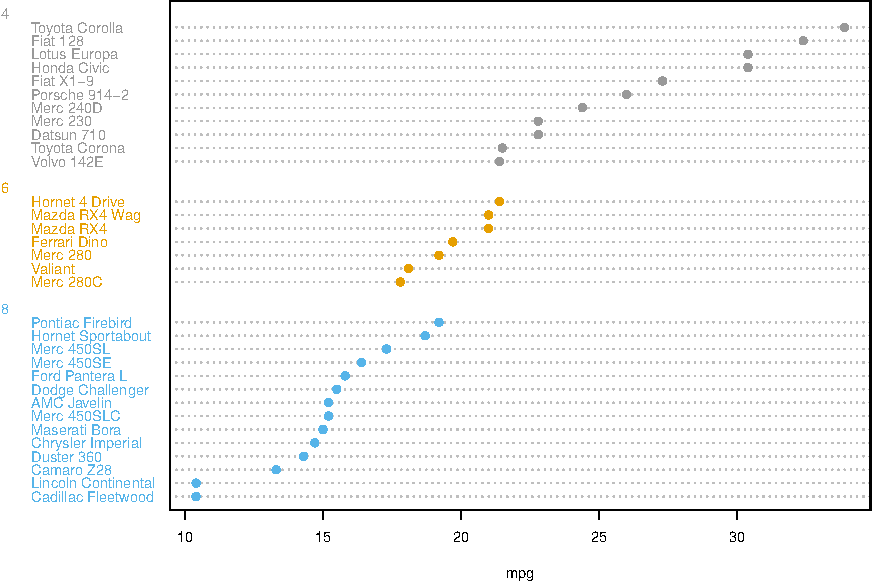
\includegraphics[width=0.7\linewidth]{EnvStat_files/figure-latex/dot-1} 

}

\caption{Dot chart}\label{fig:dot}
\end{figure}

\section{Kustomisasi Parameter
Grafik}\label{kustomisasi-parameter-grafik}

Pada bagian ini penulis akan menjelaskan cara untuk kustomisasi
parameter grafik seperti:

\begin{enumerate}
\def\labelenumi{\alph{enumi}.}
\tightlist
\item
  menambahkan judul, legend, teks, axis, dan garis.
\item
  mengubah skala axis, simbol plot, jenis garis, dan warna.
\end{enumerate}

\subsection{Menambahkan Judul}\label{menambahkan-judul}

Pada grafik di \texttt{R}, kita dapat menambahkan judul dengan dua cara,
yaitu: pada plot melalui parameter dan melalui fungsi plot(). Kedua cara
tersebut tidak berbeda satu sama lain pada parameter input.

Untuk menambahkan judul pada plot secara langsung, kita dapat
menggunakan argumen tambahan sebagai berikut:

\begin{enumerate}
\def\labelenumi{\alph{enumi}.}
\tightlist
\item
  \textbf{main}: teks untuk judul.
\item
  \textbf{xlab}: teks untuk keterangan axis X.
\item
  \textbf{ylab}: teks untuk keterangan axis y.
\item
  \textbf{sub}: teks untuk sub-judul.
\end{enumerate}

Berikut contoh sintaks penerapan masing-masing argumen tersebut beserta
dengan output yang dihasilkan pada Figure \ref{fig:title}:

\begin{Shaded}
\begin{Highlighting}[]
\CommentTok{# menambahkan judul}
\KeywordTok{barplot}\NormalTok{(}\KeywordTok{c}\NormalTok{(}\DecValTok{2}\NormalTok{,}\DecValTok{5}\NormalTok{), }\DataTypeTok{main=}\StringTok{"Main title"}\NormalTok{,}
        \DataTypeTok{xlab=}\StringTok{"X axis title"}\NormalTok{,}
        \DataTypeTok{ylab=}\StringTok{"Y axis title"}\NormalTok{,}
        \DataTypeTok{sub=}\StringTok{"Sub-title"}\NormalTok{)}
\end{Highlighting}
\end{Shaded}

\begin{figure}

{\centering 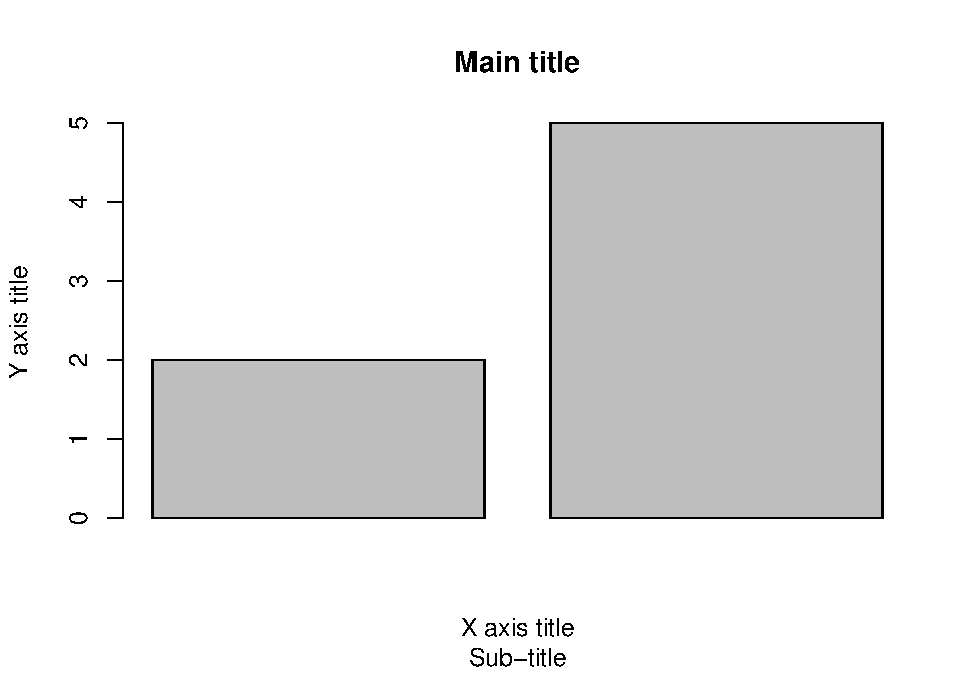
\includegraphics[width=0.7\linewidth]{EnvStat_files/figure-latex/title-1} 

}

\caption{Menambahkan Judul}\label{fig:title}
\end{figure}

kita juga dapat melakukan kustomisasi pada warna, \emph{font style}, dan
ukuran font judul. Untuk melakukan kustomisasi pada warna pada judul,
kita dapat menambahkan argumen sebagai berikut:

\begin{enumerate}
\def\labelenumi{\alph{enumi}.}
\tightlist
\item
  \textbf{col.main}: warna untuk judul.
\item
  \textbf{col.lab}: warna untuk keterangan axis.
\item
  \textbf{col.sub}: warna untuk sub-judul
\end{enumerate}

Untuk kustomisasi font judul, kita dapat menambahkan argumen berikut:

\begin{enumerate}
\def\labelenumi{\alph{enumi}.}
\tightlist
\item
  \textbf{font.main}: \emph{font style} untuk judul.
\item
  \textbf{font.lab}: \emph{font style} untuk keterangan axis.
\item
  \textbf{font.sub}: \emph{font style} untuk sub-judul.
\end{enumerate}

\begin{quote}
\textbf{Note: }

Nilai yang dapat dimasukkan antara lain:

\begin{itemize}
\tightlist
\item
  \textbf{1}: untuk teks normal.
\item
  \textbf{2}: untuk teks cetak tebal.
\item
  \textbf{3}: untuk teks cetak miring.
\item
  \textbf{4}: untuk teks cetak tebal dan miring.
\item
  \textbf{5}: untuk font simbol.
\end{itemize}
\end{quote}

Sedangkan untuk ukuran font, kita dapat menambahkan variabel berikut:

\begin{enumerate}
\def\labelenumi{\alph{enumi}.}
\tightlist
\item
  \textbf{cex.main}: ukuran teks judul.
\item
  \textbf{cex.lab}: ukuran teks keterangan axis.
\item
  \textbf{cex.sub}: ukuran teks sub-judul.
\end{enumerate}

Berikut sintaks penerapan seluruh argumen tersebut beserta output yang
dihasilkan pada Figure \ref{fig:title2}:

\begin{Shaded}
\begin{Highlighting}[]
\CommentTok{# menambahkan judul}
\KeywordTok{barplot}\NormalTok{(}\KeywordTok{c}\NormalTok{(}\DecValTok{2}\NormalTok{,}\DecValTok{5}\NormalTok{), }
        \CommentTok{# menambahkan judul}
        \DataTypeTok{main=}\StringTok{"Main title"}\NormalTok{,}
        \DataTypeTok{xlab=}\StringTok{"X axis title"}\NormalTok{,}
        \DataTypeTok{ylab=}\StringTok{"Y axis title"}\NormalTok{,}
        \DataTypeTok{sub=}\StringTok{"Sub-title"}\NormalTok{,}
        \CommentTok{# kustomisasi warna font}
        \DataTypeTok{col.main=}\StringTok{"red"}\NormalTok{, }
        \DataTypeTok{col.lab=}\StringTok{"blue"}\NormalTok{, }
        \DataTypeTok{col.sub=}\StringTok{"black"}\NormalTok{,}
        \CommentTok{# kustomisasi font style}
        \DataTypeTok{font.main=}\DecValTok{4}\NormalTok{, }
        \DataTypeTok{font.lab=}\DecValTok{4}\NormalTok{, }
        \DataTypeTok{font.sub=}\DecValTok{4}\NormalTok{,}
        \CommentTok{# kustomisasi ukuran font}
        \DataTypeTok{cex.main=}\DecValTok{2}\NormalTok{, }
        \DataTypeTok{cex.lab=}\FloatTok{1.7}\NormalTok{, }
        \DataTypeTok{cex.sub=}\FloatTok{1.2}\NormalTok{)}
\end{Highlighting}
\end{Shaded}

\begin{figure}

{\centering 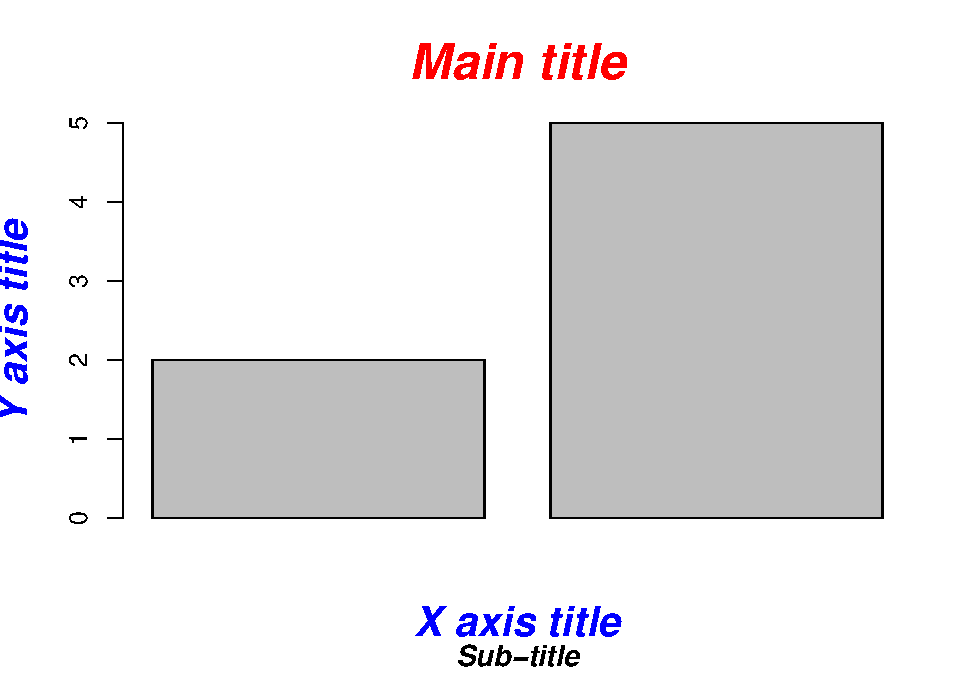
\includegraphics[width=0.7\linewidth]{EnvStat_files/figure-latex/title2-1} 

}

\caption{Menambahkan Judul (2)}\label{fig:title2}
\end{figure}

Kita telah belajar bagaimana menambahkan judul langsung pada fungsi
plot. Selain cara tersebut, telah penulis jelaskan bahwa kita dapat
menambahkan judul melalui fungsi \texttt{title()}. argumen yang
dimasukkan pada dasarnya tidak berbeda dengan ketika kita menambahkan
judul secara langsung pada plot. Berikut adalah contoh sintaks dan
output yang dihasilkan pada Figure \ref{fig:title3}:

\begin{Shaded}
\begin{Highlighting}[]
\CommentTok{# menambahkan judul}
\KeywordTok{barplot}\NormalTok{(}\KeywordTok{c}\NormalTok{(}\DecValTok{2}\NormalTok{,}\DecValTok{5}\NormalTok{,}\DecValTok{8}\NormalTok{))}

\CommentTok{# menambahkan judul}
\KeywordTok{title}\NormalTok{(}\DataTypeTok{main=}\StringTok{"Main title"}\NormalTok{,}
      \DataTypeTok{xlab=}\StringTok{"X axis title"}\NormalTok{,}
      \DataTypeTok{ylab=}\StringTok{"Y axis title"}\NormalTok{,}
      \DataTypeTok{sub=}\StringTok{"Sub-title"}\NormalTok{,}
      \CommentTok{# kustomisasi warna font}
      \DataTypeTok{col.main=}\StringTok{"red"}\NormalTok{, }
      \DataTypeTok{col.lab=}\StringTok{"blue"}\NormalTok{, }
      \DataTypeTok{col.sub=}\StringTok{"black"}\NormalTok{,}
      \CommentTok{# kustomisasi font style}
      \DataTypeTok{font.main=}\DecValTok{4}\NormalTok{, }
      \DataTypeTok{font.lab=}\DecValTok{4}\NormalTok{, }
      \DataTypeTok{font.sub=}\DecValTok{4}\NormalTok{,}
      \CommentTok{# kustomisasi ukuran font}
      \DataTypeTok{cex.main=}\DecValTok{2}\NormalTok{, }
      \DataTypeTok{cex.lab=}\FloatTok{1.7}\NormalTok{, }
      \DataTypeTok{cex.sub=}\FloatTok{1.2}\NormalTok{)}
\end{Highlighting}
\end{Shaded}

\begin{figure}

{\centering 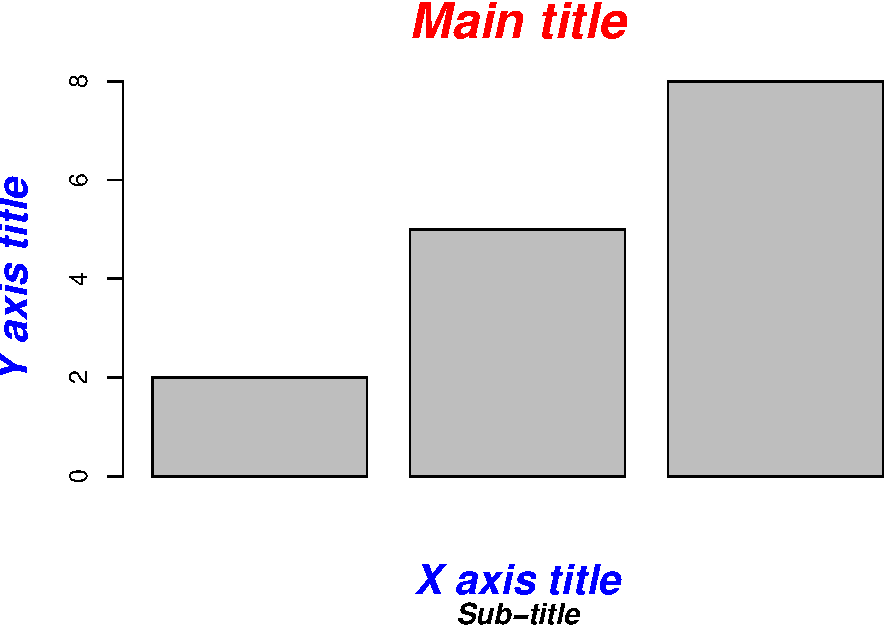
\includegraphics[width=0.7\linewidth]{EnvStat_files/figure-latex/title3-1} 

}

\caption{Menambahkan Judul (3)}\label{fig:title3}
\end{figure}

\subsection{Menambahkan Legend}\label{menambahkan-legend}

Fungsi \texttt{legend()} pada \texttt{R} dapat digunakan untuk
menambahkan legend pada grafik. Format sederhananya adalah sebagai
berikut:

\begin{Shaded}
\begin{Highlighting}[]
\KeywordTok{legend}\NormalTok{(x, }\DataTypeTok{y=}\OtherTok{NULL}\NormalTok{, legend, fill, col, bg)}
\end{Highlighting}
\end{Shaded}

\begin{quote}
\textbf{Note: }

\begin{itemize}
\tightlist
\item
  \textbf{x} dan \textbf{y}: koordinat yang digunakan untuk posisi
  legend.
\item
  \textbf{legend}: teks pada legend
\item
  \textbf{fill}: warna yang digunakan untuk mengisi box disamping teks
  legend.
\item
  \textbf{col}: warna garis dan titik disamping teks legend.
\item
  \textbf{bg}: warna latar belakang legend box.
\end{itemize}
\end{quote}

Berikut adalah contoh sintaks dan ouput penerapan argumen disajikan pada
Figure \ref{fig:legend}:

\begin{Shaded}
\begin{Highlighting}[]
\CommentTok{# membuat vektor numerik}
\NormalTok{x <-}\StringTok{ }\KeywordTok{c}\NormalTok{(}\DecValTok{1}\OperatorTok{:}\DecValTok{10}\NormalTok{)}
\NormalTok{y <-}\StringTok{ }\NormalTok{x}\OperatorTok{^}\DecValTok{2}
\NormalTok{z <-}\StringTok{ }\NormalTok{x}\OperatorTok{*}\DecValTok{2}

\CommentTok{# membuat line plot}
\KeywordTok{plot}\NormalTok{(x,y, }\DataTypeTok{type=}\StringTok{"o"}\NormalTok{, }\DataTypeTok{col=}\StringTok{"red"}\NormalTok{, }\DataTypeTok{lty=}\DecValTok{1}\NormalTok{)}

\CommentTok{# menambahkan line plot}
\KeywordTok{lines}\NormalTok{(x,z, }\DataTypeTok{type=}\StringTok{"o"}\NormalTok{, }\DataTypeTok{col=}\StringTok{"blue"}\NormalTok{, }\DataTypeTok{lty=}\DecValTok{2}\NormalTok{)}

\CommentTok{# menambahkan legend}
\KeywordTok{legend}\NormalTok{(}\DecValTok{1}\NormalTok{, }\DecValTok{95}\NormalTok{, }\DataTypeTok{legend=}\KeywordTok{c}\NormalTok{(}\StringTok{"Line 1"}\NormalTok{, }\StringTok{"Line 2"}\NormalTok{),}
       \DataTypeTok{col=}\KeywordTok{c}\NormalTok{(}\StringTok{"red"}\NormalTok{, }\StringTok{"blue"}\NormalTok{), }\DataTypeTok{lty=}\DecValTok{1}\OperatorTok{:}\DecValTok{2}\NormalTok{, }\DataTypeTok{cex=}\FloatTok{0.8}\NormalTok{)}
\end{Highlighting}
\end{Shaded}

\begin{figure}

{\centering 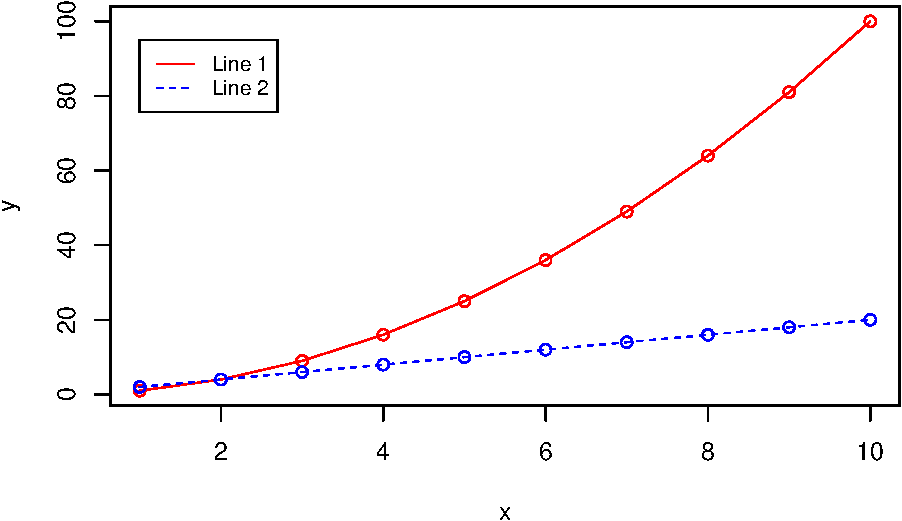
\includegraphics[width=0.7\linewidth]{EnvStat_files/figure-latex/legend-1} 

}

\caption{Menambahkan legend}\label{fig:legend}
\end{figure}

Kita dapat menambahkan judul, merubah font, dan merubah warna backgroud
pada legend. Argumen yang ditambahkan pada legend adalah sebagai
berikut:

\begin{enumerate}
\def\labelenumi{\alph{enumi}.}
\tightlist
\item
  \textbf{title}: Judul legend
\item
  \textbf{text.font}: integer yang menunjukkan \emph{font style} pada
  teks legend. Nilai yang dapat dimasukkan adalah sebagai berikut:

  \begin{itemize}
  \tightlist
  \item
    \textbf{1}: normal
  \item
    \textbf{2}: cetak tebal
  \item
    \textbf{3}: cetak miring
  \item
    \textbf{4}: cetak tebal dan miring.
  \end{itemize}
\item
  \textbf{bg}: warna background legend box.
\end{enumerate}

Berikut adalah penerapan sintaks dan output yang dihasilkan pada Figure
\ref{fig:legend2}:

\begin{Shaded}
\begin{Highlighting}[]
\CommentTok{# membuat line plot}
\KeywordTok{plot}\NormalTok{(x,y, }\DataTypeTok{type=}\StringTok{"o"}\NormalTok{, }\DataTypeTok{col=}\StringTok{"red"}\NormalTok{, }\DataTypeTok{lty=}\DecValTok{1}\NormalTok{)}

\CommentTok{# menambahkan line plot}
\KeywordTok{lines}\NormalTok{(x,z, }\DataTypeTok{type=}\StringTok{"o"}\NormalTok{, }\DataTypeTok{col=}\StringTok{"blue"}\NormalTok{, }\DataTypeTok{lty=}\DecValTok{2}\NormalTok{)}

\CommentTok{# menambahkan legend}
\KeywordTok{legend}\NormalTok{(}\DecValTok{1}\NormalTok{, }\DecValTok{95}\NormalTok{, }\DataTypeTok{legend=}\KeywordTok{c}\NormalTok{(}\StringTok{"Line 1"}\NormalTok{, }\StringTok{"Line 2"}\NormalTok{),}
       \DataTypeTok{col=}\KeywordTok{c}\NormalTok{(}\StringTok{"red"}\NormalTok{, }\StringTok{"blue"}\NormalTok{), }\DataTypeTok{lty=}\DecValTok{1}\OperatorTok{:}\DecValTok{2}\NormalTok{, }\DataTypeTok{cex=}\FloatTok{0.8}\NormalTok{,}
       \DataTypeTok{title=}\StringTok{"Line types"}\NormalTok{, }\DataTypeTok{text.font=}\DecValTok{4}\NormalTok{, }\DataTypeTok{bg=}\StringTok{'lightblue'}\NormalTok{)}
\end{Highlighting}
\end{Shaded}

\begin{figure}

{\centering 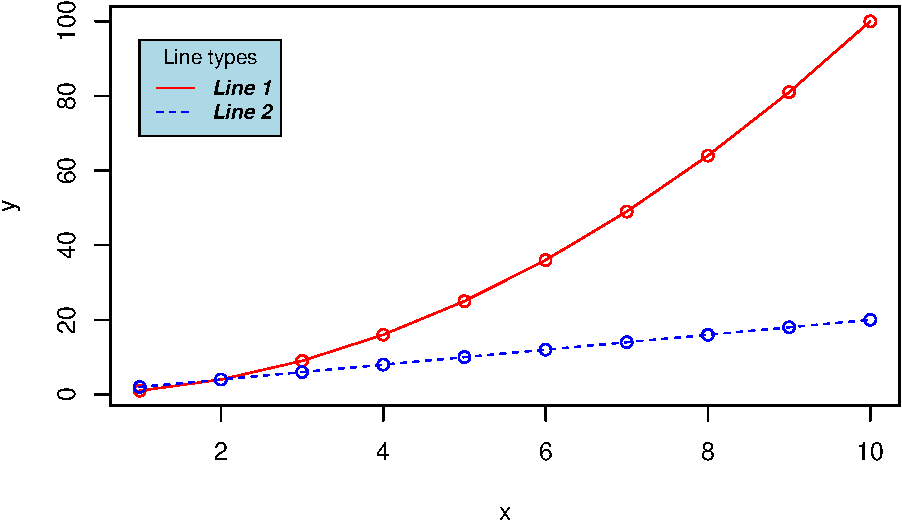
\includegraphics[width=0.7\linewidth]{EnvStat_files/figure-latex/legend2-1} 

}

\caption{Menambahkan legend (2)}\label{fig:legend2}
\end{figure}

Kita dapat melakukan kustomisasi pada border dari legend melalui argumen
\texttt{box.lty=}(jenis garis), \texttt{box.lwd=}(ukuran garis), dan
\texttt{box.col=}(warna box). Berikut adalah penerapan argumen tersebut
beserta output yang dihasilkan pada Figure \ref{fig:legend3}:

\begin{Shaded}
\begin{Highlighting}[]
\CommentTok{# membuat line plot}
\KeywordTok{plot}\NormalTok{(x,y, }\DataTypeTok{type=}\StringTok{"o"}\NormalTok{, }\DataTypeTok{col=}\StringTok{"red"}\NormalTok{, }\DataTypeTok{lty=}\DecValTok{1}\NormalTok{)}

\CommentTok{# menambahkan line plot}
\KeywordTok{lines}\NormalTok{(x,z, }\DataTypeTok{type=}\StringTok{"o"}\NormalTok{, }\DataTypeTok{col=}\StringTok{"blue"}\NormalTok{, }\DataTypeTok{lty=}\DecValTok{2}\NormalTok{)}

\CommentTok{# menambahkan legend}
\KeywordTok{legend}\NormalTok{(}\DecValTok{1}\NormalTok{, }\DecValTok{95}\NormalTok{, }\DataTypeTok{legend=}\KeywordTok{c}\NormalTok{(}\StringTok{"Line 1"}\NormalTok{, }\StringTok{"Line 2"}\NormalTok{),}
       \DataTypeTok{col=}\KeywordTok{c}\NormalTok{(}\StringTok{"red"}\NormalTok{, }\StringTok{"blue"}\NormalTok{), }\DataTypeTok{lty=}\DecValTok{1}\OperatorTok{:}\DecValTok{2}\NormalTok{, }\DataTypeTok{cex=}\FloatTok{0.8}\NormalTok{,}
       \DataTypeTok{title=}\StringTok{"Line types"}\NormalTok{, }\DataTypeTok{text.font=}\DecValTok{4}\NormalTok{, }\DataTypeTok{bg=}\StringTok{'white'}\NormalTok{,}
       \DataTypeTok{box.lty=}\DecValTok{2}\NormalTok{, }\DataTypeTok{box.lwd=}\DecValTok{2}\NormalTok{, }\DataTypeTok{box.col=}\StringTok{"steelblue"}\NormalTok{)}
\end{Highlighting}
\end{Shaded}

\begin{figure}

{\centering 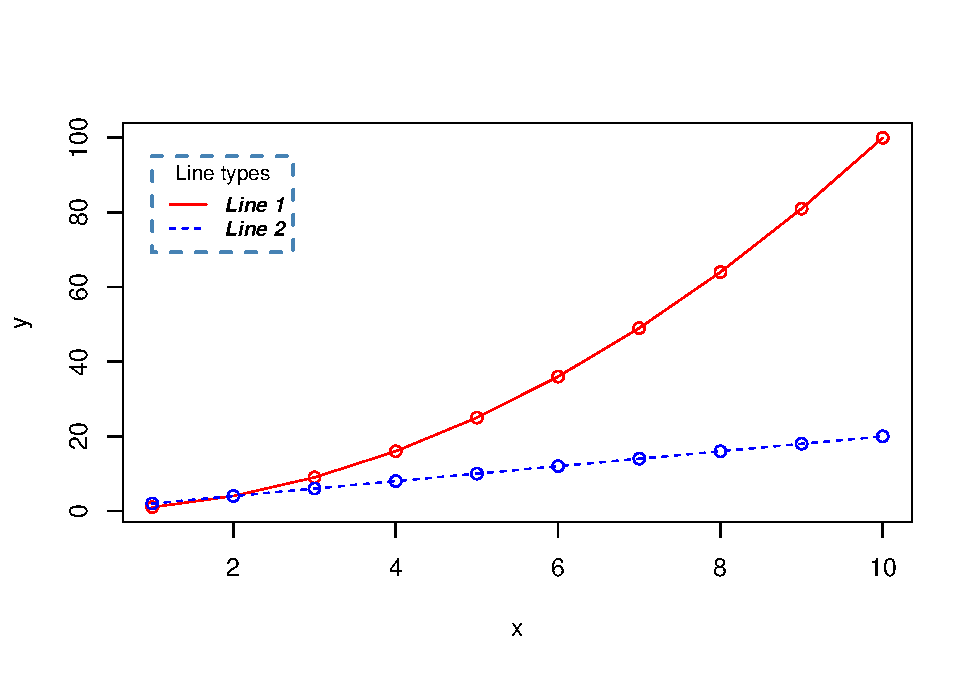
\includegraphics[width=0.7\linewidth]{EnvStat_files/figure-latex/legend3-1} 

}

\caption{Menambahkan legend (3)}\label{fig:legend3}
\end{figure}

Selain menggunakan koordinat, kita juga dapat melakukan kustomisasi
posisi legend menggunakan \emph{keyword} seperti:
bottomright``,''bottom``,''bottomleft``,''left``,''topleft``,''top``,''topright``,''right"
and ``center''. Sejumlah kustomisasi legend berdasarkan \emph{keyword}
disajikan pada Figure \ref{fig:legend4}:

\begin{Shaded}
\begin{Highlighting}[]
\CommentTok{# plot}
\KeywordTok{plot}\NormalTok{(x,y, }\DataTypeTok{type =} \StringTok{"n"}\NormalTok{)}

\CommentTok{# posisi kiri atas, inset =0.05}
\KeywordTok{legend}\NormalTok{(}\StringTok{"topleft"}\NormalTok{,}
  \DataTypeTok{legend =} \StringTok{"(x,y)"}\NormalTok{,}
  \DataTypeTok{title =} \StringTok{"topleft, inset = .05"}\NormalTok{,}
  \DataTypeTok{inset =} \FloatTok{0.05}\NormalTok{)}
\CommentTok{# posisi atas}
\KeywordTok{legend}\NormalTok{(}\StringTok{"top"}\NormalTok{,}
       \DataTypeTok{legend =} \StringTok{"(x,y)"}\NormalTok{,}
       \DataTypeTok{title =} \StringTok{"top"}\NormalTok{)}
\CommentTok{# posisi kanan atas inset = .02}
\KeywordTok{legend}\NormalTok{(}\StringTok{"topright"}\NormalTok{,}
       \DataTypeTok{legend =} \StringTok{"(x,y)"}\NormalTok{,}
       \DataTypeTok{title =} \StringTok{"topright, inset = .02"}\NormalTok{,}
       \DataTypeTok{inset =} \FloatTok{0.02}\NormalTok{)}
\CommentTok{# posisi kiri}
\KeywordTok{legend}\NormalTok{(}\StringTok{"left"}\NormalTok{,}
       \DataTypeTok{legend =} \StringTok{"(x,y)"}\NormalTok{,}
       \DataTypeTok{title =} \StringTok{"left"}\NormalTok{)}
\CommentTok{# posisi tengah}
\KeywordTok{legend}\NormalTok{(}\StringTok{"center"}\NormalTok{,}
       \DataTypeTok{legend =} \StringTok{"(x,y)"}\NormalTok{,}
       \DataTypeTok{title =} \StringTok{"center"}\NormalTok{)}
\CommentTok{# posisi kanan}
\KeywordTok{legend}\NormalTok{(}\StringTok{"right"}\NormalTok{,}
       \DataTypeTok{legend =} \StringTok{"(x,y)"}\NormalTok{,}
       \DataTypeTok{title =} \StringTok{"right"}\NormalTok{)}
\CommentTok{# posisi kiri bawah}
\KeywordTok{legend}\NormalTok{(}\StringTok{"bottomleft"}\NormalTok{,}
       \DataTypeTok{legend =} \StringTok{"(x,y)"}\NormalTok{,}
       \DataTypeTok{title =} \StringTok{"bottomleft"}\NormalTok{)}
\CommentTok{# posisi bawah}
\KeywordTok{legend}\NormalTok{(}\StringTok{"bottom"}\NormalTok{,}
       \DataTypeTok{legend =} \StringTok{"(x,y)"}\NormalTok{,}
       \DataTypeTok{title =} \StringTok{"bottom"}\NormalTok{)}
\CommentTok{# posisi kanan bawah}
\KeywordTok{legend}\NormalTok{(}\StringTok{"bottomright"}\NormalTok{,}
       \DataTypeTok{legend =} \StringTok{"(x,y)"}\NormalTok{,}
       \DataTypeTok{title =} \StringTok{"bottomright"}\NormalTok{)}
\end{Highlighting}
\end{Shaded}

\begin{figure}

{\centering 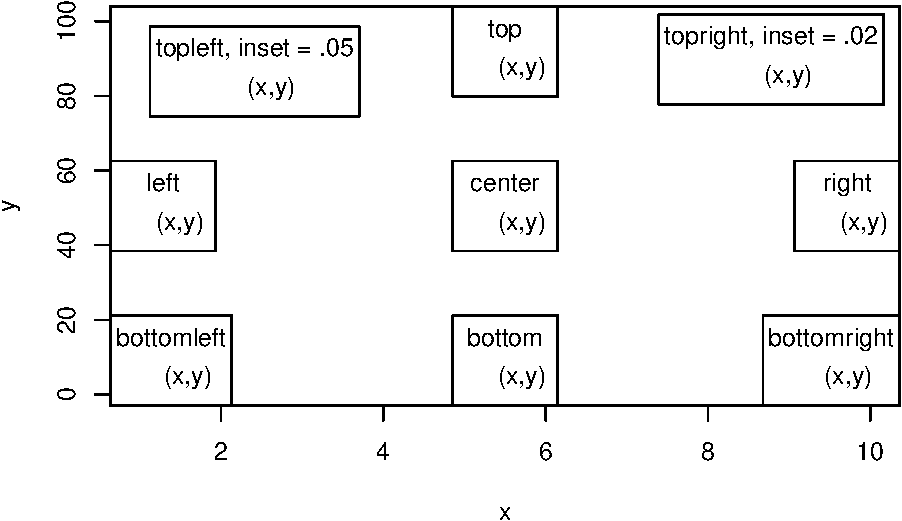
\includegraphics[width=0.7\linewidth]{EnvStat_files/figure-latex/legend4-1} 

}

\caption{Kustomisasi posisi legend}\label{fig:legend4}
\end{figure}

\subsection{Menambahkan Teks Pada
Grafik}\label{menambahkan-teks-pada-grafik}

Teks pada grafik dapat kita tambahkan baik sebagai keterangan yang
menunjukkan label suatu observasi, keterangan tambahan disekitar bingkai
grafik, maupun sebuah persamaan yang ada pada bidang grafik. Untuk
menambahkannya kita dapat menggunakan dua buah fungsi yaitu:
\texttt{text()} dan \texttt{mtext()}.

FUngsi \texttt{text()} berguna untuk menambahkan teks di dalam bidang
grafik seperti label titik observasi dan persamaan di dalam bidang
grafik. Format yang digunakan adalah sebagai berikut:

\begin{Shaded}
\begin{Highlighting}[]
\KeywordTok{text}\NormalTok{(x, y, labels)}
\end{Highlighting}
\end{Shaded}

\begin{quote}
\textbf{Note: }

\begin{itemize}
\tightlist
\item
  \textbf{x} dan \textbf{y}: vektor numerik yang menunjukkan koordinat
  posisi teks.
\item
  \textbf{labels}: vektor karakter yang menunjukkan teks yang hendak
  ditulis.
\end{itemize}
\end{quote}

Berikut adalah contoh sintaks untuk memberi label pada sejumlah data
yang memiliki kriteria yang kita inginkan dan output yang dihasilkan
pada Figure \ref{fig:text}:

\begin{Shaded}
\begin{Highlighting}[]
\CommentTok{# tandai observasi yang memiliki nilai}
\CommentTok{# mpg < 15 dan wt > 5}
\NormalTok{d <-}\StringTok{ }\NormalTok{mtcars[mtcars}\OperatorTok{$}\NormalTok{wt }\OperatorTok{>=}\StringTok{ }\DecValTok{5} \OperatorTok{&}\StringTok{ }\NormalTok{mtcars}\OperatorTok{$}\NormalTok{mpg }\OperatorTok{<=}\StringTok{ }\DecValTok{15}\NormalTok{, ]}


\CommentTok{# plot}
\KeywordTok{plot}\NormalTok{(mtcars}\OperatorTok{$}\NormalTok{wt, mtcars}\OperatorTok{$}\NormalTok{mpg, }\DataTypeTok{main=}\StringTok{"Milage vs. Car Weight"}\NormalTok{,}
      \DataTypeTok{xlab=}\StringTok{"Weight"}\NormalTok{, }\DataTypeTok{ylab=}\StringTok{"Miles/(US) gallon"}\NormalTok{)}

\CommentTok{# menambahkan text}
\KeywordTok{text}\NormalTok{(d}\OperatorTok{$}\NormalTok{wt, d}\OperatorTok{$}\NormalTok{mpg,  }\KeywordTok{row.names}\NormalTok{(d),}
     \DataTypeTok{cex=}\FloatTok{0.65}\NormalTok{, }\DataTypeTok{pos=}\DecValTok{3}\NormalTok{,}\DataTypeTok{col=}\StringTok{"red"}\NormalTok{)}
\end{Highlighting}
\end{Shaded}

\begin{figure}

{\centering 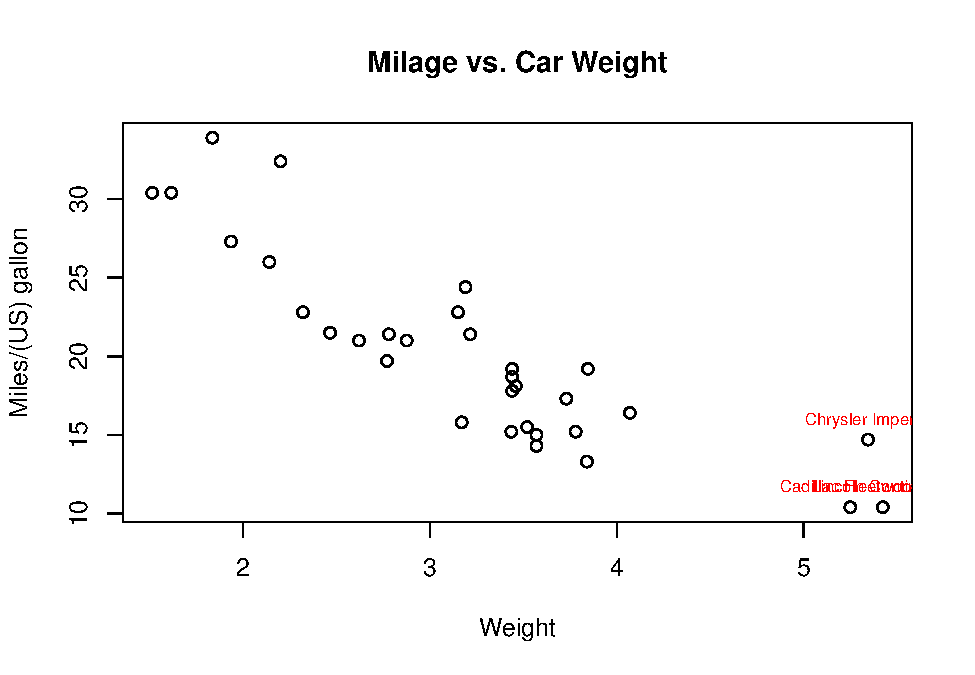
\includegraphics[width=0.7\linewidth]{EnvStat_files/figure-latex/text-1} 

}

\caption{Menambahkan teks}\label{fig:text}
\end{figure}

Sedangkan sintaks berikut adalah contoh bagaimana menambahkan persamaan
kedalam bidang grafik dan output yang dihasilkan pada Figure
\ref{fig:text2}:

\begin{Shaded}
\begin{Highlighting}[]
\KeywordTok{plot}\NormalTok{(}\DecValTok{1}\OperatorTok{:}\DecValTok{10}\NormalTok{, }\DecValTok{1}\OperatorTok{:}\DecValTok{10}\NormalTok{, }
     \DataTypeTok{main=}\StringTok{"text(...) examples}\CharTok{\textbackslash{}n}\StringTok{~~~~~~~~~~~"}\NormalTok{)}
\KeywordTok{text}\NormalTok{(}\DecValTok{4}\NormalTok{, }\DecValTok{9}\NormalTok{, }\KeywordTok{expression}\NormalTok{(}\KeywordTok{hat}\NormalTok{(beta) }\OperatorTok{==}\StringTok{ }\NormalTok{(X}\OperatorTok{^}\NormalTok{t }\OperatorTok{*}\StringTok{ }\NormalTok{X)}\OperatorTok{^}\NormalTok{\{}\OperatorTok{-}\DecValTok{1}\NormalTok{\} }\OperatorTok{*}\StringTok{ }\NormalTok{X}\OperatorTok{^}\NormalTok{t }\OperatorTok{*}\StringTok{ }\NormalTok{y))}
\KeywordTok{text}\NormalTok{(}\DecValTok{7}\NormalTok{, }\DecValTok{4}\NormalTok{, }\KeywordTok{expression}\NormalTok{(}\KeywordTok{bar}\NormalTok{(x) }\OperatorTok{==}\StringTok{ }\KeywordTok{sum}\NormalTok{(}\KeywordTok{frac}\NormalTok{(x[i], n), i}\OperatorTok{==}\DecValTok{1}\NormalTok{, n)))}
\end{Highlighting}
\end{Shaded}

\begin{figure}

{\centering 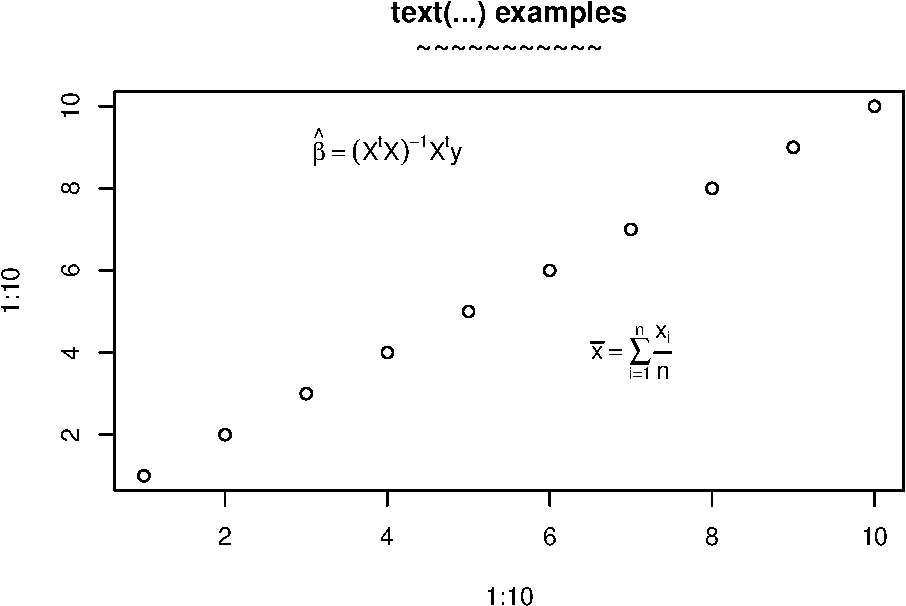
\includegraphics[width=0.7\linewidth]{EnvStat_files/figure-latex/text2-1} 

}

\caption{Menambahkan teks (2)}\label{fig:text2}
\end{figure}

Fungsi \texttt{mtext()} berguna untuk menambahkan teks pada frame
sekitar bidang grafik. Format yang digunakan adalah sebagai berikut:

\begin{Shaded}
\begin{Highlighting}[]
\KeywordTok{mtext}\NormalTok{(text, }\DataTypeTok{side=}\DecValTok{3}\NormalTok{)}
\end{Highlighting}
\end{Shaded}

\begin{quote}
\textbf{Note: }

\begin{itemize}
\tightlist
\item
  \textbf{text}: teks yang akan ditulis.
\item
  \textbf{side}: integer yang menunjukkan lokasi teks yang akan ditulis.
  Nilai yang dapat dimasukkan antara lain:
\item
  \textbf{1}: bawah
\item
  \textbf{2}: kiri
\item
  \textbf{3}: atas
\item
  \textbf{4}: kanan.
\end{itemize}
\end{quote}

Berikut adalah contoh penerapan dan output yang dihasilkan pada Figure
\ref{fig:text3}:

\begin{Shaded}
\begin{Highlighting}[]
\KeywordTok{plot}\NormalTok{(}\DecValTok{1}\OperatorTok{:}\DecValTok{10}\NormalTok{, }\DecValTok{1}\OperatorTok{:}\DecValTok{10}\NormalTok{, }
     \DataTypeTok{main=}\StringTok{"mtext(...) examples}\CharTok{\textbackslash{}n}\StringTok{~~~~~~~~~~~"}\NormalTok{)}
\KeywordTok{mtext}\NormalTok{(}\StringTok{"Magic function"}\NormalTok{, }\DataTypeTok{side=}\DecValTok{3}\NormalTok{)}
\end{Highlighting}
\end{Shaded}

\begin{figure}

{\centering 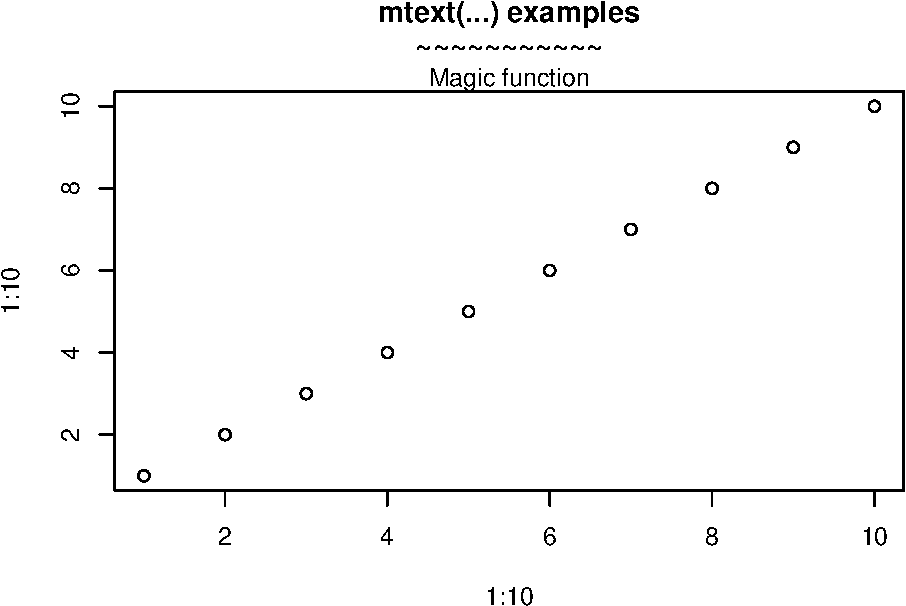
\includegraphics[width=0.7\linewidth]{EnvStat_files/figure-latex/text3-1} 

}

\caption{Menambahkan teks (3)}\label{fig:text3}
\end{figure}

\subsection{Menambahkan Garis Pada
Plot}\label{menambahkan-garis-pada-plot}

Fungsi \texttt{abline()} dapat digunakan untuk menamabahkan garis pada
plot. Garis yang ditambahkan dapat berupa garis vertikal, horizontal,
maupun garis regresi. Format yang digunakan adalah sebagi berikut:

\begin{Shaded}
\begin{Highlighting}[]
\KeywordTok{abline}\NormalTok{(}\DataTypeTok{v=}\NormalTok{y)}
\end{Highlighting}
\end{Shaded}

Berikut adalah contoh sintaks bagaimana menambahkan garis pada sebuah
plot dan output yang dihasilkan disajikan pada Figure \ref{fig:abline}:

\begin{Shaded}
\begin{Highlighting}[]
\CommentTok{# membuat plot}
\KeywordTok{plot}\NormalTok{(mtcars}\OperatorTok{$}\NormalTok{wt, mtcars}\OperatorTok{$}\NormalTok{mpg, }\DataTypeTok{main=}\StringTok{"Milage vs. Car Weight"}\NormalTok{,}
      \DataTypeTok{xlab=}\StringTok{"Weight"}\NormalTok{, }\DataTypeTok{ylab=}\StringTok{"Miles/(US) gallon"}\NormalTok{)}

\CommentTok{# menambahkan garis vertikal di titik rata-rata weight}
\KeywordTok{abline}\NormalTok{(}\DataTypeTok{v=}\KeywordTok{mean}\NormalTok{(mtcars}\OperatorTok{$}\NormalTok{wt), }\DataTypeTok{col=}\StringTok{"red"}\NormalTok{, }\DataTypeTok{lwd=}\DecValTok{3}\NormalTok{, }\DataTypeTok{lty=}\DecValTok{2}\NormalTok{)}

\CommentTok{# menambahkan garis horizontal di titik rata-rata  mpg}
\KeywordTok{abline}\NormalTok{(}\DataTypeTok{h=}\KeywordTok{mean}\NormalTok{(mtcars}\OperatorTok{$}\NormalTok{mpg), }\DataTypeTok{col=}\StringTok{"blue"}\NormalTok{, }\DataTypeTok{lwd=}\DecValTok{3}\NormalTok{, }\DataTypeTok{lty=}\DecValTok{3}\NormalTok{)}

\CommentTok{# menambahkan garis regresi}
\KeywordTok{abline}\NormalTok{(}\KeywordTok{lm}\NormalTok{(mpg}\OperatorTok{~}\NormalTok{wt, }\DataTypeTok{data=}\NormalTok{mtcars), }\DataTypeTok{lwd=}\DecValTok{4}\NormalTok{, }\DataTypeTok{lty=}\DecValTok{4}\NormalTok{)}
\end{Highlighting}
\end{Shaded}

\begin{figure}

{\centering 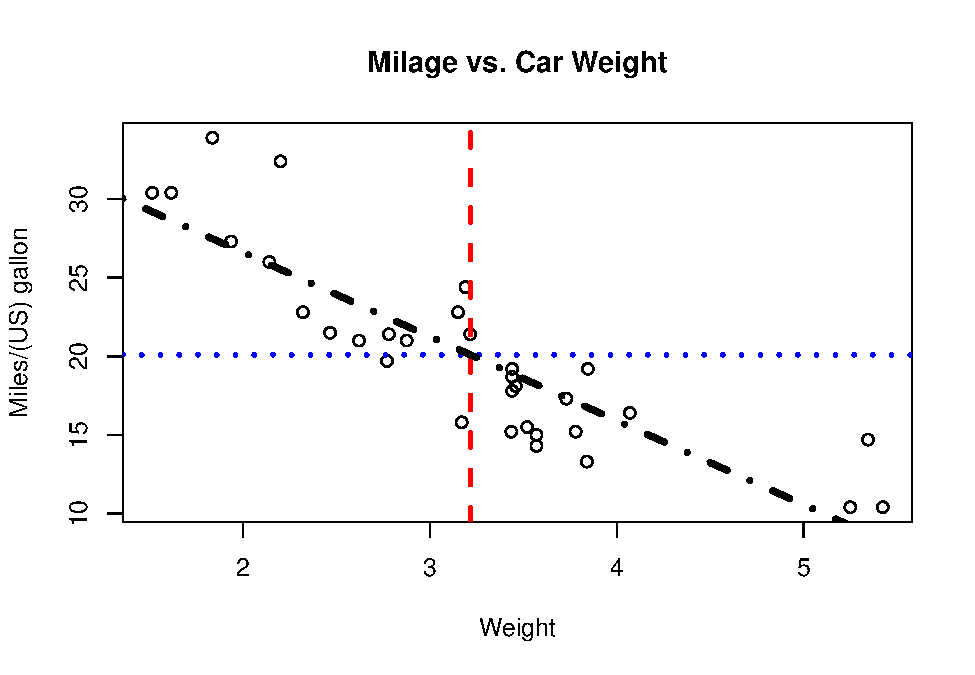
\includegraphics[width=0.7\linewidth]{EnvStat_files/figure-latex/abline-1} 

}

\caption{Menambahkan garis}\label{fig:abline}
\end{figure}

\subsection{Merubah Simbol plot dan Jenis
Garis}\label{merubah-simbol-plot-dan-jenis-garis}

Simbol plot (jenis titik) dapat diubah dengan menambahkan argumen
\texttt{pch=} pada plot. Nilai yang dimasukkan pada argumen tersebut
adalah integer dengan kemungkinan nilai sebagai berikut:

\begin{itemize}
\tightlist
\item
  pch = 0,square
\item
  pch = 1,circle (default)
\item
  pch = 2,triangle point up
\item
  pch = 3,plus
\item
  pch = 4,cross
\item
  pch = 5,diamond
\item
  pch = 6,triangle point down
\item
  pch = 7,square cross
\item
  pch = 8,star
\item
  pch = 9,diamond plus
\item
  pch = 10,circle plus
\item
  pch = 11,triangles up and down
\item
  pch = 12,square plus
\item
  pch = 13,circle cross
\item
  pch = 14,square and triangle down
\item
  pch = 15, filled square
\item
  pch = 16, filled circle
\item
  pch = 17, filled triangle point-up
\item
  pch = 18, filled diamond
\item
  pch = 19, solid circle
\item
  pch = 20,bullet (smaller circle)
\item
  pch = 21, filled circle blue
\item
  pch = 22, filled square blue
\item
  pch = 23, filled diamond blue
\item
  pch = 24, filled triangle point-up blue
\item
  pch = 25, filled triangle point down blue
\end{itemize}

Untuk lebih memahami bentuk simbol tersebut, penulis akan menyajikan
sintaks yang menampilkan seluruh simbol tersebut pada satu grafik.
Output yang dihasilkan disajikan pada Figure \ref{fig:symbol}:

\begin{Shaded}
\begin{Highlighting}[]
\NormalTok{generateRPointShapes<-}\ControlFlowTok{function}\NormalTok{()\{}
  \CommentTok{# menentukan parameter plot}
\NormalTok{  oldPar<-}\KeywordTok{par}\NormalTok{()}
  \KeywordTok{par}\NormalTok{(}\DataTypeTok{font=}\DecValTok{2}\NormalTok{, }\DataTypeTok{mar=}\KeywordTok{c}\NormalTok{(}\FloatTok{0.5}\NormalTok{,}\DecValTok{0}\NormalTok{,}\DecValTok{0}\NormalTok{,}\DecValTok{0}\NormalTok{))}
  \CommentTok{# produksi titik axis}
\NormalTok{  y=}\KeywordTok{rev}\NormalTok{(}\KeywordTok{c}\NormalTok{(}\KeywordTok{rep}\NormalTok{(}\DecValTok{1}\NormalTok{,}\DecValTok{6}\NormalTok{),}\KeywordTok{rep}\NormalTok{(}\DecValTok{2}\NormalTok{,}\DecValTok{5}\NormalTok{), }\KeywordTok{rep}\NormalTok{(}\DecValTok{3}\NormalTok{,}\DecValTok{5}\NormalTok{), }\KeywordTok{rep}\NormalTok{(}\DecValTok{4}\NormalTok{,}\DecValTok{5}\NormalTok{), }\KeywordTok{rep}\NormalTok{(}\DecValTok{5}\NormalTok{,}\DecValTok{5}\NormalTok{)))}
\NormalTok{  x=}\KeywordTok{c}\NormalTok{(}\KeywordTok{rep}\NormalTok{(}\DecValTok{1}\OperatorTok{:}\DecValTok{5}\NormalTok{,}\DecValTok{5}\NormalTok{),}\DecValTok{6}\NormalTok{)}
  \CommentTok{# plot seluruh titik dan label}
  \KeywordTok{plot}\NormalTok{(x, y, }\DataTypeTok{pch =} \DecValTok{0}\OperatorTok{:}\DecValTok{25}\NormalTok{, }\DataTypeTok{cex=}\FloatTok{1.5}\NormalTok{, }\DataTypeTok{ylim=}\KeywordTok{c}\NormalTok{(}\DecValTok{1}\NormalTok{,}\FloatTok{5.5}\NormalTok{), }\DataTypeTok{xlim=}\KeywordTok{c}\NormalTok{(}\DecValTok{1}\NormalTok{,}\FloatTok{6.5}\NormalTok{), }
       \DataTypeTok{axes=}\OtherTok{FALSE}\NormalTok{, }\DataTypeTok{xlab=}\StringTok{""}\NormalTok{, }\DataTypeTok{ylab=}\StringTok{""}\NormalTok{, }\DataTypeTok{bg=}\StringTok{"blue"}\NormalTok{)}
  \KeywordTok{text}\NormalTok{(x, y, }\DataTypeTok{labels=}\DecValTok{0}\OperatorTok{:}\DecValTok{25}\NormalTok{, }\DataTypeTok{pos=}\DecValTok{3}\NormalTok{)}
  \KeywordTok{par}\NormalTok{(}\DataTypeTok{mar=}\NormalTok{oldPar}\OperatorTok{$}\NormalTok{mar,}\DataTypeTok{font=}\NormalTok{oldPar}\OperatorTok{$}\NormalTok{font )}
\NormalTok{\}}

\CommentTok{# Print}
\KeywordTok{generateRPointShapes}\NormalTok{()}
\end{Highlighting}
\end{Shaded}

\begin{figure}

{\centering \includegraphics[width=0.7\linewidth]{EnvStat_files/figure-latex/symbol-1} 

}

\caption{Symbol plot}\label{fig:symbol}
\end{figure}

Pada \texttt{R} kita juga dapat mengatur jenis garis yang akan
ditampilkan pada plot dengan menambahkan argumen \texttt{lty=}
(\emph{line type}) pada fungsi plot. Nilai yang dapat dimasukkan adalah
nilai integer. Keterangan masing-masing nilai tersebut adalah sebagai
berikut:

\begin{itemize}
\tightlist
\item
  lty = 0, blank
\item
  lty = 1, solid (default)
\item
  lty = 2, dashed
\item
  lty = 3, dotted
\item
  lty = 4, dotdash
\item
  lty = 5, longdash
\item
  lty = 6, twodash
\end{itemize}

Untuk lebih memahaminya, pada sintaks berikut disajikan plot seluruh
jenis garis tersebut beserta output yang dihasilkannya pada Figure
\ref{fig:lty}:

\begin{Shaded}
\begin{Highlighting}[]
\NormalTok{generateRLineTypes<-}\ControlFlowTok{function}\NormalTok{()\{}
\NormalTok{  oldPar<-}\KeywordTok{par}\NormalTok{()}
  \KeywordTok{par}\NormalTok{(}\DataTypeTok{font=}\DecValTok{2}\NormalTok{, }\DataTypeTok{mar=}\KeywordTok{c}\NormalTok{(}\DecValTok{0}\NormalTok{,}\DecValTok{0}\NormalTok{,}\DecValTok{0}\NormalTok{,}\DecValTok{0}\NormalTok{))}
  \KeywordTok{plot}\NormalTok{(}\DecValTok{1}\NormalTok{, }\DataTypeTok{pch=}\StringTok{""}\NormalTok{, }\DataTypeTok{ylim=}\KeywordTok{c}\NormalTok{(}\DecValTok{0}\NormalTok{,}\DecValTok{6}\NormalTok{), }\DataTypeTok{xlim=}\KeywordTok{c}\NormalTok{(}\DecValTok{0}\NormalTok{,}\FloatTok{0.7}\NormalTok{), }\DataTypeTok{axes =} \OtherTok{FALSE}\NormalTok{ ,}\DataTypeTok{xlab=}\StringTok{""}\NormalTok{, }\DataTypeTok{ylab=}\StringTok{""}\NormalTok{)}
  \ControlFlowTok{for}\NormalTok{(i }\ControlFlowTok{in} \DecValTok{0}\OperatorTok{:}\DecValTok{6}\NormalTok{) }\KeywordTok{lines}\NormalTok{(}\KeywordTok{c}\NormalTok{(}\FloatTok{0.3}\NormalTok{,}\FloatTok{0.7}\NormalTok{), }\KeywordTok{c}\NormalTok{(i,i), }\DataTypeTok{lty=}\NormalTok{i, }\DataTypeTok{lwd=}\DecValTok{3}\NormalTok{)}
  \KeywordTok{text}\NormalTok{(}\KeywordTok{rep}\NormalTok{(}\FloatTok{0.1}\NormalTok{,}\DecValTok{6}\NormalTok{), }\DecValTok{0}\OperatorTok{:}\DecValTok{6}\NormalTok{, }
       \DataTypeTok{labels=}\KeywordTok{c}\NormalTok{(}\StringTok{"0.'blank'"}\NormalTok{, }\StringTok{"1.'solid'"}\NormalTok{, }\StringTok{"2.'dashed'"}\NormalTok{, }\StringTok{"3.'dotted'"}\NormalTok{, }
                \StringTok{"4.'dotdash'"}\NormalTok{, }\StringTok{"5.'longdash'"}\NormalTok{, }\StringTok{"6.'twodash'"}\NormalTok{))}
  \KeywordTok{par}\NormalTok{(}\DataTypeTok{mar=}\NormalTok{oldPar}\OperatorTok{$}\NormalTok{mar,}\DataTypeTok{font=}\NormalTok{oldPar}\OperatorTok{$}\NormalTok{font )}
\NormalTok{\}}
\KeywordTok{generateRLineTypes}\NormalTok{()}
\end{Highlighting}
\end{Shaded}

\begin{figure}

{\centering \includegraphics[width=0.7\linewidth]{EnvStat_files/figure-latex/lty-1} 

}

\caption{Line type}\label{fig:lty}
\end{figure}

\subsection{Mengatur Axis Plot}\label{mengatur-axis-plot}

Kita dapat melakukan pengaturan lebih jauh terhadap axis, seperti:
menambahkan axis tambahan pada atas dan bawah frame, mengubah rentang
nilai axis, serta kustomisasi \emph{tick mark} pada nilai axis. Hal ini
diperlukan karena fungsi grafik dasar \texttt{R} tidak dapat mengatur
axis secara otomatis saat plot baru ditambahkan pada plot pertama dan
rentang nilai plot baru lebih besar dibanding plot pertama, sehingga
sebagian nilai plot baru tidak ditampilkan pada hasil akhir.

Untuk menambahkan axis pada \texttt{R} kita dapat menambahkan fungsi
\texttt{axis()} setelah plot dilakukan. Format yang digunakan adalah
sebagai berikut:

\begin{Shaded}
\begin{Highlighting}[]
\KeywordTok{axis}\NormalTok{(side, }\DataTypeTok{at=}\OtherTok{NULL}\NormalTok{, }\DataTypeTok{labels=}\OtherTok{TRUE}\NormalTok{)}
\end{Highlighting}
\end{Shaded}

\begin{quote}
\textbf{Note: }

\begin{itemize}
\tightlist
\item
  \textbf{side}: nilai integer yang mengidikasikan posisi axix yang
  hendak ditambahkan. Nilai yang dapat dimasukkan adalah sebagai
  berikut:

  \begin{itemize}
  \tightlist
  \item
    \textbf{1}: bawah
  \item
    \textbf{2}: kiri
  \item
    \textbf{3}: atas
  \item
    \textbf{4}: kanan.
  \end{itemize}
\item
  \textbf{at}: titik dimana \emph{tick-mark} hendak digambarkan. Nilai
  yang dapat dimasukkan sama dengan \textbf{side}.
\item
  \textbf{labels}: Teks label \emph{tick-mark}. Dapat juga secara logis
  menentukan apakah anotasi harus dibuat pada \emph{tick mark}.
\end{itemize}
\end{quote}

Berikut contoh sintaks penerapan fungsi tersebut dan output yang
dihasilkan pada Figure \ref{fig:axis}:

\begin{Shaded}
\begin{Highlighting}[]
\CommentTok{# membuat vektor numerik}
\NormalTok{x <-}\StringTok{ }\KeywordTok{c}\NormalTok{(}\DecValTok{1}\OperatorTok{:}\DecValTok{4}\NormalTok{)}
\NormalTok{y <-}\StringTok{ }\NormalTok{x}\OperatorTok{^}\DecValTok{2}

\CommentTok{# plot}
\KeywordTok{plot}\NormalTok{(x, y, }\DataTypeTok{pch=}\DecValTok{18}\NormalTok{, }\DataTypeTok{col=}\StringTok{"red"}\NormalTok{, }\DataTypeTok{type=}\StringTok{"b"}\NormalTok{,}
     \DataTypeTok{frame=}\OtherTok{FALSE}\NormalTok{, }\DataTypeTok{xaxt=}\StringTok{"n"}\NormalTok{) }\CommentTok{# Remove x axis}

\CommentTok{# menambahkan axis}
\CommentTok{# bawah}
\KeywordTok{axis}\NormalTok{(}\DecValTok{1}\NormalTok{, }\DecValTok{1}\OperatorTok{:}\DecValTok{4}\NormalTok{, LETTERS[}\DecValTok{1}\OperatorTok{:}\DecValTok{4}\NormalTok{], }\DataTypeTok{col.axis=}\StringTok{"blue"}\NormalTok{)}
\CommentTok{# atas}
\KeywordTok{axis}\NormalTok{(}\DecValTok{3}\NormalTok{, }\DataTypeTok{col =} \StringTok{"darkgreen"}\NormalTok{, }\DataTypeTok{lty =} \DecValTok{2}\NormalTok{, }\DataTypeTok{lwd =} \FloatTok{0.5}\NormalTok{)}
\CommentTok{# kanan}
\KeywordTok{axis}\NormalTok{(}\DecValTok{4}\NormalTok{, }\DataTypeTok{col =} \StringTok{"violet"}\NormalTok{, }\DataTypeTok{col.axis =} \StringTok{"dark violet"}\NormalTok{, }\DataTypeTok{lwd =} \DecValTok{2}\NormalTok{)}
\end{Highlighting}
\end{Shaded}

\begin{figure}

{\centering \includegraphics[width=0.7\linewidth]{EnvStat_files/figure-latex/axis-1} 

}

\caption{Menambahkan axis}\label{fig:axis}
\end{figure}

Kita dapat mengubah rentang nilai pada axis menggunakan fungsi
\texttt{xlim()} dan \texttt{ylim()} yang menyatakan vektor nilai masimum
dan minimum rentang. Selain itu kita dapat juga melakukan tranformasi
baik pada sumbu x dan sumbu y. Berikut adalah argumen yang dapat
ditambahkan pada fungsi grafik:

\begin{itemize}
\tightlist
\item
  \textbf{xlim}: limit nilai sumbu x dengan format:
  \texttt{xlim(min,\ max)}.
\item
  \textbf{ylim}: limit nilai sumbu x dengan format:
  \texttt{ylim(min,\ max)}.
\end{itemize}

Untuk transformasi skala log, kita dapat menambahkan argumen berikut:

\begin{itemize}
\tightlist
\item
  \textbf{log=``x''}: transformasi log sumbu x.
\item
  \textbf{log=``y''}: transformasi log sumbu y.
\item
  \textbf{log=``xy''}: transformasi log sumbu x dan y.
\end{itemize}

Berikut adalah contoh sintaks penerapan argumen tersebut beserta output
yang dihasilkan pada Figure \ref{fig:axis2}:

\begin{Shaded}
\begin{Highlighting}[]
\CommentTok{# membagi jendela grafik menjadi 1 baris dan 3 kolom}
\KeywordTok{par}\NormalTok{(}\DataTypeTok{mfrow=}\KeywordTok{c}\NormalTok{(}\DecValTok{1}\NormalTok{,}\DecValTok{3}\NormalTok{))}

\CommentTok{# membuat vektor numerik}
\NormalTok{x<-}\KeywordTok{c}\NormalTok{(}\DecValTok{1}\OperatorTok{:}\DecValTok{10}\NormalTok{); y<-x}\OperatorTok{*}\NormalTok{x}

\CommentTok{# simple plot}
\KeywordTok{plot}\NormalTok{(x, y)}

\CommentTok{# plot dengan pengaturan rentang skala}
\KeywordTok{plot}\NormalTok{(x, y, }\DataTypeTok{xlim=}\KeywordTok{c}\NormalTok{(}\DecValTok{1}\NormalTok{,}\DecValTok{15}\NormalTok{), }\DataTypeTok{ylim=}\KeywordTok{c}\NormalTok{(}\DecValTok{1}\NormalTok{,}\DecValTok{150}\NormalTok{))}

\CommentTok{# plot dengan transformasi skala log}
\KeywordTok{plot}\NormalTok{(x, y, }\DataTypeTok{log=}\StringTok{"y"}\NormalTok{)}
\end{Highlighting}
\end{Shaded}

\begin{figure}

{\centering \includegraphics[width=0.8\linewidth]{EnvStat_files/figure-latex/axis2-1} 

}

\caption{Mengubah rentang dan skala axis}\label{fig:axis2}
\end{figure}

Kita dapat melakukan kustomisasi pada \emph{tick mark}. Kustomisasi yang
dapat dilakukan adalah merubah warna, \emph{font style}, ukuran font,
orientasi, serta menyembunyikan \emph{tick mark}.

Argumen yang ditambahkan adalah sebagai berikut:

\begin{itemize}
\item
  \textbf{col.axis}: warna \emph{tick mark}.
\item
  \textbf{font.axis}: integer yang menunjukkan \emph{font style}. Sama
  dengan pengaturan judul.
\item
  \textbf{cex.axis}: pengaturan ukuran \emph{tick mark}.
\item
  \textbf{las}: mengatur orientasi \emph{tick mark}. Nilai yang dapat
  dimasukkan adalah sebagai berikut:
\item
  \textbf{0}: paralel terhadap posisi axis (default)
\item
  \textbf{1}: selalu horizontal
\item
  \textbf{2}: selalu perpendikular dengan posisi axis
\item
  \textbf{3}: selalu vertikal
\item
  \textbf{xaxt} dan \textbf{yaxt}: karakter untuk menunjukkan apakah
  axis akan ditampilkan atau tidak. nilai dapat berupa ``n''(sembunyika)
  dan ``s''(tampilkan).
\end{itemize}

Berikut adalah contoh penerapan argumen tersebut beserta output pada
Figure \ref{fig:axis3}:

\begin{Shaded}
\begin{Highlighting}[]
\CommentTok{# membuat vektor numerik}
\NormalTok{x<-}\KeywordTok{c}\NormalTok{(}\DecValTok{1}\OperatorTok{:}\DecValTok{10}\NormalTok{); y<-x}\OperatorTok{*}\NormalTok{x}

\CommentTok{# plot}
\KeywordTok{plot}\NormalTok{(x,y,}
     \CommentTok{# warna}
     \DataTypeTok{col.axis=}\StringTok{"red"}\NormalTok{,}
     \CommentTok{# font style}
     \DataTypeTok{font.axis=}\DecValTok{2}\NormalTok{,}
     \CommentTok{# ukuran}
     \DataTypeTok{cex=}\FloatTok{1.5}\NormalTok{,}
     \CommentTok{# orientasi}
     \DataTypeTok{las=}\DecValTok{3}\NormalTok{,}
     \CommentTok{# sembunyikan sumbu x}
     \DataTypeTok{xaxt=}\StringTok{"n"}\NormalTok{)}
\end{Highlighting}
\end{Shaded}

\begin{figure}

{\centering \includegraphics[width=0.7\linewidth]{EnvStat_files/figure-latex/axis3-1} 

}

\caption{Kustomisasi tick mark}\label{fig:axis3}
\end{figure}

\subsection{Mengatur Warna}\label{mengatur-warna}

Pada fungsi dasar \texttt{R}, warna dapat diatur dengan mengetikkan nama
warna maupun kode hexadesimal. Selain itu kita juga dapat menamambahkan
warna lain melalui library lain yang tidak dijelaskan pada chapter ini.

Untuk penggunaan warna hexadesima kita perlu mengetikkan ``\#'' yang
diukuti oleh 6 kode warna. Untuk memperlajari kode-kode dan warna yang
dihasilkan, silahkan pembaca mengunjungi situs
\url{http://www.visibone.com/}.

Pada sintaks berikut disajikan visualisasi nama-nama warna bawaan yang
ada pada \texttt{R}. Output yang dihasilkan disajikan pada Figure
\ref{fig:color}:

\begin{Shaded}
\begin{Highlighting}[]
\NormalTok{showCols <-}\StringTok{ }\ControlFlowTok{function}\NormalTok{(}\DataTypeTok{cl=}\KeywordTok{colors}\NormalTok{(), }\DataTypeTok{bg =} \StringTok{"grey"}\NormalTok{,}
                     \DataTypeTok{cex =} \FloatTok{0.75}\NormalTok{, }\DataTypeTok{rot =} \DecValTok{30}\NormalTok{) \{}
\NormalTok{    m <-}\StringTok{ }\KeywordTok{ceiling}\NormalTok{(}\KeywordTok{sqrt}\NormalTok{(n <-}\KeywordTok{length}\NormalTok{(cl)))}
    \KeywordTok{length}\NormalTok{(cl) <-}\StringTok{ }\NormalTok{m}\OperatorTok{*}\NormalTok{m; cm <-}\StringTok{ }\KeywordTok{matrix}\NormalTok{(cl, m)}
    \KeywordTok{require}\NormalTok{(}\StringTok{"grid"}\NormalTok{)}
    \KeywordTok{grid.newpage}\NormalTok{(); vp <-}\StringTok{ }\KeywordTok{viewport}\NormalTok{(}\DataTypeTok{w =}\NormalTok{ .}\DecValTok{92}\NormalTok{, }\DataTypeTok{h =}\NormalTok{ .}\DecValTok{92}\NormalTok{)}
    \KeywordTok{grid.rect}\NormalTok{(}\DataTypeTok{gp=}\KeywordTok{gpar}\NormalTok{(}\DataTypeTok{fill=}\NormalTok{bg))}
    \KeywordTok{grid.text}\NormalTok{(cm, }\DataTypeTok{x =} \KeywordTok{col}\NormalTok{(cm)}\OperatorTok{/}\NormalTok{m, }\DataTypeTok{y =} \KeywordTok{rev}\NormalTok{(}\KeywordTok{row}\NormalTok{(cm))}\OperatorTok{/}\NormalTok{m, }\DataTypeTok{rot =}\NormalTok{ rot,}
              \DataTypeTok{vp=}\NormalTok{vp, }\DataTypeTok{gp=}\KeywordTok{gpar}\NormalTok{(}\DataTypeTok{cex =}\NormalTok{ cex, }\DataTypeTok{col =}\NormalTok{ cm))}
\NormalTok{\}}

\CommentTok{# print 60 nama warna pertama}
\KeywordTok{showCols}\NormalTok{(}\DataTypeTok{bg=}\StringTok{"gray20"}\NormalTok{, }\DataTypeTok{cl=}\KeywordTok{colors}\NormalTok{()[}\DecValTok{1}\OperatorTok{:}\DecValTok{60}\NormalTok{], }\DataTypeTok{rot=}\DecValTok{30}\NormalTok{, }\DataTypeTok{cex=}\FloatTok{0.9}\NormalTok{)}
\end{Highlighting}
\end{Shaded}

\begin{figure}

{\centering \includegraphics[width=0.7\linewidth]{EnvStat_files/figure-latex/color-1} 

}

\caption{Nama warna}\label{fig:color}
\end{figure}

\section{Alternatif Library Dasar
Lain}\label{alternatif-library-dasar-lain}

Kita juga dapat melakukan visualisasi menggunakan library lain yang
memiliki tampilan mirip dengan fungsi visualisasi dasar \texttt{R}.
Bedanya adalah library-library ini memberikan fungsi tambahan sehingga
visualisasi yang dihasilkan menjadi lebih praktis.

\subsection{Scatterplot Menggunakan Library
car}\label{scatterplot-menggunakan-library-car}

Library \texttt{car} menyediakan alternatif lain visualisasi menggunakan
scatterplot. Berikut adalah contoh sintaks dan output yang dihasilkan
pada Figure \ref{fig:carscatter}:

\begin{Shaded}
\begin{Highlighting}[]
\CommentTok{# memasang paket}
\CommentTok{# install.packages("car")}

\CommentTok{# memuat paket}
\KeywordTok{library}\NormalTok{(car)}

\CommentTok{# plot}
\KeywordTok{scatterplot}\NormalTok{(Volume}\OperatorTok{~}\NormalTok{Height, }\DataTypeTok{data=}\NormalTok{trees)}
\end{Highlighting}
\end{Shaded}

\begin{figure}

{\centering \includegraphics[width=0.7\linewidth]{EnvStat_files/figure-latex/carscatter-1} 

}

\caption{Enhanced scatterplot}\label{fig:carscatter}
\end{figure}

Pada grafik tersebut terkandung beberapa elemen penting, yaitu:

\begin{itemize}
\tightlist
\item
  titik observasi
\item
  garis regresi (garis lurus)
\item
  non-parametric regression smooth (\emph{dashed line})
\item
  garis smoothed conditional (\emph{point dashed line})
\item
  box plot masing-masing variabel.
\end{itemize}

\subsection{Matriks Scatterplot Menggunakan Library
psych}\label{matriks-scatterplot-menggunakan-library-psych}

FUngsi \texttt{pairs.panels()} pada library \texttt{psych} dapat
digunakan untuk membuat matriks scatterplot. Grafik yang dihasilkan juga
lebih ringkas dan menampilkan fungsional lain pada bagian diagonal lain
berupa histogram dan density plot yang dapat menunjukkan distribusi dari
variabel yang ada. Selain itu pada fungsionalitas grafik juga dapat
ditingkatkan dengan penambahan nilai korelasi antar variabel yang secara
default ditambahkan pada panel atas. Berikut adalah contoh sintaks dan
output yang dihasilkan pada Figure \ref{fig:psychscatter}:

\begin{Shaded}
\begin{Highlighting}[]
\CommentTok{# memasang paket}
\CommentTok{# install.packages("psych")}

\CommentTok{# memuat paket}
\KeywordTok{library}\NormalTok{(psych)}

\CommentTok{# plot}
\KeywordTok{pairs.panels}\NormalTok{(trees, }
             \DataTypeTok{method =} \StringTok{"pearson"}\NormalTok{, }\CommentTok{# metode korelasi}
             \DataTypeTok{hist.col =} \StringTok{"grey"}\NormalTok{,}
             \DataTypeTok{density =} \OtherTok{TRUE}\NormalTok{,  }\CommentTok{# menampilkan plot densitas}
             \DataTypeTok{ellipses =} \OtherTok{FALSE}\NormalTok{, }\CommentTok{# menampilkancorrelation ellipses}
             \DataTypeTok{lm =} \OtherTok{TRUE} \CommentTok{# menampilkan garis regresi linier}
\NormalTok{             )}
\end{Highlighting}
\end{Shaded}

\begin{figure}

{\centering \includegraphics[width=0.7\linewidth]{EnvStat_files/figure-latex/psychscatter-1} 

}

\caption{Enhanced scatterplot matrices}\label{fig:psychscatter}
\end{figure}

\subsection{Box Plot Menggunakan Library
gplots}\label{box-plot-menggunakan-library-gplots}

Fungsi \texttt{boxplot2()} pada paket \texttt{gplots} memberikan
fungsionalitas lebih dibandingkan box plot yang dihasilkan dari fungsi
dasar \texttt{R}. Plot yang dihasilkan akan menampilkan jumlah observasi
pada tiap box. Berikut adalah contoh sintask penerapan dan output yang
dihasilkan pada Figure \ref{fig:gplotsboxplot2}:

\begin{Shaded}
\begin{Highlighting}[]
\CommentTok{# memasang paket}
\CommentTok{# install.packages("gplots")}

\CommentTok{# memuat paket}
\KeywordTok{library}\NormalTok{(gplots)}

\CommentTok{# plot}
\KeywordTok{boxplot2}\NormalTok{(len }\OperatorTok{~}\StringTok{ }\NormalTok{dose, }\DataTypeTok{data =}\NormalTok{ ToothGrowth)}
\end{Highlighting}
\end{Shaded}

\begin{figure}

{\centering \includegraphics[width=0.7\linewidth]{EnvStat_files/figure-latex/gplotsboxplot2-1} 

}

\caption{Enhanced box plot}\label{fig:gplotsboxplot2}
\end{figure}

\subsection{QQ Plot Menggunakan Library
car}\label{qq-plot-menggunakan-library-car}

Fungsi \texttt{qqPlot()} pada library \texttt{car} dapat pula digunakan
untuk membuat qq plot. Kelebihannya adalah qqplot yang dihasilkan akan
dilengkapi dengan garis referensi yang memudahkan dalam membaca apakah
data masih dalam rentang distribusi normal atau tidak. Selain itu, untuk
membuatnya juga hanya diperlukan satu perintah saja. Hal ini tentu
berbeda ketika kita menggunakan fungsi dasar \texttt{R}. Berikut adalah
contoh sintask penerapan dan output yang dihasilkan pada Figure
\ref{fig:carqqplot}:

\begin{Shaded}
\begin{Highlighting}[]
\CommentTok{# memasang paket}
\CommentTok{# install.packages("car")}

\CommentTok{# memuat paket}
\KeywordTok{library}\NormalTok{(car)}

\CommentTok{# plot}
\KeywordTok{qqPlot}\NormalTok{(trees}\OperatorTok{$}\NormalTok{Height)}
\end{Highlighting}
\end{Shaded}

\begin{figure}

{\centering \includegraphics[width=0.7\linewidth]{EnvStat_files/figure-latex/carqqplot-1} 

}

\caption{Enhanced qq plot}\label{fig:carqqplot}
\end{figure}

\begin{verbatim}
## [1]  3 20
\end{verbatim}

\subsection{Plot Group Means Menggunakan Library
gplots}\label{plot-group-means-menggunakan-library-gplots}

Plot ini akan sering kita gunakan saat melakukan analisis statistik
menggunakan anova baik anova satu arah maupun dua arah. Plot ini berguna
untuk melihat adanya interaksi antar faktor saat melakukan analisis
anova dua arah. Berikut adalah contoh sintask penerapan dan output yang
dihasilkan pada Figure \ref{fig:plotmeans}:

\begin{Shaded}
\begin{Highlighting}[]
\CommentTok{# memasang paket}
\CommentTok{# install.packages("gplots")}

\CommentTok{# memuat paket}
\KeywordTok{library}\NormalTok{(gplots)}

\CommentTok{# plot}
\KeywordTok{plotmeans}\NormalTok{(len }\OperatorTok{~}\StringTok{ }\NormalTok{dose, }\DataTypeTok{data =}\NormalTok{ ToothGrowth)}
\end{Highlighting}
\end{Shaded}

\begin{figure}

{\centering \includegraphics[width=0.7\linewidth]{EnvStat_files/figure-latex/plotmeans-1} 

}

\caption{Plot group means}\label{fig:plotmeans}
\end{figure}

\section{Referensi}\label{referensi-3}

\begin{enumerate}
\def\labelenumi{\arabic{enumi}.}
\tightlist
\item
  Maindonald, J.H. 2008. \textbf{Using R for Data Analysis and Graphics
  Introduction, Code and Commentary}. Centre for Mathematics and Its
  Applications Australian National University.
\item
  Scherber, C. 2007. \textbf{An introduction to statistical data
  analysis using R}. R\_Manual Goettingen.
\item
  Venables, W.N. Smith D.M. and R Core Team. 2018. \textbf{An
  Introduction to R}. R Manuals.
\item
  STHDA. \textbf{R Base Graphs}.
  \url{http://www.sthda.com/english/wiki/r-base-graphs}
\end{enumerate}

\chapter{Final Words}\label{final-words}

We have finished a nice book.

\bibliography{book.bib,packages.bib}


\end{document}
